
\documentclass[oneside]{book}

\usepackage{template_professor}

\begin{document}
\pagecolor{special!13 }

% Public domain font used here (http://www.1001freefonts.com/homemade_apple.font) should be install to use properly
% Notebook page definition

\def\Bg{\newpage
 \vspace*{-1.2cm}
 \thispagestyle{empty}
\hspace{-2cm} \begin{tikzpicture}[anchor=north, normal lines/.style={gray, very thin}, every node/.append style={black, align=center, opacity=1}]
    \foreach \y in {0.71,1.41,...,25.56}
      \draw[normal lines, lightgray] (0,\y) -- (8.1 in,\y);
    \draw[normal lines, attention] (2cm,0) -- (2cm,11in);
     \node (t) [ font=\LARGE, anchor=south] at ($(0,25.76)!1/2!(7.8 in,25.76)$) {\fontspec{Homemade Apple} Notas de Aula};
  \end{tikzpicture}%
\quad
\newpage
}

\pagenumbering{gobble}



\noindent {\color{special}{\Large \bf LIÇÃO 1 - Para o professor}}
\vspace{.5cm}

Esta lição tem por objetivo introduzir frações unitárias a partir de modelos visuais contínuos, tais como ``discos'', ``retângulos'', ``hexágonos'' e ``segmentos'', fazendo uso de expressões verbais como, por exemplo, ``metade de...'', ``um terço de...'', ``a terça parte de...'', ``um quarto de...'', para indicar essas frações.
A expressão ``fração unitária'' nomeia cada uma das partes da divisão de uma unidade em partes iguais.

As atividades visam à equipartição de uma unidade. Equipartição entendida como partição em partes iguais, sem que as partes tenham necessariamente a mesma forma. Assim, por exemplo, na equipartição de um retângulo está implícito que as partes têm a mesma área, e não necessariamente a mesma forma nem o mesmo perímetro. O objetivo é levar o aluno a reconhecer diferentes modos de dividir e recompor a unidade. No senso comum, as expressões repartir, partir e dividir são sinônimas e não pressupõem a equipartição. No entanto, é importante lembrar que, no caso da operação de divisão, espera-se que o resultado registre uma equipartição. No futuro, o estudante deverá entender um terço como o resultado da divisão de um por três. Este é o caso da operação, em que a palavra ``divisão'' abrevia ``divisão em partes iguais''.

Espera-se que, ao final da lição, os alunos saibam identificar e representar frações unitárias a partir de modelos visuais diversos, fazendo o uso adequado de expressões verbais para nomeá-las. No entanto, o professor não deve apresentar o termo ``fração unitária'' ao estudante, uma vez que é desnecessário para a aprendizagem pretendida. Fazê-lo pode, inclusive, comprometer o que se pretende com a lição. Não se pretende apresentar aos alunos a linguagem simbólica de frações, que será tratada nos capítulos seguintes.

De maneira geral, as atividades envolvem a abordagem das frações unitárias com objetivos diversos. Por exemplo, diferenciar a divisão da unidade em partes ``quaisquer'' da divisão da unidade em partes ``iguais'' (equipartição); reconhecer a necessidade de uma expressão verbal que identifique uma das partes iguais em uma equipartição da unidade; perceber que a unidade pode ser subdividida em uma quantidade igual de partes sem que essa divisão represente uma equipartição; reconhecer que, em uma equipartição, as partes podem não ter a mesma forma; distinguir uma equipartição específica dentre partições diversas ou reconhecer a quarta parte como a metade da metade.

A participação do aluno, criando representações próprias e fazendo uso da linguagem verbal para explicar o seu raciocínio diante da realização das atividades, será fundamental na condução desta seção.
\vspace{.15cm}

\noindent OBJETIVOS ESPECÍFICOS DA LIÇÃO 1:
\vspace{.15cm}

\noindent O aluno deve ser capaz de:
\begin{itemize}
  \item  Diferenciar uma partição qualquer de uma equipartição (partição em partes iguais) de uma mesma unidade.
  \item  Identificar, a partir de representações visuais diversas, frações unitárias de denominador variando de 2 a 10.
  \item  Utilizar a linguagem verbal que caracteriza as frações unitárias de denominador variando de 2 a 10. (Isto é, ``metade de'', ``um meio'', ``um terço'', ``terça parte de'', ..., ``um décimo'', ``décima parte de'').
  \item  Comparar frações unitárias em exemplos concretos simples (por exemplo, reconhecer que um terço de uma pizza é maior do que um quarto da mesma pizza).
  \item  Recompor a unidade a partir de uma fração unitária dada em modelos contínuos.
  \item  Relacionar uma fração da unidade à quantidade necessária dessas partes para compor a unidade. Assim, por exemplo, é necessário reunir cinco {\it quintas partes} para recompor a unidade.
\end{itemize}

\begin{multicols}{2}

\subsection{Atividade 1}   \noindent {\bf Objetivos específicos: Levar o aluno a} \vspace{.1cm}

\begin{itemize} %s
    \item       Diferenciar a partição da unidade em partes       ``quaisquer'' da partição da unidade em partes       ``iguais''. A partição em partes iguais será chamada equipartição.
    \item       Reconhecer a necessidade de uma expressão verbal que identifique uma das partes iguais em uma equipartição da unidade.
    \item       Diferenciar       ``a partição da unidade em três partes quaisquer'' da       ``partição da unidade em três partes iguais''.
    \item       Compreender as expressões ``um terço de'' e ``terça parte de'' como formas de identificar uma das partes da equipartição da unidade em três partes.
\end{itemize} %s
 \vspace{.1cm}


  \noindent {\bf Recomendações e sugestões para o desenvolvimento da atividade:} \vspace{.1cm}

  \begin{itemize} %s
    \item       Recomenda-se que a atividade seja desenvolvida em grupos de 3 a 5 alunos.
    \item       Busque conduzir a discussão nos grupos de modo que os estudantes percebam que, para que os amigos recebam a mesma quantidade de chocolate, a partição proposta para a barra de chocolate deve ser em       ``partes iguais'', no sentido de ganharem todos a mesma quantidade de chocolate, não necessariamente pedaços de mesma forma.
    \item       Na discussão, procure destacar que a referência à       ``partição em três partes iguais'' se dá (igualmente) a partir das expressões       ``um terço'' da barra de chocolate ou       ``a terça parte'' da barra de chocolate.
    \item       O item c) admite diversas soluções, algumas estão apresentadas como resposta. No entanto, algumas dessas respostas podem não aparecer naturalmente em sala de aula. Avalie a possibilidade de apresentar e explorar algumas dessas soluções (ou outras que queira) em sala de aula. Por exemplo, apresente uma dessas divisões aos alunos e peça-os que avaliem a equipartição, explicando sua decisão.
    \item       O item d), provavelmente, pode não ser respondido corretamente pelos alunos. Se for o caso, as expressões ``um terço de'' e ``a terça parte de'' devem ser apresentadas.
    \item       Fique atento às falas dos alunos. Observe que os alunos podem representar e verbalizar as respostas de diferentes modos e que não há uma resposta única para a atividade. Por exemplo, alguns alunos podem precisar de mais tempo do que outros para usar a expressão       ``um terço'' no lugar de       ``partição em três partes iguais'' ou       ``divisão em três partes iguais''. Ou ainda, observarem que há diferentes representações para a equipartição.
\end{itemize} %s


\begin{itemize} %s
    \item       Esta atividade pode ser adaptada para alunos com deficiência de visão. Para isso, sugere-se confeccionar os modelos da barra de chocolate  inteira e repartida, que estão disponíveis para reprodução no final do livro, em três materiais diferentes. Por exemplo, papel comum e papéis com texturas diferentes, tecido ou material emborrachado.
\end{itemize} %s

%\vfill

\begin{resposta*}{Atividade 1}
  \begin{enumerate}[a),wide,labelindent=0pt] %s
    \item       Este item não possui resposta correta, apenas respostas coerentes com a explicação do aluno. Por exemplo, um estudante pode dizer que sim e explicar que o amigo mais velho deve ficar com uma parte maior porque precisa de mais energia. Mas a resposta esperada é que a divisão não parece justa porque as quantidades de chocolate são diferentes. Discuta com os alunos para que entendam a divisão correspondente à resposta esperada.
    \item       Não, eles receberão quantidades diferentes de chocolate, embora cada um receba um único pedaço do chocolate.
    \item       Respostas possíveis:

  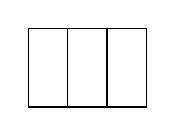
\begin{tikzpicture}[scale=.5]
   \draw (0,0) rectangle (3,2);
   \draw (1,0) -- (1,2);
   \draw (2,0) -- (2,2);
  \end{tikzpicture}
  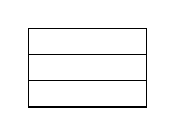
\begin{tikzpicture}[scale=.5]
   \draw (0,0) rectangle (3,2);
   \draw (0,.6666) -- (3,.6666);
   \draw (0,1.3333) -- (3,1.3333);
  \end{tikzpicture}
  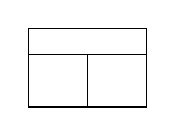
\begin{tikzpicture}[scale=.5]
   \draw (0,0) rectangle (3,2);
   \draw (0,1.3333) -- (3,1.3333);
   \draw (1.5,0) -- (1.5,1.333);
  \end{tikzpicture}
  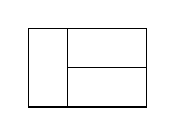
\begin{tikzpicture}[scale=.5]
   \draw (0,0) rectangle (3,2);
   \draw (1,0) -- (1,2);
   \draw (1,1) -- (3,1);
  \end{tikzpicture}

  %\noindent
\includegraphics[width=.45\textwidth, keepaspectratio]{../..//media/cap1/secoes/licao1_atv1.png}
    \item       Cada parte é {\it um terço} da barra ou a {\it terça parte} da barra.
\end{enumerate} %s
\end{resposta*}

\subsection{Atividade 2}

  \noindent {\bf Objetivos específicos: Levar o aluno a} \vspace{.1cm}

\begin{itemize} %s
    \item       Perceber que cada unidade (no caso, uma pizza) pode ser subdividida em um mesmo número de partes sem que cada divisão represente uma equipartição.
    \item       Distinguir uma equipartição dentre partições diversas.
    \item       Diferenciar       ``a divisão da unidade em quatro partes quaisquer'' da       ``divisão da unidade em quatro partes iguais''.
    \item       Compreender as expressões ``um quarto de'' e ``quarta parte de'' como forma de identificar uma das partes da equipartição em 4 partes.
\end{itemize} %s
 \vspace{.1cm}

  \noindent {\bf Recomendações e sugestões para o desenvolvimento da atividade:} \vspace{.1cm}

\begin{itemize} %s
    \item       Recomenda-se que a atividade seja desenvolvida em grupos de 3 a 5 alunos.
    \item       As diversas soluções apresentadas pelos diferentes grupos devem ser discutidas com a turma inteira.
    \item       É possível que os alunos utilizem expressões variadas para nomear as partes de pizzas em cada divisão. Por exemplo,       ``a maior quarta parte'',       ``a menor quarta parte'',       ``as quartas partes iguais entre si'',       ``a menor parte'',       ``a maior parte'', dentre outras. É importante que a discussão conduza os alunos ao entendimento de que apenas as partes da equipartição podem ser chamadas de       ``quartos'' da pizza, as demais são simplesmente fatias ou pedaços, por exemplo.
    \item       Os alunos devem reconhecer que apenas uma das repartições propostas sugere a equipartição, respondendo assim a última questão proposta nesta atividade.
    \item       Essa atividade pode ser adaptada para alunos com deficiência visual. Para isso, sugere-se confeccionar os modelos das três pizzas repartidas, que estão disponíveis para reprodução no final do livro, em três materiais diferentes. Por exemplo, papel comum e papéis com texturas diferentes, tecido ou material emborrachado.
\end{itemize} %s


\begin{resposta*}{Atividade 2}
\begin{enumerate} [a),wide,labelindent=0pt] %d
    \item       Sim. Cada grupo repartiu sua pizza em quatro fatias.
    \item       Não, pois algumas fatias têm quantidades de pizza diferentes das outras.
    \item       Apenas no grupo 1 as 4 crianças receberam a mesma quantidade de pizza. Cada fatia da pizza do grupo 1 é {\it um quarto} da pizza ou {\it a quarta parte} da pizza. Diferentemente das demais pizzas.
\end{enumerate} %d
\end{resposta*}



\subsection{Atividade 3}
  \noindent {\bf Objetivos específicos: Levar o aluno a}\vspace{.1cm}

\begin{itemize} %s
    \item       Abordar a equipartição em um modelo linear.
    \item       Reconhecer a quarta parte como a metade da metade.
\end{itemize} %s
 \vspace{.1cm}

  \noindent {\bf Recomendações e sugestões para o desenvolvimento da atividade:} \vspace{.1cm}

\begin{itemize} %s
    \item       Recomenda-se que esta atividade seja desenvolvida em grupos de quatro alunos.
    \item       Cada grupo deve receber um pedaço de barbante de, aproximadamente, 1m e quatro enfeites (todos iguais).
    \item       Os quatro enfeites precisam ser confeccionados antes da realização da tarefa. Sugerem-se estrelas, cujos modelos estão disponíveis para reprodução no final do livro. No entanto, segundo a avaliação do professor, os enfeites podem ser outros, desde que sejam os 4 congruentes.
    \item       Como sugestão, se possível, solicitar aos alunos que confeccionem os enfeites, por exemplo, associando esta atividade com geometria, com a abordagem de grandezas e medidas, com a disciplina de artes ou envolvendo culturas artesanais populares.
    \item       A equipartição do barbante não deve ser obtida a partir da medida do barbante, mas por sucessivas dobras do barbante sobre ele mesmo, como ilustrado na resposta da atividade. Tal discussão também  será útil na abordagem de frações equivalentes na Lição 4.
    \item       A manipulação e a dobra do barbante devem sustentar a discussão para a identificação da       ``metade da metade'' com a       ``quarta parte'' do barbante. Nesse caso, a identificação se dará pela sobreposição das partes.
\end{itemize} %s

\vspace*{\fill}
\columnbreak

\begin{resposta*}{Atividade 3}

Uma maneira de se cortar o barbante é dobrar ao meio e depois dobrar novamente ao meio, obtendo quatro partes iguais, como ilustrado na figura a seguir.
  \begin{center}
  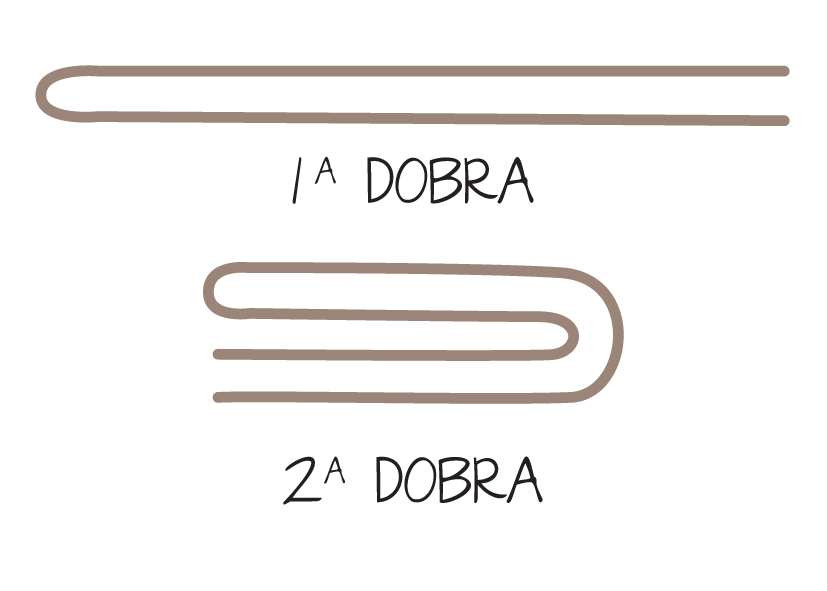
\includegraphics[width=200pt, keepaspectratio]{..//media/cap1/secoes/pngs_licao_01/ativ3_fig03.png}
  \end{center}
\end{resposta*}
\end{multicols}

\subsection{Sobre o Organizando as Ideias}

  Nesta etapa, espera-se que os alunos compreendam as frações como forma de expressar quantidades. O objetivo é que percebam seu papel para expressar quantidades em situações de equipartição da unidade. Assim, as frações podem ser utilizadas no dia a dia para identificar quantidades do mesmo modo que os números naturais, já conhecidos dos alunos. Por exemplo, como nas expressões:   ``dois ovos'',   ``duas xícaras de farinha'',   ``um terço de xícara de cacau'' e   ``meio litro de leite''.

  Objetiva-se a expressão verbal e não a representação simbólica. Espera-se, assim, que os alunos apropriem-se das expressões verbais que identificam as frações unitárias (um meio, um terço, um quarto, ... , um nono e um décimo) antes de serem apresentados formalmente à simbologia matemática (que será objetivo da próxima lição).  A referência às frações unitárias com a expressão   ``um'' antes da identificação da parte, como, por exemplo, em   ``um terço'' e em   ``um sétimo'' é uma decisão pedagógica. Claro que é possível se referir a essas frações simplesmente por   ``terço'' e   ``sétimo'', respectivamente. No entanto, nas próximas seções, pretende-se que as frações não unitárias, como   ``dois terços'' e   ``nove sétimos'', por exemplo, sejam entendidas a partir da justaposição das frações unitárias correspondentes, o que é naturalmente amparado pela contagem. Nas expressões verbais relativas às frações unitárias, o   ``um'' antes da identificação da parte está associado à contagem. Dessa forma, a compreensão das frações   ``um terço'' e   ``dois terços'' ou das frações ``um sétimo'' e ``nove sétimos'', por exemplo, seguem a mesma construção lógica.

\Bg

\begin{multicols}{2}
\subsection{Atividade 4}
  \noindent {\bf Objetivos específicos: Levar o aluno a}\vspace{.1cm}:
\begin{itemize} %s
    \item       Reconhecer que, em uma equipartição, as partes podem não ter a mesma forma.
    \item       Identificar a equivalência entre as partes de uma equipartição a partir de sobreposição ou da comparação pelo reconhecimento da associação a uma mesma fração unitária (no caso, $\frac{1}{4}$).
    \item       Reconhecer a quarta parte como a metade da metade.
\end{itemize} %s
 \vspace{.1cm}

  \noindent {\bf Recomendações e sugestões para o desenvolvimento da atividade:} \vspace{.1cm}

\begin{itemize} %s
    \item       Recomenda-se que esta atividade seja desenvolvida em grupos de 3 a 5 alunos. Cada grupo deve receber as imagens dos oito retângulos, disponíveis para reprodução no final do livro, e colori-las, cada um com uma cor diferente das demais.
    \item       Em cada grupo, os alunos devem decidir qual (ou quais) das divisões propostas para os retângulos correspondem a uma partição em quartos. É importante observar que todos os retângulos estão divididos em quartos.
    \item       Conduza a discussão de modo a levar os alunos a reconhecer que, em uma equipartição, as partes não precisam ter a mesma forma.
    \item       Se necessário, o professor pode associar cada retângulo a um objeto concreto (por exemplo, uma barra de chocolate ou a um pedaço de bolo). No entanto, nesta atividade, espera-se que os alunos consigam lidar com a figura de um retângulo como representativa de uma unidade genérica.
    \item       Recomenda-se que os alunos recortem as partes de cada um dos retângulos para realizar a comparação por sobreposição. No entanto, essa estratégia não será suficiente para todos os 8 casos. Em alguns casos, a comparação se dará pela identificação da fração unitária correspondente a cada parte. Nesses casos, o aluno deve reconhecer que a quarta parte é equivalente à metade da metade. Por exemplo, como no caso seguir.
\end{itemize} %s

\noindent 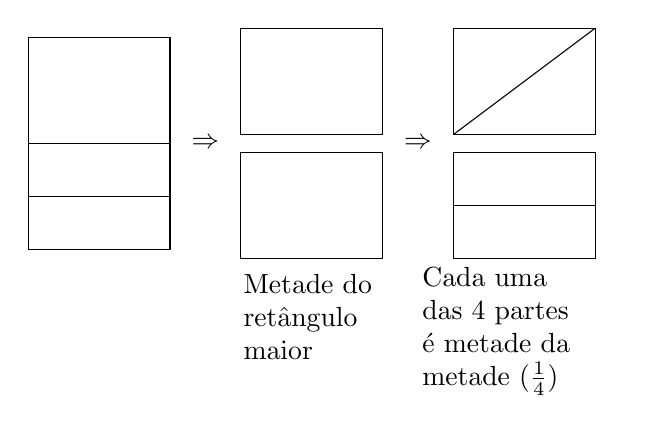
\begin{tikzpicture}[scale=0.45]
  \draw (0,0) rectangle (4,3);
  \draw (0,3) rectangle (4,6);
  \draw (0,1.5) -- (4,1.5);
  \draw (5,3) node{$\Rightarrow$};
  \draw (6,-0.25) rectangle (10,2.75);
  \draw (6,3.25) rectangle (10,6.25);
  \node[text width=2cm]  at (8.3,-1.9) {Metade do retângulo maior};
  \draw (11,3) node{$\Rightarrow$};
  \draw (12,-0.25) rectangle (16,2.75);
  \draw (12,3.25) rectangle (16,6.25);
  \draw (12,3.25) -- (16,6.25);
  \draw (12,1.25) -- (16,1.25);
  \node[text width=2.5cm]  at (13.9,-2.3) {Cada uma das 4 partes é metade da metade ($\frac{1}{4}$)};
  \end{tikzpicture}
\begin{itemize} %s
    \item       Segundo a avaliação do professor, a atividade pode ser realizada em duas etapas. Em um primeiro momento, os alunos recebem as primeiras quatro das oito imagens e realizam a atividade com essas imagens - cuja comparação se dá apenas pela sobreposição. Em seguida, recebem as outras quatro, para concluir a atividade. Para as últimas 4 figuras, será necessário reconhecer a quarta parte como a metade da metade. É importante que o professor, ao final das duas etapas, avalie as escolhas como um todo.
\end{itemize} %s


\begin{resposta*}{Atividade 4}
\begin{enumerate}[a),wide,labelindent=0pt] %s
    \item       Todos os retângulos estão divididos em quartos.
    \item       Dois desenhos possíveis são:

    \begin{tikzpicture}[scale=5, x=1mm, y=1mm]
  \draw[fill=common, fill opacity=.3] (0,0) rectangle (1.5,6);
  \draw[fill=common, fill opacity=.3] (1.5,0) rectangle (2,6);
  \draw[fill=common, fill opacity=.3] (2,0) rectangle (3.5,6);
  \draw[fill=common, fill opacity=.3] (3.5,0) rectangle (4,6);
  \draw[fill=common, fill opacity=.3] (5,0) rectangle (9,3);
  \draw[fill=common, fill opacity=.3] (5,3) rectangle (9,6);
  \draw (5,0) -- (7,3);
  \draw (5,3) -- (9,6);
\end{tikzpicture}
\end{enumerate} %s
\end{resposta*}

\Bg
\end{multicols}
\subsection{Atividade 5}
  \noindent {\bf Objetivos específicos: Levar o aluno a}\vspace{.1cm}:

\begin{itemize} %s
    \item       Identificar uma mesma fração unitária (no caso, a terça parte) em representações diversas, ou seja, em representações de unidades não necessariamente congruentes.
\end{itemize} %s

 \vspace{.1cm}

  \noindent {\bf Recomendações e sugestões para o desenvolvimento da atividade:} \vspace{.1cm}
\begin{itemize} %s
    \item       Recomenda-se que esta atividade seja desenvolvida em grupos de 3 a 5 alunos.
    \item       Durante a discussão, os alunos devem ser estimulados a explicar as suas escolhas. A discussão sobre os motivos da identificação, ou não, de cada uma das representações à terça parte da unidade correspondente será fundamental para atingir o objetivo da atividade.
    \item       Os alunos devem reconhecer que, independente da unidade considerada, em uma equipartição em 3 partes, cada uma das partes é um terço (ou a terça parte) da unidade.
    \item       Aproveite as próprias palavras e os argumentos dos alunos para conduzi-los às conclusões esperadas.
    \item       Fique atento aos alunos que selecionarem as figuras que simplesmente possuem alguma associação com o número 3, não correspondendo a terços. Por exemplo, um aluno que associe a       {\bf Figura i)} a terços pode ainda não ter compreendido a necessidade da equipartição para a identificação de um terço. Já o aluno que associa       {\bf Figura j)}       a terços pode estar simplesmente contando as partes em vermelho, sem que tenha reconhecido que a figura deveria estar dividida em 3 partes iguais e não em 5.
\end{itemize} %s

\begin{resposta*}{Atividade 5}

A parte em vermelho representa um terço da figura nos itens c), d), e), f) e h).
\end{resposta*}

\pagebreak

\subsection{Atividade 6}
  \noindent {\bf Objetivos específicos: Levar o aluno a}\vspace{.1cm}:
\begin{itemize} %d
    \item       Recompor a unidade a partir de uma fração unitária dada em modelos contínuos.
    \item       Relacionar uma fração da unidade à quantidade necessária dessas partes para compor a unidade. Assim, por exemplo, é necessário reunir cinco       {\it quintas partes}       para recompor o todo.
\end{itemize} %d


 \vspace{.1cm}

  \noindent {\bf Recomendações e sugestões para o desenvolvimento da atividade:} \vspace{.1cm}

  \begin{itemize} %d
    \item       Recomenda-se que a atividade seja desenvolvida em grupos de 3 a 5 alunos.
    \item       É importante ter em mente que existem várias soluções para cada item. Por exemplo, o primeiro item pode ser corretamente respondido por:             \begin{tikzpicture}[scale=.2]
\draw [fill=common, fill opacity=.3] (0,0) arc (0:180:3) -- (0,0) -- cycle;
\draw (-3,0) -- (-3,3);
\end{tikzpicture}
 e
 \begin{tikzpicture}[scale=.2]
\draw [fill=common, fill opacity=.3] (0,0) arc (0:90:3) -- (-3,0) -- cycle;
\draw [fill=common, fill opacity=.3] (-3,0) arc (270:180:3) -- (-3,3) -- cycle;
\end{tikzpicture}.
    \item       Avalie a possibilidade de discutir com os estudantes respostas que sejam reuniões de partes não justapostas, por exemplo, no primeiro item pode-se ter também             \begin{tikzpicture}[scale=.2]
\draw [fill=common, fill opacity=.3] (0,0) arc (0:90:3) -- (-3,0) -- cycle;
\draw [fill=common, fill opacity=.3] (3.7,0) arc (0:90:3) -- (0.7,0) -- cycle;
\end{tikzpicture}
      como resposta.
    \item       Estimule os alunos a reconhecer (e a fazer) mais do que uma representação para a unidade em cada item.
    \item       Estimule os alunos a, a partir da identificação da fração unitária, determinar a quantidade de partes necessárias para recompor a unidade.
\end{itemize} %d

\begin{resposta*}{Atividade 6}

Algumas possibilidades de respostas para cada linha da tabela do enunciado estão nas respectivas linhas abaixo.
\begin{center}
% arcos de círculos
 \def \sc {0.22}
 \begin{tabular}{ccc}

\begin{tikzpicture}[scale=\sc]
\draw [fill=common, fill opacity=.3] (0,0) arc (0:180:3) -- (0,0) -- cycle;
\draw (-3,0) -- (-3,3);
\end{tikzpicture}
&
\begin{tikzpicture}[scale=\sc]
\draw [fill=common, fill opacity=.3] (0,0) arc (0:90:3) -- (-3,0) -- cycle;
\draw [fill=common, fill opacity=.3] (-3,0) arc (270:180:3) -- (-3,3) -- cycle;
\end{tikzpicture}

&
\begin{tikzpicture}[scale=\sc]
\draw [fill=common, fill opacity=.3] (0,0) arc (0:90:3) -- (-3,0) -- cycle;
\draw [fill=common, fill opacity=.3] (3.7,0) arc (0:90:3) -- (0.7,0) -- cycle;
\end{tikzpicture}

\\

\begin{tikzpicture}[scale=\sc]
\draw [fill=common, fill opacity=.3] (0,0) arc (0:270:3) -- (-3,0) -- cycle;
\draw (-3,0) -- (-6,0);
\draw (-3,0) -- (-3,3);
\end{tikzpicture}
&

\begin{tikzpicture}[scale=\sc]
\draw [fill=common, fill opacity=.3] (0,0) arc (0:90:3) -- (-3,0) -- cycle;
\draw [fill=common, fill opacity=.3] (-3,0) arc (270:180:3) -- (-3,3) -- cycle;
\draw [fill=common, fill opacity=.3] (-3,0) arc (180:270:3) -- (0,0) -- cycle;
\end{tikzpicture}
 &
\begin{tikzpicture}[scale=\sc]
\draw [fill=common, fill opacity=.3] (0,0) arc (0:90:3) -- (-3,0) -- cycle;
\draw [fill=common, fill opacity=.3] (3.7,0) arc (0:90:3) -- (0.7,0) -- cycle;
\draw [fill=common, fill opacity=.3] (7.4,0) arc (0:90:3) -- (4.4,0) -- cycle;
\end{tikzpicture}
\\

\begin{tikzpicture}[scale=\sc]
\draw [fill=common, fill opacity=.3] (0,0) arc (0:360:3) -- (-3,0) -- cycle;
\draw (-3,0) -- (-6,0);
\draw (-3,0) -- (-3,3);
\draw (-3,0) -- (-3,-3);
\end{tikzpicture}
 &
\begin{tikzpicture}[scale=\sc]
\draw [fill=common, fill opacity=.3] (0,3) arc (90:270:3) -- (0,3) -- cycle;
 \draw [fill=common, fill opacity=.3] (3,3) arc (0:-90:3) -- (0,3) -- cycle;
 \draw [fill=common, fill opacity=.3] (0,0) arc (90:0:3) -- (0,-3) -- cycle;
 \draw  (0,0) -- (-3,0);
\end{tikzpicture}
 &
\begin{tikzpicture}[scale=\sc]
\draw [fill=common, fill opacity=.3] (0,0) arc (0:90:3) -- (-3,0) -- cycle;
\draw [fill=common, fill opacity=.3] (3.7,0) arc (0:90:3) -- (0.7,0) -- cycle;
\draw [fill=common, fill opacity=.3] (7.4,0) arc (0:90:3) -- (4.4,0) -- cycle;
\draw [fill=common, fill opacity=.3] (11.1,0) arc (0:90:3) -- (8.1,0) -- cycle;
\end{tikzpicture}
 \\

\begin{tikzpicture}[scale=\sc]
\draw [fill=common, fill opacity=.3] (0,0) rectangle (3,3);
\draw [fill=common, fill opacity=.3] (3,0) rectangle (6,3);
\end{tikzpicture}
 &
\begin{tikzpicture}[scale=\sc]
\draw [fill=common, fill opacity=.3] (0,0) rectangle (3,3);
\draw [fill=common, fill opacity=.3] (0,3) rectangle (3,6);
\end{tikzpicture}

&
\begin{tikzpicture}[scale=\sc]
\draw [fill=common, fill opacity=.3] (0,0) rectangle (3,3);
\draw [fill=common, fill opacity=.3] (3.7,0) rectangle (6.7,3);
\end{tikzpicture}

\\

\begin{tikzpicture}[scale=\sc]
\draw [fill=common, fill opacity=.3] (0,0) rectangle (3,3);
\draw [fill=common, fill opacity=.3] (3,0) rectangle (6,3);
\draw [fill=common, fill opacity=.3] (6,0) rectangle (9,3);
\end{tikzpicture}
 &
\begin{tikzpicture}[scale=\sc]
\draw [fill=common, fill opacity=.3] (0,0) rectangle (3,3);
\draw [fill=common, fill opacity=.3] (0,3) rectangle (3,6);
\draw [fill=common, fill opacity=.3] (3,0) rectangle (6,3);
\end{tikzpicture}
 &

\begin{tikzpicture}[scale=\sc]
\draw [fill=common, fill opacity=.3] (0,0) rectangle (3,3);
\draw [fill=common, fill opacity=.3] (3,3) rectangle (6,6);
\draw [fill=common, fill opacity=.3] (6,0) rectangle (9,3);
\end{tikzpicture}
\\

\begin{tikzpicture}[scale=\sc]
\draw [fill=common, fill opacity=.3] (0,0) rectangle (3,3);
\draw [fill=common, fill opacity=.3] (3,0) rectangle (6,3);
\draw [fill=common, fill opacity=.3] (6,0) rectangle (9,3);
\draw [fill=common, fill opacity=.3] (9,0) rectangle (12,3);
\end{tikzpicture}
&
\begin{tikzpicture}[scale=\sc]
\draw [fill=common, fill opacity=.3] (0,0) rectangle (3,3);
\draw [fill=common, fill opacity=.3] (0,3) rectangle (3,6);
\draw [fill=common, fill opacity=.3] (3,0) rectangle (6,3);
\draw [fill=common, fill opacity=.3] (3,3) rectangle (6,6);
\end{tikzpicture}
&
\begin{tikzpicture}[scale=\sc]
\draw [fill=common, fill opacity=.3] (0,3) rectangle (3,6);
\draw [fill=common, fill opacity=.3] (0,0) rectangle (3,3);
\draw [fill=common, fill opacity=.3] (3,0) rectangle (6,3);
\draw [fill=common, fill opacity=.3] (6,0) rectangle (9,3);
\end{tikzpicture}
\\

\begin{tikzpicture}[scale=\sc]
\draw  (0,0) -- (3,3) -- (6,0);
\end{tikzpicture}
&
\begin{tikzpicture}[scale=\sc]
\draw  (0,0) -- (3,3);
\draw  (2,0) -- (5,3);
\end{tikzpicture}
 &
\begin{tikzpicture}[scale=\sc]
\draw  (0,0) -- (3,3);
\draw  (3,0) -- (0,3);
\end{tikzpicture}
\\

\begin{tikzpicture}[scale=\sc]
\draw  (0,0) -- (3,3) -- (6,0) -- (9,3);
\end{tikzpicture}
&
\begin{tikzpicture}[scale=\sc]
\draw  (0,0) -- (3,3);
\draw  (2,0) -- (5,3);
\draw  (4,0) -- (7,3);
\end{tikzpicture}
 &
\begin{tikzpicture}[scale=\sc]
\draw  (0,0) -- (3,3);
\draw  (4,0) -- (1,3);
\draw  (2,0) -- (5,3);
\end{tikzpicture}
\\

\begin{tikzpicture}[scale=\sc]
\draw  (0,0) -- (3,3) -- (0,6) -- (-3,3) -- (0,0);
\end{tikzpicture}
&
\begin{tikzpicture}[scale=\sc]
\draw  (0,0) -- (3,3);
\draw  (2,0) -- (5,3);
\draw  (4,0) -- (7,3);
\draw  (6,0) -- (9,3);
\end{tikzpicture}
 &
\begin{tikzpicture}[scale=\sc]
\draw  (0,0) -- (3,3);
\draw  (4,0) -- (1,3);
\draw  (2,0) -- (5,3);
\draw (2,0) -- (-1,3);
\end{tikzpicture}
\\

%triängulos
\begin{tikzpicture}[scale=\sc]
\draw [fill=common, fill opacity=.3] (0,0) -- (3,0) -- (-1.5,1.5) -- cycle;
\draw [fill=common, fill opacity=.3] (3,0) -- (6,0) -- (1.5,1.5) -- cycle;
\end{tikzpicture}

 &
\begin{tikzpicture}[scale=\sc]
\draw [fill=common, fill opacity=.3] (0,0) -- (3,0) -- (-1.5,1.5) -- cycle;
\draw [fill=common, fill opacity=.3] (3,0) -- (-1.5,1.5) -- (1.5,1.5) -- cycle;
\end{tikzpicture}
 &
\begin{tikzpicture}[scale=\sc]
\draw [fill=common, fill opacity=.3] (0,0) -- (3,0) -- (-1.5,1.5) -- cycle;
\draw [fill=common, fill opacity=.3] (0,0) -- (-1.5,1.5) -- (-4.5,1.5) -- cycle;
\end{tikzpicture}
\\


\begin{tikzpicture}[scale=\sc]
\draw [fill=common, fill opacity=.3] (0,0) -- (3,0) -- (-1.5,1.5) -- cycle;
\draw [fill=common, fill opacity=.3] (3,0) -- (6,0) -- (1.5,1.5) -- cycle;
\draw [fill=common, fill opacity=.3] (6,0) -- (9,0) -- (4.5,1.5) -- cycle;
\end{tikzpicture}
&
\begin{tikzpicture}[scale=\sc]
\draw [fill=common, fill opacity=.3] (0,0) -- (3,0) -- (-1.5,1.5) -- cycle;
\draw [fill=common, fill opacity=.3] (3,0) -- (-1.5,1.5) -- (1.5,1.5) -- cycle;
\draw [fill=common, fill opacity=.3] (-1.5,1.5) -- (1.5,1.5) -- (-3,3) -- cycle;
%\draw [fill=common, fill opacity=.3] (1.5,1.5) -- (-3,3) -- (0,3) -- cycle;
\end{tikzpicture}
 &
\begin{tikzpicture}[scale=\sc]
\draw [fill=common, fill opacity=.3] (0,0) -- (3,0) -- (-1.5,1.5) -- cycle;
\draw [fill=common, fill opacity=.3] (0,0) -- (-1.5,1.5) -- (-4.5,1.5) -- cycle;
\draw [fill=common, fill opacity=.3] (-3,0) -- (0,0) -- (-4.5,1.5) -- cycle;
\end{tikzpicture}
\\

\begin{tikzpicture}[scale=\sc]
\draw [fill=common, fill opacity=.3] (0,0) -- (3,0) -- (-1.5,1.5) -- cycle;
\draw [fill=common, fill opacity=.3] (3,0) -- (6,0) -- (1.5,1.5) -- cycle;
\draw [fill=common, fill opacity=.3] (6,0) -- (9,0) -- (4.5,1.5) -- cycle;
\draw [fill=common, fill opacity=.3] (9,0) -- (12,0) -- (7.5,1.5) -- cycle;
\end{tikzpicture}
 &

\begin{tikzpicture}[scale=\sc]
\draw [fill=common, fill opacity=.3] (0,0) -- (3,0) -- (-1.5,1.5) -- cycle;
\draw [fill=common, fill opacity=.3] (3,0) -- (-1.5,1.5) -- (1.5,1.5) -- cycle;
\draw [fill=common, fill opacity=.3] (-1.5,1.5) -- (1.5,1.5) -- (-3,3) -- cycle;
\draw [fill=common, fill opacity=.3] (1.5,1.5) -- (-3,3) -- (0,3) -- cycle;
\end{tikzpicture}
 &
\begin{tikzpicture}[scale=\sc]
\draw [fill=common, fill opacity=.3] (0,0) -- (3,0) -- (-1.5,1.5) -- cycle;
\draw [fill=common, fill opacity=.3] (0,0) -- (-1.5,1.5) -- (-4.5,1.5) -- cycle;
\draw [fill=common, fill opacity=.3] (-3,0) -- (0,0) -- (-4.5,1.5) -- cycle;
\draw [fill=common, fill opacity=.3] (-4.5,1.5) -- (-1.5,1.5) -- (-6,3) -- cycle;
\end{tikzpicture}

\end{tabular}
\end{center}
\end{resposta*}


\pagebreak
\begin{multicols}{2}
\subsection{Atividade 7}

  \noindent {\bf Objetivos específicos: Levar o aluno a}: \vspace{.1cm}

\begin{itemize} %s
    \item       Representar uma fração unitária a partir de uma unidade dada.
    \item       Reconhecer (e obter) um quarto como a metade da metade e um oitavo como a metade de um quarto.
    \item       Comparar as frações unitárias metade, um quarto e um oitavo de um mesmo quadrado.
\end{itemize} %s

 \vspace{.1cm}

  \noindent {\bf Recomendações e sugestões para o desenvolvimento da atividade:} \vspace{.1cm}

  \begin{itemize} %s
    \item       Esta é uma atividade que o aluno pode fazer individualmente.
    \item       Não se espera que, nesta atividade, os alunos usem a medida para fazer a equipartição de maneira mais precisa. O objetivo é fazer a equipartição livremente e de forma coerente. Assim, por exemplo, podem ser aceitas como respostas:
\end{itemize} %s
\begin{center}
\begin{tikzpicture}[scale=.7]
 \draw[fill=common, fill opacity=.3] (0,0) rectangle (3,3);
 \draw[decorate, decoration={snake, amplitude= .2 mm}] (1.5,0) -- (1.5,3);
\end{tikzpicture}
e
\begin{tikzpicture}[scale=.7]
 \draw[fill=common, fill opacity=.3] (0,0) rectangle (3,3);
 \draw[decorate, decoration={snake, amplitude= .2 mm}] (0,0) -- (3,3);
\end{tikzpicture}
\end{center}
  Já as representações a seguir sugerem que os alunos precisam revisar os conceitos exigidos para a solução da atividade:
\begin{center}
  \begin{tikzpicture}[scale=.7]
 \draw[fill=common, fill opacity=.3] (0,0) rectangle (3,3);
 \draw[decorate, decoration={snake, amplitude= .2 mm}] (2.3,0) -- (2.3,3);
\end{tikzpicture}
\end{center}
\begin{itemize} %s
    \item       A representação da unidade se dá de forma genérica por um quadrado.
    \item       Espera-se que os alunos reconheçam que para obter um quarto da unidade basta tomar a metade da metade. E que, para determinar um oitavo pode dividir um quarto ao meio.
    \item       Recomende que os alunos usem dobradura para identificar as frações pedidas. Assim, por exemplo, a fração       $\frac{1}{4}$       pode ser obtida por duas dobras do papel.
    \item       Discuta com os estudantes que quanto maior o número de partes iguais em que se particiona o quadrado, menor fica cada uma das partes.
    \item       Procure apresentar e discutir com a turma mais do que uma solução para cada item.
    \item             {\bf As diferentes soluções apresentadas pelos alunos podem enriquecer a discussão}. A comparação entre, por exemplo, a metade do quadrado proveniente da dobradura pela diagonal e o quarto do quadrado proveniente da dobradura a partir de linhas paralelas aos lados (como um sinal de       ``$+$'') pode não ser tão natural. Dificuldade semelhante pode ser observada na comparação entre esse mesmo quarto do quadrado e o oitavo do quadrado proveniente de uma sequência de dobraduras paralelas a um dos lados, determinando       ``faixas paralelas''. Nesses casos, para executar a comparação, é necessário que os alunos reconheçam partes de formatos diferentes que correspondem a uma mesma fração do quadrado como iguais em quantidade. Assim, a comparação entre a metade do quadrado, obtida pela dobradura na diagonal, e o quarto do quadrado, obtido pela dobraduta       ``em sinal de $+$'', pode ser amparada pelo reconhecimento de que a metade em questão é igual em quantidade à metade do quadrado obtida por uma única dobra paralela a um dos lados, que é o dobro do quarto do quadrado.
\end{itemize} %s

\begin{resposta*}{Atividade 7}

  Algumas soluções possíveis, convencionais e outras menos convencionais são:

        \begin{enumerate}[a)]
         \item Metade:   \newline
        \begin{tikzpicture}[scale=.8]
         \draw[fill=common, fill opacity=.3] (0,0) rectangle (2,2);
         \draw[fill=attention] (0,1) rectangle (2,2);
        \end{tikzpicture}
        \begin{tikzpicture}[scale=.8]
         \draw[fill=common, fill opacity=.3] (0,0) rectangle (2,2);
         \draw[fill=attention] (0,0) -- (2,2) -- (0,2)--cycle;
        \end{tikzpicture}
        \begin{tikzpicture}[scale=.8]
         \draw[fill=common, fill opacity=.3] (0,0) rectangle (2,2);
         \draw[fill=attention] (0,2) -- (2,2) -- (1,1)--cycle;
         \draw[fill=attention] (0,0) -- (2,0) -- (1,1)--cycle;
        \end{tikzpicture}
        \begin{tikzpicture}[scale=.8]
         \draw[fill=common, fill opacity=.3] (0,0) rectangle (2,2);
         \draw[fill=attention] (0,1) rectangle (1,2);
         \draw[fill=attention] (1,0) rectangle (2,1);
        \end{tikzpicture}
       \item Um quarto:  \newline
       \begin{tikzpicture}[scale=.8]
         \draw[fill=common, fill opacity=.3] (0,0) rectangle (2,2);
         \draw[fill=attention] (0,0) rectangle (.5,2);
         \foreach \x in {1,1.5} \draw (\x,0) -- (\x,2);
       \end{tikzpicture}
       \begin{tikzpicture}[scale=.8]
         \draw[fill=common, fill opacity=.3] (0,0) rectangle (2,2);
         \draw[fill=attention] (0,1) rectangle (1,2);
         \draw (1,0) -- (1,1);
         \draw (1,1)-- (2,1);
        \end{tikzpicture}
        \begin{tikzpicture}[scale=.8]
         \draw[fill=common, fill opacity=.3] (0,0) rectangle (2,2);
         \draw[fill=attention] (0,0) -- (1,1) -- (0,2)--cycle;
         \draw (1,1) -- (2,2);
         \draw (1,1) -- (2,0);
        \end{tikzpicture}
        \begin{tikzpicture}[scale=.8]
         \draw[fill=common, fill opacity=.3] (0,0) rectangle (2,2);
         \draw[fill=attention] (2,2) -- (1,2) -- (1,1)--cycle;
         \draw[fill=attention] (0,0) -- (1,0) -- (1,1)--cycle;
         \draw (0,2) -- (2,0);
        \end{tikzpicture}
       \item  Um oitavo:  \newline
       \begin{tikzpicture}[scale=.8]
         \draw[fill=common, fill opacity=.3] (0,0) rectangle (2,2);
         \draw[fill=attention] (0,0) rectangle (.25,2);
         \foreach \x in {.5,.75,...,1.75} \draw (\x,0) -- (\x, 2);
       \end{tikzpicture}
       \begin{tikzpicture}[scale=.8]
         \draw[fill=common, fill opacity=.3] (0,0) rectangle (2,2);
         \draw[fill=attention] (0,1) rectangle (.5,2);
         \draw (0,1)--(2,1);
         \foreach \x in {.5,1,...,1.5} \draw (\x,0) -- (\x,2);
        \end{tikzpicture}
        \begin{tikzpicture}[scale=.8]
         \draw[fill=common, fill opacity=.3] (0,0) rectangle (2,2);
         \draw[fill=attention] (0,1) -- (1,1) -- (0,2)--cycle;
         \draw (0,0) -- (1,1);
        \end{tikzpicture}
        \begin{tikzpicture}[scale=.8]
         \draw[fill=common, fill opacity=.3] (0,0) rectangle (2,2);
         \draw[fill=attention] (2,2) -- (1,2) -- (1,1)--cycle;
         \draw (1,1) -- (1,0);
         \draw (0,0) -- (1,1);
         \end{tikzpicture}
       \item  Dentre as opções apresentadas, a maior fração do quadrado é metade.
        \end{enumerate}
\end{resposta*}

\subsection{Atividade 8}

  \noindent {\bf Objetivos específicos: Levar o aluno a}: \vspace{.1cm}

\begin{itemize} %s
    \item       Representar uma fração unitária (no caso, um meio ou metade) a partir de uma unidade dada.
    \item       Estabelecer representações diferentes para a mesma fração unitária e para uma mesma unidade.
\end{itemize} %s
 \vspace{.1cm}

  \noindent {\bf Recomendações e sugestões para o desenvolvimento da atividade:} \vspace{.1cm}

\begin{itemize} %s
    \item       Essa é uma atividade que o aluno pode fazer individualmente.
    \item       Como na atividade anterior, não se espera que, nesta atividade, o aluno use a medida para fazer a equipartição de maneira mais precisa. O objetivo é que o aluno faça a equipartição livremente e de forma coerente.
    \item       Incentive os alunos a usar dobradura para decidir sobre as diferentes formas de identificar metades na unidade apresentada.
\end{itemize} %s

Observe que a representação da unidade se dá de forma genérica, ainda em modelo contínuo, por uma figura não tradicional como retângulos e círculos, que é determinada pela justaposição de dois hexágonos regulares.

\begin{itemize} %s
    \item       Procure apresentar e discutir com a turma mais do que uma solução para cada item.
\end{itemize} %s

\begin{resposta*}{Atividade 8}

Algumas das respostas possíveis para este problema são:
\begin{center}
\begin{tikzpicture}[scale=.4]
\draw[fill=attention] (3.,5.) -- (3.,3.) -- (4.7,2.) -- (6.46,3.) -- (6.46,5.) -- (4.73,6.) -- cycle;
\draw[fill=common, fill opacity=.3] (6.46,5.) -- (6.46,3.) -- (8.2,2.) -- (9.9,3.) -- (9.9,5.) -- (8.2,6.) -- cycle;
\end{tikzpicture}\hspace{.2cm}
\begin{tikzpicture}[scale=.4]
\draw[fill=common, fill opacity=.3] (3.,5.) -- (3.,3.) -- (4.7,2.) -- (6.46,3.) -- (6.46,5.) -- (4.73,6.) -- cycle;
\draw[fill=common, fill opacity=.3] (6.46,5.) -- (6.46,3.) -- (8.2,2.) -- (9.9,3.) -- (9.9,5.) -- (8.2,6.) -- cycle;
\draw[fill=attention] (4.732050807568877,6.) -- (3.,5.) -- (3.,3.) -- (4.732050807568877,2.) -- cycle;
\draw[fill=attention] (8.2,6.) -- (8.2,2.) -- (9.9,3.) -- (9.9,5.) -- cycle;
\end{tikzpicture}

\begin{tikzpicture}[scale=.4]
\draw[fill=common, fill opacity=.3] (3.,5.) -- (3.,3.) -- (4.7,2.) -- (6.46,3.) -- (6.46,5.) -- (4.73,6.) -- cycle;
\draw[fill=common, fill opacity=.3] (6.46,5.) -- (6.46,3.) -- (8.2,2.) -- (9.9,3.) -- (9.9,5.) -- (8.2,6.) -- cycle;
\draw[fill=attention] (3.,4.) -- (3.,3.) -- (4.732050807568877,2.) -- (6.464101615137757,3.) -- (8.196152422706634,2.) -- (9.928203230275509,3.) -- (9.928203230275509,4.) -- cycle;
\end{tikzpicture}\hspace{.2cm}
\begin{tikzpicture}[scale=.4]
\draw[fill=common, fill opacity=.3] (3.,5.) -- (3.,3.) -- (4.7,2.) -- (6.46,3.) -- (6.46,5.) -- (4.73,6.) -- cycle;
\draw[fill=common, fill opacity=.3] (6.46,5.) -- (6.46,3.) -- (8.2,2.) -- (9.9,3.) -- (9.9,5.) -- (8.2,6.) -- cycle;
\draw[fill=attention] (3,5) -- (3.,3.) -- (4.73,2.) -- (6.46,3.) -- (8.2,2.) -- (9.9,3.) -- cycle;
\end{tikzpicture}
\end{center}
\end{resposta*}




\subsection{Atividade 9}
  \noindent {\bf Objetivos específicos: Levar o aluno a}: \vspace{.1cm}

\begin{itemize} %s
    \item       Reconhecer a metade de uma unidade pela reunião de partes menores e em partições diversas.
    \item       Estabelecer representações diferentes para a mesma fração unitária para uma mesma unidade.
\end{itemize} %s

 \vspace{.1cm}

  \noindent {\bf Recomendações e sugestões para o desenvolvimento da atividade:} \vspace{.1cm}

  \begin{itemize} %s
    \item       Esta é uma atividade que o aluno pode fazer individualmente.
    \item       Esta atividade pretende levar o aluno a perceber que a metade de uma unidade pode ser considerada e identificada mesmo sem que se tenha uma divisão em duas partes iguais.
    \item       Como nas atividades anteriores, não se espera que o aluno use a medida para confirmar a metade da unidade. O objetivo é que o aluno identifique a representação da metade (ou não) por sobreposição e justaposição das partes, decompondo e recompondo a figura.
    \item       Cada aluno deve receber as imagens das figuras, disponíveis para reprodução no final do livro para que possa manipular como achar melhor e conduzir a sua decisão.
    \item       Incentive os alunos a argumentar, justificando a sua decisão. Para isso, podem, por exemplo, se apoiar em dobraduras ou em recortes das partes da figura.
    \item       Procure apresentar e discutir com a turma mais do que uma solução para cada item.
\end{itemize} %s

\begin{resposta*}{Atividade 9}

  As figuras que correspondem à metade da unidade são as de números 1, 2, 4, 5, 6, 8, 9, 11 e 12.
\end{resposta*}

\subsection{Atividade 10}

\noindent {\bf Objetivos específicos: Levar o aluno a}:
\begin{itemize}
 \item Distinguir frações unitárias a partir de representações em modelos de área circular.
\item     Comparar frações unitárias a partir de representações em modelos de área circular.
\end{itemize}

 \vspace{.1cm}

\noindent {\bf Recomendações e sugestões para o desenvolvimento da atividade:} \vspace{.1cm}

\begin{itemize}
 \item Recomenda-se que esta atividade seja desenvolvida em grupos de 3 a 5 alunos. No entanto, cada aluno deve ter o seu próprio material (Círculos de Frações) para realizar a atividade.
 \item   Durante a discussão, os alunos devem ser estimulados a explicar as suas escolhas. A discussão sobre os motivos da identificação, ou não, de cada uma das representações às frações da unidade correspondentes será fundamental para atingir o objetivo da atividade.
 \item    Esta atividade é planejada para ser desenvolvida a partir de material concreto baseado em modelos de área circular. Mais especificamente com um material conhecido como ``Círculos de Frações''. Para aplicá-la, é necessário reproduzir esse material, que está disponível nas páginas para reprodução.
    \item Sendo um material concreto, os círculos de frações têm o papel de auxiliar na visualização da representação das frações, mais especificamente, das frações unitárias.
    \item Na versão utilizada nesta atividade, o círculo corresponde à unidade, ou seja, ao 1 e os setores circulares, diferenciados por cores, correspondem às frações unitárias um meio, um terço, um quarto, um sexto, um sétimo, um oitavo, um nono e um décimo.
    \item Os Círculos de Frações também podem ser utilizados para trabalhar com as frações unitárias, bem como para abordar outros conceitos e assuntos como, por exemplo, frações em geral, comparação de frações ou as operações com frações (adição e subtração).
    \item Refira-se ao círculo inteiro (na cor preta) como círculo ou unidade, e não como todo. Refira-se a cada setor circular como fração do círculo, parte do círculo ou, simplesmente, peça da cor x.
    \item Antes de solicitar aos alunos que realizem a atividade, explore o material ressaltando especialmente o fato de que, reunidas, as peças de uma mesma cor determinam um círculo congruente ao preto.
    \item Ainda antes de solicitar aos alunos que realizem a atividade, explore também o material com perguntas dirigidas a toda a turma como as seguintes: ``Quantas peças azuis cobrem o círculo preto?'' ou ``Quantas peças verdes cobrem o círculo preto?''.
    \item Faça uso do material concreto para ilustrar e explicar a resposta de cada item e incentive os seus alunos a fazerem o mesmo.
    \item Espera-se que a explicação para as respostas, nos oito primeiros itens desta questão, seja a partir da contagem dos setores circulares correspondentes às frações envolvidas. Assim, por exemplo, a resposta do item b) pode ser justificada pelo fato de que são necessários 4 partes de círculo na cor vermelha para compor um círculo preto.
    \item Já para os cinco itens que tratam da comparação, espera-se que os alunos identifiquem os setores que representam as frações envolvidas e procedam a comparação pela sobreposição das peças correspondentes. Assim, por exemplo, a resposta do item l) pode ser justificada pela sobreposição das peças das cores verde e amarelo.
    \item Aproveite a correção desses últimos itens para explorar, a partir dos Círculos de Frações, a relação entre a quantidade de peças de cada cor e o tamanho das peças, ou seja, a relação inversa entre a quantidade de partes em que círculo (unidade) está dividido e o tamanho de cada parte.
\end{itemize}

\end{multicols}


\begin{resposta*}{Atividade 10}
\begin{enumerate}[a)]
 \item Uma peça da cor AZUL é igual a um terço do círculo preto.
 \item    Uma peça da cor VERMELHA é igual a um quarto do círculo preto.
 \item    Uma peça da cor AMARELA é igual a um sétimo do círculo preto.
 \item    Uma peça da cor LARANJA é igual a um nono do círculo preto.
 \item    Uma peça da cor roxa é igual a UM SEXTO do círculo preto.
 \item    Uma peça da cor cinza é igual a UM OITAVO do círculo preto.
 \item    Uma peça da cor branca é igual a UM DÉCIMO do círculo preto.
 \item    Uma peça da cor rosa é igual à METADE do círculo preto.
 \item    Um terço do círculo preto é maior do que um sétimo do círculo preto.
 \item    Um nono do círculo preto é menor do que um quarto do círculo preto.
 \item    Um sétimo do círculo preto é menor quinto do círculo preto.
 \item    Um quarto do círculo preto é maior do que um oitavo do círculo preto.
 \item    Um sexto do círculo preto é maior do que um sétimo do círculo preto
\end{enumerate}

\end{resposta*}

\subsection{Atividade 11}
  \noindent {\bf Objetivos específicos: Levar o aluno a} \vspace{.1cm}

\begin{itemize} %s
    \item       Conhecer e compreender as expressões correspondentes as frações unitárias com denominadores de 5 a 10.
    \item       Comparar frações da unidade através da representação visual de frações do círculo.
    \item Reconhecer a relação inversa entre o número de partes e o tamanho de cada parte.
\end{itemize} %s
 \vspace{.1cm}

  \noindent {\bf Recomendações e sugestões para o desenvolvimento da atividade:} \vspace{.1cm}

  \begin{itemize} %s
    \item       Esta atividade pode ser resolvida individualmente, mas é essencial que seja discutida com toda a turma.
    \item       É provável que nem todos os alunos conheçam ou intuam as expressões correspondentes às frações propostas. Nesse caso, cabe ao professor apresentá-las e diferenciá-las.
    \item       Aproveite esta atividade para revisar e discutir o vocabulário que é objetivo nesta seção:       {\it unidade,}             {\it metade,}             {\it um meio,}             {\it um terço,}             {\it terça parte,}             {\it um quarto,}             {\it quarta parte,}             {\it um quinto,}             {\it quinta parte,}             {\it um sexto,}             {\it sexta parte,}             {\it um sétimo,}             {\it sétima parte,}             {\it um oitavo,}             {\it oitava parte,}             {\it um nono,}             {\it nona parte,}             {\it um décimo}       e       {\it décima parte}      .
\end{itemize} %s

\begin{resposta*}{Atividade 11}
\begin{enumerate}[a),wide,labelindent=0pt] %s
    \item       A correspondência adequada é:
\begin{enumerate} [\;\; I), labelindent=0pt] %d
        \item           A esta afirmação corresponde a figura G).
        \item           A esta afirmação corresponde a figura D).
        \item           A esta afirmação corresponde a figura I).
        \item           A esta afirmação corresponde a figura B).
        \item           A esta afirmação corresponde a figura A).
        \item           A esta afirmação corresponde a figura F).
\end{enumerate} %d

    \item       As frações um sétimo, um oitavo, um nono e um décimo do círculo são menores que um sexto do círculo. Qualquer uma delas está correta.
    \item       As frações um meio, um terço, um quarto, um quinto, um sexto, um sétimo e um oitavo do círculo são maiores que um nono do círculo. Qualquer uma delas está correta.
    \item       As frações um sétimo e um oitavo do círculo são menores que um sexto e maiores que um nono do círculo.
\end{enumerate} %s
\end{resposta*}

\newpage

\subsection{Atividade 12}

  \noindent {\bf Objetivos específicos: Levar o aluno a}: \vspace{.1cm}

\begin{itemize} %s
    \item       Distinguir frações unitárias a partir de representações em modelos diversos, baseados em equipartição ou não.
    \item       Comparar frações unitárias a partir de representações em modelos diversos, baseados em equipartição ou não.
    \item       Estabelecer a comparação entre as frações       ``um meio'',       ``um quarto'' e       ``um décimo''.
    \item       Reconhecer e diferenciar a representação das frações       ``um meio'',       ``um quarto'' e       ``um décimo'' em modelos diversos, baseados em equipartição ou não.
    \item       Estabelecer a comparação entre as frações       ``um meio'',       ``um quarto'' e       ``um décimo''.
\end{itemize} %s

 \vspace{.1cm}

  \noindent {\bf Recomendações e sugestões para o desenvolvimento da atividade:} \vspace{.1cm}

\begin{itemize} %s
    \item       Esta é uma atividade que o aluno pode fazer individualmente.
    \item       Esta atividade pretende levar o aluno a perceber que a metade de uma unidade pode ser considerada e identificada mesmo sem que se tenha uma divisão em duas partes iguais.
    \item       Como nas atividades anteriores, não se espera que os alunos usem a medida para confirmar a metade. O objetivo é que identifiquem a representação da metade (ou não) por sobreposição e justaposição dessas partes, decompondo e recompondo a figura.
    \item       Cada aluno deve receber as imagens das figuras, disponíveis para reprodução no final do livro para que possa manipular como achar melhor e conduzir a sua decisão.
    \item       Incentive os alunos a argumentar, justificando a sua decisão. Para isso, podem, por exemplo, se apoiar em dobraduras ou no recorte das partes da figura.
    \item       Procure apresentar e discutir com a turma mais do que uma solução para cada item
\end{itemize} %s


\begin{resposta*}{Atividade 12}

\begin{tabular}{lll}
a) um meio,&  b) um décimo,& c) um quarto,\\
d) um quarto,& e) um quarto,& f) um meio,\\
g) um quarto,& h) um décimo,& i) um quarto,\\
j) um décimo,& l) um quarto,& m) um meio
\end{tabular}
\end{resposta*}

\clearpage

\noindent {\color{special}{\Large \bf LIÇÃO 2 - Para o professor}}
\vspace{.5cm}

Na Lição anterior, as frações unitárias permitiram reconhecer e registrar quantidades menores que a unidade: meio, um terço, um quarto, etc. Nesta, serão abordadas as frações em geral: as que representam quantidades menores do que a unidade, quantidades maiores do que a unidade ou quantidades inteiras. Também serão introduzidas a notação simbólica de frações e a comparação entre frações de mesmo denominador. 

As frações com numerador diferente de 1 são apresentadas \textbf{reunindo-se (por contagem ou por justaposição) cópias de uma mesma fração unitária.}
Cabe ressaltar que reunir aqui não tem como objetivo tratar da operação de adição, ou seja, não se espera que o aluno compreenda, nem que seja apresentado a ele, $2/3$ como $1/3 + 1/3$. Espera-se no entanto que o raciocínio aditivo, elementar na contagem, ampare a compreensão do aluno.

Para isso, tem-se a representação pictórica como um apoio importante.
Na Atividade 1, as imagens das pizzas amparam a compreensão das frações três quartos, cinco sextos e cinco oitavos como a reunião de cópias de frações unitárias correspondentes à quarta parte, à sexta parte e à oitava parte de uma pizza, respectivamente. Nesse sentido, nas primeiras atividades, há um esforço deliberado para que o estudante faça uso da linguagem de frações apresentada na Lição 1 para expressar frações não unitárias.
Na Atividade 2, as imagens da barra de chocolate amparam a compreensão da fração dois terços como a reunião de duas partes correspondentes à terça parte (ou à fração um terço) de uma barra de chocolate.
Na Atividade 3, sabendo que uma das cinco fatias iguais em que foi repartida uma torta é um quinto da torta, espera-se que o aluno use a linguagem ``dois quintos'' ou ``dois um quintos'' da torta para se referir às outras duas fatias.
Dessa forma, ``dois quintos'' da torta são obtidos pela reunião de duas partes correspondentes a ``um quinto'' da torta.
O objetivo é que esse processo se estenda para a compreensão das frações não unitárias.
Assim, as frações ``quatro quintos'' e ``seis quintos'' são entendidas como a reunião de ``quatro um quintos'' e ``seis um quintos'' da mesma unidade, respectivamente. O processo de reunir frações unitárias pode ser observado como uma contagem (com justaposição ou não) em que a fração unitária tem o papel de unidade na contagem. A fração unitária é uma subunidade da unidade considerada. 

Um cuidado especial recomendado ao professor é com as frações que representam uma quantidade maior que a unidade, introduzidas logo nas primeiras atividades ainda sem notação simbólica. Não é indicado atrasar muito a introdução deste tipo de fração porque o estudante pode fixar-se na ideia de que não há fração maior do que a unidade  (por exemplo, a fração quatro terços pode não fazer sentido para o estudante porque, para ele, não faz sentido dividir uma torta em 3 pedaços e tomar 4). Decidiu-se omitir as terminologias ``fração própria'', ``fração imprópria'' e ``fração aparente'' por se acreditar que esta linguagem não só é desnecessária para a aprendizagem do assunto como também por poder desviar a atenção dos conceitos que realmente importam.
A representação de frações maiores que a unidade na forma de número misto também não é adotada neste texto. Esse tipo de representação não tem um uso que justifique a abordagem nesta etapa da aprendizagem.

Apesar de esta lição introduzir a linguagem simbólica de frações, o estudante talvez ainda precise de uma unidade concreta explícita para dar um significado para a fração $\frac{a}{b}$: por exemplo, ``$\frac{a}{b}$ de uma pizza'' ou ``$\frac{a}{b}$ de uma barra de chocolate''. Apenas na próxima lição, a fração $\frac{a}{b}$ será tratada como número, requerendo a abstração que o conceito de número exige.
\vspace{.15cm}

\noindent OBJETIVOS ESPECÍFICOS DA LIÇÃO 2:
\vspace{.15cm}

\noindent O aluno deve ser capaz de:
\begin{itemize}
 \item  Reconhecer a necessidade de apresentar uma expressão verbal que identifique a quantidade correspondente à junção de duas ou mais partes correspondentes às frações unitárias de mesmo denominador.
 \item  Reconhecer frações não unitárias como a reunião de cópias de frações unitárias de uma mesma unidade. 
 \item  Utilizar as linguagens verbal e simbólica para referir-se a uma fração $\frac{a}{b}$.
 \item  Reconhecer e nomear os termos de uma fração (numerador e denominador). 
 \item  Comparar frações de mesmo denominador.
 \item Reconhecer o papel da unidade na identificação da fração, tanto em situações em  que uma mesma fração pode representar quantidades diferentes como em situações em que frações diferentes podem representar uma mesma quantidade.
\end{itemize}


\pagebreak

%\begin{multicols}{2}
\begin{objetivos}[code={\setcounter{tcb@cnt@objetivos}{0}}]{}{}  %o comando entre colchetes reinicia a numeração dos objetivos manualmente do zero.
  \begin{itemize} %s
\item Estender o conceito de frações para expressar quantidades que correspondam a mais do que uma fração unitária, a partir da junção de duas ou mais partes correspondentes às frações unitárias de mesmo denominador.
\item Reconhecer a necessidade de apresentar uma expressão verbal que identifique a quantidade correspondente à junção de duas ou mais partes correspondentes às frações unitárias de mesmo denominador.
  \end{itemize} %s
\end{objetivos}

\begin{orientacoes}
  \begin{itemize} %s
\item Recomenda-se que a atividade seja realizada individualmente e que os alunos compartilhem suas respostas. 
\item É possível que os alunos utilizem expressões variadas para nomear as quantidades de pizza que cada amigo comeu. Por exemplo, ``três de quatro fatias'', ``três fatias de um quarto de pizza'', ``três quartos de pizza'', dentre outras. É importante que a discussão conduza os alunos ao uso de quartos, sextos e oitavos: ``três quartos'', ``cinco sextos'', ``cinco oitavos'', etc. 
\end{itemize} %s
\end{orientacoes}
%  \noindent {\bf Classificações:}\vspace{.1cm}
% \begin{itemize} %s
%     \item       Heid et al.: Conceito: identificar e descrever
%     \item       Nicely, Jr.: Nível 1: reconhecer
%     \item       UERJ: Observar: identificar e reconhecer
% \end{itemize} %s

\begin{solucao}[code={\setcounter{tcb@cnt@solucao}{0}}]{}{}
\begin{enumerate} [\quad a)] %d
\item Da esquerda para a direita as pizzas são de João, Mariele e Luiza.
\item Na pizza de João uma fatia representa um sexto da pizza. \newline
  Na pizza de Mariele uma fatia representa um oitavo da pizza. \newline
  Na pizza de Luiza uma fatia representa um quarto da pizza.
\item João comeu quatro sextos de sua pizza; Mariele, seis oitavos; e Luiza comeu três quartos de sua pizza.
\end{enumerate} %d
\end{solucao}
\vfill

  \begin{objetivos}{}{}
  \begin{itemize} %s
    % \item Estender o uso de frações para expressar quantidades que correspondam a mais do que uma fração unitária, a partir da justaposição de duas ou mais partes correspondentes às frações unitárias de mesmo denominador.
    % \item Reconhecer e usar frações para expressar quantidades que correspondam a mais do que uma fração unitária, em situação de equipartição de mais do que uma unidade (no caso, duas).
    \item Reconhecer a necessidade de apresentar uma expressão verbal que identifique a quantidade correspondente à junção de duas ou mais partes correspondentes às frações unitárias de mesmo denominador.
    % \item Compreender e usar a expressão ``$n$ terços de''como forma de registrar as $n$ partes da equipartição da unidade em três partes (no caso, dois terços).
    % \item Identificar a fração ``$n$ terços de'' em uma situação de equipartição de mais do que uma unidade.
\item Compreender e usar as expressões ``dois terços'', ``três terços'' e ``quatro terços'' como forma de registrar as duas, três ou quatro partes de uma equipartição da unidade em três partes.
  \end{itemize} %s
\end{objetivos}
\newpage

\begin{orientacoes}
\begin{itemize} %s
   \item Recomenda-se que a atividade seja desenvolvida em grupos de 3 a 5 alunos.
   \item Nesta atividade, é importante que os alunos possam ter cópias de figuras ilustrativas das barras de chocolate para dividir e poder avaliar e decidir as suas respostas. Faça cópias das páginas para reprodução.
   \item A opção por um problema de divisão em partes iguais (dois terços corresponde ao resultado da divisão de 2 unidades em 3 partes iguais) no lugar da abordagem ``parte-todo'' (dois terços corresponde a duas partes da equipartição da unidade em três partes) que, no Brasil, costuma ser o mais tradicional, tem duas justificativas: (1) manter a abordagem que marca a lição anterior: equipartição (agora com múltiplas cópias da unidade); (2) amparar a compreensão de frações cujo numerador é maior do que o denominador pela reunião de cópias de partes da unidade (uma vez que pode não parecer coerente nomear uma parte ``maior do que o todo'').
   \item As diversas soluções apresentadas pelos diferentes grupos devem ser discutidas com a turma inteira.
   \item É possível que os alunos utilizem expressões variadas para nomear as partes dos chocolates em cada divisão e para a quantidade de chocolate que cada irmão recebeu. Por exemplo, ``dois dos seis pedaços'', ``dois pedaços de um terço de chocolate''. É importante que a discussão conduza os alunos ao uso de terços:       ``dois terços'', ``quatro terços'', ``seis terços'', etc. Observa-se que o uso de ``sextos'' muito provavelmente indica uma confusão do aluno em relação ao reconhecimento da unidade.
  
\end{itemize} %s

%  \noindent {\bf Classificações:}\vspace{.1cm}
% \begin{itemize} %s
%     \item       Heid et al.: Conceito: identificar e descrever
%     \item       Nicely, Jr.: Nível 1: reconhecer
%     \item       UERJ: Observar: identificar e reconhecer
% \end{itemize} %s
\end{orientacoes}

\begin{solucao}{}{}
\begin{enumerate} [\quad a)] %d
    \item  Um terço.
    \item  Sim, pois a divisão foi justa no sentido de cada irmã ter recebido a mesma quantidade de chocolate.
    \item  Sim, pois cada irmã recebeu dois pedaços que equivalem, cada um, a um terço de uma barra de chocolate.
    \item  Dois terços de uma barra.
    \item  Três terços de uma barra, ou seja, uma barra inteira de chocolate.
    \item  Quatro terços de uma barra, ou seja, uma barra inteira e um terço de chocolate.
\end{enumerate} %d

\end{solucao}

\newpage

\begin{multicols}{2}
\begin{objetivos}{}{}
  \begin{itemize} %s
\item Reconhecer a necessidade de apresentar uma expressão verbal que identifique a quantidades correspondentes a $n$ quintos.
\item Compreender e usar a expressão ``$n$ quintos de'' como uma forma de identificar a quantidade equivalente a $n$ partes da equipartição da unidade em quintos, incluindo os casos em que $n$ é maior do que cinco.
\item Comparar frações de mesmo denominador em uma situação.
\end{itemize} %s
\end{objetivos}

\begin{orientacoes}
  \begin{itemize} %s
  \item       Recomenda-se que a atividade seja desenvolvida em grupos de 3 a 5 alunos.
  \item       Nesta atividade, é importante que os alunos possam ter cópias de figuras ilustrativas da torta para dividir e poder avaliar e decidir suas respostas. Faça cópias das páginas para reprodução e entregue uma para cada grupo.
  \item       As diversas soluções apresentadas pelos diferentes grupos devem ser discutidas com a turma inteira.
  \item       Em particular, no Item a), não se espera, nem se recomenda, que a representação feita pelos alunos seja amparada por medida. O objetivo é que façam a equipartição livremente e de forma coerente. Assim, por exemplo, pode ser aceita como resposta a solução indicada na figura a seguir.


\begin{center}
 \begin{tikzpicture}[yscale=.45,xscale=.4, x=1mm,y=1mm, rotate=90]
 \draw (0,0) rectangle (30,60);
 \foreach \x in {12,24,...,48} \draw (0,\x) -- (30,\x);
 \node[rotate=90, attention] at (15,54) {{\small Amarildo}};
 \node[rotate=90, attention] at (15,42) {{\small Beto}};
 \node[rotate=90, attention] at (15,30) {{\small Carlos}};
 \node[rotate=90, attention] at (15,18) {{\small Davi}};
 \node[rotate=90, attention] at (15,6) {{\small Edison}};
\end{tikzpicture}

\begin{tikzpicture}[yscale=.45,xscale=.4, x=1mm,y=1mm, rotate=90]
 \draw (0,0) rectangle (30,60);
 \foreach \x in {12,24,...,48} \draw (0,\x) -- (30,\x);
 \node[rotate=90, attention] at (15,54) {{\small Amarildo}};
 \node[rotate=90, attention] at (15,42) {{\small Beto}};
 \node[rotate=90, attention] at (15,30) {{\small Carlos}};
 \node[rotate=90, attention] at (15,18) {{\small Davi}};
 \node[rotate=90, attention] at (15,6) {{\small Edison}};
\end{tikzpicture}

\begin{tikzpicture}[yscale=.45,xscale=.4, x=1mm,y=1mm, rotate=90]
 \draw (0,0) rectangle (30,60);
 \foreach \x in {12,24,...,48} \draw (0,\x) -- (30,\x);
 \node[rotate=90, attention] at (15,54) {{\small Amarildo}};
 \node[rotate=90, attention] at (15,42) {{\small Beto}};
 \node[rotate=90, attention] at (15,30) {{\small Carlos}};
 \node[rotate=90, attention] at (15,18) {{\small Davi}};
 \node[rotate=90, attention] at (15,6) {{\small Edison}};
\end{tikzpicture}
\end{center}


    \item       Em suas respostas, é possível que os alunos utilizem expressões variadas para nomear as partes das tortas em cada divisão e para as quantidades de torta que cada irmão recebe. Por exemplo,       ``três dos quinze pedaços'',       ``três pedaços de um quinto de torta'', dentre outras. É importante que a discussão conduza os alunos ao uso de quintos:       ``três quintos'',       ``seis quintos'',       ``quinze quintos'', etc.
    \item       Espera-se que, ao final da atividade, o aluno reconheça o significado das expressões dois quintos e três quintos, mesmo que não o faça espontaneamente (usando, por exemplo, especificações como       ``dois pedaços''     ou       ``duas fatias'') e seja necessária a intervenção do professor. {\bf O professor deve fazer e incentivar o uso da terminologia de frações que se quer estabelecer nesta lição.}
   % \item Cabe ressaltar que no Item b) (II) já está implícita a adição, na medida em que é esperado do estudante juntar duas frações não unitárias. No entanto, não é recomendável aqui que se chame atenção do estudante para a adição ou que seja utilizada a notação ``+'', mas sim que se enfatize o conceito de fração não unitária: juntou-se, afinal, 6 pedaços iguais a um quinto de torta.
    \item       Nos Itens c) e d), não basta uma resposta       ``Sim''     ou       ``Não''. É importante estimular os seus alunos a darem uma justificativa.
\end{itemize} %s


%   \noindent {\bf Classificações:}\vspace{.1cm}
%   Itens a) e b) 
% \begin{itemize} %s
%     \item       Heid et al.: Conceito: identificar, descrever
%     \item       Nicely, Jr.: Nível 1: reconhecer
%     \item       UERJ: Observar: identificar, reconhecer
% \end{itemize} %s

%   Itens c) e d)
% \begin{itemize} %s
%     \item       Heid et al.: Raciocínio: justificar
%     \item       Nicely, Jr.: Nível 6: justificar
%     \item       UERJ: Avaliar: julgar
% \end{itemize} %s
\end{orientacoes}

\begin{solucao}{}{}
\begin{enumerate} [\quad a)] %d
    \item       Uma resposta possível: dividir cada uma das três tortas em 5 partes iguais e, então, com as 15 partes disponíveis, distribuir 3 partes para cada amigo, como mostra a figura a seguir

\begin{center}
 \begin{tikzpicture}[yscale=.45,xscale=.4, x=1mm,y=1mm, rotate=90]
 \draw (0,0) rectangle (30,60);
 \foreach \x in {12,24,...,48} \draw (0,\x) -- (30,\x);
 \node[rotate=90, attention] at (15,54) {{\small Amarildo}};
 \node[rotate=90, attention] at (15,42) {{\small Beto}};
 \node[rotate=90, attention] at (15,30) {{\small Carlos}};
 \node[rotate=90, attention] at (15,18) {{\small Davi}};
 \node[rotate=90, attention] at (15,6) {{\small Edison}};
\end{tikzpicture}

\begin{tikzpicture}[yscale=.45,xscale=.4, x=1mm,y=1mm, rotate=90]
 \draw (0,0) rectangle (30,60);
 \foreach \x in {12,24,...,48} \draw (0,\x) -- (30,\x);
 \node[rotate=90, attention] at (15,54) {{\small Amarildo}};
 \node[rotate=90, attention] at (15,42) {{\small Beto}};
 \node[rotate=90, attention] at (15,30) {{\small Carlos}};
 \node[rotate=90, attention] at (15,18) {{\small Davi}};
 \node[rotate=90, attention] at (15,6) {{\small Edison}};
\end{tikzpicture}

\begin{tikzpicture}[yscale=.45,xscale=.4, x=1mm,y=1mm, rotate=90]
 \draw (0,0) rectangle (30,60);
 \foreach \x in {12,24,...,48} \draw (0,\x) -- (30,\x);
 \node[rotate=90, attention] at (15,54) {{\small Amarildo}};
 \node[rotate=90, attention] at (15,42) {{\small Beto}};
 \node[rotate=90, attention] at (15,30) {{\small Carlos}};
 \node[rotate=90, attention] at (15,18) {{\small Davi}};
 \node[rotate=90, attention] at (15,6) {{\small Edison}};
\end{tikzpicture}
\end{center}

Outra resposta possível: dividir cada uma das três tortas em cinco partes iguais e distribuir três partes \textit{consecutivas} para cada amigo.

\begin{center}
 \begin{tikzpicture}[yscale=.45,xscale=.4, x=1mm,y=1mm, rotate=90]
 \draw (0,0) rectangle (30,60);
 \foreach \x in {12,24,...,48} \draw (0,\x) -- (30,\x);
 \node[rotate=90, attention] at (15,54) {{\small Amarildo}};
 \node[rotate=90, attention] at (15,42) {{\small Amarildo}};
 \node[rotate=90, attention] at (15,30) {{\small Amarildo}};
 \node[rotate=90, attention] at (15,18) {{\small Beto}};
 \node[rotate=90, attention] at (15,6) {{\small Beto}};
\end{tikzpicture}
\begin{tikzpicture}[yscale=.45,xscale=.4, x=1mm,y=1mm, rotate=90]
 \draw (0,0) rectangle (30,60);
 \foreach \x in {12,24,...,48} \draw (0,\x) -- (30,\x);
 \node[rotate=90, attention] at (15,54) {{\small Beto}};
 \node[rotate=90, attention] at (15,42) {{\small Carlos}};
 \node[rotate=90, attention] at (15,30) {{\small Carlos}};
 \node[rotate=90, attention] at (15,18) {{\small Carlos}};
 \node[rotate=90, attention] at (15,6) {{\small Davi}};
\end{tikzpicture}
\begin{tikzpicture}[yscale=.45,xscale=.4, x=1mm,y=1mm, rotate=90]
 \draw (0,0) rectangle (30,60);
 \foreach \x in {12,24,...,48} \draw (0,\x) -- (30,\x);
 \node[rotate=90, attention] at (15,54) {{\small Davi}};
 \node[rotate=90, attention] at (15,42) {{\small Davi}};
 \node[rotate=90, attention] at (15,30) {{\small Edison}};
 \node[rotate=90, attention] at (15,18) {{\small Edison}};
 \node[rotate=90, attention] at (15,6) {{\small Edison}};
\end{tikzpicture}
\end{center}


%Outra resposta possível: juntar as três tortas como na figura

% \begin{tikzpicture}[yscale=.45,xscale=.4, x=1mm,y=1mm]
%  \fill[cbyellow] (0,0) rectangle (60,30);
%   \fill[cborange] (60,0) rectangle (120,30);
%   \fill[cbbrown] (120,0) rectangle (180,30);
%   \foreach \x in {30,90,150}  \node [] at (\x,15) {\textbf{\small torta}};
% \end{tikzpicture}

% e dividir essa reunião em cinco partes iguais e distribuir uma dessas partes para cada amigo.

% \begin{tikzpicture}[yscale=.45,xscale=.4, x=1mm,y=1mm]
%   \fill[cbyellow] (0,0) rectangle (60,30);
%   \fill[cborange] (60,0) rectangle (120,30);
%   \fill[cbbrown] (120,0) rectangle (180,30);
%   \foreach \x in {36,72,108,144} \draw [dashed, very thick] (\x,-8) -- (\x,38); % quatro cortes.
%   %\foreach \x in {60,120} \draw[thin] (\x,0) -- (\x,30); % fronteira entre as tortas.
% \foreach \x/\n in {18/Amarildo, 54/Beto, 90/Carlos, 126/Davi, 162/Edison}  \node [ ] at (\x,15) {\textbf{\small \n}};
% \end{tikzpicture}
    \item[b)]
\begin{enumerate}[I)]
          \item Três quintos.
          \item Seis quintos (ou uma torta inteira e um quinto de torta).
          \item Nove quintos (ou uma torta inteira e quatro quintos de torta).
          \item Doze quintos (ou duas tortas inteiras e dois quintos de torta).
          \item Quinze quintos (ou três tortas inteiras).
\end{enumerate}

    \item[c)]     A quantidade de torta que cada amigo recebeu não pode ser menor do que um quinto de torta pois, se isto acontecesse, a quantidade total de torta recebida pelos cinco amigos seria menor do que cinco quintos de torta, isto é, seria menor do que uma torta inteira, o que não é o caso. Um argumento análogo mostra que a quantidade de torta que cada amigo recebeu não pode ser menor do que dois quintos de torta.
    \item[d)]       A quantidade de torta que cada amigo recebeu não pode ser maior do que três quintos de torta pois, se isto acontecesse, a quantidade total de torta recebida pelos cinco amigos seria maior do que quinze quintos de torta, isto é, seria maior do que três tortas inteiras, o que não é o caso. Um argumento análogo mostra que a quantidade de torta que cada amigo recebeu não pode ser maior do que quatro quintos de torta.
\end{enumerate} %d


\end{solucao}



\begin{objetivos}{}{}
\begin{itemize} %s
\item Compreender e usar a expressão ``$n$ oitavos de'' como forma de identificar a quantidade equivalente a $n$ cópias de um oitavo da unidade, incluindo os casos em que $n$ é maior do que oito.
\item Reconhecer que uma mesma quantidade pode ser expressa por frações equivalentes de uma mesma unidade (por exemplo, ``meia torta'' e ``quatro oitavos de torta'' representam a mesma quantidade de torta).
\end{itemize} %s
\end{objetivos}

\begin{orientacoes}

\begin{itemize} %s
    \item Recomenda-se que a atividade seja desenvolvida em grupos de 3 a 5 alunos.
    \item As diversas soluções apresentadas pelos diferentes grupos devem ser discutidas com a turma inteira.
    \item É importante que a discussão conduza os alunos ao uso de oitavos:  ``quatro oitavos'', ``dez oitavos'' e ``uma torta e dois oitavos''.
     \item As respostas esperadas para o Item c) podem surgir na resolução do Item b). Caso isso aconteça, recomenda-se que as frações corretas correspondentes a $4$ fatias de uma torta (metade de uma torta, dois quartos de uma torta, quatro oitavos de uma torta, etc.) sejam reconhecidas como tal, mas que, conforme solicitado pelo enunciado, a resposta deve ser dada em termos de oitavos.
     \item No Item c), é importante estimular o aluno a dar uma explicação para sua resposta: ``por que você pensou em metade de uma torta?'', ``Por que você pensou em dois quartos de uma torta?'' etc. Espera-se que os alunos expressem que estas frações expressam a mesma quantidade da unidade torta. Não se pretende usar a nomenclatura ``frações equivalentes''.
\end{itemize}

%  \noindent {\bf Classificações:}\vspace{.1cm}
% \begin{itemize} %s
%     \item       Heid et al.: Conceito: identificar, descrever
%     \item       Nicely, Jr.: Nível 1: reconhecer
%     \item       UERJ: Observar: identificar, reconhecer
% \end{itemize} %s



\end{orientacoes}

\begin{solucao}{}{}
\begin{enumerate} [\quad a)] %s
    \item       Cada fatia é um oitavo de torta, pois cada torta está dividida em oito partes iguais.
    \item       Havia para a sobremesa quatro oitavos de torta.
    \item       Meia torta, pois quatro fatias de torta têm a mesma quantidade de torta que meia torta.

  \begin{center}
  
\includegraphics[width=175pt, keepaspectratio]{../figuras/licao02/ativ3_resposta.png}
  \end{center}

    \item       Algumas respostas possíveis: dez oitavos de torta;  uma torta inteira e dois oitavos de torta; uma torta inteira e um quarto de torta.
\end{enumerate} %s

\end{solucao}


\begin{objetivos}{}{}

  Compreender frações não unitárias (``m meios'', ``m terços'', etc.) em diferentes modelos visuais de frações como forma de identificar a quantidade equivalente a m cópias da fração $\frac{1}{n}$ (incluindo casos em que $m \geq n$).
\end{objetivos}

\begin{orientacoes}
  \begin{itemize} %s
    \item       Esta atividade pode ser resolvida individualmente, mas é essencial que seja discutida com toda a turma.
    \item       Observe que, enquanto que nas atividades anteriores cópias múltiplas da unidade já estavam naturalmente disponíveis (as duas barras de chocolate na Atividade 1, as três tortas salgadas na Atividade 2, as várias tortas divididas em oito partes na confeitaria da Atividade 3), nesta atividade, o aluno deve identificar frações a partir de uma única cópia da unidade, sem qualquer subdivisão registrada. Por exemplo, no item d), o aluno deve registrar nove meios de uma estrelinha, sem a subdivisão explicitada. Assim, a atividade oferece uma oportunidade para reforçar a compreensão de frações em um contexto diferente daquele em que a parte correspondente à fração é identificada e totalmente inserida em uma unidade, frequentemente já subdividida. Esse tipo de representação, muito associada ao significado parte/todo, pode limitar a compreensão de frações maiores que a unidade.
    \item       Nesta atividade, espera-se que o aluno identifique uma equipartição adequada da unidade que defina a fração unitária       $\frac{1}{m}$ da unidade para compor a parte colorida e que, então, tome a quantidade       $n$ correta desta fração unitária, mesmo no caso em que       $n > m$.
\end{itemize} %s

%  \noindent {\bf Classificações:}\vspace{.1cm}
% \begin{itemize} %s
%     \item       Heid et al.: Conceito: identificar
%     \item       Nicely, Jr.: Nível 1: reconhecer
%     \item       UERJ: Observar: identificar, nomear
% \end{itemize} %s

\end{orientacoes}

\begin{solucao}{}{}
  \begin{enumerate}[a)]
   \item dois terços.
   \item dois meios.
   \item dois quintos.
   \item nove meios.
   \item oito sextos.
\end{enumerate}
  \end{solucao}


\end{multicols}

\subsection{Sobre o Organizando as Ideias}



Neste Organizando as Ideias, conceitos são  sistematizados mas também são introduzidas novas ideias. Espera-se que os alunos compreendam as frações não unitárias ($\frac{a}{b}$) como a identificação de uma quantidade igual à junção (por contagem ou por justaposição) de uma mesma fração unitária da unidade ($\frac{1}{b}$). 

Observe que esse entendimento é construído a partir de modelos contínuos e amparado por situações concretas. Assim, como explicado na introdução deste Organizando as Ideias, por exemplo, ``dois terços'' de uma unidade são obtidos pela reunião de duas partes correspondentes a ``um terço'' da mesma unidade.
Espera-se ainda que os alunos compreendam a notação simbólica matemática, tanto de fração unitária como de fração não unitária, bem como a nomenclatura numerador e denominador. 

A leitura das frações a partir do símbolo deve respeitar a proposta de abordagem. Assim, recomenda-se que $\frac{3}{5}$ seja lido como ``três quintos''. Nessa etapa de construção do conceito não cabe a leitura ``3 dividido por 5'', por ainda não termos como objetivo tal construto.
Também não deve ser feita a leitura ``abreviada'' e muito comum ``três sobre cinco''. Assim, de maneira geral, não se recomenda a leitura de $\frac{a}{b}$ como ``a sobre b'' nem como ``a dividido por b''.
Recomendamos que para a escrita $\frac{n}{d}$ utilizada ao final deste Organizando as Ideias, a leitura seja na forma ``fração de numerador $n$ e denominador $d$''.

Nesse contexto, surgirão as frações que representam números naturais. Por exemplo, na Atividade 2, os alunos devem ter compreendido que a fração $\frac{3}{3}$ da torta é uma torta inteira e a fração $\frac{6}{3}$ da torta são duas tortas. Não é recomendado, no entanto, que se utilize a nomenclatura ``fração aparente'', por considerarmos que o importante é o entendimento do seu significado e não do nome que damos a ela.

Também surgirão as frações que representam quantidades maiores do que a unidade (evitando, pelo mesmo motivo acima, a nomenclatura ``frações impróprias'' ou ``frações mistas''). Por exemplo, $\frac{4}{3}$ de torta deve ser compreendido como ``uma torta e um terço de torta''. Reiteramos a recomendação de o professor evitar a escrita mais complexa $1 \frac{1}{3}$ de torta.

Observamos que as nomenclaturas ``fração imprópria'', ``fração aparente'' e ``fração mista'' - tradicionais nos livros didáticos brasileiros - aparecem para acomodar o pressuposto de que as únicas frações legítimas são aquelas em que o numerador é menor do que o denominador (um pressuposto que tem origem nas raízes históricas da construção do próprio conceito de fração).
A abordagem utilizada aqui, que estabelece frações gerais como a identificação de uma quantidade igual à junção de uma mesma fração unitária da unidade, rompe com essa tradição histórica ao dispensar esse pressuposto, com a grande vantagem de dar um tratamento geral e unificador às frações, sem a necessidade de nomear casos particulares.
Aliás, é essa abordagem que sobrevive: os termos ``fração imprópria'', ``fração aparente'' e ``fração mista'' nunca mais são usados no Ensino Médio nem no Ensino Superior.

Por fim, cabe ressaltar que a notação de fração pode não parecer natural para os alunos, porque é um símbolo composto por dois números de significados diferentes, além de estarem, um sobre o outro e separados por um traço. Isso contraria a escrita usual dos números naturais. Contudo, é importante lembrar que hoje essa é a notação mundialmente aceita, devendo, portanto, ser bem compreendida.

\Bg

\begin{objetivos}{}{}
  \begin{itemize} %d
    \item       Comparar diversas maneiras de se representar uma fração (por extenso, simbolicamente e graficamente).
    \item       Discutir aspectos dessas representações.
\end{itemize} %d

\end{objetivos}

\begin{orientacoes}
  \begin{itemize} %d
    \item       Essa é uma atividade que o aluno pode fazer individualmente.
    \item       É possível que os alunos utilizem frações equivalentes como resposta para um mesmo item. Por exemplo, as frações       $\frac{4}{12}$,       $\frac{2}{6}$ e       $\frac{1}{3}$ descrevem corretamente a quantidade de pizza consumida por Pedro. Nestes casos, dê oportunidade para que cada aluno explique como chegou à sua resposta pois, procedendo desta maneira, mesmo de forma pontual, os alunos perceberão que uma mesma quantidade pode ser descrita por frações com nomes diferentes, o que vai motivar o assunto ``frações equivalentes''     que será tratado na Lição 4.
    \item       Esta atividade procura mostrar uma das qualidades da notação simbólica matemática: expressar um conceito com economia de escrita. Ela permite encapsular detalhes, simplificar procedimentos, abstrair e generalizar conceitos. Assim, é muito importante fazer com que seus alunos se familiarizem com a notação simbólica matemática para frações: ela será fundamental nas lições sobre operações com frações, por exemplo.
\end{itemize} %d


 %  \vspace{.1cm}

%  \noindent {\bf Classificações:}\vspace{.1cm}
% \begin{itemize} %s
%     \item       Heid et al.: Produto: gerar
%     \item       Nicely, Jr.: Nível 5: converter (simbolizar)
%     \item       UERJ: Interpretar: discriminar
% \end{itemize} %s


%
%  \vspace*{\fill}
% \columnbreak
\end{orientacoes}

\begin{solucao}{}{}
    \begin{tabular}{m{.08\textwidth}m{.08\textwidth}m{.08\textwidth}m{.08\textwidth}}

        \small Pedro & \small Isabella  &   \small Bernardo  &   \small Manuela  \\
      \hline
       \begin{tikzpicture}[x=1mm,y=1mm, scale=.7]
        \draw[fill=common, fill opacity=.3] (0,0) circle (10);
        \fill[attention] (90:10) arc (90:210:10) -- (0,0) -- cycle;
        \foreach \x in {0,30,...,150}\draw (\x:10) -- (\x:-10);
       \end{tikzpicture}&
       \begin{tikzpicture}[x=1mm,y=1mm, scale=.7]
        \draw[fill=common, fill opacity=.3] (0,0) circle (10);
        \fill[attention] (210:10) arc (210:360:10) -- (0,0) -- cycle;
        \foreach \x in {0,30,...,150}\draw (\x:10) -- (\x:-10);
       \end{tikzpicture}&
       \begin{tikzpicture}[x=1mm,y=1mm, scale=.7]
        \draw[fill=common, fill opacity=.3] (0,0) circle (10);
        \fill[attention] (0:10) arc (0:60:10) -- (0,0) -- cycle;
        \foreach \x in {0,30,...,150}\draw (\x:10) -- (\x:-10);
       \end{tikzpicture}&
       \begin{tikzpicture}[x=1mm,y=1mm, scale=.7]
        \draw[fill=common, fill opacity=.3] (0,0) circle (10);
        \fill[attention] (60:10) arc (60:90:10) -- (0,0) -- cycle;
        \foreach \x in {0,30,...,150}\draw (\x:10) -- (\x:-10);
       \end{tikzpicture}\\
      \hline
      \centering  {\small quatro doze avos}  & \centering  {\small cinco doze avos}  & \centering  {\small dois doze avos}  & {\centering  {\small \hspace{.08cm} um \newline doze avos}}   \\
      \hline
       \centering $\frac{4}{12}$& \centering  $\frac{5}{12}$& \centering  $\frac{2}{12}$ & \centering  $\frac{1}{12}$
    \end{tabular}

\begin{enumerate} [\quad a)] %s
    \item       A que usa a notação simbólica matemática.
    \item       As respostas podem variar de pessoa para pessoa. No entanto, a justificativa deve ser coerente com a resposta. Discuta com a turma as diferentes respostas.
\end{enumerate} %s

\end{solucao}

\newpage
\begin{multicols}{2}

  \begin{objetivos}{}{}
  \begin{itemize} %s
    \item       Comparar frações com relação a uma fração de referência (no caso, a fração       $\frac{1}{2}$) usando modelos contínuos (de área).
\end{itemize} %s


\end{objetivos}

\begin{orientacoes}
  \begin{itemize} %s
    \item       Essa é uma atividade que o aluno pode fazer individualmente.
    \item       Incentive seus alunos a darem justificativas para suas respostas, mesmo que informais.
\end{itemize} %s


  \vspace{.1cm}

%  \noindent {\bf Classificações:}\vspace{.1cm}
% \begin{itemize} %s
%     \item       Heid et al.: Conceito: identificar
%     \item       Nicely, Jr.: Nível 3: comparar
%     \item       UERJ: Observar: identificar e reconhecer; Ordenar
% \end{itemize} %s
\end{orientacoes}

\begin{solucao}{}{}
\begin{enumerate} [\quad a)] %s
    \item       A parte pintada é igual a       $\frac{1}{2}$ da figura.
    \item       A parte pintada é igual a       $\frac{4}{10}$ e é menor do que       $\frac{1}{2}$ da figura.
    \item       A parte pintada é igual a       $\frac{6}{10}$ e é maior do que       $\frac{1}{2}$ da figura.
\end{enumerate} %s

\end{solucao}

\begin{objetivos}{}{}
  \begin{itemize} %s
    \item       Comparar frações unitárias a partir de representações usando modelos circulares.
    \item       Mais especificamente, comparar um quarto e um oitavo.
\end{itemize} %s

\end{objetivos}

\begin{orientacoes}

\begin{itemize} %s
    \item       Esta atividade pode ser resolvida individualmente, mas é essencial que seja discutida com toda a turma.
    \item       Em particular, incentive os alunos a argumentar, justificando a sua resposta.
    \item       Conduza a discussão de modo a conseguirem reconhecer a relação inversa entre denominador (número de partes) e o tamanho de cada parte: quanto maior o denominador, menor a fração.
\end{itemize} %s
%  \noindent {\bf Classificações:}\vspace{.1cm}:
% \begin{itemize} %s
%     \item       Heid et al.: Conceito: gerar
%     \item       Nicely, Jr.: Nível 3: comparar
%     \item       UERJ: Observar: Observar: identificar e reconhecer; Ordenar
% \end{itemize} %s


\end{orientacoes}

\begin{solucao}{}{}
\begin{enumerate} [\quad a)] %s
    \item             $\frac{1}{4}$.
    \item             $\frac{1}{8}$.
    \item       Uma fatia da primeira pizza é maior do que uma fatia da segunda pizza: precisamente, o dobro da quantidade. Isto acontece porque são necessárias duas fatias da segunda pizza para ter-se a mesma quantidade de pizza que uma fatia da primeira pizza, como mostra o desenho a seguir.
\end{enumerate} %s
\begin{center}
       \begin{tikzpicture}[x=1mm,y=1mm, scale=.7]
        \draw[fill=common, fill opacity=.3] (0,0) circle (10);
        \fill[attention] (180:10) arc (180:270:10) -- (0,0) -- cycle;
        \foreach \x in {0,90}\draw (\x:10) -- (\x:-10);
       \end{tikzpicture} \quad \quad
       \begin{tikzpicture}[x=1mm,y=1mm, scale=.7]
        \draw[fill=common, fill opacity=.3] (0,0) circle (10);
        \fill[attention] (180:10) arc (180:270:10) -- (0,0) -- cycle;
        \foreach \x in {0,45,90, 135}\draw (\x:10) -- (\x:-10);
       \end{tikzpicture}
\end{center}
\end{solucao}





\begin{objetivos}{}{}
  \begin{itemize} %s
    \item       Representar frações não unitárias descritas com notação simbólica matemática em diversos modelos de área, incluindo casos em que as subdivisões apresentadas não coincidem com o denominador da fração dada.
    \item       Identificar a fração complementar de uma fração própria da unidade usando notação simbólica.
    \item       Reconhecer (e gerar) oitavos como metades de quartos, sextos como metades de terços e décimos como metades de quintos, preparando-se assim para a discussão sobre equivalência de frações que será feita na Lição 4.
\end{itemize} %s
\end{objetivos}

\begin{orientacoes}
\begin{itemize} %s
    \item       Essa é uma atividade que o aluno pode fazer individualmente.
    \item       Observe que os três últimos itens constituem uma extensão natural da Atividade 7 da Lição 1.
    \item       Não se espera, nem se recomenda, que, para os três últimos itens desta atividade, os alunos usem alguma medida para fazer, de forma precisa, a partição de quartos e quintos em oitavos e décimos, respectivamente. O objetivo é que façam a partição livremente e de forma coerente.
    \item       Alunos diferentes podem pintar as partes de formas diferentes: estas, por exemplo, não precisam ser contíguas (justapostas).
    \item       Procure apresentar e discutir com a turma mais do que uma solução para cada item, reforçando assim as ideias propostas nas Atividades 7 e 8 da Lição 1.
\end{itemize} %s


%  \noindent {\bf Classificações:}\vspace{.1cm}
% \begin{itemize} %s
%     \item       Heid et al.: Conceito: elaborar/identificar; Produto: gerar
%     \item       Nicely, Jr.: Nível 5: converter (simbolizar), gerar
%     \item       UERJ: Interpretar: discriminar, compor e decompor
% \end{itemize} %s

%\newpage

  %\begin{multicols}{2}
\end{orientacoes}
\end{multicols}

\begin{solucao}{}{}

\begin{center}
    \begin{tabular}{|m{0.15\textwidth}|m{0.3\textwidth}|m{0.25\textwidth}|}
\hline
      \centering pintada  & \centering figura &\quad \quad sem ser pintada  \\
      \hline
 \centering $\dfrac{5}{6}$& \centering
                                    \begin{tikzpicture}[x=1mm,y=1mm]
                                    \foreach \x in {120,180,...,360} \fill[attention] (\x:8)--(\x+60:8)--(0,0)--cycle;
                                    \fill[common, opacity=.3] (60:8) -- (120:8) -- (0,0) -- cycle;
                                    \foreach \x in {0,60,...,300}{ \draw (0,0)--(\x:8);\draw (\x:8)--(\x+60:8);}
                                   \end{tikzpicture}
&  $$\dfrac{1}{6}$$ \\
    \hline
     \centering $\dfrac{3}{4}$&  \centering \begin{tikzpicture}[x=1mm,y=1mm]
                                    \draw[fill=common, fill opacity=.3] (0,0) circle (8);
                                    \fill[attention] (0:8) arc (0:270:8) -- (0,0) -- cycle;
                                    \draw (0:8)--(180:8);
                                    \draw (90:8)--(270:8);
                                   \end{tikzpicture}
                                   & $$\dfrac{1}{4}$$\\
    \hline
     \centering $\dfrac{2}{5}$&   \centering
                                    \begin{tikzpicture}[x=1mm,y=1mm,scale=.8]
                                    \draw[fill=common, fill opacity=.3] (0,0) rectangle (25,16);
                                    \fill[attention] (0,0) rectangle (10,16);
                                    \foreach \x in {5,10,15,20}{\draw (\x,0)--(\x,16);}
                                  \end{tikzpicture} ou
                                \begin{tikzpicture}[x=1mm,y=1mm,scale=.8]
                                    \draw[fill=common, fill opacity=.3] (0,0) rectangle (25,16);
                                    \fill[attention] (0,0) rectangle (5,16);
                                    \fill[attention] (10,0) rectangle (15,16);
                                    \foreach \x in {5,10,15,20}{\draw (\x,0)--(\x,16);}
                                   \end{tikzpicture}
                                   & $$\dfrac{3}{5}$$ \\
    \hline
     \centering $\dfrac{2}{3}$&  \centering \begin{tikzpicture}[x=1mm,y=1mm]
                                    \foreach \x in {120,180,...,300} \fill[attention] (\x:8)--(\x+60:8)--(0,0)--cycle;
                                    \fill[common, opacity=.3] (60:8) -- (120:8) -- (0,0) -- (0:8)-- cycle;
                                    \foreach \x in {0,60,...,300}{ \draw (0,0)--(\x:8);\draw (\x:8)--(\x+60:8);}
                                  \end{tikzpicture} ou
                                \begin{tikzpicture}[x=1mm,y=1mm]
                                  \foreach \x in {120,180,240} \fill[attention] (\x:8)--(\x+60:8)--(0,0)--cycle;
                                   \fill[attention] (0:8)--(60:8)--(0,0)--cycle;
                                   \fill[common, opacity=.3] (60:8) -- (120:8) -- (0,0)-- cycle;
                                   \fill[common, opacity=.3] (300:8) -- (360:8) -- (0,0)-- cycle;
                                    \foreach \x in {0,60,...,300}{ \draw (0,0)--(\x:8);\draw (\x:8)--(\x+60:8);}
                                   \end{tikzpicture}
                                   & $$\dfrac{1}{3}$$ \\
    \hline
     \centering $\dfrac{3}{8}$&   \centering \begin{tikzpicture}[x=1mm,y=1mm]
                                    \draw[fill=common, fill opacity=.3] (0,0) circle (8);
                                    \fill[attention] (0:8) arc (0:135:8) -- (0,0) -- cycle;
                                    \foreach \x in {0,45,90,135} \draw (\x:8)--(\x:-8);
                                  \end{tikzpicture} ou
                                  \begin{tikzpicture}[x=1mm,y=1mm]
                                    \draw[fill=common, fill opacity=.3] (0,0) circle (8);
                                    \fill[attention] (180:8) arc (180:225:8) -- (0,0) -- cycle;
                                    \fill[attention] (0:8) arc (0:45:8) -- (0,0) -- cycle;
                                    \fill[attention] (270:8) arc (270:315:8) -- (0,0) -- cycle;
                                    \foreach \x in {0,45,90,135} \draw (\x:8)--(\x:-8);
                                  \end{tikzpicture} & $$\dfrac{5}{8}$$ \\
    \hline
     \centering $\dfrac{9}{10}$& \centering \begin{tikzpicture}[x=1mm,y=1mm,scale=.8]
                                    \draw[fill=common, fill opacity=.3] (20,8) rectangle (25,16);
                                    \filldraw[fill=attention] (0,0) rectangle (20,16);
                                    \filldraw[fill=attention] (20,0) rectangle (25,8);
                                    \foreach \x in {5,10,15,20}{\draw (\x,0)--(\x,16);}
                                    \draw (0,8) -- (25,8);
                                   \end{tikzpicture}
                                   & $$\dfrac{1}{10}$$ \\
    \hline
    \end{tabular}
  \end{center}
\end{solucao}


\begin{objetivos}{}{}
\begin{itemize} %s
  %  \item       Representar com notação simbólica matemática frações não unitárias em modelos tridimensionais no contexto de volume.
    \item       Analisar e resolver um problema no contexto da justaposição e contagem de partes correspondentes a frações unitárias com mesmo denominador.
\end{itemize} %s
\end{objetivos}

\begin{orientacoes}
    \begin{itemize} %s
    \item Essa é uma atividade que o aluno pode fazer individualmente.
    \item As diversas soluções apresentadas devem ser discutidas com a turma inteira.
    \item Caso os estudantes se refiram a cada uma das oito partes em que foi dividido cada um dos três copos de maneira diferente de ``oitavos'', pergunte a eles ``\textit{a que fração do copo essa parte corresponde?}'' e então peça que se esforcem para usar ``oitavos'' ao invés da expressão que estavam usando.
    \item Avalie a necessidade de apresentar os seguintes problemas preliminares:
      \begin{enumerate}[a)]
      \item Indique a fração da capacidade do copo que está com água em cada um dos três copos.
      \item Qual é a fração da capacidade do copo que corresponde a toda água que está nos três copos?
      \end{enumerate}
    \item É possível que os alunos utilizem frações equivalentes como resposta para um mesmo item. Por exemplo, para o copo (3), as frações       $\frac{4}{8}$,       $\frac{2}{4}$ e       $\frac{1}{2}$ são respostas corretas. Nesses casos, dê a oportunidade para que cada aluno explique como chegou à sua resposta. Procedendo desta maneira, mesmo que de forma pontual, os alunos perceberão que uma mesma quantidade pode ser descrita por frações com nomes diferentes, um preparo para o assunto       ``frações equivalentes''     que será tratado na Lição 4.
\end{itemize} %s

%  \noindent {\bf Classificações:}\vspace{.1cm}
% \begin{itemize} %s
%     \item       Heid et al.: Conceito: elaborar/identificar; Produto: gerar; Raciocínio: justificar
%     \item       Nicely, Jr.: Nível 6: analisar/justificar
%     \item       UERJ: Interpretar: discriminar, compor e decompor; Analisar: transferir conhecimentos
% \end{itemize} %s

\end{orientacoes}

\begin{solucao}{}{}
  Não é possível armazenar a água dos três copos em um único copo sem que o mesmo transborde, pois a água do primeiro copo ocupa 3 oitavos de sua capacidade, a água do segundo copo ocupa 2 oitavos de sua capacidade e a água do terceiro copo ocupa 4 oitavos de sua capacidade, a água dos três copos, juntos, ocupa       $3 + 2 + 4 = 9$ oitavos da capacidade do copo e qualquer copo só consegue armazenar no máximo $8$ oitavos de sua capacidade.

  Caso tenha decidido aceitar a sugestão das perguntas preliminares, as respostas são:
\begin{enumerate} [\quad a)] %s
    \item       (1):       $\dfrac{3}{8}$. (2):       $\dfrac{2}{8}$. (3):       $\dfrac{4}{8}$.
    \item             $\dfrac{9}{8}$.
\end{enumerate} %s

\end{solucao}

\newpage
\begin{multicols}{2}

\begin{objetivos}{}{}
  \begin{itemize} %d
    \item       Recompor a unidade a partir de uma fração dada em modelo contínuo e em linguagem simbólica, incluindo o caso de frações maiores que a unidade.
    \item       Relacionar a fração correspondente à parte apresentada à quantidade necessária dessas partes para compor a unidade. Assim, por exemplo, para compor a unidade a partir de       $\frac{2}{3}$ da unidade, basta repartir esta fração em 2 partes iguais (para recuperar a fração unitária       $\frac{1}{3}$) e, então, justapor 3 cópias de uma destas partes.
\end{itemize} %d
\end{objetivos}

\begin{orientacoes}
  \begin{itemize} %d
    \item       Recomenda-se que a atividade seja desenvolvida em grupos de 3 a 5 alunos.
    \item       A exemplo da Atividade 6 da Lição 1, é importante ter em mente que existem várias soluções para cada item.
    \item       Estimule os alunos a reconhecer (e a fazer) mais do que uma representação para a unidade em cada item.
    \item       Caso seja necessário fazer alguma partição, não se espera nem se recomenda que os alunos usem alguma medida. Uma partição feita de forma livre e coerente será suficiente.
\end{itemize} %d
\end{orientacoes}
%
%\newpage

%  \noindent {\bf Classificações:}\vspace{.1cm}
% \begin{itemize} %s
%     \item       Heid et al.: Produto: gerar
%     \item       Nicely, Jr.: Nível 5: relacionar
%     \item       UERJ: Interpretar: compor e decompor
% \end{itemize} %s
%\columnbreak
%\vfill

\begin{solucao}{}{}
\begin{center}
  \begin{tabular}{|m{0.12\textwidth}|m{0.15\textwidth}|m{0.3\textwidth}|}
    \hline
     \centering Fração  & \centering  Figura da fração  &  Uma unidade possível  \\
    \hline \hline
     \centering $\dfrac{1}{2}$&\centering \parbox[c][1.1cm]{1.5cm}{\begin{tikzpicture}[x=1mm,y=1mm]
                                    \draw[fill=attention, very thick] (0,0) rectangle (12,6);
                                   \end{tikzpicture}}
				& \begin{tikzpicture}[x=1mm,y=1mm]
                                    \draw[fill=attention, very thick] (0,0) rectangle (12,6);
                                    \draw[fill=attention] (12,0) rectangle (24,6);
                                   \end{tikzpicture} \\
    \hline
     \centering $\dfrac{4}{2}$&   \centering \parbox[c][1.1cm]{1.5cm}{\begin{tikzpicture}[x=1mm,y=1mm]
                                    \draw[fill=attention, very thick] (0,0) rectangle (12,6);
                                   \end{tikzpicture}}
                                   & \parbox[c][1.1cm]{1.5cm}{\begin{tikzpicture}[x=1mm,y=1mm]
                                    \draw[fill=attention] (0,0) rectangle (6,6);
                                    \draw[fill=common, fill opacity=.3] (6,0) rectangle (12,6);
                                    \draw[very thick] (0,0) rectangle (12,6);
                                   \end{tikzpicture}} \\
    \hline
     \centering $\dfrac{3}{2}$&  \centering \parbox[c][1.1cm]{1.5cm}{\begin{tikzpicture}[x=1mm,y=1mm]
                                    \draw[fill=attention, very thick] (0,0) rectangle (12,6);
                                   \end{tikzpicture}}
                                   & \parbox[c][1.1cm]{1.5cm}{\begin{tikzpicture}[x=1mm,y=1mm]
                                    \draw[fill=attention] (0,0) rectangle (4,6);
                                    \draw[fill=attention] (4,0) rectangle (8,6);
                                    \draw[fill=common, fill opacity=.3] (8,0) rectangle (12,6);
                                    \draw[very thick] (0,0) rectangle (12,6);
                                   \end{tikzpicture}}  \\
    \hline
     \centering $\dfrac{2}{3}$&  \centering \parbox[c][1.1cm]{1.5cm}{\begin{tikzpicture}[x=1mm,y=1mm]
                                    \draw[fill=attention, very thick] (0,0) rectangle (12,6);
                                   \end{tikzpicture}}
                                   & \begin{tikzpicture}[x=1mm,y=1mm]
                                    \draw[fill=attention] (0,0) rectangle (6,6);
                                    \draw[fill=attention] (6,0) rectangle (12,6);
                                    \draw[fill=attention] (12,0) rectangle (18,6);
                                    \draw[very thick] (0,0) rectangle (12,6);
                                   \end{tikzpicture} \\
    \hline
     \centering $\dfrac{1}{2}$&  \centering \parbox[c][1.1cm][c]{1.5cm}{\begin{tikzpicture}[x=1mm,y=1mm]
                                    \draw[fill=attention, very thick] (0,0) arc (0:180:6) -- cycle;
                                   \end{tikzpicture}}  & \parbox[t][1.1cm][b]{1.5cm}{\begin{tikzpicture}[x=1mm,y=1mm]
                                   \draw[fill=attention] (0,0) circle (6);
                                   \draw[very thick] (6,0) arc (0:180:6) -- cycle;
                                   \end{tikzpicture}}

                                   \\
    \hline
      \centering $\dfrac{4}{2}$&  \centering \parbox[c][1.1cm]{1.5cm}{\begin{tikzpicture}[x=1mm,y=1mm]
                                    \draw[fill=attention, very thick] (0,0) arc (0:180:6) -- cycle;
                                   \end{tikzpicture}} & \parbox[c][1.1cm]{1.5cm}{\begin{tikzpicture}[x=1mm,y=1mm]
                                    \draw[fill=attention] (-6,6) arc (90:180:6) -- (-6,0)-- cycle;
                                    \draw[fill=common, fill opacity=.3] (0,0) arc (0:90:6) -- (-6,0) -- cycle;
                                    \draw[very thick] (0,0) arc (0:180:6) -- cycle;
                                   \end{tikzpicture}}
                                   \\
    \hline
      \centering $\dfrac{3}{2}$&  \centering \parbox[c][1.1cm]{1.5cm}{\begin{tikzpicture}[x=1mm,y=1mm]
                                    \draw[fill=attention, very thick] (0,0) arc (0:180:6) -- cycle;
                                    \end{tikzpicture}}  & \begin{tikzpicture}[x=1mm,y=1mm]
                                    \draw[fill=common, fill opacity=.3] (0:6) arc (0:60:6) -- (0,0)-- cycle;
                                    \draw[fill=attention] (60:6) arc (60:180:6) -- (0,0) -- cycle;
                                    \draw (0,0) -- (120:6);
                                    \draw[very thick] (0:6) arc (0:180:6) -- cycle;
                                    \end{tikzpicture} \\
    \hline
      \centering $\dfrac{2}{3}$&  \centering \parbox[c][1.1cm]{1.5cm}{\begin{tikzpicture}[x=1mm,y=1mm]
                                    \draw[fill=attention, very thick] (0,0) arc (0:180:6) -- cycle;
                                   \end{tikzpicture}} & \begin{tikzpicture}[x=1mm,y=1mm]
                                    \draw[fill=attention] (0:6) arc (0:270:6) -- (0,0) -- cycle;
                                    \draw (0,0) -- (90:6);
                                    \draw[very thick] (0:6) arc (0:180:6) -- cycle;
                                   \end{tikzpicture} \\
    \hline
      \centering $\dfrac{1}{2}$&  \centering \parbox[c][1.1cm]{1.5cm}{\begin{tikzpicture}[x=1mm,y=1mm]
                                    \draw[fill=attention, very thick] (0,0) rectangle (12,1);
                                   \end{tikzpicture}}  & \begin{tikzpicture}[x=1mm,y=1mm]
                                    \draw[fill=attention, very thick] (0,0) rectangle (12,1);
                                    \draw[fill=attention] (12,1) rectangle (24,0);
                                   \end{tikzpicture} \\
    \hline
      \centering $\dfrac{4}{2}$&  \centering \parbox[c][1.1cm]{1.5cm}{\begin{tikzpicture}[x=1mm,y=1mm]
                                    \draw[fill=attention, very thick] (0,0) rectangle (12,1);
                                   \end{tikzpicture}}  & \begin{tikzpicture}[x=1mm,y=1mm]
                                    \draw[fill=attention] (0,0) rectangle (6,1);
                                    \draw[fill=common, fill opacity=.3] (6,1) rectangle (12,0);
                                    \draw[very thick] (0,0) rectangle (12,1);
                                   \end{tikzpicture} \\
    \hline
      \centering $\dfrac{3}{2}$&  \centering \parbox[c][1.1cm]{1.5cm}{\begin{tikzpicture}[x=1mm,y=1mm]
                                    \draw[fill=attention, very thick] (0,0) rectangle (12,1);
                                   \end{tikzpicture}}  & \begin{tikzpicture}[x=1mm,y=1mm]
                                    \draw[fill=attention] (0,0) rectangle (8,1);
                                    \draw[fill=common, fill opacity=.3] (8,1) rectangle (12,0);
                                    \draw (4,0) -- (4,1);
                                   \draw[very thick] (0,0) rectangle (12,1);
                                   \end{tikzpicture} \\
    \hline
      \centering $\dfrac{2}{3}$&  \centering \parbox[c][1.1cm]{1.5cm}{\begin{tikzpicture}[x=1mm,y=1mm]
                                    \draw[fill=attention, very thick] (0,0) rectangle (12,1);
                                   \end{tikzpicture}}   & \begin{tikzpicture}[x=1mm,y=1mm]
                                    \draw[fill=attention, very thick] (0,0) rectangle (12,1);
                                    \draw[fill=common, fill opacity=.3] (12,1) rectangle (18,0);
                                    \draw (6,0) -- (6,1);
                                   \end{tikzpicture}  \\
    \hline
        \centering $\dfrac{1}{2}$&  \centering \parbox[c][1.1cm]{1.5cm}{ \begin{tikzpicture}[x=1mm,y=1mm]
                                      \draw[fill=attention, very thick] (0:4) -- (60:4)--(120:4)-- (180:4)--(240:4)--(300:4)--cycle;
                                     \end{tikzpicture} } &  \begin{tikzpicture}[x=1mm,y=1mm]
                                    \draw[fill=attention] (0:4) -- (60:4)--(120:4)-- (180:4)--(240:4)--(300:4)--cycle;
                                    \draw[fill=attention, shift={(-6,{2*sqrt(3)})}] (180:4) -- (0:4) -- (300:4) -- (240:4)--cycle;
                                    \draw[fill=attention, shift={(-6,{-2*sqrt(3)})}] (180:4) -- (0:4) -- (60:4) -- (120:4)--cycle;
                                    \draw[very thick] (0:4) -- (60:4)--(120:4)-- (180:4)--(240:4)--(300:4)--cycle;
                                    \end{tikzpicture}\\

%                                      ou \begin{tikzpicture}[x=1mm,y=1mm]
%                                     \draw[fill=attention] (0:4) -- (60:4)--(120:4)-- (180:4)--(240:4)--(300:4)--cycle;
%                                     \draw[fill=attention, shift={(8,0)} ] (0:4) -- (60:4)--(120:4)-- (180:4)--(240:4)--(300:4)--cycle;
%                                     \end{tikzpicture}
     \hline
     \centering $\dfrac{4}{2}$&  \centering \parbox[c][1.1cm]{1.5cm}{ \begin{tikzpicture}[x=1mm,y=1mm]
                                    \draw[fill=attention, very thick] (0:4) -- (60:4)--(120:4)-- (180:4)--(240:4)--(300:4)--cycle;
                                   \end{tikzpicture} } & \begin{tikzpicture}[x=1mm,y=1mm]
                                   \draw[fill=attention] (180:4) -- (0:4) -- (60:4) -- (120:4)--cycle;
                                   \draw[fill=common, fill opacity=.3] (180:4) -- (0:4) -- (300:4) -- (240:4)--cycle;
                                   \draw[very thick] (0:4) -- (60:4)--(120:4)-- (180:4)--(240:4)--(300:4)--cycle;
                                   \end{tikzpicture}  \\
     \hline
       \centering $\dfrac{3}{2}$&  \centering \parbox[c][1.1cm]{1.5cm}{ \begin{tikzpicture}[x=1mm,y=1mm]
                                    \draw[fill=attention, very thick] (0:4) -- (60:4)--(120:4)-- (180:4)--(240:4)--(300:4)--cycle;
                                   \end{tikzpicture} } & \begin{tikzpicture}[x=1mm,y=1mm]
                                   \draw[fill=attention] (0,0) -- (0:4) -- (60:4) -- (120:4)-- (180:4) -- (240:4) -- cycle;
                                   \draw[fill=common, fill opacity=.3] (240:4)  -- (300:4)-- (0:4)-- (0,0) --cycle;
                                   \draw[very thick] (0:4) -- (60:4)--(120:4)-- (180:4)--(240:4)--(300:4)--cycle;
                                   \draw (0,0) -- (120:4);
                                    \end{tikzpicture} \\
    \hline
      \centering $\dfrac{2}{3}$&  \centering \parbox[c][1.1cm]{1.5cm}{ \begin{tikzpicture}[x=1mm,y=1mm]
                                    \draw[fill=attention, very thick] (0:4) -- (60:4)--(120:4)-- (180:4)--(240:4)--(300:4)--cycle;
                                   \end{tikzpicture} } &  \begin{tikzpicture}[x=1mm,y=1mm]
                                    \draw[fill=attention] (0:4) -- (60:4)--(120:4)-- (180:4)--(240:4)--(300:4)--cycle;
                                    \draw[fill=attention, shift={(-6,{-2*sqrt(3)})}] (180:4) -- (0:4) -- (60:4) -- (120:4)--cycle;
                                    \draw[very thick] (0:4) -- (60:4)--(120:4)-- (180:4)--(240:4)--(300:4)--cycle;
                                    \end{tikzpicture}  \\
    \hline
  \end{tabular}
\end{center}
\end{solucao}
\end{multicols}
\newpage

\begin{objetivos}{}{}
\begin{itemize} %s
    \item       Marcar em uma semirreta pontos cujas distâncias até um ponto de referência são frações do comprimento de um segmento dado.
\end{itemize} %s
\end{objetivos}

\begin{orientacoes}
  \begin{itemize} %s
    \item       Esta é uma atividade que pode ser realizada individualmente.
    \item       Esta é uma atividade preparatória para a representação de frações na reta numérica, assunto da próxima lição.
    \item       Observe que, nesta atividade, as distâncias estão associadas aos segmentos determinados pelos percursos dos carrinhos na pista, e correspondem a frações da distância percorrida pelo carrinho de Lucas, que assume papel de unidade.
    \item       Não se espera, nem se recomenda, que as marcações feitas pelos alunos na pista sejam amparadas pela medida mas, sim, que sejam feitas de forma livre e coerente. Contudo, é preciso ficar atento para que as marcações dos carrinhos de Heitor e de Lorenzo coincidam (pois       $\frac{3}{2} = \frac{6}{4}$). A mesma observação se aplica aos carrinhos de Rafael e de Samuel (pois       $\frac{4}{2} = \frac{6}{3}$).
    \item       Aqui, a definição de frações não unitárias como justaposições de frações unitárias pode ser usada para justificar o porquê, por exemplo, de os carrinhos de Rafael e de Samuel terem parado na mesma posição.
    \item       Assim, espera-se que a distância percorrida pelo carrinho de Matheus (item a) seja associada à metade do segmento que identifica a distância percorrida pelo carrinho de Lucas, que corresponde à unidade e está destacado em vermelho na imagem. Já a distância percorrida pelo carrinho de Heitor (item b) deve ser associada à justaposição de       $3$ segmentos correspondentes à distância percorrida pelo carrinho de Matheus. Espera-se que as demais distâncias sejam obtidas de forma semelhante. Cabe destacar, no entanto, que para determinar as distâncias percorridas pelos carrinhos de Lorenzo e de Samuel, será necessário determinar       $\frac{1}{4}$ e       $\frac{1}{3}$ da unidade, respectivamente.
    \item       De forma geral, se       $d$ é a distância percorrida pelo carrinho de Lucas, então a partição em       $2$ partes iguais de um segmento       $u$ cujo comprimento é       $d$ determina dois segmentos congruentes $s$ e $s'$ que correspondem à       $\frac{1}{2}$ de       $u$ e cujos comprimentos são, portanto, iguais a       $\frac{1}{2}$ de       $d$. A justaposição de       $2$ cópias de       $s$ ($\frac{2}{2}$ de       $u$) tem comprimento       $d$ e, sendo assim, a justaposição de       $4$ cópias de       $s$ ($\frac{4}{2}$ de $u$) tem comprimento       $2d$. Do mesmo modo, se       $t$ é um segmento que corresponde à       $\frac{1}{3}$ de       $u$, então a justaposição de       $3$ cópias de       $t$ ($\frac{3}{3}$ de       $u$) tem comprimento       $d$ e, em consequência, a justaposição de       $6$ cópias de       $6$ ($\frac{6}{2}$ de       $u$) tem comprimento       $2d$. Assim, os carrinhos de Rafael e de Samuel percorreram a mesma distância ($2d$) e, como eles saíram do mesmo ponto de largada, suas posições finais são iguais.
\end{itemize} %s


%  \noindent {\bf Classificações:}\vspace{.1cm}
% \begin{itemize} %s
%     \item       Heid et al.: Produto: gerar
%     \item       Nicely, Jr.: Nível 5: relacionar
%     \item       UERJ: Interpretar: compor e decompor
% \end{itemize} %s


%   Para a pergunta sobre as posições dos carrinhos de Rafael e Samuel:
% \begin{itemize} %s
%     \item       Heid et al.: Racioncínio: justificar
%     \item       Nicely, Jr.: Nível 6: explicar
%     \item       UERJ: Interpretar: explicar, compor e decompor
% \end{itemize} %s
\end{orientacoes}

\begin{solucao}{}{}
Observe que os carrinhos de Rafael e Samuel pararam no mesmo lugar!

\hspace{-15mm} 
\includegraphics[width=95mm, keepaspectratio]{../figuras/licao02/ativ12_resposta.png}

\end{solucao}

\newpage

\begin{objetivos}{}{}
\begin{itemize} %s
    \item Reconhecer que uma mesma quantidade pode ser expressa por frações diferentes dependendo da unidade escolhida.
\end{itemize} %s
\end{objetivos}

\begin{orientacoes}

  \begin{itemize} %s
  \item Uma resposta possível é que dois (ou até os três) estudantes tenham errado em suas afirmações.    Muito provavelmente, nesse caso, os estudantes estão considerando a mesma unidade - bolos de mesmo tamanho. 
Como o objetivo da questão é levar os alunos a concluírem que unidades diferentes podem determinar a identificação de frações diferentes para uma mesma quantidade, cabe ao professor instigar essa discussão com os alunos. Espera-se que leve-os a considerar o caso de os bolos originais terem tamanhos diferentes. Isso pode ser feito com perguntas como, por exemplo: É possível uma tal situação acontecer estando os três amigos certos?

Será que os bolos eram iguais? Será que tinham o mesmo tamanho? 
\end{itemize}
\end{orientacoes}

\begin{solucao}{}{}
  Se os bolos tivessem tamanhos iguais, um quinto do bolo teria menor quantidade que um terço do bolo, que por sua vez corresponderia a menos bolo que metade. Como todos os estudantes tinham a mesma quantidade, os bolos eram diferentes.

  \end{solucao}


\begin{objetivos}{}{}
  \begin{itemize} %s
    \item       Perceber que uma mesma fração (no caso, $\frac{1}{2}$) de unidades diferentes pode resultar em quantidades diferentes.
\end{itemize} %s
\end{objetivos}

\begin{orientacoes}
  \begin{itemize} %s
    \item       Esta é uma atividade que o aluno pode fazer individualmente, mas é essencial que seja discutida com toda a turma.
    \item       No final da atividade, é importante enfatizar para seus alunos a propriedade matemática que esta atividade quer destacar, ou seja, que uma mesma fração de unidades diferentes pode resultar em quantidades diferentes. Observe para eles que, no contexto       ``frações de'', é fundamental saber a que o       ``de''     se refere, isto é, qual é a unidade que está sendo considerada. Neste sentido, esta atividade está fortemente relacionada com a Atividade 8.
\end{itemize} %s

%  \noindent {\bf Classificações:}\vspace{.1cm}
% \begin{itemize} %s
%     \item       Heid et al.: Raciocínio: corroborar
%     \item       Nicely, Jr.: Nível 6: justificar
%     \item       UERJ: Analisar: levantar hipóteses
% \end{itemize} %s

\end{orientacoes}

\begin{solucao}{}{}
  José está certo se a pizza da qual comeu metade for maior do que a pizza da qual Ella comeu metade, como ilustra a figura a seguir.
  \begin{center}
   \begin{tikzpicture}[x=1mm,y=1mm]
    \draw (0,0) circle (4);
    \draw[fill=attention] (90:4) arc (90:270:4) --  cycle;
    \draw[fill=common, fill opacity=.3] (90:4) arc (90:-90:4) --  cycle;
    \node at (0,8) {Pizza de Ella};
    \begin{scope}[shift={(20,0)}]
    \draw (0,0) circle (8);
    \draw[fill=attention] (90:8) arc (90:270:8) --  cycle;
    \draw[fill=common, fill opacity=.3] (90:8) arc (90:-90:8) --  cycle;
    \node at (0,12) {Pizza de José};
    \end{scope}
   \end{tikzpicture}

  \end{center}

  \end{solucao}

\newpage
\begin{objetivos}{}{}
\begin{itemize} %s
    \item Reconhecer que uma mesma quantidade pode ser expressa por frações diferentes dependendo da unidade escolhida.
    \item Utilizar linguagem simbólica para se referir a uma fração $\frac{a}{b}$.
\end{itemize} %s

\end{objetivos}

\begin{orientacoes}
  \begin{itemize} %s
    \item       Recomenda-se que a atividade seja desenvolvida em grupos de 3 a 5 alunos.
    \item       As diversas soluções apresentadas pelos diferentes grupos devem ser discutidas com a turma inteira. É possível que os alunos utilizem frações equivalentes como resposta para um mesmo item. Por exemplo, no item f), as frações       $\frac{3}{6}$ e       $\frac{1}{2}$ são respostas corretas. Nesses casos, dê a oportunidade para que cada aluno explique como chegou a sua resposta. Dessa maneira, mesmo que de forma pontual, os alunos perceberão que uma mesma quantidade pode ser descrita por frações com nomes diferentes, o que pode prepará-los para o assunto de frações equivalentes que será tratado na Lição 4.
    \item       No final da atividade, é importante enfatizar para os alunos a propriedade matemática que esta atividade quer destacar, ou seja, que uma mesma quantidade pode ser descrita por frações diferentes com unidades diferentes. Observe para eles que, no contexto ``frações de'', é fundamental saber a que o       ``de''     se refere, isto é, qual é a unidade que está sendo considerada.
\end{itemize} %s


  \vspace{.1cm}

%  \noindent {\bf Classificações:}\vspace{.1cm}
% \begin{itemize} %s
%     \item       Heid et al.: Conceito: identificar; Produto: gerar
%     \item       Nicely, Jr.: Nível 1: reconhecer; Nível 5: converter (simbolizar)
%     \item       UERJ: Interpretar: discriminar
% \end{itemize} %s
% \end{multicols}

\end{orientacoes}

\begin{solucao}{}{}  

\noindent\begin{tabular}{m{.12\textwidth}m{.12\textwidth}m{.12\textwidth}m{.12\textwidth}m{.12\textwidth}m{.12\textwidth}}
  a) $\dfrac{1}{2}$. &  b) $\dfrac{1}{4}$. & c) $\dfrac{1}{6}$. & d) $\dfrac{3}{2}$. &  e) $\dfrac{3}{4}$. &  f) $\dfrac{1}{2}$.   \\
\\
g) $\dfrac{5}{2}$. &  h) $\dfrac{5}{4}$. & i) $\dfrac{5}{6}$. & j) $3$.
    &  l) $\dfrac{3}{2}$. &  m) $1$.
\end{tabular} %s

\end{solucao}

\newpage

\begin{multicols}{2}

  \begin{objetivos}{}{}
  \begin{itemize} %s
    \item       Analisar uma situação envolvendo frações em representação por meio de figuras cujas repartição não identifica explicitamente o denominador da fração.
\end{itemize} %s
\end{objetivos}

\begin{orientacoes}
\begin{itemize} %s
    \item       Esta é uma atividade que o aluno pode fazer individualmente, mas é essencial que seja discutida com toda a turma.
    \item       No final da atividade, é importante enfatizar para seus alunos a questão matemática que esta atividade quer destacar, ou seja, que o fato de uma figura estar divida em 5 partes e 3 delas estarem pintadas de vermelho,       {\bf não necessariamente implica}       que a região pintada é       $\frac{3}{5}$ da figura.
    \item       O tipo de situação descrita na atividade é um equívoco comum entre os alunos, isto é, eles equivocadamente contam partes sem o cuidado de verificar se as partes nas quais a unidade está dividida correspondem a uma mesma quantidade.
\end{itemize} %s

%  \noindent {\bf Classificações:}\vspace{.1cm}
% \begin{itemize} %s
%     \item       Heid et al.: Raciocínio: corroborar
%     \item       Nicely, Jr.: Nível 9: avaliar
%     \item       UERJ: Avaliar: julgar
% \end{itemize} %s

\end{orientacoes}

\begin{solucao}{}{}
Miguel está equivocado: a região pintada da figura   {\bf não}   corresponde a   $\frac{3}{5}$ da figura porque a figura não está dividida em 5 partes iguais, ou seja, a figura não está equiparticionada em 5 partes para que as 3 partes pintadas correspondam a   $\frac{3}{5}$ da mesma. Outra justificativa possível é: partindo-se a parte pintada em 3 partes iguais e justapondo-se 5 cópias de uma destas partes, pode-se recompor a figura apenas parcialmente.

\end{solucao}



\begin{objetivos}{}{}
  \begin{itemize} %s
    \item       Perceber que, se uma unidade foi equiparticionada em       $n + m$ partes iguais, das quais       $n$ foram pintadas, então       $\frac{n}{m}$     {\bf não especifica}       a fração da unidade que foi pintada.
\end{itemize} %s
\end{objetivos}

\begin{orientacoes}
\begin{itemize} %s
    \item       Esta é uma atividade que o aluno pode fazer individualmente, mas é essencial que seja discutida com toda a turma.
    \item       O tipo de situação descrita na atividade destaca um equívoco comum entre os alunos. Assim, esta atividade é uma oportunidade para reforçar os papéis do denominador e do numerador na notação simbólica matemática para frações: o denominador especifica o número de partes iguais em que a unidade foi dividida e o numerador especifica o número de cópias que foram tomadas de uma destas partes.
\end{itemize} %s
%  \noindent {\bf Classificações:}\vspace{.1cm}
% \begin{itemize} %s
%     \item       Heid et al.: Raciocínio: corroborar
%     \item       Nicely, Jr.: Nível 9: avaliar
%     \item       UERJ: Avaliar: julgar
% \end{itemize} %s

\end{orientacoes}

\begin{solucao}{}{}
  A parte pintada de vermelho   {\bf não}   corresponde a   $\frac{3}{4}$ da figura. Ela corresponde a   $\frac{3}{7}$ da figura. De fato: a figura foi dividida em   $7$ partes iguais das quais   $3$ foram pintadas.

\end{solucao}



\begin{objetivos}{}{}
\begin{itemize} %s
    \item       Perceber a importância da explicitação unidade na representação de quantidades.
\end{itemize} %s
\end{objetivos}

\begin{orientacoes}
\begin{itemize} %s
    \item       Esta é uma atividade que o aluno pode fazer individualmente, mas é essencial que seja discutida com toda a turma.
    \item       Recomenda-se que os itens da atividade sejam feitos e corrigidos um a um, de forma a permitir que um aluno que tenha errado um item possa acertar o seguinte.
    \item       O fato de a unidade não estar explicitada, torna ambígua a questão. É importante que os alunos percebam que, por exemplo, no item a), se a unidade considerada for um dos hexágonos, a fração correspondente à região em vermelho é $\frac{1}{2}$. No entanto, se forem os dois hexágonos, é $\frac{1}{4}$.
    \item       No final de cada item da atividade, é importante enfatizar para seus alunos a propriedade matemática que esta atividade quer destacar, ou seja, que uma mesma quantidade pode ser expressa por frações diferentes dependendo da unidade escolhida. Observe para eles que, no contexto       ``frações de'', é fundamental saber a que o       ``de''     se refere, isto é, qual é a unidade que está sendo considerada. Neste sentido, esta atividade está fortemente relacionada com as Atividades 8 e 13. Ela também é uma preparação para a Atividade 17, em que a mesma questão é posta, mas agora com um modelo mais comumente usado e, portanto, mais resistente à reflexão que se deseja estabelecer.
\end{itemize} %s
\end{orientacoes}
%  \noindent {\bf Classificações:}\vspace{.1cm}
% \begin{itemize} %s
%     \item       Heid et al.: Raciocínio: corroborar
%     \item       Nicely, Jr.: Nível 9: avaliar
%     \item       UERJ: Avaliar: julgar
% \end{itemize} %s

\def \tripinha{ (30:4) -- (90:4) -- (150:4)--(210:4)--(270:4)--(330:4) [shift={({4*sqrt(3)},0)}] --(270:4) -- (330:4) -- (30:4) -- (90:4)--(150:4)--cycle}


\def \tripa{ (30:4) -- (90:4) -- (150:4)--(210:4)--(270:4)--(330:4) [shift={({4*sqrt(3)},0)}] --(270:4) -- (330:4) [shift={({4*sqrt(3)},0)}]--  (270:4) -- (330:4) -- (30:4) -- (90:4)--(150:4) [shift={({-4*sqrt(3)},0)}] -- (90:4) -- (150:4)--cycle;}

\def \tripalonga{ (30:4) -- (90:4) -- (150:4)--(210:4)--(270:4)--(330:4) [shift={({4*sqrt(3)},0)}] --(270:4) -- (330:4) [shift={({4*sqrt(3)},0)}] --(270:4) -- (330:4)[shift={({4*sqrt(3)},0)}] --(270:4) -- (330:4) [shift={({4*sqrt(3)},0)}]--  (270:4) -- (330:4) -- (30:4) -- (90:4)--(150:4) [shift={({-4*sqrt(3)},0)}] -- (90:4) -- (150:4)[shift={({-4*sqrt(3)},0)}] -- (90:4) -- (150:4) [shift={({-4*sqrt(3)},0)}] -- (90:4) -- (150:4)--cycle;}


\begin{solucao}{}{}
\begin{enumerate} [\quad a)] %s
    \item       A região em vermelho pode representar       $\frac{1}{2}$ ou       $\frac{1}{4}$ dependendo da unidade, que não foi explicitada no enunciado. Se, por exemplo, a unidade for
    \begin{tikzpicture}[x=1mm,y=1mm]
     \draw[fill=common, fill opacity=.3] (0:4) -- (60:4)--(120:4)-- (180:4)--(240:4)--(300:4)--cycle;
    \end{tikzpicture}
 então a região pintada de vermelho em  \begin{tikzpicture}[x=1mm,y=1mm]
 \draw[fill=common, fill opacity=.3] \tripinha;
\begin{scope}
 \clip \tripinha;
\draw[fill=attention] (-4,-4) rectangle (0,4);
\end{scope}
\end{tikzpicture}
é   $\frac{1}{2}$ desta unidade. Por outro lado,  se a unidade for   \begin{tikzpicture}[x=1mm,y=1mm]
                                                                        \draw[fill=common, fill opacity=.3] \tripinha;
                                                                       \end{tikzpicture}
   então a região pintada de vermelho em  \begin{tikzpicture}[x=1mm,y=1mm]
 \draw[fill=common, fill opacity=.3] \tripinha;
\begin{scope}
 \clip \tripinha;
\draw[fill=attention] (-4,-4) rectangle (0,4);
\end{scope}
\end{tikzpicture}    é   $\frac{1}{4}$ desta unidade.

    \item       A região em vermelho pode representar       $\frac{1}{2}$ ou       $\frac{3}{2}$ dependendo da unidade, que não foi explicitada no enunciado. Se, por exemplo, a unidade for \begin{tikzpicture}[x=1mm,y=1mm] \draw[fill=common, fill opacity=.3] \tripa  \end{tikzpicture} então a região pintada de vermelho em \begin{tikzpicture}[x=1mm,y=1mm]
 \draw[fill=common, fill opacity=.3] \tripa;
\begin{scope}
 \clip \tripa;
\draw[fill=attention] (-4,-4) rectangle ({4*sqrt(3)},4);
\end{scope}
\end{tikzpicture}
   é   $\frac{1}{2}$ desta unidade. Por outro lado,  se a unidade for  \begin{tikzpicture}[x=1mm,y=1mm]
     \draw[fill=common, fill opacity=.3] (0:4) -- (60:4)--(120:4)-- (180:4)--(240:4)--(300:4)--cycle;
    \end{tikzpicture}  então a região pintada de vermelho em
    \begin{tikzpicture}[x=1mm,y=1mm]
    \draw[fill=common, fill opacity=.3] \tripa;
    \begin{scope}
    \clip \tripa;
    \draw[fill=attention] (-4,-4) rectangle ({4*sqrt(3)},4);
    \end{scope}
    \end{tikzpicture}    é   $\frac{3}{2}$ desta unidade.

    \item       A região em vermelho pode representar       $\frac{3}{5}$ ou       $3$ dependendo da unidade, que não foi explicitada no enunciado. Se, por exemplo, a unidade for \begin{tikzpicture}[x=1mm,y=1mm] \draw[fill=common, fill opacity=.3] \tripalonga  \end{tikzpicture} então a região pintada de vermelho em \begin{tikzpicture}[x=1mm,y=1mm]
 \draw[fill=common, fill opacity=.3] \tripalonga;
\begin{scope}
 \clip \tripalonga;
  \draw[fill=attention] (-4,-4) rectangle ({10*sqrt(3)},4);
\end{scope}
\end{tikzpicture}
  é   $\frac{3}{5}$ desta unidade. Por outro lado,  se a unidade for \begin{tikzpicture}[x=1mm,y=1mm]
     \draw[fill=common, fill opacity=.3] (0:4) -- (60:4)--(120:4)-- (180:4)--(240:4)--(300:4)--cycle;
    \end{tikzpicture} então a região pintada de vermelho em \begin{tikzpicture}[x=1mm,y=1mm]
 \draw[fill=common, fill opacity=.3] \tripalonga;
\begin{scope}
 \clip \tripalonga;
  \draw[fill=attention] (-4,-4) rectangle ({10*sqrt(3)},4);
\end{scope}
\end{tikzpicture} é   $3$ desta unidade.
\end{enumerate} %s
\end{solucao}


\begin{objetivos}{}{}
\begin{itemize} %s
    \item       Perceber a importância da unidade na representação de quantidades.
\end{itemize} %s

\end{objetivos}

\begin{orientacoes}
\begin{itemize} %s
    \item       Esta é uma atividade que o aluno pode fazer individualmente, mas é essencial que seja discutida com toda a turma.
    \item       No final da atividade, é importante enfatizar para seus alunos a propriedade matemática que esta atividade quer destacar, ou seja, que uma mesma quantidade pode ser expressa por frações diferentes dependendo da unidade escolhida. Observe para eles que, no contexto       ``frações de'', é fundamental saber a que o       ``de''     se refere, isto é, qual é a unidade que está sendo considerada. Neste sentido, esta atividade está fortemente relacionada com as Atividades 8 e 13.
\end{itemize} %s

 % \noindent {\bf Classificações:}\vspace{.1cm}
% \begin{itemize} %s
%     \item       Heid et al.: Raciocínio: corroborar
%     \item       Nicely, Jr.: Nível 9: avaliar
%     \item       UERJ: Avaliar: julgar
% \end{itemize} %s

\end{orientacoes}

\begin{solucao}{}{}
  As afirmações de Júlia, David e Laura estão incompletas, pois ao especificarem as frações   $\frac{3}{5}$,   $\frac{3}{2}$ e   $\frac{3}{1}$, eles não informaram a   {\bf unidade}   à qual estas frações se referem. Desta maneira, não é possível decidir quem está certo. De fato, dependendo da escolha da unidade, cada um deles pode estar certo e os demais errados. Por exemplo, se a unidade for
\begin{center}
  \begin{tikzpicture}[x=1mm,y=1mm]
 \draw[fill=common, fill opacity=.3, scale=4] (0,0) rectangle (5,3);
\end{tikzpicture}
\end{center}
então a parte pintada de vermelho em
\begin{center}
\begin{tikzpicture}[x=1mm,y=1mm]
 \draw[fill=attention, scale=4] (0,0) rectangle (3,3);
 \draw[fill=common, fill opacity=.3, scale=4] (3,0) rectangle (5,3);
 \foreach \x in {1,2,4} \draw[scale=4] (\x,0) -- (\x,3);
\end{tikzpicture}
\end{center}
de fato corresponde a   $\frac{3}{5}$ desta unidade, de modo que, nesta situação, Júlia está certa e David e Laura estão errados. Contudo, se a unidade for
\begin{center}
\begin{tikzpicture}[x=1mm,y=1mm]
 \draw[fill=common, fill opacity=.3, scale=4] (0,0) rectangle (2,3);
\end{tikzpicture}
\end{center}
então a parte pintada de vermelho em
\begin{center}
\begin{tikzpicture}[x=1mm,y=1mm]
 \draw[fill=attention, scale=4] (0,0) rectangle (3,3);
 \draw[fill=common, fill opacity=.3, scale=4] (3,0) rectangle (5,3);
 \foreach \x in {1,2,4} \draw[scale=4] (\x,0) -- (\x,3);
\end{tikzpicture}
\end{center}
  corresponde a   $\frac{3}{2}$ desta unidade,  de modo que, nesta situação, David está certo e Júlia e Laura estão errados. Finalmente, se a unidade for
\begin{center}
\begin{tikzpicture}[x=1mm,y=1mm]
 \draw[fill=common, fill opacity=.3, scale=4] (0,0) rectangle (1,3);
\end{tikzpicture}
\end{center}
então a parte pintada de vermelho em
\begin{center}
\begin{tikzpicture}[x=1mm,y=1mm]
 \draw[fill=attention, scale=4] (0,0) rectangle (3,3);
 \draw[fill=common, fill opacity=.3, scale=4] (3,0) rectangle (5,3);
 \foreach \x in {1,2,4} \draw[scale=4] (\x,0) -- (\x,3);
\end{tikzpicture}
\end{center}
  corresponde a   $3$ desta unidade e, neste caso, Laura está certa e David e Júlia estão errados.
\end{solucao}


\begin{objetivos}{}{}
\begin{itemize} %s
    \item       Relembrar divisão com resto (ou divisão euclidiana).
    \item       Selecionar, dentro de uma situação plausível do dia a dia, dados relevantes para resolver um problema.
\end{itemize} %s
\vspace{.1cm}
\end{objetivos}

\begin{orientacoes}
\begin{itemize} %s
    \item       A atividade deve ser conduzida de forma a chegar-se na divisão euclidiana. Ou seja, o aluno pode começar montando as pizzas. Recomenda-se que os alunos tenham à mão o material concreto: fatias de pizza cortadas em papel ou em E.V.A..
    \item       É possível que os alunos resolvam o item a) a partir da divisão euclidiana, efetuando a divisão de 38 por 8: $38 = 4 \times 8 + 6$. Se esse for o caso, recomenda-se que o professor, destaque a informação associada a cada um dos números na expressão. Em particular, o       ``resto'', que identifica uma quantidade menor do que uma pizza (resto 6 indica 6 fatias, que é menor do que uma pizza, uma vez que cada pizza tem 8 fatias).
    \item       Para responder ao item b), o aluno deve reconhecer que cada fatia é igual a       $\frac{1}{8}$ da pizza. Portanto, a quantidade total de pizza consumida pelos amigos pode ser expressa como       $\frac{38}{8}$ de uma pizza. Cabe destacar que essa fração corresponde a 4 pizzas mais $\frac{6}{8}$ de uma pizza.
    \item        Observe que, neste contexto, o resto, que é um número inteiro e indica o número de fatias, também pode ser expresso por meio de uma fração da unidade pizza:       $\frac{6}{8}$ de uma pizza.
    \item       Faz parte da atividade a tarefa de selecionar dados relevantes para o problema, o que a torna um tanto complexa, por isso é a última Atividade da Lição 2. Para os itens a) e b), a quantidade de amigos, 7, é irrelevante. No entanto, é relevante para o item c).
    \item       A atividade tem também o objetivo de evidenciar que, no cotidiano, nem toda partição é uma equipartição: 38 fatias de pizza para 7 amigos é um exemplo.
\end{itemize} %s
\end{orientacoes}

\begin{solucao}{}{}
\begin{enumerate} [\quad a)] %s
    \item       A solução corresponde ao quociente da divisão euclidiana de 38 por 8, ou seja, 4
    \item       Compreendendo que cada fatia é       $\frac{1}{8}$ de uma pizza: 4 pizzas e       $\frac{6}{8}$ ou       $\frac{38}{8}$.
    \item       A divisão euclidiana de 38 por 7 fornece um resto diferente de zero, o que indica que não é possível que todos os amigos tenham comido o mesmo número de fatias de pizza.
\end{enumerate} %s
\end{solucao}


\end{multicols}

%%% Local Variables: 
%%% mode: latex
%%% TeX-master: "livro_professor_completo.tex"
%%% End: 
\clearpage


\noindent {\color{special}{\Large \bf Para o professor}}
\vspace{.5cm}

Esta lição tem por objetivo: 
\begin{itemize}
 \item Retomar a representação de números na reta numérica, enfatizando a associação do número 1 à unidade;
 \item Introduzir a representação de frações na reta numérica, admitindo assim a representação também de quantidades não inteiras na reta numérica.
 \item Comparar frações de mesmo denominador.
 \item Comparar frações a partir de uma fração de referência.
\end{itemize}

Visando aos objetivos apresentados, as atividades aqui propostas exploram as frações em modelos visuais contínuos, a partir da justaposição de partes correspondentes às frações unitárias. Essa abordagem será a base para a representação das frações na reta numérica e para a associação da unidade ao número 1.  (A expressão reta numérica refere-se ao modelo de organização dos números na reta). 

A construção da reta numérica será amparada pelo conhecimento anterior dos alunos da representação dos números naturais (0, 1, 2, 3, 4, ...) nessa reta e pela exploração de modelos contínuos. O segmento unitário, de extremos 0 e 1, será a unidade e as frações unitárias $\frac{1}{d}$, $d$ natural não nulo, representadas por uma das partes da equipartição desse segmento em $d$ partes ($d\neq0$). As demais frações serão associadas a pontos na reta pela justaposição, a partir do zero, de segmentos correspondentes às frações unitárias. Assim, por exemplo, a fração $\frac{1}{2}$ será associada à metade do segmento unitário, portanto, ao ponto médio do segmento de extremos 0 e 1. Já a fração $\frac{5}{2}$ será associada ao ponto correspondente à justaposição, a partir do zero, de 5 segmentos equivalentes ao segmento cujos extremos correspondem ao zero e ao $\frac{1}{2}$, como ilustra a figura a seguir:

\begin{center}
\begin{tikzpicture}[x=1mm,y=1mm]
 \draw[fill=attention] (0,0) rectangle (15,10);
 \draw[fill=common, fill opacity=.3] (15,0) rectangle (30,10);
 \draw [thick, decoration={brace,raise=5}, decorate] (0,9) -- (15,9); 
\node[above] at (7.5,11) {$\frac{1}{2}$}; 

\begin{scope}[yshift=-.5cm]
\draw[->] (-15,0) -- (120,0) ; %edit here for the axis
\foreach \x in  {0,1} % edit here for the vertical lines
\draw[shift={(\x*30,0)},color=black] (0,3pt) -- (0pt,-3pt) node[below] {$\x$};
\draw[shift={(15,0)},color=black] (0,3pt) -- (0pt,-3pt) node[below] {$\frac{1}{2}$}; 
\end{scope}

 
 \begin{scope}[yshift=-3cm]
  \draw[fill=attention] (0,0) rectangle (75,10);
  \foreach \x in {15,30,45,60,75}{ \draw (\x,0) -- (\x,10);
  \draw [thick, decoration={brace,raise=5}, decorate] (\x-15,9) -- (\x,9); 
  \node[above] at (\x-7.5,11) {$\frac{1}{2}$};}

  \begin{scope}[yshift=-.5cm]
\draw[->] (-15,0) -- (120,0) ; %edit here for the axis
\foreach \x in  {0,1,2,3} % edit here for the vertical lines
\draw[shift={(\x*30,0)},color=black] (0,3pt) -- (0pt,-3pt) node[below] {$\x$};
\foreach \x in  {1,3,5} % edit here for the vertical lines
\draw[shift={({\x*15},0)},color=black] (0,3pt) -- (0pt,-3pt) node[below] {$\frac{\x}{2}$};

\end{scope}
 \end{scope}

\end{tikzpicture}

\end{center}

Nesta etapa, espera-se que os alunos compreendam a reta numérica como uma representação organizada para as quantidades registradas por frações e que compreendam também o papel e a evidência da ordem nessa representação. 

De maneira geral, as atividades visam a: (i) a associação entre frações e a reta numérica, em que já estão identificados os pontos correspondentes aos números naturais e (ii) a comparação entre frações, amparada pela representação das frações na reta numérica. 
Alguns textos, na abordagem inicial dos números naturais, usam a expressão {\it reta numerada} para se referir à representação dos números naturais na reta; neste texto, será usado o termo {\it reta numérica}. 

A comparação de frações, já discutida informalmente em atividades nas lições anteriores, pode agora ser também observada a partir da reta numérica, embora seja sistematizada na Lição 4. Inicialmente comparam-se frações com mesmo denominador. Assim, espera-se que o aluno reconheça que, por exemplo, a fração $\frac{3}{4}$ é menor do que a fração $\frac{7}{4}$ uma vez que a primera fração corresponde à justaposição de 3 segmentos equivalentes a $\frac{1}{4}$ da unidade e a segunda à justaposição de 7 desses segmentos. Dessa forma, na reta numérica, a fração $\frac{3}{4}$ está associada a um ponto entre 0 e 1 e $\frac{7}{4}$ a um ponto entre 1 e 2. Espera-se também que a comparação entre frações que têm o mesmo numerador seja observada na reta numérica. Assim, por exemplo, $\frac{5}{7}$ é menor do que $\frac{5}{3}$ porque nos dois casos considera-se a justaposição de 5 segmentos, no entanto, no primero caso, são 5 segmentos equivalente a $\frac{1}{7}$ da unidade e, no segundo, equivalentes a $\frac{1}{3}$ da unidade. Como $\frac{1}{7}$ da unidade é menor do que $\frac{1}{5}$ da unidade, tem-se que $\frac{5}{7}$ é menor do que $\frac{5}{3}$.
É importante observar que essas comparações não devem ser tratadas exclusivamente na reta numérica. 

Observando a reta numérica, espera-se também que os alunos sejam capazes de comparar frações a partir de um referencial. Por exemplo, espera-se que os alunos reconheçam que, a fração $\frac{7}{8}$ é menor do que a fração $\frac{8}{9}$ porque o ponto correspondente à fração $\frac{7}{8}$ está mais distante do 1 do que o corresponente à fração $\frac{8}{9}$ (já que a fração $\frac{1}{8}$ é maior do que a fração $\frac{1}{9}$ - conteúdo tratado na Lição 2) 

A participação do aluno, criando representações próprias e fazendo o uso da linguagem verbal para explicar o seu raciocínio diante da realização das atividades, é fundamental também na condução desta seção.
\vspace{.15cm}

\noindent OBJETIVOS ESPECÍFICOS DA LIÇÃO 3:
\vspace{.15cm}

\noindent O aluno deve ser capaz de:
  \begin{itemize}
   \item Representar e identificar a representação de uma fração na reta numérica;
   \item Reconhecer a organização, segundo a ordem, das frações na reta numérica; 
   \item Comparar frações com mesmo numerador;
   \item Amparado pela representação na reta numérica, comparar frações a partir de um referencial adequado.
  \end{itemize}
 

\begin{multicols}{2}

\subsection{Atividade 1}
  \noindent {\bf Objetivos específicos: Levar o aluno a }  
\begin{itemize} %s
    \item       Representar das frações na reta numérica, a partir da graduação em uma escala linear em um modelo contínuo.
    \item       Associar, na reta numérica, a unidade ao segmento unitário, admitindo a representacão de quantidades entre 0 e 1.
    \item       Associar frações a pontos na reta numérica. Em particular, as frações       $\frac{1}{4}$,       $\frac{1}{2}$       e       $\frac{3}{4}$.
    \item       Observar a necessidade de equipartição do segmento unitário para a identificação destas frações na reta numérica.    
\end{itemize} %s
  
      
  \noindent {\bf Recomendações e sugestões para o desenvolvimento da atividade: }
\begin{itemize} %s
    \item       Recomenda-se que, nesta atividade, os alunos trabalhem individualmente ou em duplas. No entanto, é fundamental que os alunos sejam estimulados a explicar o raciocínio realizado.
    \item       Como esta atividade envolve a ideia de capacidade, recomenda-se que, antes de realizá-la, o professor leve para a sala de aula um recipiente transparente, na forma de um paralelepípedo (como um pequeno áquario, por exemplo) ou cilíndrico  (como um copo, por exemplo), e que, a partir do recipiente inicialmente cheio, discuta com a turma o que seria necessário observar para se verificar que metade da quantidade inicial de líquido foi derramada. Espera-se que os alunos identifiquem que essa verificação está associada à altura da quantidade de líquido no recipiente, que deve ser metade da original.  
    \item       O formato da caixa, um paralelepípedo, determina uma escala linear de medida (o mesmo valeria para um cilindro). No entanto, se a caixa tivesse outro formato, poderia não admitir uma escala linear. Por exemplo, é o caso dos tradicionais copos de medida usados na cozinha. Com esta observação, não se está recomendando que essa discussão seja trazida para a sala de aula neste momento. 
  
  \begin{center}
        
\includegraphics[width=60pt, keepaspectratio]{..//media//cap3/secoes/png/ativ1_fig_professor.png}    
  \end{center}
   \item Chame a atenção dos alunos para o fato de que o zero está associado à situação em que a caixa-d'água está vazia e o 1 à caixa completamente cheia. Além disso, à medida em que a caixa vai sendo enchida, a altura do nível da água vai aumentando.  

    \item       Espera-se que os alunos descartem as faixas c) e d). No entanto, as faixas a) e b) e e) encerram marcações possíveis. Discuta com os alunos as vantagens e as desvantagens das marcações apresentadas nessas faixas. A faixa (a) traz a marcação da fração       $\frac{1}{2}$       associada ao segmento e não ao ponto. Embora não esteja errada, ela apresenta dois inconvenientes: 
    \begin{enumerate}[(i)]
     \item esta forma de marcar não deixa claro que a linha-d'água deve estar na marcação para que o tanque esteja meio cheio,
     \item ela dificulta marcações intermediárias (maiores que zero e menores que $\frac{1}{2}$).
    \end{enumerate}
  A escala e), ainda que não tenha o mesmo problema que a faixa a), oferece uma leitura menos precisa do que a possível na graduação apresentada em b).
\end{itemize} %s

\begin{resposta*}{Atividade 1}
  Qualquer das escalas apresentadas serve para registrar a caixa totalmente cheia (momento 4), embora não seja necessário uma graduação para esta observação.  
  Para registrar as quantidades de todos os momentos a graduação b) é a mais indicada porque possui marcações detalhadas, com mesmo espaçamento e na ordem adequada.  
  A escala c) não é apropriada porque possui a marca   $\frac{1}{2}$   em um ponto onde o nível de água estará acima da metade da caixa.  
  A escala d) apresenta as marcas   $\frac{1}{2}$   e   $\frac{1}{3}$   em posições que não correspondem a estes níveis de água.  
  A escala e) representa bem os momentos 2 e 4, mas é menos precisa para os demais momentos.  
\end{resposta*}


\subsection{Atividade 2}

  \noindent {\bf Objetivos específicos: Levar o aluno a }  
\begin{itemize} %s
    \item       Revisar a construçção da reta numérica, associando quantidades inteiras aos números naturais. Em particular, objetiva-se que a unidade seja associada ao número 1.
    \item       Estender a representação de frações para a reta numérica a partir de modelos contínuos. 
    \item       Identificar a partir de comparação entre o modelos contínuo e a reta numérica, o segmento unitário à unidade identificada no modelo (No caso, uma pizza).
    \item       Representar na reta numérica quantidades não inteiras registradas por frações da unidade. 
\end{itemize} %s
      
\noindent {\bf Recomendações e sugestões para o desenvolvimento da atividade: }
     
\begin{itemize} %s
    \item        Recomenda-se que, nesta atividade, os alunos trabalhem individualmente ou em duplas. No entanto, é fundamental que os alunos sejam estimulados a explicar o raciocínio realizado.
    \item        Recomenda-se que o professor inicie a atividade relembrando com os alunos como é construída a reta numérica e como se posicionam os números naturais nela, enfatizando que o número 1 representa uma unidade e que, a partir daí, o 2 será o extremo do segmento que é o dobro do segmento de extremos 0 e 1. De foma análoga, são marcados o 3, o 4 e assim por diante.
    \item       Espera-se que os alunos, a partir de tal revisão, não tenham dificuldades em resolver o item a). A novidade está no item b), no qual os alunos são solicitados a representar frações na reta numérica. Nesse item, o objetivo é que os alunos concluam que, na reta numérica, assim como o ponto correspondente ao 2 fica determinado pelo dobro do segmento unitário e que ponto correspondente ao 3 fica determinado pelo triplo do segmento unitário, o ponto correspondente a       $\frac{1}{2}$       fica deteminado pela metade do segmento unitário. De forma análoga, considerando equipartições do segmento unitário e a justaposição dessas partes, são determinados, por exemplo, os pontos correpondentes às fraçoes       $\frac{1}{4}$       e       $\frac{3}{4}$.
\end{itemize} %s

\begin{resposta*}{Atividade 2}  
\noindent a)

    \noindent\begin{tikzpicture}[x=10mm,y=10mm]
\draw[->] (-1,0) -- (6,0) ; %edit here for the axis
\foreach \x in  {0,1,...,5} % edit here for the vertical lines
\draw[shift={(\x,0)},color=black] (0,3pt) -- (0pt,-3pt) 
node[below] {$\x$};
\foreach \x in {1,2,4}
\fill[common] (\x,0) circle (3pt);
\end{tikzpicture}

\noindent b)

\noindent \begin{tikzpicture}[x=25mm,y=25mm]
\draw[->] (-1/4,0) -- (2.5,0) ; %edit here for the axis
\foreach \x in  {0,0.25,...,2} % edit here for the vertical lines
\draw[shift={(\x,0)},color=black] (0,3pt) -- (0pt,-3pt); 
\foreach \x in  {0,1,2}
\draw[shift={(\x,0)},color=black] (0,3pt) -- (0pt,-3pt) node[below] {$\x$};
 
\foreach \x in {1,3}
\fill[common] (\x/2,0) circle (3pt) node[below, black] {$\frac{\x}{2}$};
 
\foreach \x in {1,3}
\fill[common] (\x/4,0) circle (3pt) node[below, black] {$\frac{\x}{4}$};
 
\end{tikzpicture}
  \end{resposta*}



\subsection{Atividade 3}


  \noindent {\bf Objetivos específicos: Levar o aluno a }  
\begin{itemize} %s
    \item       Estender a representação de frações para a reta numérica a partir de modelos contínuos.
    \item       Associar, na reta numérica e a partir de modelos contínuos, a unidade ao número 1.  
    \item       Associar, a partir de comparação entre os modelos contínuos e a reta numérica, o segmento unitário à unidade, e admitir a representacão de quantidades não inteiras apresentadas em modelos contínuos. 
\end{itemize} %s
  
      
\noindent {\bf Recomendações e sugestões para o desenvolvimento da atividade: }
     
\begin{itemize} %s
    \item       Recomenda-se que, nesta atividade, os alunos trabalhem individualmente ou em duplas. No entanto, é fundamental que os alunos sejam estimulados a explicar o raciocínio realizado.
    \item       Observe que as retas numéricas apresentadas em todos os itens trazem os números 0 e 1 em destaque, além das fraçoes em representadas nos modelos apresentados em cada item. Subdivisões da unidade também são destacadas. Espera-se que, a partir da discussão, os alunos estabeleçam uma relação entre as representações apresentadas. Assim, por exemplo, se o retângulo está dividido em terços, o segmento unitário traz uma marcação que destaca a subdivisão em três partes iguais e marcações correspondentes a       $\frac{1}{3}$       e a       $\frac{2}{3}$. 
    \item       Para registrar a identificação das representações em modelos contínuos à marcação da fração da unidade correspondente na reta numérica, o aluno pode simplesmente ligar, fazendo uma linha, a representação em imagem à marcação na reta.
\end{itemize} %s
  
  


\begin{resposta*} {Atividade 3}
 
a) 
 
\begin{tikzpicture}[x=30mm,y=30mm]
\draw[->] (-0.5,0) -- (1.5,0) ; %edit here for the axis
\foreach \x in  {0,1} % edit here for the vertical lines
\draw[shift={(\x,0)},color=black] (0,3pt) -- (0pt,-3pt) 
node[below] {$\x$};
\draw[shift={(0.5,0)},color=black] (0,3pt) -- (0pt,-3pt) 
node[below] {$\frac{1}{2}$};
 
\fill[common] (.5,0) circle (3pt) node[above, black] {Fig. 2};
\fill[common] (1,0) circle (3pt) node[above, black] {Fig. 1};
\end{tikzpicture}   
\vspace{.3cm}
 
b)
 
\begin{tikzpicture}[x=30mm,y=30mm]
\draw[->] (-0.5,0) -- (1.5,0) ; %edit here for the axis
\foreach \x in  {0,0.1111,...,1}{ % edit here for the vertical lines
\draw[shift={(\x,0)},color=black] (0,3pt) -- (0pt,-3pt);} 
\foreach \x in  {0,1}
\draw[shift={(\x,0)},color=black] (0,3pt) -- (0pt,-3pt) node[below] {$\x$};
\foreach \x in  {3,5}
\draw[shift={(\x/9,0)},color=black] (0,3pt) -- (0pt,-3pt) node[below] {$\frac{\x}{9}$};
 
\fill[common] (5/9,0) circle (3pt) node[above, black] {Fig. 1};
\fill[common] (1,0) circle (3pt) node[above, black] {Fig. 2};
\end{tikzpicture}
\vspace{.3cm}
 
c)
 
\begin{tikzpicture}[x=46mm,y=46mm]
\draw[->] (-1/6,0) -- (1+1/6,0) ; %edit here for the axis
\foreach \x in  {0,0.1667,...,1}{ % edit here for the vertical lines
\draw[shift={(\x,0)},color=black] (0,3pt) -- (0pt,-3pt);} 
\foreach \x in  {0,1}
\draw[shift={(\x,0)},color=black] (0,3pt) -- (0pt,-3pt) node[below] {$\x$};
\foreach \x in  {1,2}
\draw[shift={(\x/3,0)},color=black] (0,3pt) -- (0pt,-3pt) node[below] {$\frac{\x}{3}$};
 
\fill[common] (1/3,0) circle (3pt) node[above, black] {Fig. 1};
\fill[common] (1,0) circle (3pt) node[above, black] {Fig. 2};
 
\end{tikzpicture} 
\vspace{.3cm}
 
d)
 
\begin{tikzpicture}[x=40mm,y=40mm]
\draw[->] (-1/4,0) -- (1+1/4,0) ; %edit here for the axis
\foreach \x in  {0,0.25,...,1}{ % edit here for the vertical lines
\draw[shift={(\x,0)},color=black] (0,3pt) -- (0pt,-3pt);} 
\foreach \x in  {0,1}
\draw[shift={(\x,0)},color=black] (0,3pt) -- (0pt,-3pt) node[below] {$\x$};
\foreach \x in  {1,3}
\draw[shift={(\x/4,0)},color=black] (0,3pt) -- (0pt,-3pt) node[below] {$\frac{\x}{4}$};
 
\fill[common] (1/4,0) circle (3pt) node[above, black] {Fig. 2};
\fill[common] (1,0) circle (3pt) node[above, black] {Fig. 1};
 
\end{tikzpicture}
\vspace{.3cm}
 
e)
 
\begin{tikzpicture}[x=37mm,y=37mm]
 \begin{scope}[shift={(-.3,0)}]
\draw[->] (-1/3,0) -- (1.33,0) ; %edit here for the axis
\foreach \x in  {0,1} % edit here for the vertical lines
\draw[shift={(\x,0)},color=black] (0,3pt) -- (0pt,-3pt) 
node[below] {$\x$};
\foreach \x in {1,2}
\draw[shift={(\x/3,0)},color=black] (0,3pt) -- (0pt,-3pt) 
node[below] {$\frac{\x}{3}$};
 
\fill[common] (2/3,0) circle (3pt) node[above, black] {Fig. 1};
\fill[common] (1/3,0) circle (3pt) node[above, black] {Fig. 2};
\fill[common] (1/3,0) circle (3pt) node[above, black] {Fig. 3};
\end{scope}
\end{tikzpicture}
\vspace{.3cm}
 
f)
 
\begin{tikzpicture}[x=60mm,y=60mm]
 \draw[->] (-1/16,0) -- (1+1/16,0) ; %edit here for the axis
 \foreach \x in  {0,0.0625,...,1}{ % edit here for the vertical lines
 \draw[shift={(\x,0)},color=black] (0,3pt) -- (0pt,-3pt);} 
\foreach \x in  {0,1}
\draw[shift={(\x,0)},color=black] (0,3pt) -- (0pt,-3pt) node[below] {$\x$};
\foreach \x in  {3,7,10,13}
\draw[shift={(\x/16,0)},color=black] (0,3pt) -- (0pt,-3pt) node[below] {$\frac{\x}{16}$};
 
\fill[common] (3/16,0) circle (3pt) node[above, black] {Fig. 1};
\fill[common] (1,0) circle (3pt) node[above, black] {Fig. 2};
\fill[common] (13/16,0) circle (3pt) node[above, black] {Fig. 3};
\end{tikzpicture}
 
\end{resposta*}




\subsection{Atividade 4}
  Objetivo específico:   
\begin{itemize} %s
    \item       Associar frações representadas em modelos contínuos, com unidades variadas, à representação dessas fracões na reta numérica.
\end{itemize} %s
  
  
\noindent {\bf Recomendações e sugestões para o desenvolvimento da atividade: }
\begin{itemize} %s
    \item       Recomenda-se que, nesta atividade, os alunos trabalhem individualmente ou em duplas. No entanto, a discussão das respostas deve ser feita com toda a turma. Estimule seus alunos a explicarem suas respostas.
    \item       Nas imagens, as unidades são uma pizza, uma barra de chocolate, uma maçã, um sanduiche, uma fatia da torta, um biscoito, e a capacidade de um copo. Discuta isso com os alunos.
    \item       Aproveite as imagens e faça perguntas à turma que explorem conteúdos já tratados em liçoes anteriores, tais como: a) Que fração da pizza foi comida? b) Essa quantidade de chocolate é maior, menor ou igual a meia barra de chocolate? c) Se a maçã estivesse inteira, que ponto da reta representaria tal quantidade?  
\end{itemize} %s

\begin{resposta*}{Atividade 4}
  
a)
 
\begin{tikzpicture}[x=37.5mm,y=56.25mm]
\draw[->] (-0.3,0) -- (1.3,0) ; %edit here for the axis
\foreach \x in  {0,1} % edit here for the vertical lines
\draw[shift={(\x,0)},color=black] (0,3pt) -- (0pt,-3pt) 
node[below] {$\x$};
 
\foreach \x in {3,5}{
\draw[shift={(\x/8,0)},color=black] (0,3pt) -- (0pt,-3pt) 
node[below] {$\frac{\x}{8}$};}
\fill[common] (5/8,0) circle (3pt);
 
\end{tikzpicture}   
\vspace{.3cm}
 
b)
 
\begin{tikzpicture}[x=37.5mm,y=56.25mm]
\draw[->] (-0.3,0) -- (1.3,0) ; %edit here for the axis
\foreach \x in  {0,1} % edit here for the vertical lines
\draw[shift={(\x,0)},color=black] (0,3pt) -- (0pt,-3pt) 
node[below] {$\x$};
 
\foreach \x in {3,5}{
\draw[shift={(\x/8,0)},color=black] (0,3pt) -- (0pt,-3pt) 
node[below] {$\frac{\x}{8}$};}
\fill[common] (3/8,0) circle (3pt);
 
\end{tikzpicture}   
\vspace{.3cm}
 
 
c)
 
\begin{tikzpicture}[x=40mm,y=60mm]
\draw[->] (-1/4,0) -- (1+1/4,0) ; %edit here for the axis
\foreach \x in  {0,0.25,...,1}{ % edit here for the vertical lines
\draw[shift={(\x,0)},color=black] (0,3pt) -- (0pt,-3pt);} 
\foreach \x in  {0,1}
\draw[shift={(\x,0)},color=black] (0,3pt) -- (0pt,-3pt) node[below] {$\x$};
\foreach \x in  {1,3}
\draw[shift={(\x/4,0)},color=black] (0,3pt) -- (0pt,-3pt) node[below] {$\frac{\x}{4}$};
\draw[shift={(.5,0)},color=black] (0,3pt) -- (0pt,-3pt) node[below] {$\frac{1}{2}$};
 
\fill[common] (.5,0) circle (3pt);
 
\end{tikzpicture}
\vspace{.3cm}
 
 
d)
 
\begin{tikzpicture}[x=40mm,y=60mm]
\draw[->] (-1/4,0) -- (1+1/4,0) ; %edit here for the axis
\foreach \x in  {0,0.25,...,1}{ % edit here for the vertical lines
\draw[shift={(\x,0)},color=black] (0,3pt) -- (0pt,-3pt);} 
\foreach \x in  {0,1}
\draw[shift={(\x,0)},color=black] (0,3pt) -- (0pt,-3pt) node[below] {$\x$};
\foreach \x in  {1,3}
\draw[shift={(\x/4,0)},color=black] (0,3pt) -- (0pt,-3pt) node[below] {$\frac{\x}{4}$};
\draw[shift={(.5,0)},color=black] (0,3pt) -- (0pt,-3pt) node[below] {$\frac{1}{2}$};
 
\fill[common] (.25,0) circle (3pt);
 
\end{tikzpicture}
\vspace{.3cm}
 
 
e)
 
\begin{tikzpicture}[x=12.9mm,y=25.71mm]
\draw[->] (-.5,0) -- (3,0) ; %edit here for the axis
\foreach \x in  {0,0.5,...,2.5}{ % edit here for the vertical lines
\draw[shift={(\x,0)},color=black] (0,3pt) -- (0pt,-3pt);} 
\foreach \x in  {0,1,2}
\draw[shift={(\x,0)},color=black] (0,3pt) -- (0pt,-3pt) node[below] {$\x$};
\foreach \x in  {1,3,5}
\draw[shift={(\x/2,0)},color=black] (0,3pt) -- (0pt,-3pt) node[below] {$\frac{\x}{2}$};
 
\fill[common] (1,0) circle (3pt);
 
\end{tikzpicture}
\vspace{.3cm}
 
f)
 
\begin{tikzpicture}[x=12.9mm,y=25.71mm]
\draw[->] (-.5,0) -- (3,0) ; %edit here for the axis
\foreach \x in  {0,0.5,...,2.5}{ % edit here for the vertical lines
\draw[shift={(\x,0)},color=black] (0,3pt) -- (0pt,-3pt);} 
\foreach \x in  {0,1,2}
\draw[shift={(\x,0)},color=black] (0,3pt) -- (0pt,-3pt) node[below] {$\x$};
\foreach \x in  {1,3,5}
\draw[shift={(\x/2,0)},color=black] (0,3pt) -- (0pt,-3pt) node[below] {$\frac{\x}{2}$};
 
\fill[common] (2.5,0) circle (3pt);
 
\end{tikzpicture}
\vspace{.3cm}
 
 
g)
 
\begin{tikzpicture}[x=12.9mm,y=25.71mm]
\draw[->] (-.5,0) -- (3,0) ; %edit here for the axis
\foreach \x in  {0,0.5,...,2.5}{ % edit here for the vertical lines
\draw[shift={(\x,0)},color=black] (0,3pt) -- (0pt,-3pt);} 
\foreach \x in  {0,1,2}
\draw[shift={(\x,0)},color=black] (0,3pt) -- (0pt,-3pt) node[below] {$\x$};
\foreach \x in  {1,3,5}
\draw[shift={(\x/2,0)},color=black] (0,3pt) -- (0pt,-3pt) node[below] {$\frac{\x}{2}$};
 
\fill[common] (0,0) circle (3pt);  
\end{tikzpicture}
\end{resposta*}

\Bg

\subsection{Atividade 5}

  \noindent {\bf Objetivos específicos: Levar o aluno a }  
\begin{itemize} %s
    \item       Identificar, na reta numérica e a partir de modelos contínuos, os pontos correspondentes às frações da unidade do tipo       $\frac{1}{b}$       e       $\frac{a}{b}$, para       $a>0$.
    \item       Mais especficamente, identificar na reta numérica e a partir de um modelo contínuo, os pontos correspondentes às frações da unidade       $\frac{1}{5}$,       $\frac{2}{5}$,       $\frac{3}{5}$       e       $\frac{4}{5}$.
\end{itemize} %s
  
      
\noindent {\bf Recomendações e sugestões para o desenvolvimento da atividade: }     
\begin{itemize} %s
    \item       Atividade individual, mas a discussão das respostas deve ser feita com toda a turma.
    \item       Estimule seus alunos a explicarem a resposta dada.  
    \item       Espera-se que o aluno compreenda a diferença entre representar uma fração da unidade a partir de um modelo contínuo (no caso, uma faixa retangular) e na reta numérica. No primeiro caso, a região colorida identifica a fração da unidade. No entanto, na reta, a fração da unidade é associada a um único ponto (no caso, observando a justaposição de segmentos congruentes correspondentes a       $\frac{1}{5}$       do segmento unitário). 
    \item       Observe que as faixas organizadas uma acima da outra estão alinhadas à esquerda, garantido a correspondência entre as frações da unidade destacadas. 
    \item       No item (b) espera-se que os alunos identifiquem a faixa inteira como       $\frac{5}{5}$       da unidade ou como a unidade inteira, portanto, igual a 1. Cabe aqui registrar a igualdade       $\frac{5}{5}=1$. 
\end{itemize} %s
  

\begin{resposta*}{Atividade 5}

\noindent a)
\begin{center}
 \begin{tikzpicture}[x=56.25mm,y=56.25mm]
\draw[->] (-0.1,0) -- (1.1,0) ; %edit here for the axis
 
\draw[shift={(0,0)},color=black] (0,3pt) -- (0pt,-3pt) node[below] {0};
 
\foreach \x in  {1,...,5} % edit here for the vertical lines
\fill[shift={(\x/5,0)},common] (0,0) circle (3pt) node[below, black] {{\Large $\frac{\x}{5}$}};
 
\end{tikzpicture}
\end{center}

\noindent b)   A faixa inteira é igual a cinco quintos. Esta fração pode ser representada simbolicamente como     $\frac{5}{5}$    . A fração     $\frac{5}{5}$     da barra é igual a uma barra inteira, isto é,     $\frac{5}{5}=1$    . 

\end{resposta*}



\subsection{Atividade 6}

  \noindent {\bf Objetivos específicos: Levar o aluno a }  
\begin{itemize} %s
    \item       Associar, na reta numérica, a unidade ao número 1 a partir de modelos contínuos.
    \item       Associar as frações       $\frac{n}{d}$       da unidade a pontos na reta numérica a partir da equipartição da unidade em       $d$       partes e da justaposição, a partir do       $0$       de       $n$       segmentos correspondentes à fração       $\frac{1}{d}$       da unidade. 
    \item       Mais especificamente, identificar as frações       $\frac{1}{4}$,       $\frac{1}{2}$,       $\frac{3}{4}$,       $\frac{4}{4}$       e       $\frac{5}{4}$       da unidade a pontos da reta numérica, reconhecendo que       $\frac{4}{4}=1$       e que       $\frac{5}{4}>1$.
    \item       Defender verbalmente um ponto de vista.
\end{itemize} %s
  
      
\noindent {\bf Recomendações e sugestões para o desenvolvimento da atividade: }     
\begin{itemize} %s
    \item       Deve ser desenvolvida em grupos de 2 ou 3 alunos. 
    \item       Faça cópias da fita necessária para o desenvolvimento da atividade, que está disponível nas folhas para reprodução.
    \item       Ao ler o enunciado, como a faixa lembra modelos contínuos tratados na abordagem inicial de frações (por exemplo, barra de chocolate ou retângulos), é natural que alguns estudantes considerem a faixa inteira como unidade. Já outros, observando a indicação da reta numérica na faixa, identifiquem o segmento unitário como unidade. O objetivo é que eles discutam essa questão e reconheçam ao final que o entendimento da unidade como a fita inteira é incompatível com as marcações pré-existentes na fita. Objetiva-se a representação das frações na reta numérica e não a identificação de partes de um modelo contínuo. 
    \item       Do item b) em diante a unidade já estará subentendida como sendo o segmento zero-um pois isso foi discutido no item a).
    \item       Recomenda-se que os alunos usem dobradura para realizar essa atividade. Instrua-os nesse sentido. Não se espera, nem se recomenda, que a atividade seja realizada a partir da medida do comprimento da faixa.
    \item       Pode ser muito enriquecedor para o estudante descrever cuidadosamente o processo de obtenção das frações, nos itens b) em diante.
    \item       Espera-se que eles sigam o modelo e façam traços para representar as marcações das frações. Este é um momento importante em que a fração é representada por um ponto na reta e não por uma região. Uma vez realizadas as marcações, pode ser interessante reiterar que a fração da unidade expressa em dada marcação é a fração da unidade que corresponde à região compreendida entre tal marca e a marca do zero.
    \item       Observe que a marcação de       $\frac{3}{4}$       pode se dar pela justaposição, a partir do       $0$, de       ``pedaços''       da fita correspondentes a       $\frac{1}{4}$       da unidade ou, reconhecendo que       $\frac{1}{2}$       =       $\frac{2}{4}$, pela identificação do ponto médio do       ``pedaço''       de fita de extremos       $\frac{1}{2}$       e       $1$.    
    \item       A discussão sobre esta atividade deve levar os alunos a refletirem sobre a marcação do       $\frac{4}{4}$       e a sua coincidência com a marcação da unidade, ou seja, do 1, reconhecendo que       $\frac{4}{4}=1$. 
    \item       Na discussão sobre o item b), observe se os alunos compreenderam que       $\frac{5}{4}>1$. Espera-se que os alunos saibam ler e escrever essa desiguadade fazendo uso da linguagem simbólica.  
\end{itemize} %s
  

\begin{resposta*}{Atividade 6}

\begin{enumerate} [\quad a)] %s
    \item       Miguel marcou       $\frac{1}{2}$       considerando como unidade o segmento zero-um, enquanto Pedro marcou       $\frac{1}{2}$       considerando a fita inteira como unidade. Assim, não podem estar os dois corretos. Como a resposta de Pedro não leva em consideração as marcações do zero e do um na fita, esta solução não está correta.
    
\begin{tikzpicture}[x=37.7mm,y=56.25mm]
\draw[fill=common, fill opacity=.3] (0,-.15) rectangle (1.2,.15);
\draw (0,0) -- (1.2,0) ; %edit here for the axis
\draw[dashed] (0.5,-.15) -- (.5,.15);
\draw (1,3pt) -- (1,-3pt) node[below] {1};
\node at (.03,-.05) {0};
\node at (.53,-.05) {$\frac{1}{2}$};
\end{tikzpicture}   
    \item       A marcação de       $\frac{1}{4}$       pode ser feita dobrando-se a fita de modo a fazer coincidir as marcas 0 e        $\frac{1}{2}$. Já a marcação de       $\frac{3}{4}$       seguir pode-se dobrar a fita fazendo a marca de       $\frac{1}{4}$       coincidir com a de       $\frac{1}{2}$. A marca de       $\frac{3}{4}$       pode ser obtida dobrando-se a fita de modo a fazer coincidir as marcas       $\frac{1}{2}$       e 1. 

    \begin{tikzpicture}[x=37.7mm,y=56.25mm]
\draw[fill=common,fill opacity=.3] (0,-.15) rectangle (1.2,.15);
\draw (0,0) -- (1.2,0) ; %edit here for the axis
\draw[dashed] (0.25,-.15) -- (.25,.15);
\draw (1,3pt) -- (1,-3pt) node[below] {1};
\node at (.03,-.05) {0};
\node at (.28,-.05) {$\frac{1}{4}$};
\end{tikzpicture}   

    \item       As marcaçoes de       $\frac{1}{4}$,        $\frac{1}{2}$       e       $\frac{3}{4}$       dividem o segmento unitário em quatro partes iguais, portanto, em quartos. Assim, a justaposição de quatro quartos a partir do 0, que corresponde a       $\frac{4}{4}$, é igual a 1.  Portanto, as marcas de       $\frac{4}{4}$       e de 1 são a mesma.
 
\begin{tikzpicture}[x=37.7mm,y=56.25mm]
\draw[fill=common, fill opacity=.3] (0,-.15) rectangle (1.2,.15);
\draw (0,0) -- (1.2,0) ; %edit here for the axis
\draw[dashed] (0.75,-.15) -- (.75,.15);
\draw (1,3pt) -- (1,-3pt) node[below] {1};
\node at (.03,-.05) {0};
\node at (.78,-.05) {$\frac{3}{4}$};
\end{tikzpicture}   
    
    \item       A marcação de       $\frac{5}{4}$       é obtida justapondo       $\frac{1}{4}$       a marcação de       $\frac{4}{4}$, ou seja, do 1.

    
\begin{tikzpicture}[x=37.7mm,y=56.25mm]
\draw[fill=common, fill opacity=.3] (0,-.15) rectangle (1.2,.15);
\draw (0,0) -- (1.2,0) ; %edit here for the axis
%\draw[dashed] (0.75,-.15) -- (.75,.15);
\draw (1,3pt) -- (1,-3pt) node[below] {1};
\node at (.03,-.05) {0};
\node at (1.17,-.05) {$\frac{5}{4}$};
\end{tikzpicture}
 
    \end{enumerate} %s
  
\end{resposta*}


\subsection{Atividade 7}

  \noindent {\bf Objetivo específico:}  
\begin{itemize} %s
    \item       Comparar frações com o mesmo numerador.
\end{itemize} %s
  
\noindent {\bf Recomendações e sugestões para o desenvolvimento da atividade: }
\begin{itemize} %s
    \item       Atividade individual, mas a discussão das respostas deve ser feita com toda a turma.
    \item       Estimule seus alunos a explicarem suas respostas.
    \item       Observe que, nesta atividade, a unidade não está destacada na reta, a partir dos pontos 0 e 1, como nas atividades anteriores. Oriente seu aluno a identificar o zero como o ponto correspondente à palmeira imperial. 
    \item       Esclareça aos seus alunos que o caminho todo, da palmeira à pedra, não é a unidade. Peça que ele estime quantas unidades mede o caminho.
    \item       Para que o aluno possa fazer o item a), marcando no mapa os pontos correpondentes aos locais em que estão enterrados os baús 1 e 2, peça que recortem as duas faixas que determinam a unidade, disponíveis em página para reprodução.  
    \item       Para responder ao item b), e decidir qual o baú que contém o tesouro, de fato, não é necessário fazer a marcação dos pontos correspondentes aos locais dos dois baús no mapa. Basta comparar as frações       $\frac{5}{6}$       e       $\frac{5}{8}$. Como        $\frac{5}{6}  > \frac{5}{8}$, o tesouro está no baú 2.  Espera-se que a discussão com a turma leve a essa constatação. 
    \item       Finalmente, observe que a reta numérica se apresenta nesta atividade fora do padrão tradicional, paralelo ao menor lado da página do livro.
\end{itemize} %s

\begin{resposta*}{Atividade 7}
 \begin{enumerate}[a)]
 \item  
 \begin{tikzpicture}[scale=.3]
  \draw[dashed] (0,0) -- (16,0);
  \fill[common] (0,0) circle (.3);
  \node[above] at (0,0) {Palmeira};
  \fill[common] (16,0) circle (.3);
  \node[above] at (16,0) {Pedra};
  \fill[light] (5,0) circle (.3);
  \node[below] at (5,0) {Baú 1};
  \fill[attention] (10,0) circle (.3);
  \node[below] at (10,0) {Baú 2};
 \end{tikzpicture}

  \item  O baú 2. A justificativa se dá pelo fato de que  $\frac{5}{6} > \frac{5}{8}$. O que pode ser observado pela marcação dos pontos correspondentes aos locais dos dois baús no mapa, representando uma reta numérica.
\end{enumerate}
\end{resposta*}


\subsection{Atividade 8}

  \noindent {\bf Objetivos específicos: Levar o aluno a }  
\begin{itemize} %s
    \item       Comparar frações, tanto com o mesmo numerador como com mesmo denominador.
    \item       Comparar frações da unidade a partir da sua representação na reta numérica.
\end{itemize} %s
  
      
\noindent {\bf Recomendações e sugestões para o desenvolvimento da atividade: }
\begin{itemize} %s
    \item       Recomenda-se que, nesta atividade, os alunos trabalhem individualmente ou em duplas. No entanto, é fundamental que os alunos sejam estimulados a explicar o raciocínio realizado.
    \item       No item a., espera-se que os alunos façam a comparação baseados no fato de que as frações envolvidas têm o mesmo denominador; no item b., espera-se que os alunos façam a comparação baseados no fato de que as frações envolvidas têm o mesmo numerador. Já no item c., espera-se que os alunos façam uso intuitivamente da propriedade transitiva da relação de ordem, a partir de suas respostas aos ítens a. e b.. Recomenda-se ressaltar que, na segunda parte do ítem d., a resposta ao item c. pode ser conferida também pela reta numérica porque ela também explicita a ordem entre as frações da unidade.  
\end{itemize} %s

\begin{resposta*}{Atividade 8}  
\begin{enumerate} [\quad a)] %s
    \item       João comeu mais que Maria porque se as duas pizzas estão divididas em 4 fatias iguais, então ele comeu 3 fatias enquanto que Maria comeu apenas 2.
    \item       Se a pizza do Miguel está dividida em 5 fatias, então cada fatia da pizza do Miguel é menor do que as fatias da pizza do João, já que a pizza do João foi dividida em 4 pedaços. Como cada um comeu três fatias de sua própria pizza e as fatias de João eram maiores que as de Miguel, João comeu mais pizza que Miguel.
    \item       João comeu mais que Maria e também comeu mais que Miguel conforme os itens anteriores.
\end{enumerate} %s
\quad \;d)    
     
\begin{tikzpicture}[x=50mm,y=100mm]
\draw[->] (-0.2,0) -- (1.2,0) ; %edit here for the axis
\foreach \x in {.2,.4,...,.8}{ \fill[attention] (\x,0) circle (3pt);}
\foreach \x in {.25,.5,...,.75}{ \fill[common] (\x,0) circle (3pt);}
 
\foreach \x in {0,1}{ \draw (\x,3pt) -- (\x,-3pt) node[below] {\x};}
\foreach \x in {2,3}{ \node[below] at (\x/4,0) {$\frac{\x}{4}$};}
\node[below] at (.6,0) {$\frac{3}{5}$};
\end{tikzpicture}

 
 \end{resposta*}

\subsection{Atividade 9}

  \noindent {\bf Objetivos específicos: Levar o aluno a }  
\begin{itemize} %s
    \item       Estabelecer a comparação entre frações a partir da representação na reta numérica;
    \item       Comparar frações, tanto com o mesmo numerador como com mesmo denominador.
\end{itemize} %s

\noindent {\bf Recomendações e sugestões para o desenvolvimento da atividade: }
\begin{itemize} %s
    \item       Recomenda-se que, nesta atividade, os alunos trabalhem individualmente. No entanto, é fundamental que os alunos sejam estimulados a explicar o raciocínio realizado.
    \item       É solicitado que os alunos escrevam a justificativa para a avaliação de cada item. Essa decisão tem como objetivo fazer com que aluno vá além da argumentação oral, mas que consiga organizar as ideias para se expressar por escrito. 
    \item       Observe que o caminho está repartido em 24 partes congruentes, ainda que não haja frações sugeridas. A ideia é que cada aluno possa, sozinho, decidir sobre os pontos correspondentes à metade, a quartos, a oitavos e a terços. Se necessário, discuta essas marcações com os alunos. 
    \item       Cabe observar que cada item pode ser resolvido de forma independente. Por exemplo, para decidir se a posição da tartaruga corresponde a mais do que       $\frac{3}{8}$       do percurso total, o aluno deve identificar oitavos na reta numérica. Já para decidir se a tartaruga já percorreu menos do que       $\frac{2}{3}$       do percurso total, deve identificar terços. Assim, não há necessidade de comparar oitavos com terços.
    \item       Para responder à questão, não há necessidade de uma informação precisa da posição da tartaruga. A representação das frações indicadas para serem comparadas com a localização da tartaruga não geram dúvida sobre estarem antes ou após a posição da tartaruga, apesar dessa posição não correspoonder claramente a um único ponto na reta numérica.   
    \item       Os itens g) e h) envolvem termos comparativos menos precisos do que maior do que e menor do que. A expressão e       ``pelo menos''       oferece outra forma de se avaliar a comparação. Explore essa diferença, observando se os alunos compreenderam.
    \item       Os itens i) e j) exigem que os estudantes façam uma       ``leitura''       da reta numérica ainda não experimentada. Precisam observar, em relação ao percurso total, ou seja, à unidade, a fração correspondente ao que falta ser percorrido. 
    \item       Há vários raciocínios possíveis para responder aos diversos itens desta atividade. Incentive seus alunos a explicarem como raciocinaram, ressaltando, sempre que possível, as diferentes soluções. 
\end{itemize} %s
  

\begin{resposta*}{Atividade 9}
\begin{enumerate} [\quad a)] %s
  \item     Não está correta. Marcando-se o ponto correspondente à metade do percurso, é fácil verificar que a tartaruga ainda não alcançou esse ponto. Portanto, a tartaruga não percorreu mais do que a metade do percurso total.          

\end{enumerate}

 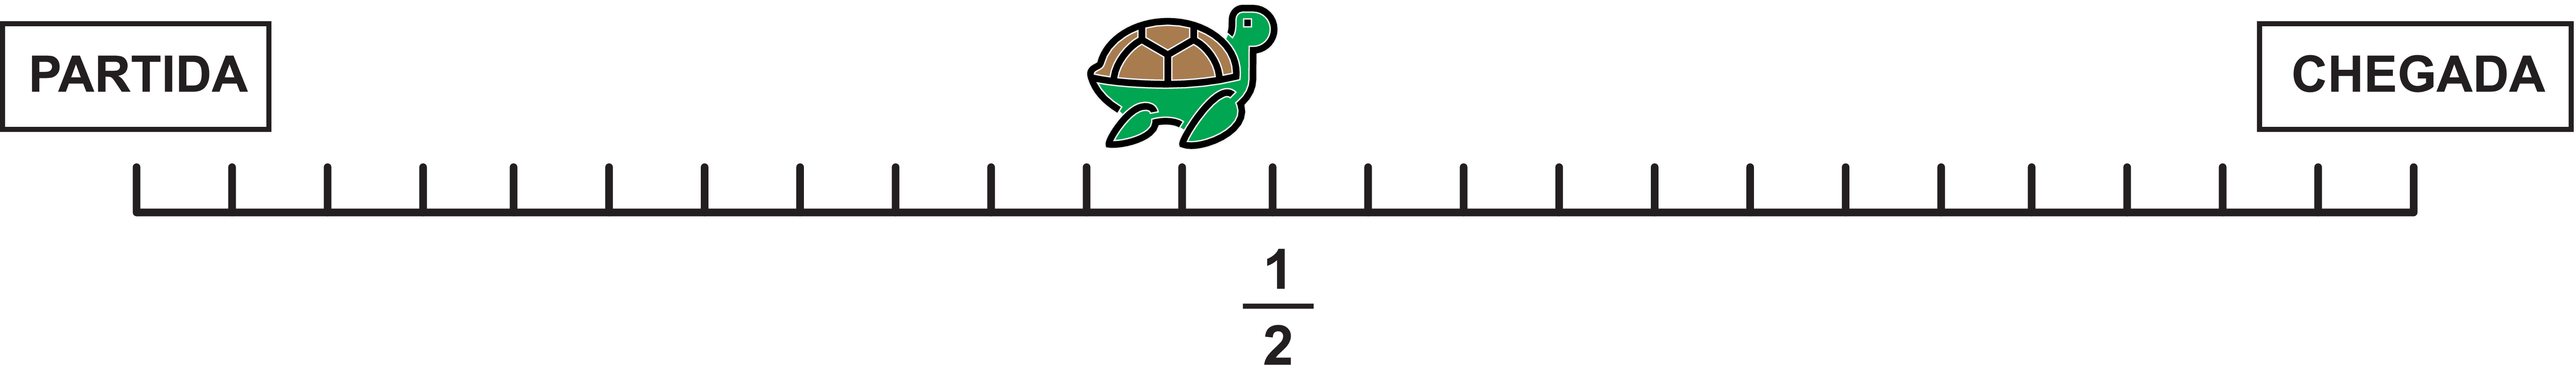
\includegraphics[width=195pt, keepaspectratio]{..//media/cap3/secoes/png/ativ9_resp_a}

\begin{enumerate} [\quad a)] %s
\item[b)]     Não está correta. Dividindo-se o percurso em quartos, como ilustra a figura a seguir, fica claro que o ponto correspondente a     $\frac{3}{4}$     do percurso está adiante da localização da tartaruga. Portanto, a tartaruga não percorreu mais do que     $\frac{3}{4}$     do percurso total.          

\end{enumerate}

 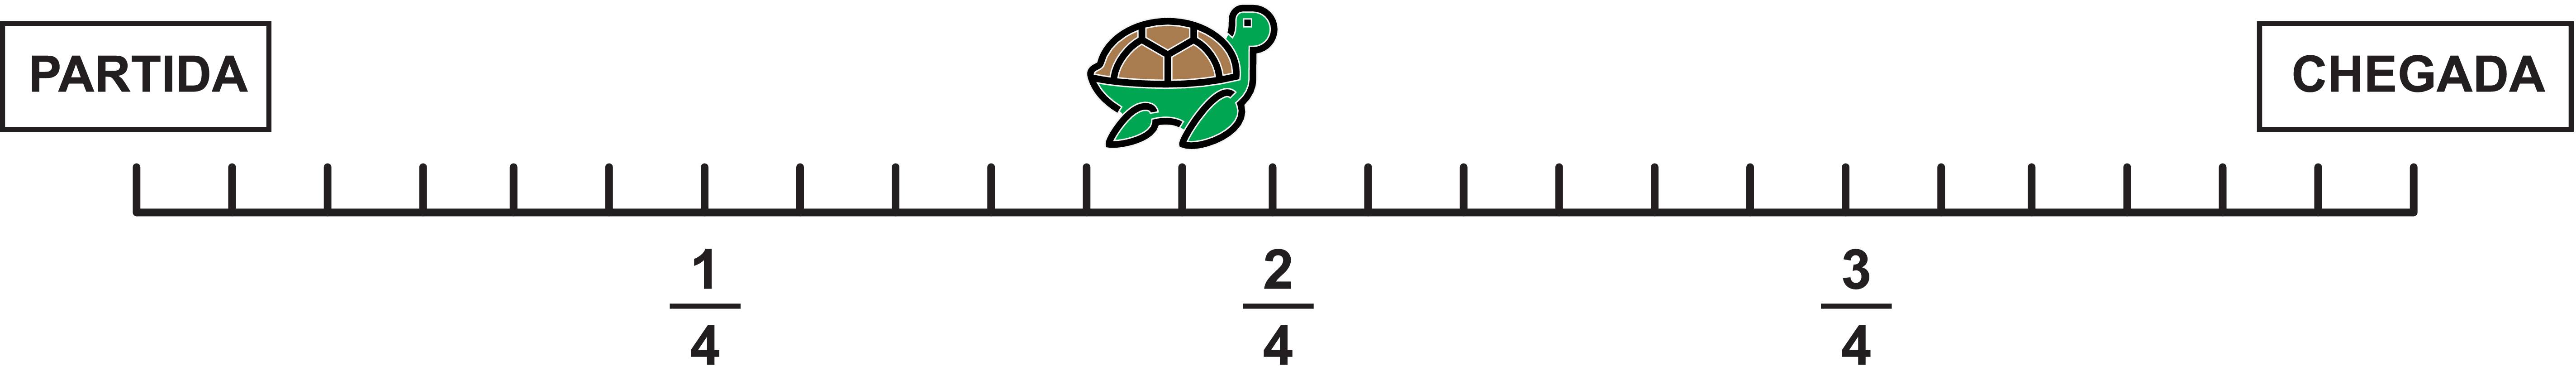
\includegraphics[width=195pt, keepaspectratio]{..//media/cap3/secoes/png/ativ9_resp_b}

\begin{enumerate} [\quad a)] %s


  \item[c)]     Está correta. Dividindo-se o percurso em oitavos, como ilustra a figura a seguir, fica claro que o ponto correspondente a     $\frac{3}{8}$     do percurso está antes da localização da tartaruga. Portanto, verifica-se que a tartaruga percorreu mais do que     $\frac{3}{8}$     do percurso total.          
\end{enumerate}

 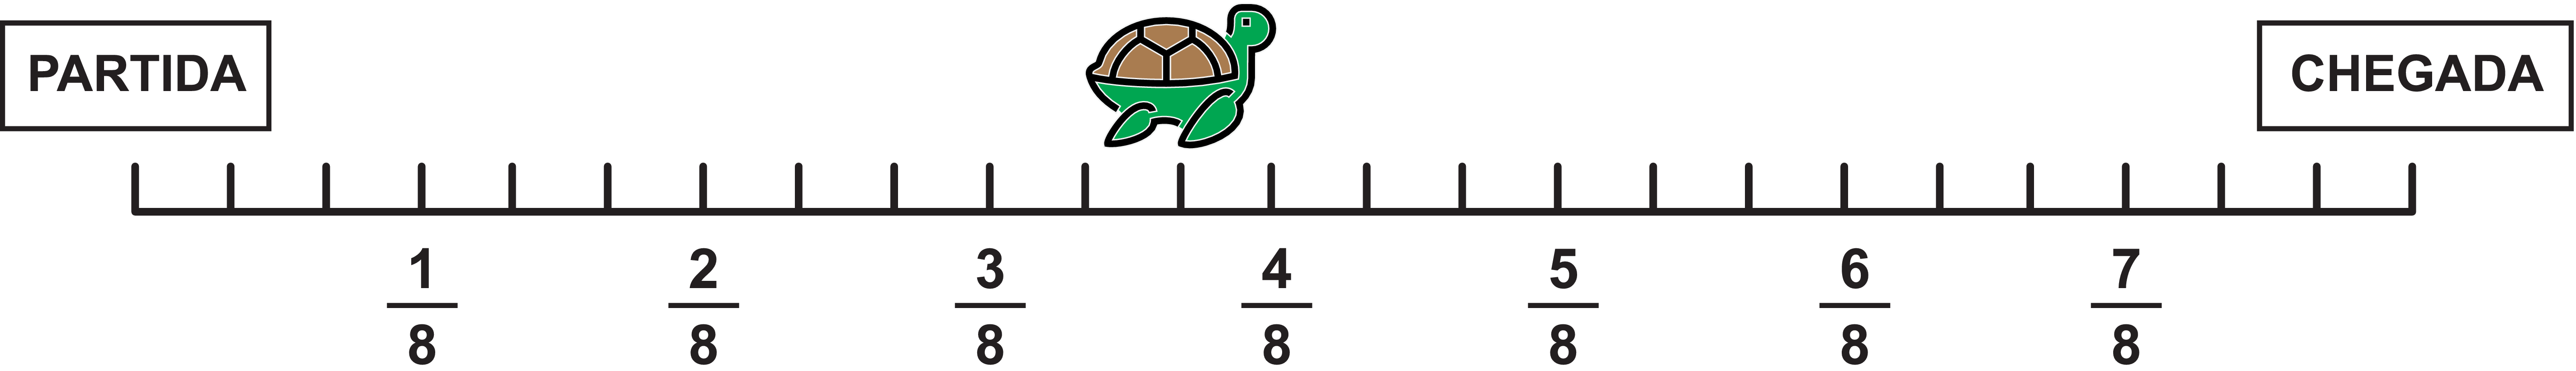
\includegraphics[width=195pt, keepaspectratio]{..//media/cap3/secoes/png/ativ9_resp_c}

\begin{enumerate} [\quad a)] %s
  \item[d)]     Está correta. Dividindo-se o percurso em quartos, como ilustra a figura a seguir, verifica-se que a localização da tartaruga é anterior ao ponto correspondente a     $\frac{3}{4}$     do percurso. Portanto, a tartaruga percorreu menos do que     $\frac{3}{4}$     do percurso total.         
\end{enumerate}

 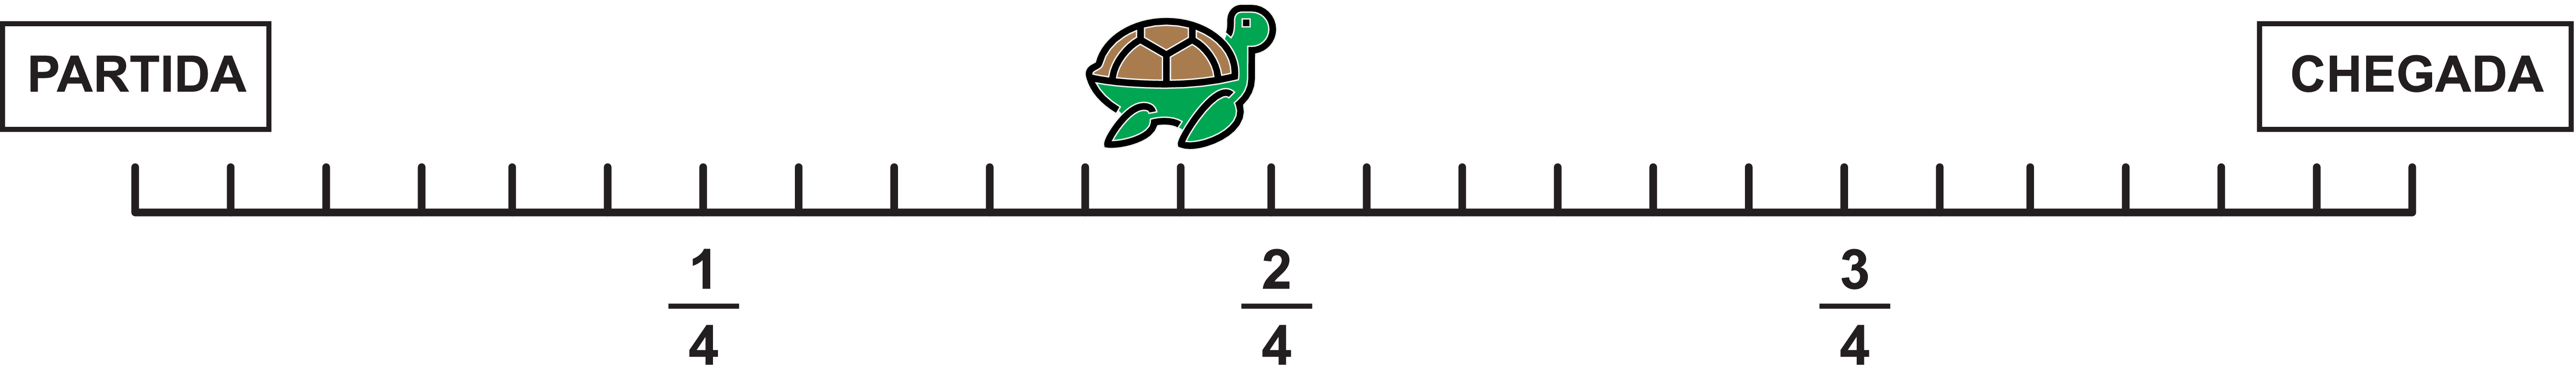
\includegraphics[width=195pt, keepaspectratio]{..//media/cap3/secoes/png/ativ9_resp_d}

\begin{enumerate} [\quad a)] %s
  \item[e)]     Não está correta. Dividindo-se o percurso em oitavos, como ilustra a figura a seguir, fica claro que o ponto correspondente a     $\frac{2}{8}$     do percurso está antes da localização da tartaruga. Portanto,verifica-se que tartaruga percorreu mais do que     $\frac{2}{8}$     do percurso.          
\end{enumerate}

 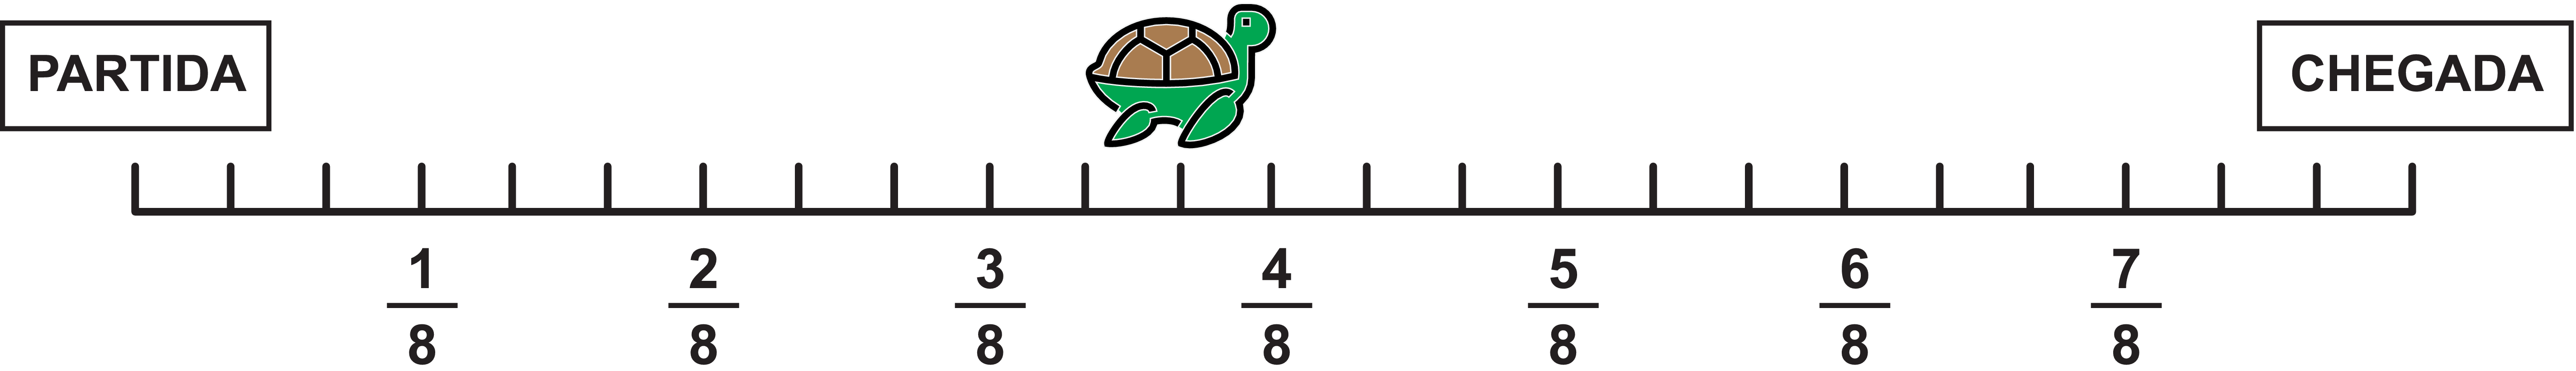
\includegraphics[width=195pt, keepaspectratio]{..//media/cap3/secoes/png/ativ9_resp_e}

\begin{enumerate} [\quad a)] %s

  \item[f)]     Está correta. Dividindo-se o percurso em terços, fica claro que o ponto correspondente a     $\frac{2}{3}$     do percurso está adiante da localização da tartaruga. Portanto, verifica-se que a tartaruga percorreu menos do que     $\frac{2}{3}$     do percurso          
\end{enumerate}

 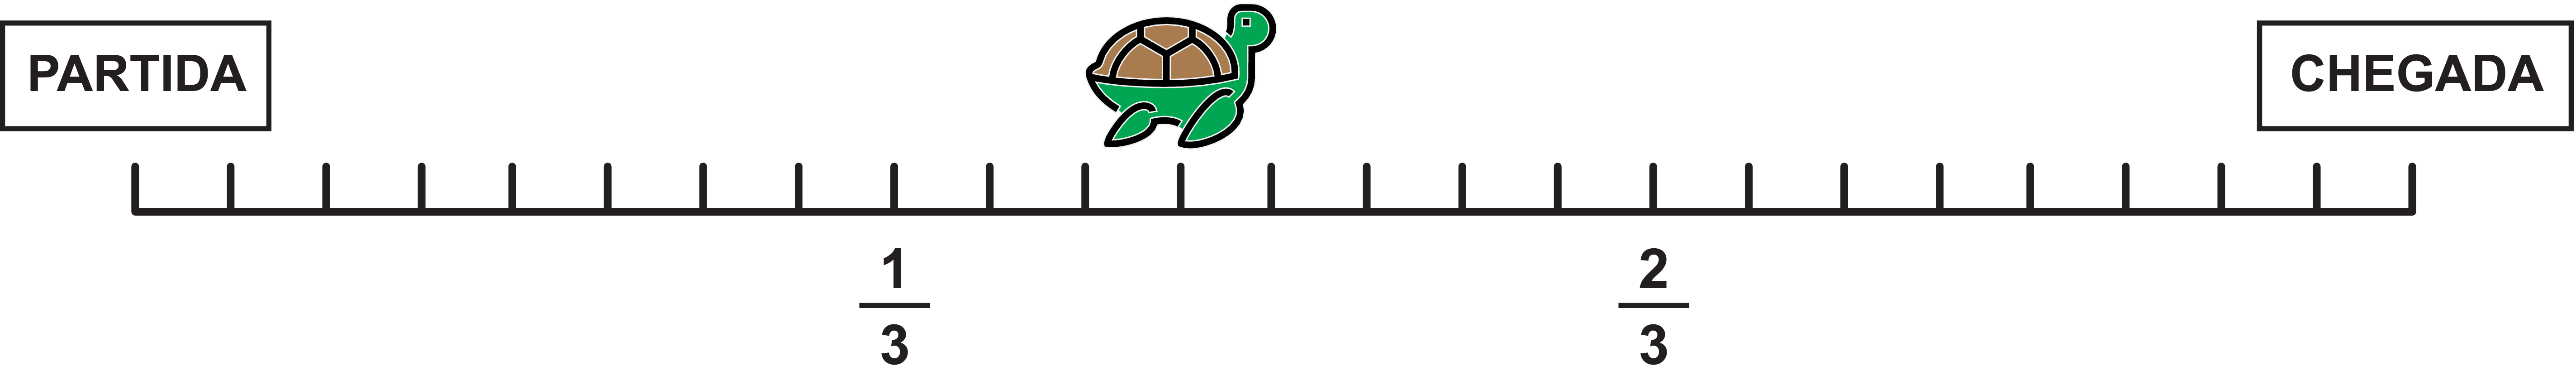
\includegraphics[width=195pt, keepaspectratio]{..//media/cap3/secoes/png/ativ9_resp_f}

\begin{enumerate} [\quad a)] %s

  \item[g)]     Não está correta. Dividindo-se o percurso em quartos, como ilustra a figura a seguir, fica claro que o ponto correspondente a     $\frac{3}{4}$     do percurso está adiante da localização da tartaruga. Portanto, verifica-se que a tartaruga percorreu menos do que     $\frac{3}{4}$     do percurso.          
\end{enumerate}

 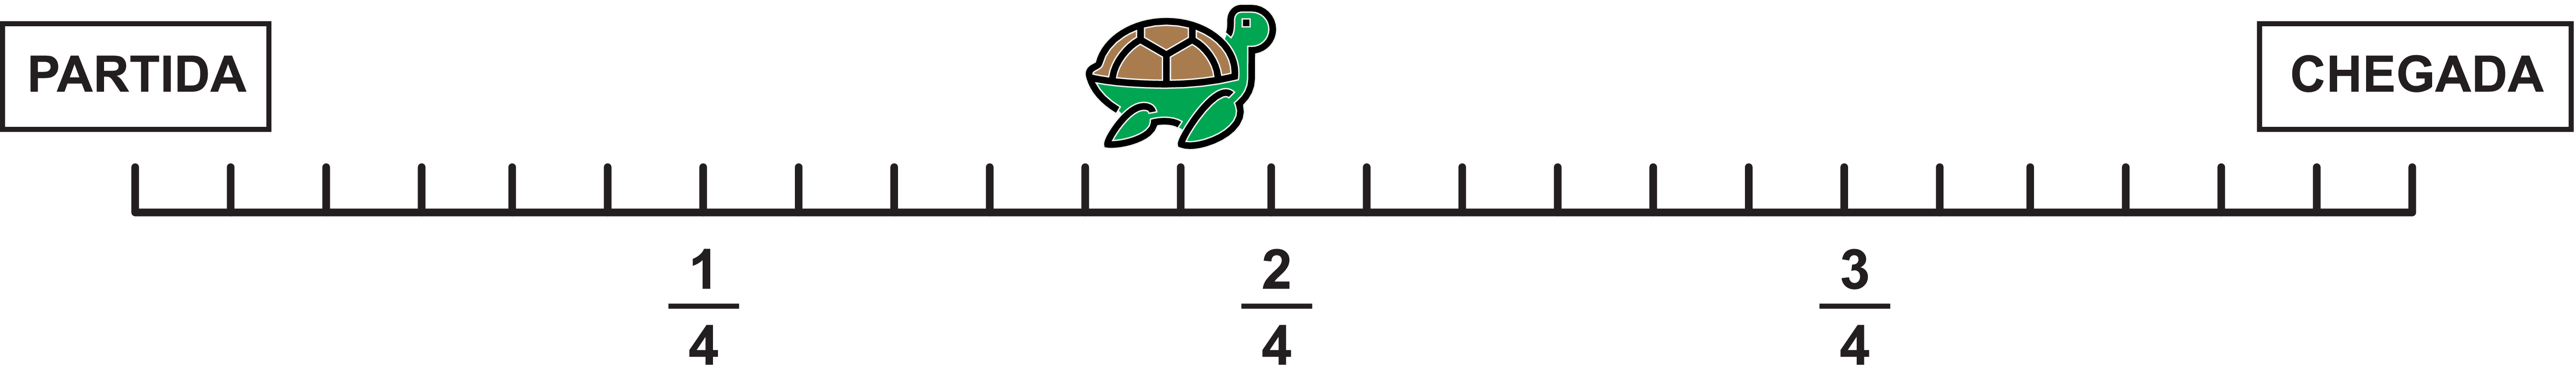
\includegraphics[width=195pt, keepaspectratio]{..//media/cap3/secoes/png/ativ9_resp_g}

\begin{enumerate} [\quad a)] %s

\item[h)]     Não está correta. Dividindo-se o percurso em oitavos, fica claro que o ponto correspondente a     $\frac{5}{8}$     do percurso está adiante da localização da tartaruga. Portanto,verifica-se que a tartaruga não alcançou     $\frac{5}{8}$     do percurso total.          
\end{enumerate}

 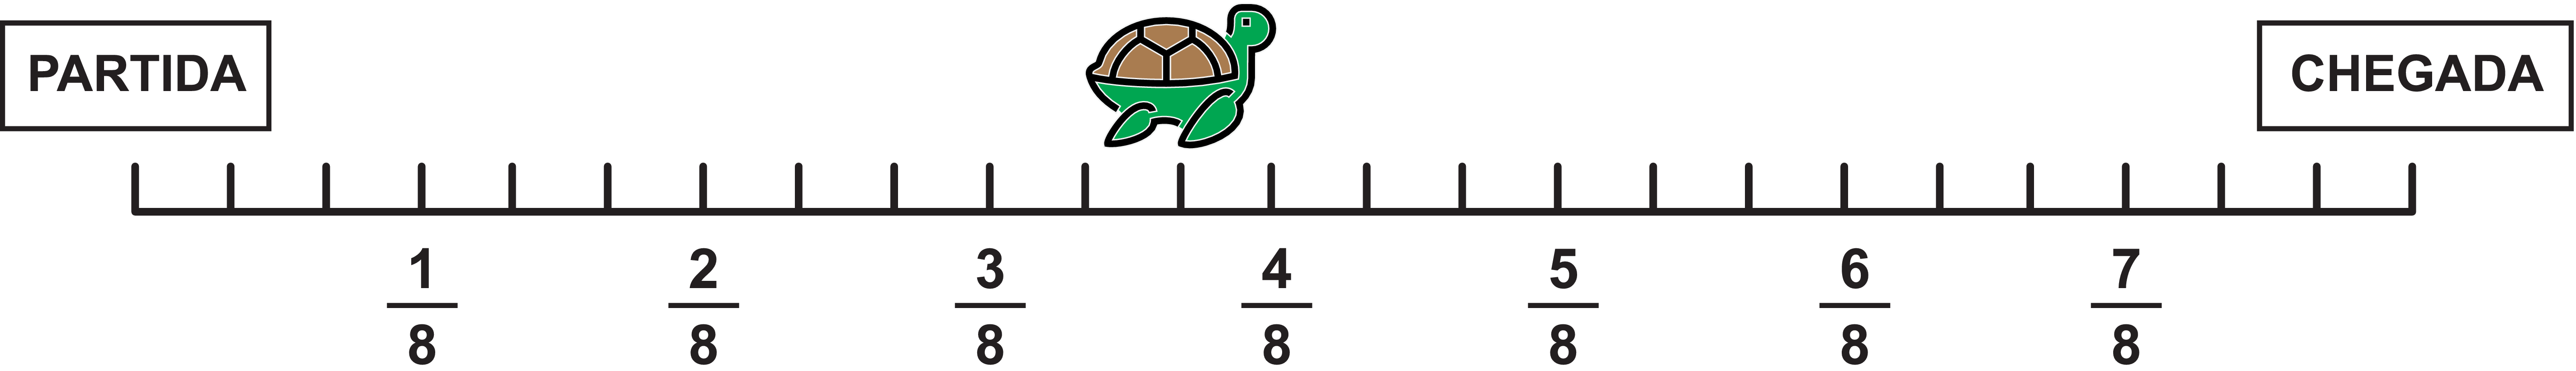
\includegraphics[width=195pt, keepaspectratio]{..//media/cap3/secoes/png/ativ9_resp_h}

\begin{enumerate} [\quad a)] %s

  \item[i)]     Está correta. De acordo com a resposta do item a), a tarataruga não alcançou a metade do percurso. Poranto, para alcançar a chegada, a tartaruga ainda precisa percorrer mais do que a metade do caminho.
  \item[j)]     Não está correta. A tartaruga já percorreu mais do que      $\frac{1}{3}$     do percurso e todo o percurso corresponde a      $\frac{3}{3}$    . Portanto, para alcançar a chegada, a tartaruga precisa percorrer menos do que     $\frac{2}{3}$     do caminho.
\end{enumerate} %s
\end{resposta*}

\subsection{Atividade 10}

\noindent {\bf Objetivos específicos: Levar o aluno a }  
\begin{itemize} %s
    \item       Representar frações na reta numérica, a partir da identificação da unidade;
    \item       Identificar, na reta numérica, os pontos correspondentes ao 0 e ao 1, a partir da represetação de duas frações (no caso, as frações       $\frac{1}{2}$       e       $\frac{3}{2}$      ).
    \item       Reconhecer a reta numérica em uma representação não comum.
\end{itemize} %s
      
\noindent {\bf Recomendações e sugestões para o desenvolvimento da atividade: }

\begin{itemize} %s
    \item       Recomenda-se que, nesta atividade, os alunos trabalhem individualmente. No entanto, é fundamental que os alunos sejam estimulados a explicar o raciocínio realizado.
    \item       Observe que a reta numérica não é apresentada da forma mais tradicional, paralela a uma das margens da página e na direção comumente chamada de horizontal. O objetivo é ampliar e variar o contato com esse modelo de representação. 
    \item       Além disso, os pontos que identificam frações da unidade (no caso, décimos) também são determinados de uma forma não tradicional. A divisão é estabelecida a partir de um feixe de retas paralelas igualmente espaçadas  e transversal a reta numérica em destaque. 
    \item       Os dois primeiros itens desta atividade são bastante simples, apesar da representação não tradicional. 
    \item       O terceiro item desta atividade objetiva que o aluno identifique os pontos correspondentes ao 0 e ao 1, que determinam o segmento unitário na reta numérica, a partir dos pontos correspondentes às frações       $\frac{1}{2}$       e       $\frac{3}{2}$.  
\end{itemize} %s

\begin{resposta*}{Atividade 10}


a)

\begin{tikzpicture}[x=56.25mm,y=56.25mm, scale=.9]
 
\begin{scope}
\clip (-.2,-.2) rectangle (.85,.85); 
 
\begin{scope}[ rotate=45]
\foreach \x in {-1.1,-1,...,1.6}{
\draw[common] (\x,0) --+ (45:1); 
\draw[common] (\x,0) --+ (45:-1);}
 
\draw[attention] (-0.2,0) -- (1.2,0) ; %edit here for the axis
\foreach \x in {0,1}{ \draw (\x,3pt) -- (\x,-3pt) node[below] {\x};}
\foreach \x in {0.1,.2,...,.9}{ \draw (\x,3pt) -- (\x,-3pt);}
 
\fill[common] (.5,0) circle (3pt) node[below, black] {$\frac{1}{2}$};
 
\end{scope}
\end{scope}
 
\end{tikzpicture}   
\vspace{.5cm}
 

b)

\begin{tikzpicture}[x=56.25mm,y=56.25mm, scale=.9]
 
\begin{scope}
\clip (-.2,-.2) rectangle (.85,.85); 
 
\begin{scope}[ rotate=45]
\foreach \x in {-1.1,-1,...,1.6}{
\draw[common] (\x,0) --+ (45:1); 
\draw[common] (\x,0) --+ (45:-1);}
 
\draw[attention] (-0.2,0) -- (1.2,0) ; %edit here for the axis
\foreach \x in {0,1}{ \draw (\x,3pt) -- (\x,-3pt) node[below] {\x};}
\foreach \x in {0.1,.2,...,.9}{ \draw (\x,3pt) -- (\x,-3pt);}
 
\foreach \x in {1,2,...,9} \node[below] at (\x/10,0) {$\frac{\x}{10}$};
\fill[common] (.5,0) circle (3pt) node[above, black] {$\frac{1}{2}$};
\end{scope}
\end{scope}
 
\end{tikzpicture}   
\vspace{.5cm}
 
c)

\begin{tikzpicture}[x=56.25mm,y=56.25mm, scale=.9]
 
\begin{scope}
\clip (-.2,-.2) rectangle (.85,.85); 
 
\begin{scope}[ rotate=45]
\foreach \x in {-1.1,-1,...,1.6}{
\draw[common] (\x,0) --+ (135:1); 
\draw[common] (\x,0) --+ (135:-1);}
 
\draw[blue] (-0.2,0) -- (1.2,0) ; %edit here for the axis
\foreach \x in {0,0.1,.2,...,.9}{ \draw (\x,3pt) -- (\x,-3pt);}
\fill[common] (.2,0) circle (3pt) node[below, black] {$\frac{1}{2}$};
\fill[common] (.6,0) circle (3pt) node[below, black] {$\frac{3}{2}$};
\fill[attention] (0,0) circle (3pt) node[below, black] {0};
\fill[attention] (.4,0) circle (3pt) node[below, black] {1};
\end{scope}
\end{scope}
 
\end{tikzpicture}   
\vspace{.5cm}
 
d)
 
\begin{tikzpicture}[x=56.25mm,y=56.25mm, scale=.9]
 
\begin{scope}
\clip (-.2,-.2) rectangle (.85,.85); 
 
\begin{scope}[ rotate=45]
\foreach \x in {-1.1,-1,...,1.6}{
\draw[common] (\x,0) --+ (135:1); 
\draw[common] (\x,0) --+ (135:-1);}
 
\draw[blue] (-0.2,0) -- (1.2,0) ; %edit here for the axis
\foreach \x in {0,0.1,.2,...,.9}{ \draw (\x,3pt) -- (\x,-3pt);}
\fill[common] (.2,0) circle (3pt) node[below, black] {$\frac{1}{2}$};
\fill[common] (.6,0) circle (3pt) node[below, black] {$\frac{3}{2}$};
\fill[attention] (.3,0) circle (3pt) node[below, black] {$\frac{3}{4}$};
\fill[attention] (.5,0) circle (3pt) node[below, black] {$\frac{5}{4}$};
\end{scope}
\end{scope}
 
\end{tikzpicture}

\end{resposta*}

% \end{multicols}
\subsection{Sobre o Organizando as Ideias}



Após o Organizando as Idéias, passar-se-á a falar apenas em ``fração'' ao referir-se a frações na reta numérica, subentendendo que já esteja claro aos alunos que trata-se de uma ``fração da unidade'', unidade que já está identificada na reta pelo segmento de extremos 0 e 1, mesmo que estes estejam implícitos a partir de alguma outra informação.

Espera-se que, ao longo desta lição, o aluno tenha associado fração a uma quantidade. Assim, no parágrafo que trata sobre a ordem na reta numérica, fala-se nos ``números representados na reta numérica'', incluindo-se, entre eles, as frações.

Lembre que a justaposição de segmentos pode sempre ser feita com a ajuda do compasso, evitando-se assim, medida.

\Bg
\Bg


% \begin{multicols}{2}
\subsection{Atividade 11}

\noindent {\bf Objetivos específicos: Levar o aluno a}
\begin{itemize} %s
  \item     Reconhecer a representação das frações na reta numérica;
  \item     Ordenar frações. 
\end{itemize} %s

\noindent {\bf Material necessário:}
\begin{itemize} %s
  \item     Pelo menos     $3$     metros de barbante, de maneira que cubra toda uma lateral da sala de aula (por exemplo, aquela em que está posicionado o quadro. 
  \item         $4$     folhas de papel sufite. 
  \item         $32$     pregadores de roupa (podem ser substituídos por clipes de papel).
  \item     Fita adesiva.
\end{itemize} %s

\noindent {\bf Preparação para a atividade:}
\begin{itemize} %s
  \item     Esta atividade deve ser desenvolvida como um jogo, envolvendo todos os alunos da turma, organizados em grupos  5 ou 6 alunos. A quantidade de participantes em cada grupo e, consequentemente, a quantidade de grupos, deve ser decidida tendo em conta a quantidade de alunos na turma. Tudo deve ser combinado e esclarecido antes de a atividade começar.
  \item     O professor deve fazer um  ``varal'' com o barbante em um local que seja visível para todos os alunos e não muito alto para que os estudantes possam alcançar com as mãos. Pode ser, por exemplo, em frente ao quadro, e indo de um extremo a outro da sala. Esse barbante representará a reta numérica. 
  \item O objetivo da atividade é ``pendurar os números'' no barbante usando pregadores ou fitas adesivas, visando experimentar, em uma atividade concreta, a associação entre os pontos da reta e os números. Para isso serão feitos cartões numerados. 
  \item É Importante reforçar a fixacão das extremidades do barbante para que não solte com o peso dos cartões que serão pendurados.
  \item Dobre cada uma das folhas de papel $2$ vezes ao meio, em direções paralelas aos lados, marcando assim 4 retângulos congruentes em cada folha. Recorte esses retângulos. Cada um deles será numerado e, durante a atividade, fixado no barbante. Serão chamados de {\bf cartões numerados} (como os da figura). 
  \item  Escreva as os números $0$, $1$, $2$, $3$, $\frac{1}{2}$, $\frac{2}{2}$, $\frac{3}{2}$, $\frac{4}{2}$, $\frac{5}{2}$, $\frac{6}{2}$, $\frac{1}{3}$, $\frac{2}{3}$, $\frac{3}{3}$, $\frac{4}{3}$, $\frac{7}{3}$, $\frac{9}{3}$, $\frac{1}{4}$, $\frac{2}{4}$, $\frac{3}{4}$, $\frac{4}{4}$, $\frac{5}{4}$, $\frac{6}{4}$, $\frac{8}{4}$, $\frac{10}{4}$, $\frac{11}{4}$, $\frac{12}{4}$, $\frac{1}{5}$, $\frac{3}{5}$, $\frac{4}{5}$, $\frac{6}{5}$, $\frac{7}{5}$, $\frac{10}{5}$, $\frac{1}{10}$ nesses cartões.
  \item Observe que são contemplados números naturais e frações não inteiras. 
  \item Além dos cartões numerados com o $0$ (zero) e o $1$ (um) , recomenda-se que haja pelo menos um cartão numerado para cada aluno. A sequência com $32$ números é uma sugestão básica. Essa sequência pode ser ampliada (ou reduzida) a partir da avaliação do professor. 
\end{itemize} %s

\noindent {\bf Recomendações e sugestões para o desenvolvimento da atividade:}
\begin{itemize}
  \item O desenvolvimento da atividade precisa ser mediado pelo professor. O processo e a discussão são importantes.
  \item As fichas com o $0$ (zero) e com o $1$ (um) devem ser presas no barbante pelo professor com fita adesiva antes do início da atividade, porque a distância entre o $0$ (zero) e o $1$ (um) terá o papel de unidade para o estudante determinar a posição dos demais cartões. {\bf Isso deve ser feito a vista dos alunos para ressaltar que a unidade é escolhida}. 
  \item Caso seja utilizado um barbante de $3$ metros, o zero pode ser posicionado bem próximo à extremidade e o número um a 90 cm à direita do zero.
  \item Combine tas regras com os alunos.
  \item Recomenda-se que os grupos sejam identificados, por exemplo, por cores para facilitar a comunicação. Cada grupo, na sua vez de jogar, deve fixar um cartão numerado no varal e outro grupo deve avaliar se o cartão foi fixado em uma posição correta ou não.
  \item Distribua os cartões igualmente entre os grupos formados. 
  \item A correção da fixação realizada por um grupo deve ser decidida por outro grupo, podendo ser discutida com toda a turma. 
  \item Pontuacão: cada cartão numérico posicionado corretamente vale um ponto para o grupo que fixou o cartão. Cada avaliação correta vale meio ponto para o grupo que ficou responsável por ela. 
  \item Vence o jogo o grupo que, após a fixação de todos os cartões numerados no varal, tiver acumulado maior quantidade de pontos. 
  \item Em cada rodada, todos os grupos devem prender um cartão numérico no varal e avaliar a colcação feita por outro grupo. Varie as duplas de grupos que farão as ações de fixação/avaliação de cada cartão preso no varal. Assim, por exemplo, se a turma estiver organizada em $5$ grupos (Azul, Verde, Vermelho, Amarelo e Preto), com 6 alunos cada um, na prmeira rodada as duplas que farão a fixação/avaliação podem ser, por exemplo, azul/preto, verde/vermelho, vermelho/azul, amarelo/verde e preto/amarelo. Já na segunda rodada as duplas podem ser azul/amarelo, verde/preto, vermelho/verde, amarelo/azul e preto/vermelho. Planeje previamente essas associações e comunique aos alunos para não gerar discussão durante a realização 
  \item Incentive e procure fazer, respeitando as questões pessoais, com que todos os alunos façam a fixação de pelo menos um cartão numerado no varal. 
  \item Escolha o grupo com o número $2$ para dar início ao jogo. Em seguida aquele que tiver o número 3. Claro que esses números serão mais facilmente posicionados no varal. Essa decisão pode ser uma estratégia deles no jogo. Além disso, quando já presos no varal, facilitarão a fixação dos demais. Pode acontecer de esses grupos não escolherem inicialmente esses catões. No entanto, quando esses cartões forem os escolhidos pelos respectivos grupos para serem fixados no barbante, discusta a relevância dessas referências para facilitar a fixação dos demais números, não inteiros.      
  \item Observe que alguns cartões numerados ocuparão a mesma posição na reta. Por exemplo, os numerados com $2$ e $\frac{4}{2}$. Nesses casos, recomenda-se que o segundo cartão a ser fixado seja preso no que já está no varal, sem que um esconda o outro. Sugere-se um abaixo do outro. Aproveite esses casos para discutir com os alunos que um mesmo número pode ter mais do que uma representação.
  \item Muito provavelmente as frações de denominador $2$ serão as mais fáceis de serem fixadas no varal. Em seguida, as de denominador $4$. As fixação das frações de denominadores $3$, $5$ e $10$ devem impor um pouco mais de desafio. Garanta que haja euilíbrio de dificuldade na distribuição dos cartões numerados entre os grupos.
  \item Estimule a discussão interna nos grupos para a decisão da posição de fixação de cada cartão numerado. O aluno eleitopelo grupo para prende o cartão no barbante deve explicar como decidiram por aquela posição.
  \item A atividade pode ser refeita recolhendo-se os cartões das frações do varal, colocando-os embaralhados sobre a mesa do professor com as faces voltadas para baixo e cada estudante deve ir à mesa do professor pegar um cartão e prendê-lo no varal.
  \item Uma variação desse jogo pode admitir que um grupo sugira frações para que outro grupo faça a fixação. Nesse caso, as frações podem ser escolhidas a partir de uma lista previamente estabelecida pelo professor. Nesse caso, recomneda-se que o grupo que escolhe a fração deverá lê-la e o grupo que fará a fixação deverá registá-la. Dessa forma, a leitura e a escrita em representação simbólica também são tratadas na atividade.
\end{itemize} %s

\begin{resposta*}{Atividade 11}

Para facilitar a visualização apresentamos a solução em duas retas.
\begin{center}
\begin{tikzpicture}[x=18mm,y=34mm]
\draw[->] (-0.1,0) -- (4,0) ; %reta anterior
\foreach \x in {0,.1,...,3.9}{ \draw (\x,1pt) -- (\x,-1pt);}
\foreach \x in {0,1,2,3} \node at (\x,-30pt) {\x}; 
\foreach \x in {1,2,3,4,5,6} {\draw[fill=attention] (\x/2, 0) circle (1pt); \node[above] at (\x/2,3pt) {$\frac{\x}{2}$};}
\foreach \x in {1,2,3,4,7,9} {\draw[fill=common] (\x/3, 0) circle (1pt); \node[below] at (\x/3,0) {$\frac{\x}{3}$};}
\end{tikzpicture}

\begin{tikzpicture}[x=18mm,y=34mm]
\draw[->] (-0.1,0) -- (4,0) ; %reta anterior
\foreach \x in {0,.1,...,3.9}{ \draw (\x,1pt) -- (\x,-1pt);}
\foreach \x in {1,2,3,4,5,6,8,10,11,12} {\draw[fill=attention] (\x/4, 0) circle (1pt); \node[above] at (\x/4,3pt) {$\frac{\x}{4}$};}
\foreach \x in {1,3,4,6,7,10} {\draw[fill=common] (\x/5, 0) circle (1pt); \node[below] at (\x/5,0) {$\frac{\x}{5}$};}
\node[above] at (.1,3pt) {$\frac{1}{10}$};
\end{tikzpicture}

\end{center}

\end{resposta*}


\subsection{Atividade 12}
  
  \noindent {\bf Objetivo específico:}   
\begin{itemize} %s
    \item       Representar frações na reta numérica.
    \item       Comparar frações.
\end{itemize} %s
  
  \noindent {\bf Recomendações e sugestões para o desenvolvimento da atividade: }
\begin{itemize}  
     \item  Recomenda-se que esta atividade seja realizada individualmente. No entanto, a discussão das resposta deve ser feita com toda a turma. Estimule seus alunos a explicarem suas respostas.  
     \item  A associação das frações aos pontos correspondentes exigirá estratégias e comparações variadas. Procure identificar e discutir as argumentações apresentadas pelos alunos.   
     \item  Todos os pontos necessários para estabelecer as associações solicitadas estão evidenciados na figura, no entanto, nem todos são imediatos.  
     \item  Inicialmente os alunos precisam identificar que as marcações em destaque identificam oitavos. Assim, por exemplo, para identificar quartos, precisará reunir dois oitavos e para marcar   $\frac{3}{2}$   precisará contar 12 oitavos.  
     \item  Esta atividade oferece também, de forma indireta, a oportunidade de os alunos estabelecerem comparações. Por exemplo, reconhecer que   $\frac{3}{4}$   é menor do que 1 e que   $\frac{5}{4}$   é maior, que   $\frac{8}{4}$   = 2 e que   $\frac{10}{4}$   é menor do que   $\frac{10}{8}$  . Destaque e discuta essas e outras comparações com os seus alunos.   
\end{itemize}      
 
\begin{resposta*}{Atividade 12}
\noindent
\begin{tikzpicture}[xscale=.27]
	
	\draw[->]  (-.5,0) -- (26,0);
	\draw  (0,-3pt) -- (0,3pt);
	\draw  (1.25,-3pt) -- (1.25,3pt);
	\draw  (2.5,-3pt) -- (2.5,3pt);
	\draw  (3.75,-3pt) -- (3.75,3pt);
	\draw  (5,-3pt) -- (5,3pt);
	\draw  (6.25,-3pt) -- (6.25,3pt);
	\draw  (7.5,-3pt) -- (7.5,3pt);
	\draw  (8.75,-3pt) -- (8.75,3pt);
	\draw  (10,-3pt) -- (10,3pt);
	\draw  (11.25,-3pt) -- (11.25,3pt);
	\draw  (12.5,-3pt) -- (12.5,3pt);
	\draw  (13.75,-3pt) -- (13.75,3pt);
	\draw  (15,-3pt) -- (15,3pt);
	\draw  (16.25,-3pt) -- (16.25,3pt);
	\draw  (17.5,-3pt) -- (17.5,3pt);
	\draw  (18.75,-3pt) -- (18.75,3pt);
	\draw  (20,-3pt) -- (20,3pt);
	\draw  (21.25,-3pt) -- (21.25,3pt);
	\draw  (22.5,-3pt) -- (22.5,3pt);
	\draw  (23.75,-3pt) -- (23.75,3pt);
	\draw  (25,-3pt) -- (25,3pt);

	\node[above] at (0,3pt)  {0};

	\node[below] at (5,0) {$\frac{1}{2}$};

	\node[above] at (10,3pt)  {1};

	\node[below] at (15,0) {$\frac{3}{2}$};
	
	\node[below] at (7.5,0) {$\frac{3}{4}$};

	\node[below] at (12.5,0) {$\frac{5}{4}$};
	
	\node[below] at (20,0) {$\frac{8}{4}$};

	\node[above] at (20,3pt) {2};
	
	\node[below] at (25,0) {$\frac{10}{4}$};

	\node[below] at (1.25,0) {$\frac{1}{8}$};

	\node[below] at (8.75,0) {$\frac{7}{8}$};

	\node[above] at (12.5,3pt) {$\frac{8}{10}$};
\end{tikzpicture}


\end{resposta*}


\subsection{Atividade 13}


\noindent {\bf Objetivo específico: :}
  \begin{itemize}
   \item Representação de frações $\frac{1}{d}$ na reta numérica.
   \item Comparação de frações $\frac{1}{d}$ na reta numérica.
  \end{itemize}
 

\noindent {\bf Recomendações e sugestões para o desenvolvimento da atividade:}
   \begin{itemize} 
    \item Recomenda-se que esta atividade seja realizada individualmente. No entanto, a discussão das resposta deve ser feita com toda a turma. Estimule seus alunos a explicarem suas respostas.
   \item  Observe e discuta com seus alunos que, no caso das frações de numerador igual a $1$ (frações $\frac{1}{d}$), quanto maior o denominador, menor a fração. Portanto, sua representação na reta numérica está mais perto do zero. 
   \item  Aproveite para propor e discutir com seus alunos algumas reflexões tais como: 
   \begin{enumerate}[(i)]
    \item Alguma com numerador igual pode ter sua representação na reta numérica entre $\frac{1}{2}$ e 1?
    \item Qual fração é maior, $\frac{1}{4}$ ou $\frac{1}{10}$?  
    \item Que fração tem sua representação na reta numérica mais próxima de 0, $\frac{1}{5}$ ou $\frac{1}{6}$?
   \end{enumerate}
 
  \end{itemize}
  

\begin{resposta*}{Atividade 13}

As respostas são na ordem I, A, B, H, F, C, E, D e G. 

\end{resposta*}

\subsection{Atividade 14}

\noindent {\bf Objetivo específico:}  Comparação de frações unitárias em sua representação simbólica.

\noindent {\bf Recomendações e sugestões para o desenvolvimento da atividade:}
\begin{itemize}
 \item  Recomenda-se que esta atividade seja realizada individualmente. No entanto, a discussão das resposta deve ser feita com toda a turma. Estimule seus alunos a explicarem suas respostas.
 \item  Esta atividade é complementar da anterior. Na atividade anterior, as frações estão representadas na reta numérica. Nesta, as frações unitárias são apresentadas em sua representaçã simbólica, na forma $\frac{a}{b}$. Espera-se que os alunos consigam compará-las fazendo relação com a representação na reta numérica, tratada na atividade anterior. Assim, por exemplo, a desigualdade $\frac{1}{10} < \frac{1}{4}$ pode ser justificada pelo fato de que, na representação na reta numérica, a fração $\frac{1}{10}$ está mais próxima do ponto correspondente ao zero do que a fração $\frac{1}{4}$. 
\end{itemize}

\begin{resposta*}{Atividade 14}
\begin{enumerate}[a)]
 \item $\frac{1}{2}>\frac{1}{5}$.
\item $\frac{1}{4}<\frac{1}{3}$.  
\item $\frac{1}{10}>\frac{1}{20}$. 
\item $\frac{1}{12}<\frac{1}{2}$.
\item $\frac{1}{35}>\frac{1}{43}$.
\item  $\frac{1}{99}>\frac{1}{100}$.
\item  $\frac{1}{5}>\frac{1}{50}$.
\item  $\frac{1}{100}<\frac{1}{10}$.
\end{enumerate}
 
\end{resposta*}


\subsection{Atividade 15}
  
  \noindent {\bf Objetivo específico:   }
\begin{itemize} %s
    \item       Comparação de frações com o mesmo numerador ou com o mesmo denominador, a partir de um referencial.
\end{itemize} %s
  
  
\noindent {\bf Recomendações e sugestões para o desenvolvimento da atividade: }
\begin{itemize}
    \item       Recomenda-se que esta atividade seja realizada em duplas. No entanto, a discussão das resposta deve ser feita com toda a turma.
    \item       Estimule seus alunos a explicarem suas respostas.
    \item       A associação das frações aos pontos correspondentes exigirá que os alunos saibam associar pontos na reta numérica às frações correspondentes e que façam comparações de diferentes tipos. Valorize e discuta as diversas estratégias apresentadas pelos alunos. 
    \item       Por exemplo, uma vez que os pontos correspondentes a 0, a 1 e a       $\frac{1}{2}$       já estão destacados, é natural que as primeiras frações a serem associadas a pontos na reta numérica sejam       $\frac{1}{4}$       e       $\frac{3}{4}$. Em seguida, reconhecendo que       $\frac{1}{8}$       corresponde à metade de       $\frac{1}{4}$,  as frações       $\frac{3}{8}$       e       $\frac{5}{8}$       podem ser as próximas.  Na sequência, o aluno pode reconhecer que       $\frac{4}{5}$       e       $\frac{9}{10}$       são menores do que a unidade e que       $\frac{9}{8}$       e       $\frac{11}{10}$       são maiores.  Entre       $\frac{4}{5}$       e       $\frac{9}{10}$,       $\frac{9}{10}$       pode ser identificada como maior por faltar  apenas       $\frac{1}{10}$       para compor a unidade , enquanto que para       $\frac{4}{5}$       falta       $\frac{1}{5}$       da unidade. Por fim, por raciocínio análogo, a fração       $\frac{9}{8}$       pode ser identificada como maior do que       $\frac{11}{10}$, por ser       $\frac{1}{8}$       maior do que a unidade, enquanto que       $\frac{11}{10}$       é apenas       $\frac{1}{10}$       maior. 
    \item       Se achar necessário, discuta a comparação entre alguns pares das frações apresentadas antes de os alunos resolverem a atividade. Por exemplo, peça-os que comparem       $\frac{3}{8}$        e       $\frac{5}{8}$, que são frações com o mesmo denominador. Ou que comparem       $\frac{9}{8}$       e       $\frac{9}{10}$, que envolvem frações com o mesmo numerador.
    \item       O aluno pode responder simplesmente       ``ligando''       os cartões com as frações aos pontos correspondentes na reta numérica. No entanto, recomenda-se que o professor solicite que escrevam as frações abaixo dos pontos corrrespentes na reta numérica, a exemplo do 0, do 1, e de       $\frac{1}{2}$.
\end{itemize} %s
 
\begin{resposta*}{Atividade 15}

\begin{tikzpicture}
\begin{scope}[scale=.15]
	\draw  (-2,0) -- (45,0);
	\draw[->]  (45,0) -- (47,0);

	
	\node  at (0,-1) {0};						%0
	\node  at (20,-1.75) {$\frac{1}{2}$};		%1/2
	\node  at (40,-1) {1};					%1

	\node  at (10,-1.75) {$\frac{1}{4}$};			%1/4
	\node  at (15,-1.75) {$\frac{3}{8}$};			%3/8

	\node  at (25,-1.75) {$\frac{5}{8}$};			%5/8
	\node  at (30,-1.75) {$\frac{3}{4}$};			%3/4
	\node  at (32,-1.75) {$\frac{4}{5}$};			%4/5
	\node  at (36,-1.75) {$\frac{9}{10}$};			%9/10

	\node  at (43.5,-1.75) {$\frac{11}{10}$};		%11/10
	\node  at (45.5,-1.75) {$\frac{9}{8}$};			%9/8
\end{scope}
	
	\foreach \x in {0,10,15,20,25,30,32,36,40,44,45} \fill[common] (\x*.15,0) circle (2pt);

\end{tikzpicture}
  
\end{resposta*}

\subsection{Atividade 16}

\noindent {\bf Objetivo específico:}   Comparação de frações.

\noindent {\bf Recomendações e sugestões para o desenvolvimento da atividade:}
   \begin{itemize}
   \item   Recomenda-se que esta atividade seja realizada individualmente. No entanto, a discussão das resposta deve ser feita com toda a turma. Estimule seus alunos a explicarem suas respostas.
   \item Nesta atividade, as frações são apresentadas apenas em sua representação simbólica na forma $\frac{a}{b}$. Espera-se que os alunos consigam compará-las a partir da ideia de quantidade, sem necessariamente recorrer às representações em modelos contínuos ou na reta numérica. Assim, por exemplo, a comparação entre $\frac{1}{2}$ e $\frac{1}{3}$ fica estabelecida pelo fato de que a primeira identifica uma das partes da equipartição da unidade por dois, enquanto que $\frac{1}{3}$ identifica uma das partes da equipartição da mesma unidade por três. Logo, $\frac{1}{2} > \frac{1}{3}$. 
   \item No entanto, é importante observar que alguns alunos podem precisar do apoio das demais representações citadas. A discussão de cada item deve ser amparada por pelo menos as três estratégias destacadas: (i) argumentação verbal amparada pela ideia de quantidade; (ii) representação em modelos contínuos e (iii) representação na reta numérica. Por exemplo, na correção do item a), entre $\frac{3}{6}$ e $\frac{5}{6}$, espera-se que a discussão contemple:
   \begin{enumerate}[(i)]
    \item o fato de que, como essas frações indicam quantidades de ``sextos'', a menor (maior) é aquela que têm menor (maior) numerador. Portanto, $\frac{3}{6}< \frac{5}{6}$. 
    \item A representação em modelos contínuos: 
   %cap3:secoes:comparacao_sextos.jpg
    \item a representação na reta numérica %:cap3:secoes:sextos_na_reta.png.                                                                                                                                                                                                                                                                                                       
    \end{enumerate}
   
   \item Recomenda-se fortemente que os alunos sejam convidados a compartilharem com a turma as suas estratégias e que se possível, na discussão de cada item, o professor ampare a reflexão com as representações em modelos cotínuos e na reta numérica que emergirem dessa participação. No entanto, se isso não acontecer, o professor deve apresentá-las.  
   \item Observe que os primeiros itens envolvem a comparação entre frações que têm o mesmo denminador. Portanto, a comparação se estabelece a partir da comparacão entre os numeradores, amparada pelo entendimento de que quanto menor (maior) a quantidade de partes iguais, menor (maior) a fração.
   \item Os itens seguintes envolvem a comparação de frações com o mesmo numerador. Portanto, a acomparação se estabelece a partir da comparação entre os numeradores, amparada pelo entendimento de que quanto maior (menor) o denominador, menor (maior) a parte da unidade.
   \item Os itens do último bloco envolvem a comparação de frações tendo um terceiro a comaparção com a unidade como referência. Por exemplo, tem-se que $\frac{9}{8} > 1$. Já $\frac{9}{10} < 1$. Portanto, $\frac{9}{10}<\frac{9}{8}$.
\end{itemize}

\begin{resposta*}{Atividade 16}
\begin{enumerate}[a)]
 \item $\frac{5}{9} > \frac{4}{9}$ 
 \item $\frac{3}{6} < \frac{5}{6}$
\item   $\frac{7}{10} < \frac{9}{10}$    
\item  $\frac{3}{12} < \frac{9}{12}$    
\item $\frac{39}{100} > \frac{25}{100}$ 

\item   $\frac{1}{2} > \frac{1}{3}$     
\item  $\frac{1}{7} < \frac{1}{6}$     
\item   $\frac{2}{5} > \frac{2}{7}$    
\item   $\frac{4}{5} < \frac{4}{3}$    
\item   $\frac{12}{15} < \frac{12}{7}$ 
\item   $\frac{22}{80} > \frac{22}{90}$

\item   $\frac{3}{2} > \frac{2}{5}$    
\item   $\frac{3}{4} < \frac{6}{5}$    
\item   $\frac{7}{8} < \frac{10}{9}$   
\item   $\frac{6}{5} > \frac{12}{9}$   
\item  $\frac{4}{5}< \frac{5}{4}$     
\item  $\frac{35}{40}< \frac{30}{25}$ 
\item  $\frac{99}{100}<\frac{3}{2}$   
\end{enumerate}
\end{resposta*}


\subsection{Atividade 17}

  \noindent {\bf Objetivos específicos: Levar o aluno a } 
\begin{itemize} %s
    \item       Relacionar a representação de frações unitárias em modelo de área retangular com a representação dessas frações na reta numerada. 
\end{itemize} %s
    
  \noindent {\bf Recomendações e sugestões para o desenvolvimento da atividade: }
\begin{itemize} %s
    \item       Recomenda-se que esta atividade seja realizada em duplas ou em trios. No entanto, a discussão das resposta deve ser feita com toda a turma.
    \item       Cada aluno deve receber o material para o desenvolvimento da atividade, que consiste em uma folha para reprodução em que há 10 retângulos congruentes, cada um com uma cor e indicando uma equipartição diferente da unidade, como ilustrado a seguir. As faixas estão subdivididas em : 2, 3, 4, 5, 6, 7, 8, 9, 10 e 16 partes iguais. 
    \item       Para o desenvolvimento da atividade, recomenda-se que os alunos cortem e manuseiem o material a ser reproduzido (veja as folhas para reprodução no final do livro). É importante que reconheçam que todas as faixas coloridas são iguais (congruentes), o que pode ser feito pela sobreposição. O retângulo representa a unidade. Além disso, é importante que percebam que cada uma das faixas (ou a unidade) tem uma equipartição indicada, representando frações unitárias diferentes. Por exemplo, cada parte da faixa amarela representa       $\frac{1}{5}$       da unidade.
    \item       No item b), observe que na imagem da reta numerada, apesar das marcações, não estão escritos os números 0 e 1. Oriente seus alunos a fazer essa identificação e a relacioná-la com a unidade considerada, o retângulo.
    \item       Algumas das frações indicadas para serem representadas na reta numérica são maiores que uma unidade. Nesses casos, oriente seus alunos a fazer a justaposição das partes dos retângulos correspndentes. Por exemplo, para representar       $\frac{12}{7}$       será necessário justapor um retângulo a cinco partes do retângulo laranja.
\end{itemize} %s

\begin{resposta*}{Atividade 17}  

a) De cima para baixo as frações são 1, $\frac{1}{2}$, $\frac{1}{3}$, $\frac{1}{4}$, $\frac{1}{5}$, $\frac{1}{6}$, $\frac{1}{7}$, $\frac{1}{8}$, $\frac{1}{9}$, $\frac{1}{10}$ e $\frac{1}{16}$
 
    
b) Para facilitar a visualização apresentamos apenas o segmento de 0 a 2 ampliado.


 \noindent \begin{tikzpicture}[x=35mm,y=35mm]
\draw[-] (0,0) -- (2,0);
\foreach \x in {0,1,2} {\draw (\x,-3pt) -- (\x,3 pt); \node at (\x,10pt) {\x};}
%\node at (60,-20pt) {1};
\foreach \x in {2,3,4} {\fill[common] (1/\x,0) circle (2 pt);\node at (1/\x,-10pt) {$\frac{1}{\x}$};}
\fill[common] (.75,0) circle (2 pt);\node at (.75,-10pt) {$\frac{3}{4}$};
\fill[common] (.6,0) circle (2 pt);\node at (.6,-10pt) {$\frac{3}{5}$};
\fill[common] (5/6,0) circle (2 pt);\node at (5/6,-10pt) {$\frac{5}{6}$};
\fill[common] (7/6,0) circle (2 pt);\node at (7/6,-10pt) {$\frac{7}{6}$};
\fill[common] (6/7,0) circle (2 pt);\node at (6/7,10pt) {$\frac{6}{7}$};
\fill[common] (10/7,0) circle (2 pt);\node at (10/7,10pt) {$\frac{10}{7}$};
\fill[common] (12/7,0) circle (2 pt);\node at (12/7,10pt) {$\frac{12}{7}$};
\fill[common] (10/8,0) circle (2 pt);\node at (10/8,-10pt) {$\frac{10}{8}$};
\fill[common] (12/8,0) circle (2 pt);\node at (12/8,-10pt) {$\frac{12}{8}$};
\fill[common] (10/9,0) circle (2 pt);\node at (10/9,10pt) {$\frac{10}{9}$};
\fill[common] (12/9,0) circle (2 pt);\node at (12/9,-10pt) {$\frac{12}{9}$};
\fill[common] (1,0) circle (2 pt);\node at (1,-10pt) {$\frac{10}{10}$};
\fill[common] (20/16,0) circle (2 pt);\node at (20/16,10pt) {$\frac{20}{16}$};
\end{tikzpicture}

 
\end{resposta*}

\subsection{Atividade 18}

  \noindent {\bf Objetivo específico:   }
\begin{itemize} %s
    \item       Representação de frações na reta numérica.
    \item       Comparação de frações a partir de sua representação na reta numérica.
\end{itemize} %s

\noindent {\bf Recomendações e sugestões para o desenvolvimento da atividade: }
\begin{itemize}
    \item       Recomenda-se que esta atividade seja realizada em duplas. No entanto, a discussão das resposta deve ser feita com toda a turma.
    \item       Estimule seus alunos a explicarem suas respostas.
    \item       A associação das frações aos pontos correspondentes exigirá que os alunos saibam associar pontos na reta numérica às frações correspondentes e que façam comparações de diferentes tipos. Valorize e discuta as diversas estratégias apresentadas pelos alunos. 
    \item       Observe que apenas os pontos correspondentes a       $0$       e a       $2$       estão destacados na reta. Ainda que não seja de fato necessário, recomenda-se que, no desenvolvimento da atividade, sejam marcados os pontos correspondentes a 1, 3, 4 e 5. Especialemnte a marcação do 1, facilita a identificação da unidade.
    \item       Para a marcação de       $\frac{1}{4}$,       $\frac{1}{2}$,       $\frac{3}{4}$       e       $\frac{5}{4}$, esper-se que os alunos utilizem os conhecimentos adquiridos nas atividades anteriores. É uma oportunidade de revisão e de avaliaçã do aprendizado. Não acredita-se que os alunos terão dificuldade para isso. Mas é importante que o professor fique atento e, se for o caso, faça a necessária revisão. 
    \item       Observe que nesta atividade, a partir da observação da representação na reta, o aluno é convidado a exprimir a ordem das frações em simbologia matemática. Aproveite para destacar o fato de que quanto menor a fração, mais próxima do zero será sua representação na reta. 
    \item       Os últimos itens desta atividade admitem várias respostas. Explore as soluções dadas pelos seus alunos. Aproveite para discutir estratégias variadas de comparação. Por exemplo, decidir que       $\frac{7}{2} < \frac{11}{3} < 4$       pode ser justificado pelo fato de que para marcar o ponto correspondente a       $\frac{7}{2}$       a unidade entre 3 e 4 deve ser dividida ao meio, enquanto que, para marcar o ponto correspondente a       $\frac{11}{3}$, é necessário dividí-la em três partes iguais e tomar o mais próximo de 4. Assim, como       $\frac{1}{3} < \frac{1}{2}$, pode-se concluir que       $\frac{7}{2} < \frac{11}{3} < 4$
\end{itemize} %s
  

  
\begin{resposta*}{Atividade 18}
  
\begin{center}
\begin{tikzpicture}[x=12mm,y=15mm]
\draw[->] (-0.5,0) -- (5.5,0) ; %reta anterior
\foreach \x in {0,.25, .5, .75,1, 1.25, 2, 3, 3.5, 3.333, 11/3, 15/4, 4, 17/4, 4.5, 14/3, 5}{ \fill[common] (\x,0) circle (2pt);}
\foreach \x in {1,3,5,15,17} \node[above] at (\x/4,4pt) {$\frac{\x}{4}$};
\foreach \x in {10,11,14} \node[below] at (\x/3, -4pt) {$\frac{\x}{3}$};
\foreach \x in {1,7,9} \node[above] at (\x/2, 4pt) {$\frac{\x}{2}$};
\node[below] at (0,0) {0};
\node[below] at (1,0) {1};
\node[below] at (2,0) {2};
\node[below] at (3,0) {3};
\node[below] at (4,0) {4};
\node[below] at (5,0) {5};

\end{tikzpicture}
\end{center}
  
  
\begin{enumerate} [\quad a)] %s
    \item       Uma forma de marcar       $\frac{1}{2}$       na reta numérica dada pode ser a partir da marcação, primeiro, do 1. A marcação do 1 fica entre 0 e 2, bem no meio. Com a unidade identificada, a       $\frac{1}{2}$        fica entre as marcações do 0 e do 1, bem no meio.   
    \item       As marcações de       $\frac{1}{4}$,       $\frac{3}{4}$       e       $\frac{5}{4}$       podem ser feitas de maneira semelhante, lembrando que       $\frac{1}{4}$       fica.
    \item             $\frac{1}{4}$       é menor do que       $\frac{1}{2}$       porque está mais próximo de zero.
    \item             $\frac{3}{4}$       é maior do que        $\frac{1}{2}$       porque está mais distante de zero.
    \item             $\frac{5}{4}$       é menor do que 1 porque está mais distante de zero.
    \item       Escreva as frações marcadas na reta em ordem crescente, completando os espaços a seguir:
  $$0 < \frac{1}{4} < \frac{1}{2}< \frac{3}{4} < 1 < \frac{5}{4} < 2$$     
    \item       Há várias respostas possíveis. Por exemplo,       $3 < \frac{7}{2} < 4$,       $3 < \frac{15}{4} < 4$         ou         $3 < \frac{10}{3} < 4$
    \item       Há várias respostas possíveis. Por exemplo,       $\frac{7}{2} < \frac{15}{4} < 4$ ou $\frac{7}{2} < \frac{11}{3} < 4$.
    \item       Há várias respostas possíveis. Por exemplo,       $\frac{17}{4} < \frac{9}{2} < 5$, $\frac{17}{4} < \frac{19}{4} < 5$ ou $\frac{17}{4} < \frac{14}{3} < 5$.
\end{enumerate} %s
  
  
\end{resposta*}



\end{multicols}

\clearpage


\noindent {\color{special}{\Large \bf LIÇÃO 4 -  Para o professor}}
\vspace{.5cm}

  Reconhecer quando duas frações são iguais, saber gerar frações iguais a uma
dada fração e obter duas frações de mesmo denominador que são iguais a duas
frações quaisquer dadas são habilidades fundamentais que permitem resolver
vários problemas no estudo de frações.  Por exemplo, com essas habilidades, é
possível criar procedimentos que permitem comparar duas frações com
denominadores diferentes e obter uma fração que está entre duas frações
diferentes (propriedade de densidade das frações). São esses tópicos que compõem
a presente lição.

  O processo de comparação de frações com denominadores distintos é apresentado
como motivação, em uma situação problema, em formato de história em quadrinho,
logo no início da lição. Contudo sua solução é retomada na seção   {\it
Organizando as ideias}  , após a apresentação das oito primeiras atividades que
compõem a seção   {\it Explorando o Assunto}  . Estas atividades iniciais
abordam basicamente a igualdade de frações. Todas elas encontram-se organizadas
em ordem crescente de dificuldade. O conceito de igualdade é abordado
utilizando-se representações equivalentes em modelos de área retangulares
(atividades 2  , 3   e 6), ou em modelos de área circulares (atividade 5) ou na
reta numérica (atividade 8). A inclusão de modelos diferentes é proposital pois,
com isso, o aluno tem a oportunidade de perceber as mesmas propriedades em
contextos diferentes aumentando assim o seu arsenal de modelos que ele pode
lançar mão ao justificar uma resposta ou estudar uma situação.

  Cabe destacar aqui um detalhe sutil, mas que permeia toda a lição: trata-se do
uso das expressões   ``frações equivalentes''   e   ``frações iguais''  . Nesta
lição, a expressão   ``frações equivalentes''   é usada se as frações em questão
estiverem associadas a divisões de algum objeto físico (bolo, torta, pizza,
chocolate, etc.), de forma a poder exprimir o fato de que processos de partições
diferentes podem gerar quantidades iguais. Por exemplo, o processo de dividir um
bolo ao meio e pegar uma das partes é diferente daquele em que o bolo é dividido
quatro partes iguais e se toma duas dessas partes. No entanto, em termos de
quantidades, tem-se, em ambos os casos a metade do bolo. Já a expressão
``frações iguais''   será usada se as frações se referem a números, sem um
contexto específico. Por exemplo,   $\frac{2}{4}$   é a única fração de
denominador 4 que é igual a   $\frac{1}{2}$. No entanto, cabe ressaltar que não
se espera que os alunos sejam capazes de registrar este tipo de diferença.
Assim, recomenda-se que os usos, por parte dos alunos, das expressões frações
equivalentes e frações iguais nos contextos destacados sejam considerados
igualmente válidos e indistinguíveis.

  As sistematizações dos procedimentos de   {\bf comparação}   (atividades 12  ,
13  , 14  , 15   e 18  ) e do conceito de   {\bf igualdade}   de frações
(atividades 9  , 10  , 11  , 16  , 17  , 19   e 20  ) são então realizadas na
seção   {\it Mão na Massa}  . O processo de determinação da fração irredutível
igual à fração dada é, por exemplo, trabalhado nas atividades 16   e 17  . Uma
condição suficiente para verificação da igualdade de frações é apresentada na
atividade 19  . O jogo   {\bf Trilha dos doze avos}   (\emph{atividade 20}  ) é
uma boa estratégia para que se possa consolidar de forma prazerosa a igualdade
de frações.

  Na parte final da lição, na seção   {\it Quebrando a Cuca}  , apresentam-se
atividades que sugerem uma avaliação crítica pelos alunos de afirmações que
generalizam situações de igualdade e de comparação entre frações. Cabe destacar
que todas as atividades desta última seção, em especial, deverão ser conduzidas
sem pressa, por meio de debates intensos entre os alunos para que os argumentos
equivocados apareçam e possam ser descontruídos por eles próprios.

  Tanto a comparação de frações arbitrárias como o estudo da propriedade de
densidade apresenta como procedimento base a procura por representações
equivalentes de frações dadas. Nesse sentido, destaca-se a técnica utilizada nas
atividades 23   e 24   para determinar uma fração intermediária entre duas
frações arbitrárias dadas. A técnica, que consiste simplesmente em procurar
frações intermediárias por meio de representações equivalentes das frações dadas
com denominadores iguais e suficientemente grandes, além de original, supera o
procedimento usual (que utiliza a adição de frações e a divisão de uma fração
por um número natural), por sua simplicidade e naturalidade. Este resultado,
conhecido no âmbito pedagógico como   ``propriedade de densidade dos números
racionais''  , não se verifica para os conjuntos de números naturais e de
números inteiros, e é, sem dúvida, um dos fatos mais notáveis na extensão que se
faz do conjunto dos números inteiros para o conjunto dos números racionais.  É a
responsável, por exemplo, pelo fato de um número racional não ter elemento
sucessor.

  Cabe lembrar que as habilidades desenvolvidas nessa lição são fundamentais
para as lições seguintes que tratam das operações com frações.
  \vspace{.15cm}

\noindent OBJETIVOS ESPECÍFICOS DA LIÇÃO 4:
\vspace{.15cm}

\noindent O aluno deve ser capaz de:

\begin{itemize} %d
    \item       Reconhecer a igualdade de frações, seja por representações
geométricas ou por representações numéricas equivalentes;
    \item       Determinar frações equivalentes por subdivisões de uma fração
dada;
    \item       Identificar a representação de frações iguais (equivalentes) na
reta numérica;
    \item       Reconhecer a igualdade de duas frações por processo matemático
suficiente (se       $a \times d = b \times c$, então       $\frac{a}{b} =
\frac{c}{d}$);
    \item       Simplificar frações;
    \item       Comparar duas ou mais frações com denominadores diferentes;
    \item       Reconhecer a fração (o número racional não negativo) como uma
classe de equivalência;
    \item       Determinar, dada uma fração arbitrária, sua fração irredutível;
    \item       Reconhecer a propriedade de densidade do conjunto de frações
(números racionais não negativos);
    \item       Determinar uma fração, entre duas frações dadas, com base em
representações equivalentes dessas frações com denominadores suficientemente
grandes.
\end{itemize} %d


\begin{multicols}{2}



\subsection{Atividade 1}

  \noindent {\bf Objetivos específicos: Levar o aluno a }
\begin{itemize} %s
    \item       Reconhecer que as frações       $\frac{1}{2}$       e
$\frac{2}{4}$       são iguais a partir da observação das representações destas
frações em modelos de área retangulares.
    \item       Reconhecer que, em uma equipartição de uma região retangular, só
é possível escolher uma quantidade de partes que corresponda à metade desta
região se a quantidade total de partes for um número par.
    \item       É importante, ao final da atividade, observar para os alunos que
uma mesma parte do retângulo (metade do retângulo) está sendo descrita por
frações com numeradores e denominadores diferentes (isto é, por frações
equivalentes) mas que, não obstante, por expressarem uma mesma quantidade, estas
frações são iguais. Assim,       $\frac{1}{2}$,       $\frac{2}{4}$,
$\frac{4}{8}$, etc. são respostas válidas para o item b) desta atividade.
\end{itemize} %s


  \noindent {\bf Recomendações e sugestões para o desenvolvimento da atividade:}


\begin{itemize} %s
    \item       Recomenda-se que, nesta atividade, os alunos trabalhem
individualmente ou em duplas. No entanto, é fundamental que os alunos sejam
estimulados a explicar o raciocínio realizado.
    \item       Reforce para seus alunos que o item b) deve ser respondido com a
partição apresentada, isto é, sem gerar novas partições.
    \item       Observe que o item c) pode ser respondido apenas pela fração
  $\frac{1}{2}$. No entanto, é importante estimular os alunos a pereceberem que
a metade do sanduíche pode ser obtida por       $\frac{2}{4}$       do
sanduíche.
\end{itemize} %s


  \vspace{.1cm}

 \noindent {\bf Classificações:  }\vspace{.1cm}

\begin{itemize} %s
    \item       Heid et al.: Conceito: identificar e descrever
    \item       Nicely, Jr.: Nível 1: reconhecer
    \item       UERJ: Observar: identificar e reconhecer
\end{itemize} %s


\begin{resposta*}{Atividade 1}
\begin{enumerate} [\quad a)] %s
    \item       Em a):       $\frac{1}{2}$. Em b):       $\frac{1}{3}$. Em c):
    $\frac{1}{4}$. Em d):       $\frac{1}{4}$.
    \item       É possível comer metade do sanduíche apenas nas repartições a),
c) e d) pois, para elas, a quantidade de partes iguais em que o sanduíche foi
dividido é um número par.
    \item       Em a):       $\frac{1}{2}$. Em c):       $\frac{2}{4}$. Em d):
    $\frac{2}{4}$.
\end{enumerate} %s

\end{resposta*}





\subsection{Atividade 2}

 \noindent {\bf Objetivo específico: Levar o aluno a}
\begin{itemize} %s
    \item       Reconhecer que as frações       $\frac{3}{10}$,
$\frac{6}{20}$,       $\ldots$,       $\frac{3 \times m}{10 \times m}$       são
iguais a partir da observação das representações destas frações em modelos de
área retangulares e dobraduras.
\end{itemize} %s


  \noindent {\bf Recomendações e sugestões para o desenvolvimento da atividade:}

\begin{itemize} %s
    \item       Recomenda-se que a atividade seja desenvolvida em grupos de 3 a
5 alunos e que, neste caso, cada grupo receba uma quantidade suficiente de
cópias das             folhas para reprodução. Podem ser necessárias mais
do que uma dessas folhas por aluno. Uma vez que a folha já tenha sido dobrada
para a realização de um dos itens, a marca deixada pode atrapalhar a realização
do item seguinte.
    \item       É importante deixar claro para os alunos que, para decidir sobre
a quantidade de retângulos pintados e a quantidade total de retângulos, se devem
considerar as divisões feitas pelos vincos das dobras. Neste sentido, você pode,
junto com a turma, a título de exemplo e de orientação, preencher a segunda
linha da tabela, deixando as demais para sejam preenchidas pelos grupos.
    \item       É importante, ao final da atividade, observar para os alunos que
uma mesma parte do retângulo (a área da região pintada de amarelo) está sendo
descrita por frações com numeradores e denominadores diferentes (isto é, por
frações equivalentes), mas que, não obstante, por expressarem uma mesma
quantidade, estas frações são iguais.
\end{itemize} %s


   \vspace{.1cm}

 \noindent {\bf Classificações:  }\vspace{.1cm}

\begin{itemize} %s
    \item       Heid et al.: Conceito: identificar e descrever
    \item       Nicely, Jr.: Nível 1: reconhecer
    \item       UERJ: Observar: identificar e reconhecer
\end{itemize} %s

  \end{multicols}
  \pagebreak

\begin{resposta*}{Atividade 2}

\noindent
\begin{tabular}{|m{.3\textwidth}|m{.16\textwidth}|m{.16\textwidth}|m{.21\textwidth}|}
    \hline
      Como dobrar  &  quantidade de retângulos pintados  & Quantidade total de retângulos  &  Fração do retângulo do encarte que está pintada  \\
    \hline \hline
       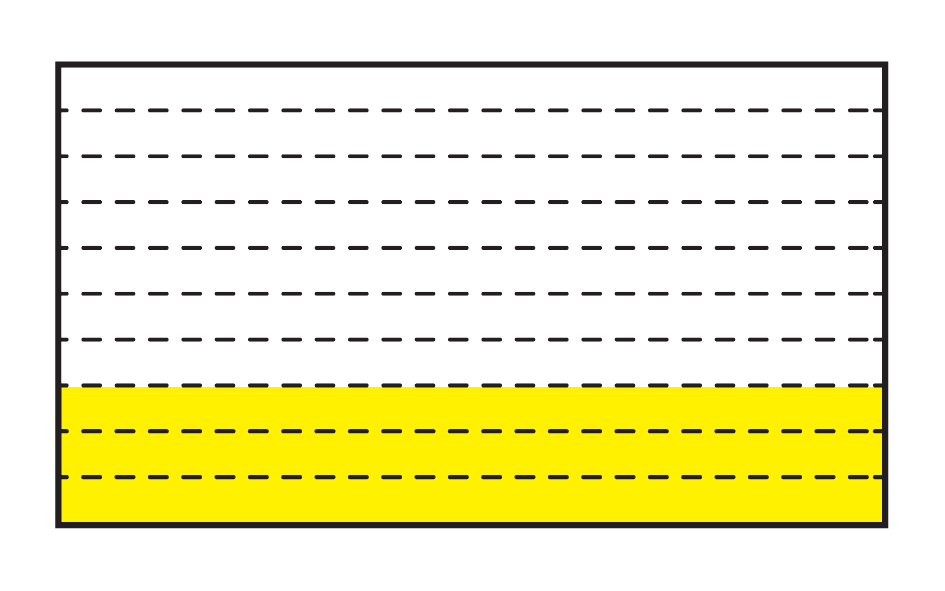
\includegraphics[width=110pt,
keepaspectratio]{../figuras/licao04/ativ2_fig01.png} &  3 &  10 &
$\frac{3}{10}$ \\
      \hline
       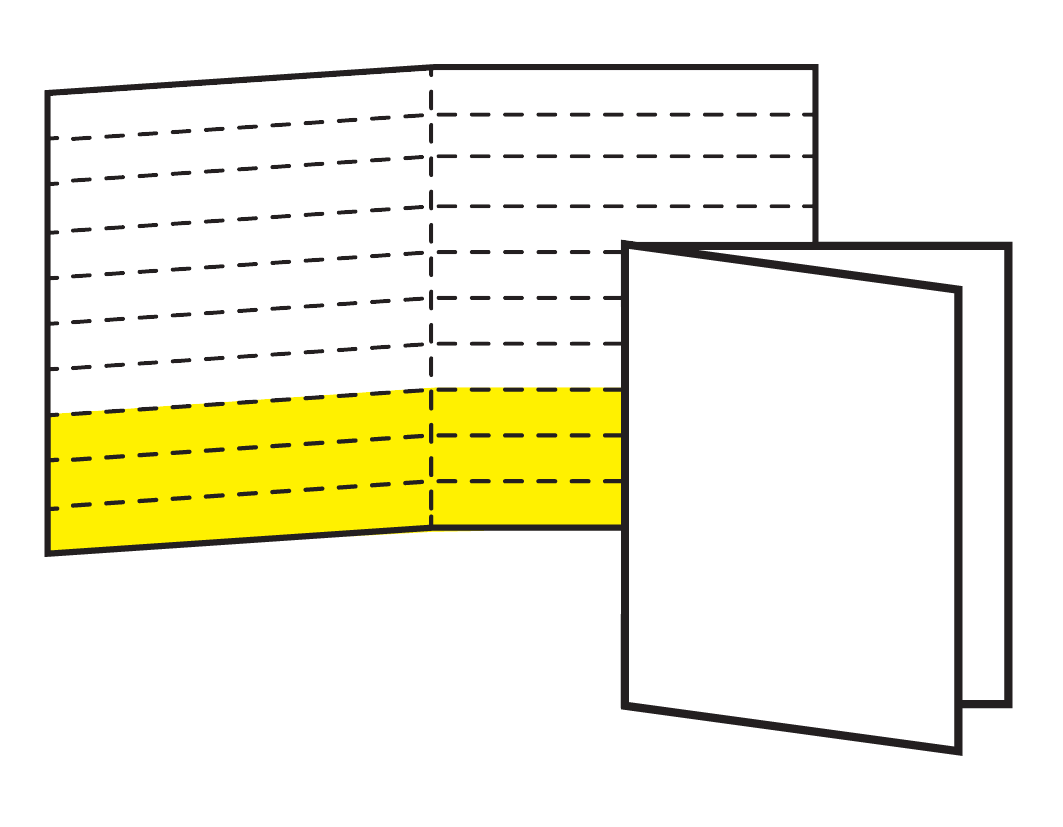
\includegraphics[width=110pt,
keepaspectratio]{../figuras/licao04/ativ2_fig02.png} &  6 &  20 &
$\frac{6}{20}$ \\
      \hline
       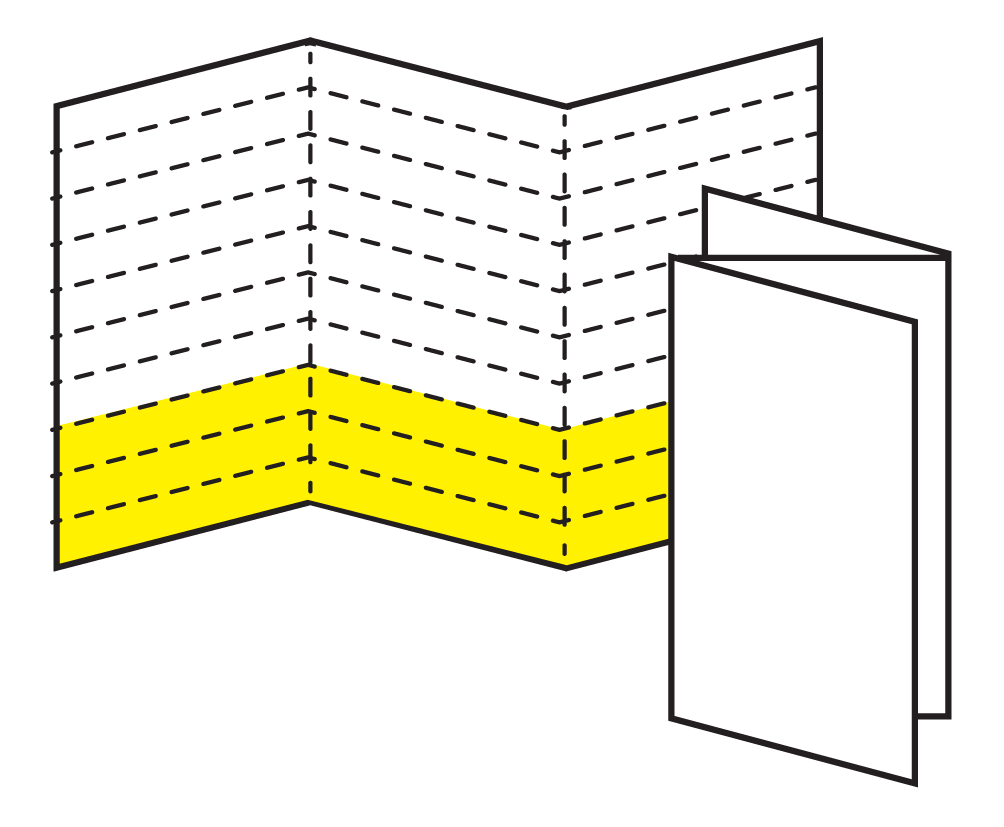
\includegraphics[width=110pt,
keepaspectratio]{../figuras/licao04/ativ2_fig03.png} &  9 &  30 &
$\frac{9}{30}$ \\
      \hline
       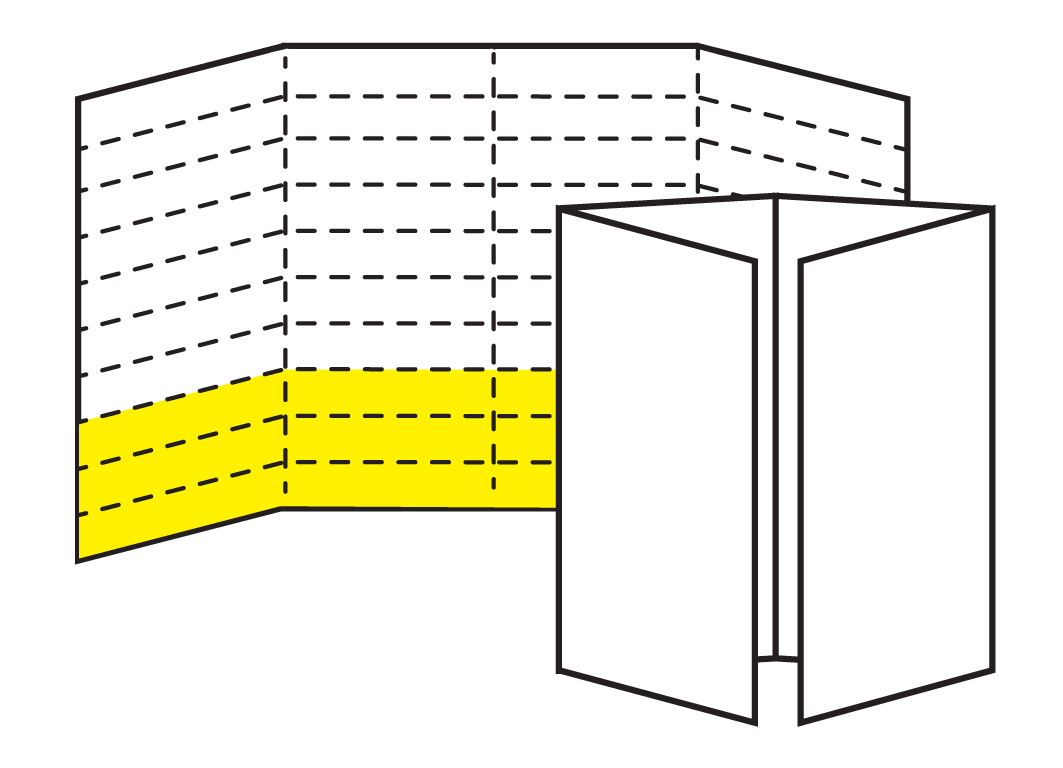
\includegraphics[width=110pt,
keepaspectratio]{../figuras/licao04/ativ2_fig04.png} &  12 &  40 &
$\frac{12}{40}$ \\
      \hline
      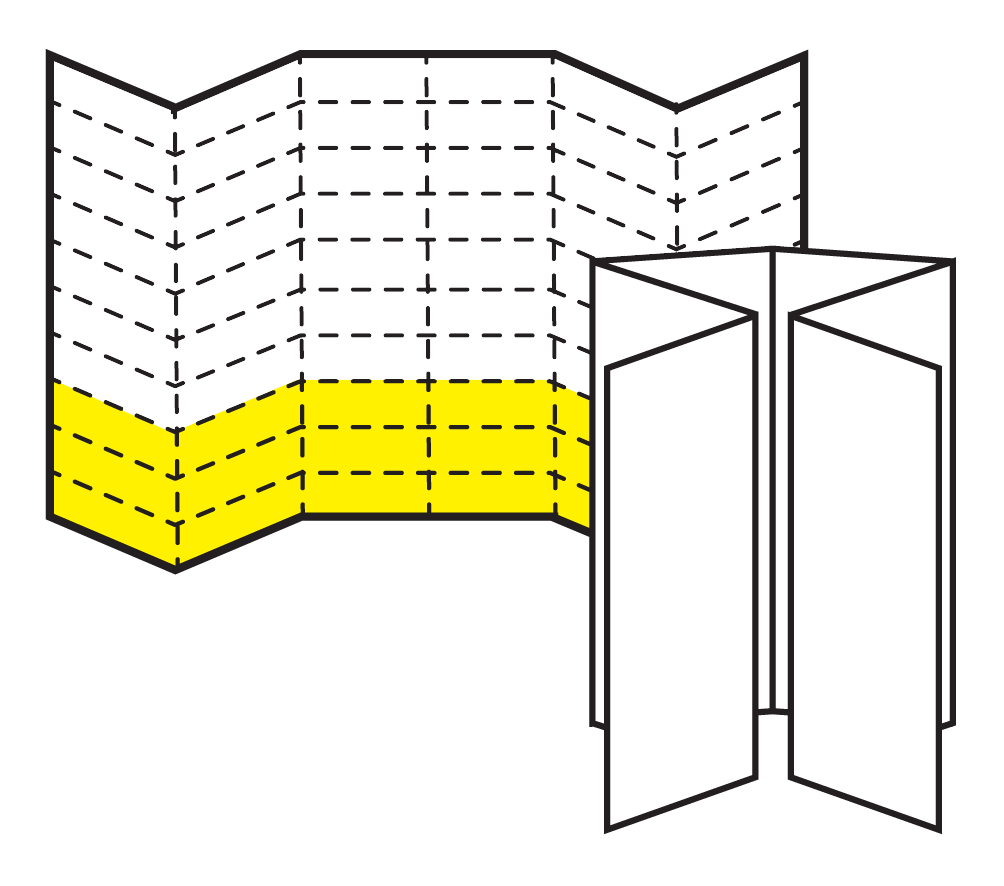
\includegraphics[width=110pt, keepaspectratio]{../figuras/licao04/ativ2_fig05.png}&  18 &  60 &  $\frac{18}{60}$ \\
      \hline
      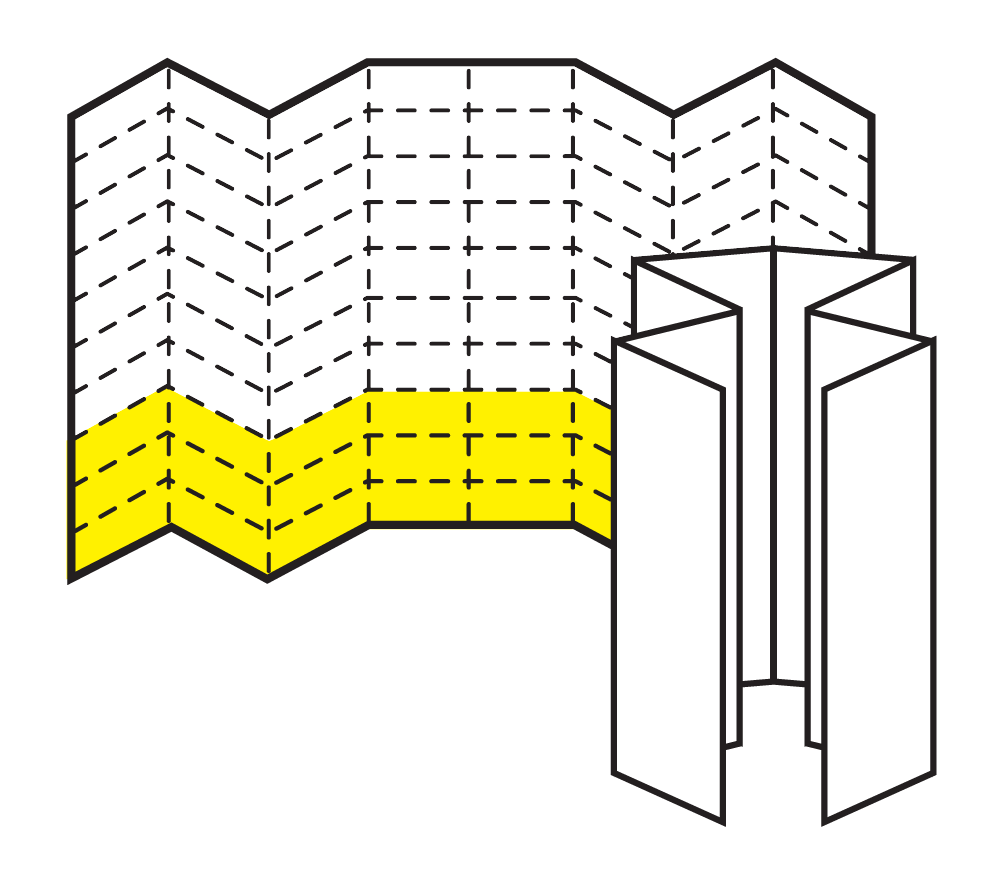
\includegraphics[width=110pt, keepaspectratio]{../figuras/licao04/ativ2_fig06.png}&  24 &  80 &  $\frac{24}{80}$ \\
      \hline
    \end{tabular}

\end{resposta*}

\Bg


\subsection{Atividade 3}


 \noindent {\bf Objetivo específico: Levar o aluno a}
\begin{itemize} %s
    \item       Reconhecer que as frações       $\frac{3}{4}$       e
$\frac{12 \times 3}{12 \times 4}$       são iguais a partir da observação das
representações destas frações em modelos de área sem a contagem um a um das
partes que compõem as subdivisões destas representações.
\end{itemize} %s


  \noindent {\bf Recomendações e sugestões para o desenvolvimento da atividade:}

\begin{itemize} %s
    \item       Recomenda-se que, nesta atividade, os alunos trabalhem
individualmente ou em duplas. No entanto, é fundamental que os alunos sejam
estimulados a explicar o raciocínio realizado.
    \item       O propósito de encobrir as divisões do retângulo é para evitar
que os alunos façam a contagem das partes uma a uma e que, assim, sejam
estimulados a perceber a estrutura multiplicativa       $12 \times 3$       e
   $12 \times 4$       na divisão do retângulo.
    \item       É importante, ao final da atividade, observar para os alunos que
uma mesma parte do retângulo (a área da região pintada de azul) está sendo
descrita por frações com numeradores e denominadores diferentes (isto é, por
frações equivalentes), mas que, não obstante, por expressarem uma mesma
quantidade, estas frações são iguais.
\end{itemize} %s


   \vspace{.1cm}

 \noindent {\bf Classificações:  }\vspace{.1cm}

\begin{itemize} %s
    \item       Heid et al.: Produto: prever
    \item       Nicely, Jr.: Nível 1: reconhecer
    \item       UERJ: Interpretar: compor e decompor
\end{itemize} %s

\begin{resposta*}{Atividade 3}
\begin{enumerate} [\quad a)] %s
    \item             $\frac{3}{4}$.
    \item       Com a nova divisão, o retângulo fica dividido em       $12
\times 4 = 48$       partes, das quais       $12 \times 3 = 36$       está
pintada de azul. Assim, a fração do retângulo que está pintada de azul é igual a
      $\frac{12 \times 3}{12 \times 4} = \frac{36}{48}$.
\end{enumerate} %s

\end{resposta*}

\newpage

\subsection{Atividade 4}

  \noindent {\bf Objetivos específicos: Levar o aluno a }
\begin{itemize} %s
    \item       Comparar frações, em que os denominadores são múltiplos, a
partir de modelos contínuos.
    \item       Introduzir a discusão sobre frações equivalentes.
\end{itemize} %s
\vspace{.15cm}

  \noindent {\bf Recomendações e sugestões para o desenvolvimento da atividade:}

\begin{itemize}
    \item       Recomenda-se que, nesta atividade, os alunos trabalhem
individualmente ou em duplas. No entanto, é fundamental que os alunos sejam
estimulados a explicar o raciocínio realizado.
    \item       Para amparar a reflexão dos alunos, recomenda-se que sejam
feitas cópias das             folhas para reprodução disponíveis no final do
livro.
    \item       Não se recomenda que a nomenclatura       ``frações
equivalentes''       seja introduzida em sala de aula. Por exemplo, pode-se
falar apenas que as frações 1/2 e 2/4 representam a mesma quantidade, e por isso
têm a mesma representação na reta numérica.
    \item       Esta atividade pode desencadear uma discussão com os alunos que
os leve a perceberem que se multiplicamos (dividimos) numerador e denominador de
uma fração pelo mesmo número então é gerada uma fração equivalente à fração
original.
\end{itemize} %s

\begin{resposta*}{Atividade 4}
  Na hora do lanche, João comeu   $\frac{2}{12}$   e Mário   $\frac{4}{12}$   do
bolo. Se os amigos atrasados não tivessem aparecido antes do lanche, João e
Mário teriam comido, cada um,   $\frac{1}{3}$   do bolo. Como   $\frac{1}{3}$
do bolo corresponde a   $4$   fatias do bolo cortado em   $12$   partes iguais,
vê-se que João teria comido mais bolo e Mário teria comido a mesma quantidade de
bolo se seus amigos não tivessem aparecido antes do lanche.
\end{resposta*}

\newpage

\subsection{Atividade 5}

 \noindent {\bf Objetivo específico: Levar o aluno a}
\begin{itemize} %s
    \item       Reconhecer que as frações       $\frac{2}{3}$,
$\frac{4}{6}$       e       $\frac{8}{12}$       são iguais a partir da
observação das representações destas frações em modelos de área circulares.
\end{itemize} %s

  \noindent {\bf Recomendações e sugestões para o desenvolvimento da atividade:}

\begin{itemize} %s
    \item       Recomenda-se que esta atividade seja desenvolvida em grupos de
    $2$       ou       $3$       alunos para que eles possam discutir as
soluções apresentadas, dentro do grupo, durante a condução da atividade.
    \item       Os setores circulares empregados na condução da atividade podem
ser aproveitados da \emph{Atividade 10}       da Lição 1.
    \item       É importante, ao final da atividade, observar para os alunos que
uma mesma parte do círculo (a área da região pintada de cinza) está sendo
descrita por frações com numeradores e denominadores diferentes (isto é, por
frações equivalentes), mas que, não obstante, por expressarem uma mesma
quantidade, estas frações são iguais, não apenas porque por sobreposição parecem
ser a mesma quantidade, mas porque, como na atividade anterior, se cada terço do
círculo for subdividido em 2 e 4 partes iguais, respectivamente, então, de fato,
      $\frac{2}{3}$       =       $\frac{4}{6}$       e       $\frac{2}{3}$
 =       $\frac{8}{12}$.
    \item       Além disso, observaçào análoga cabe para as frações que
completam a terceira coluna da tabela:       $\frac{1}{3}$       =
$\frac{2}{6}$       e       $\frac{1}{3}$       =       $\frac{4}{12}$.
\end{itemize} %s

   \vspace{.1cm}

 \noindent {\bf Classificações:  }\vspace{.1cm}

\begin{itemize} %s
    \item       Heid et al.: Conceito: identificar e descrever
    \item       Nicely, Jr.: Nível 1: reconhecer
    \item       UERJ: Observar: identificar e reconhecer
\end{itemize} %s

\begin{resposta*}{Atividade 5}
\noindent\begin{tabular}{|m{0.10\textwidth}|m{0.08\textwidth}|m{0.08\textwidth}
|m{0.08\textwidth}|}
    \hline
     Tipo da peça &   Quantas cabem na região cinza? &   Juntas, são que fração
do círculo?  &  Fração do círculo não colorida de cinza? \\
    \hline \hline
     $\frac{1}{3}$
\begin{center}
 \begin{tikzpicture}[x=1mm,y=1mm,scale=.5]
  \draw[fill=common] (20,0) arc (0:120:20) -- (0,0)--cycle;
 \end{tikzpicture}
\end{center}
    & $2$ &  $\frac{2}{3}$ &  $\frac{1}{3}$ \\
    \hline
     $\frac{1}{6}$
\begin{center}
\begin{tikzpicture}[x=1mm,y=1mm,scale=.5]
  \draw[fill=light] (20,0) arc (0:60:20) -- (0,0)--cycle;
\end{tikzpicture}
\end{center}
     &  $4$ &  $\frac{4}{6}$ &  $\frac{2}{6}$ \\
    \hline
     $\frac{1}{9}$
\begin{center}
\begin{tikzpicture}[x=1mm,y=1mm,scale=.5]
  \draw[fill=special] (20,0) arc (0:40:20) -- (0,0)--cycle;
\end{tikzpicture}
\end{center}
&   $6$ &  $\frac{6}{9}$ &  $\frac{3}{9}$ \\
    \hline
  \end{tabular}

\end{resposta*}
\Bg
\Bg
\Bg


\begin{multicols}{2}
\subsection{Atividade 6}

 \noindent {\bf Objetivo específico: Levar o aluno a}
\begin{itemize} %s
    \item       Reconhecer que as frações       $\frac{1}{2}$,
$\frac{2}{4}$,       $\frac{3}{6}$,       $\frac{4}{8}$,       $\frac{5}{10}$
   e       $\frac{8}{16}$       são iguais a partir da observação das
representações destas frações em modelos de área retangulares.
\end{itemize} %s


  \noindent {\bf Recomendações e sugestões para o desenvolvimento da atividade:}

\begin{itemize} %s
    \item       Recomenda-se que esta atividade seja desenvolvida em grupos de
    $2$       ou       $3$       alunos para que eles possam discutir as
soluções apresentadas, dentro do grupo, durante a condução da atividade.
    \item       É importante, ao final da atividade, observar para os alunos que
uma mesma parte do retângulo (a região colorida de cinza) está sendo descrita
por frações com numeradores e denominadores diferentes (isto é, por frações
equivalentes) mas que, não obstante, por expressarem uma mesma quantidade, são
frações iguais.
\end{itemize} %s


  Esta atividade possui     folhas para reprodução disponíveis no final do
livro.

   \vspace{.1cm}

 \noindent {\bf Classificações:  }\vspace{.1cm}

\begin{itemize} %s
    \item       Heid et al.: Conceito: identificar e descrever
    \item       Nicely, Jr.: Nível 1: reconhecer
    \item       UERJ: Observar: identificar e reconhecer
\end{itemize} %s


 \vspace*{\fill}
\columnbreak

\begin{resposta*}{Atividade 6}
  {\bf PARTE 1}


\begin{center}
  \begin{tabular}{|m{.19\textwidth}|m{.12\textwidth}|m{.12\textwidth}|}
    \hline
      \centering Retângulo  &   Número de partes em se encontra dividido  &
Cada parte é que fração do retângulo?  \\
    \hline \hline
   \centering
    \begin{tikzpicture}[x=1mm,y=1mm,scale=.5]
\draw[fill=light] (0,0) rectangle (60,12);
\draw (30,0) -- (30,12);
    \end{tikzpicture}   &   \centering $2$  & \parbox[t][1.3
cm][c]{.25\textwidth}{ $\dfrac{1}{2}$}  \\
    \hline
 \centering  \begin{tikzpicture}[x=1mm,y=1mm,scale=.5]
\draw[fill=pink] (0,0) rectangle (60,12);
\foreach \x in {1,2} \draw (\x*60/3,0) -- (\x*60/3,12);
    \end{tikzpicture}        & \centering       3  & \parbox[t][1.3
cm][c]{1cm}{$\frac{1}{3}$ } \\
    \hline
    \centering  \begin{tikzpicture}[x=1mm,y=1mm,scale=.5]
\draw[fill=special] (0,0) rectangle (60,12);
\foreach \x in {1,2,3} \draw (\x*60/4,0) -- (\x*60/4,12);
    \end{tikzpicture}        & \centering   4  &  \parbox[t][1.3
cm][c]{1cm}{$\frac{1}{4}$}  \\
    \hline
 \centering  \begin{tikzpicture}[x=1mm,y=1mm,scale=.5]
\draw[fill=attention] (0,0) rectangle (60,12);
\foreach \x in {1,...,4} \draw (\x*60/5,0) -- (\x*60/5,12);
    \end{tikzpicture}        & \centering  5  & \parbox[t][1.3
cm][c]{1cm}{$\frac{1}{5}$}  \\
    \hline
 \centering  \begin{tikzpicture}[x=1mm,y=1mm,scale=.5]
\draw[fill=common] (0,0) rectangle (60,12);
\foreach \x in {1,...,5} \draw (\x*60/6,0) -- (\x*60/6,12);
    \end{tikzpicture}        & \centering   6  & \parbox[t][1.3
cm][c]{1cm}{$\frac{1}{6}$}  \\
    \hline
  \centering  \begin{tikzpicture}[x=1mm,y=1mm,scale=.5]
\draw[fill=CornflowerBlue] (0,0) rectangle (60,12);
\foreach \x in {1,...,6} \draw (\x*60/7,0) -- (\x*60/7,12);
    \end{tikzpicture}        & \centering    7  & \parbox[t][1.3
cm][c]{1cm}{$\frac{1}{7}$}  \\
    \hline
 \centering  \begin{tikzpicture}[x=1mm,y=1mm,scale=.5]
\draw[fill=dark] (0,0) rectangle (60,12);
\foreach \x in {1,...,7} \draw (\x*60/8,0) -- (\x*60/8,12);
    \end{tikzpicture}        & \centering  8  & \parbox[t][1.3
cm][c]{1cm}{$\frac{1}{8}$}  \\
    \hline
 \centering  \begin{tikzpicture}[x=1mm,y=1mm,scale=.5]
\draw[fill=Fuchsia] (0,0) rectangle (60,12);
\foreach \x in {1,...,8} \draw (\x*60/9,0) -- (\x*60/9,12);
    \end{tikzpicture}        & \centering   9  & \parbox[t][1.3
cm][c]{1cm}{$\frac{1}{9}$}  \\
    \hline
 \begin{tikzpicture}   [x=1mm,y=1mm,scale=.5]
 \draw[fill=NavyBlue] (0,0) rectangle (60,12);
 \foreach \x in {1,...,9} \draw (\x*60/10,0) -- (\x*60/10,12);
     \end{tikzpicture}        & \centering     10  & \parbox[t][1.3
cm][c]{1cm}{$\frac{1}{10}$}  \\
    \hline
\begin{tikzpicture}   [x=1mm,y=1mm,scale=.5]
    \draw[fill=BlueViolet] (0,0) rectangle (60,12);
\foreach \x in {1,...,15} \draw (\x*60/16,0) -- (\x*60/16,12);
    \end{tikzpicture}        & \centering  16  & \parbox[t][1.3
cm][c]{1cm}{$\frac{1}{16}$}  \\
    \hline
 \end{tabular}
\end{center}

  \clearpage

  {\bf PARTE 2 }

\noindent\begin{tabular}{|m{.15\textwidth}|m{.065\textwidth}|m{.07\textwidth}|m{
.075\textwidth}|}
 \hline
 \centering Tipo da peça &   Quantas cabem na região cinza? &   Juntas, são que
fração do retângulo do encarte?  &  Fração do encarte não colorida de cinza? \\
    \hline    \hline
 \begin{tikzpicture}[x=1mm, y=1mm, scale=.5]
% Fita de largura 1/2
\draw[fill=light] (0,0) rectangle (100/2,10);
\end{tikzpicture} &  \parbox[t][1.3 cm][c]{1cm}{$1$} &  $\frac{1}{2}$ &
$\frac{1}{2}$ \\
    \hline
\centering  \begin{tikzpicture}[x=1mm, y=1mm, scale=.5]
% Fita rosa de largura 1/4
\draw[fill=pink] (0,0) rectangle (100/4,10);
\end{tikzpicture}
        &  \parbox[t][1.3 cm][c]{1cm}{ $2$ }  &  $\frac{2}{4}$ &  $\frac{2}{4}$
\\
    \hline
 \centering \begin{tikzpicture}[x=1mm, y=1mm, scale=.5]
% Fita rosa de largura 1/6
\draw[fill=special] (0,0) rectangle (100/6,10);
\end{tikzpicture}    &  \parbox[t][1.3 cm][c]{1cm}{ $3$ } &  $\frac{3}{6}$ &
$\frac{3}{6}$ \\
    \hline
\centering \begin{tikzpicture}[x=1mm, y=1mm, scale=.5]
% Fita rosa de largura 1/8
\draw[fill=attention] (0,0) rectangle (100/8,10);
\end{tikzpicture}     &  \parbox[t][1.3 cm][c]{1cm}{   $4$} &  $\frac{4}{8}$ &
$\frac{4}{8}$ \\
    \hline
\centering \begin{tikzpicture}[x=1mm, y=1mm, scale=.5]
% Fita rosa de largura 1/10
\draw[fill=common] (0,0) rectangle (100/10,10);
\end{tikzpicture}     &  \parbox[t][1.3 cm][c]{1cm}{ $5$ } &  $\frac{5}{10}$ &
$\frac{5}{10}$ \\
    \hline
\centering \begin{tikzpicture}[x=1mm, y=1mm, scale=.5]
% Fita rosa de largura 1/16
\draw[fill=CornflowerBlue] (0,0) rectangle (100/16,10);
\end{tikzpicture}     &  \parbox[t][1.3 cm][c]{1cm}{ $8$ } &  $\frac{8}{16}$ &
$\frac{8}{16}$ \\
    \hline
  \end{tabular}

\end{resposta*}

\Bg

\subsection{Atividade 7}

 \noindent {\bf Objetivo específico: Levar o aluno a}
\begin{itemize} %s
    \item       Reconhecer que, para cada       $0 \leq i \leq 3$, as frações
   $\frac{i}{3}$,       $\frac{2 \times i}{2 \times 3 }$,       $\frac{3 \times
i}{3 \times 3}$       e       $\frac{4 \times i}{4 \times 3}$       são iguais a
partir da observação das representações destas frações na reta numérica.
\end{itemize} %s


  \noindent {\bf Recomendações e sugestões para o desenvolvimento da atividade:}

\begin{itemize} %s
    \item       Recomenda-se que, nesta atividade, os alunos trabalhem
individualmente ou em duplas. No entanto, é fundamental que os alunos sejam
estimulados a explicar o raciocínio realizado.
    \item       Nas retas numéricas apresentadas, as origens estão alinhadas e
as unidades correspondem a segmentos unitários congruentes, o que garante que
uma fração associada a um determinado ponto em uma reta seja a mesma fração nos
pontos correspondentes nas demais retas.
    \item       Caso seus alunos não percebam, aponte para o fato de que as
segunda, terceira e quarta retas numéricas são obtidas por meio de subdivisões
dos terços da primeira reta numérica em duas, três e quatro partes iguais,
respectivamente. Para resolver o item c) desta atividade, se faz necessário
dividir cada terço em cinco partes iguais.
    \item       É importante, ao final da atividade, observar para os alunos
que, nesta atividade, cada ponto marcado na reta numérica está sendo descrito
por frações com numeradores e denominadores diferentes (isto é, por frações
equivalentes) mas que, não obstante, por corresponderem ao mesmo ponto da reta
numérica, estas frações são iguais.
\end{itemize} %s


   \vspace{.1cm}

 \noindent {\bf Classificações:  }\vspace{.1cm}

\begin{itemize} %s
    \item       Heid et al.: Conceito: identificar e descrever
    \item       Nicely, Jr.: Nível 1: reconhecer
    \item       UERJ: Observar: identificar e reconhecer
\end{itemize} %s


  Para o item c):
\begin{itemize} %s
    \item       Heid et al.: Produto: gerar
    \item       Nicely, Jr.: Nível 3: comparar
    \item       UERJ: Interpretar: discriminar
\end{itemize} %s

\begin{resposta*}{Atividade 7}

\noindent a)

 \noindent \begin{tikzpicture}[x=45mm,y=45mm, scale=.53]
  \draw (0,0) -- (3,0);
  \foreach \x in {0,...,3}{ \draw (\x,-3pt) -- (\x, 3pt);  \node[above] at (\x,3pt) {\x}; }

  \foreach \x in {0,1,...,9}{
  \draw (\x/3,-2pt) -- (\x/3, 2pt);
  \node[below] at (\x/3,-2 pt) {$\frac{\x}{3}$};
  \draw[dotted] (\x/3,-35pt) -- (\x/3, -60pt);
  }

  \fill[common] (1+1/3,0) circle (2pt);

  \begin{scope}[shift={(0,-80pt)}]
  \draw (0,0) -- (3,0);
  \foreach \x in {0,...,3}{
  \draw (\x,-3pt) -- (\x, 3pt);
  \node[above] at (\x,3pt) {\x};
  }

  \foreach \x in {0,2,...,18}{
  \draw (\x/6,-2pt) -- (\x/6, 2pt);
  \node[below] at (\x/6,-2 pt) { $\frac{\x}{6}$ };
  \draw[dotted] (\x/6,-35pt) -- (\x/6, -60pt);
  }

  \foreach \x in {0,.333,...,6}{
  \draw (\x/2,-2pt) -- (\x/2, 2pt);}


  \fill[common] (1+1/3,0) circle (2pt);

  \end{scope}


  \begin{scope}[shift={(0,-160pt)}]
  \draw (0,0) -- (3,0);
  \foreach \x in {0,...,3}{
  \draw (\x,-3pt) -- (\x, 3pt);
  \node[above] at (\x,3pt) {\x};}

  \foreach \x in {0,3,...,27}{
  \draw (\x/9,-2pt) -- (\x/9, 2pt);
  \node[below] at (\x/9,-2 pt) {$\frac{\x}{9}$};
  \draw[dotted] (\x/9,-35pt) -- (\x/9, -60pt);
  }

  \foreach \x in {0,.333,...,9}{
  \draw (\x/3,-2pt) -- (\x/3, 2pt);}



  \fill[common] (1+1/3,0) circle (2pt);

  \end{scope}

  \begin{scope}[shift={(0,-240pt)}]
  \draw (0,0) -- (3,0);
  \foreach \x in {0,...,3}{
  \draw (\x,-3pt) -- (\x, 3pt);
  \node[above] at (\x,3pt) {\x};}

  \foreach \x in {0,4,...,36}{
  \draw (\x/12,-2pt) -- (\x/12, 2pt);
  \node[below] at (\x/12,-2 pt) {$\frac{\x}{12}$};
  %\draw[dotted] (\x,-30pt) -- (\x, -60pt);
  }

  \foreach \x in {0,.333,...,12}{
  \draw (\x/4,-2pt) -- (\x/4, 2pt);}

  \fill[common] (1+1/3,0) circle (2pt);

  \end{scope}
 \end{tikzpicture}

\noindent b) $\frac{4}{3} = \frac{8}{6} = \frac{12}{9} = \frac{16}{12}$.

\noindent c) No item b) foi estabelecido que o ponto azul corresponde a fração
$\frac{4}{3}$       pois, ao se justapor 4 segmentos que são       $\frac{1}{3}$
      do segmento unitário (que está, aqui, servindo como unidade) a partir da
origem       $0$, este ponto é a outra extremidade desta justaposição. Agora, ao
se subdividir estes 4 segmentos que são       $\frac{1}{3}$       do segmento
unitário em 5 partes iguais, obtêm-se 20 segmentos justapostos que são
$\frac{1}{15}$       do segmento unitário. Sendo o ponto azul extremo desta
justaposição, segue-se que ele corresponde a fração       $\frac{20}{15}$.



\noindent \begin{tikzpicture}[x=45mm,y=45mm, scale=.53]
  \draw (0,0) -- (3,0);
  \foreach \x in {0,...,3}{ \draw (\x,-3pt) -- (\x, 3pt);  \node[above] at (\x,3pt) {\x}; }

  \foreach \x in {0,1,...,9}{
  \draw (\x/3,-2pt) -- (\x/3, 2pt);
  \node[below] at (\x/3,-2 pt) {$\frac{\x}{3}$};
  \draw[dotted] (\x/3,-35pt) -- (\x/3, -60pt);
  }

  \fill[common] (1+1/3,0) circle (2pt);

  \begin{scope}[shift={(0,-80pt)}]
  \draw (0,0) -- (3,0);
  \foreach \x in {0,...,3}{
  \draw (\x,-3pt) -- (\x, 3pt);
  \node[above] at (\x,3pt) {\x};
  }

  \foreach \x in {0,5,...,45}{
  \node[below] at (\x/15,-2 pt) { $\frac{\x}{15}$ };
  %\draw[dotted] (\x/15,-35pt) -- (\x/15, -60pt);
  }

  \foreach \x in {0,1,...,45}{
  \draw (\x/15,-2pt) -- (\x/15, 2pt);}


  \fill[common] (1+1/3,0) circle (2pt);

  \end{scope}
\end{tikzpicture}

\end{resposta*}

\Bg
\Bg

\subsection{Atividade 8}

 \noindent {\bf Objetivo específico: Levar o aluno a}
\begin{itemize} %s
    \item       Determinar uma fração igual a uma dada fração com denominador
especificado a partir da observação das representações destas frações em
diversos modelos de frações, incluindo a reta numérica.
\end{itemize} %s

  \noindent {\bf Recomendações e sugestões para o desenvolvimento da atividade:}

\begin{itemize} %s
    \item       Recomenda-se que esta atividade seja desenvolvida em grupos de 3
alunos (cada aluno do grupo poderá usar um modelo diferente para obter a fração
solicitada).
    \item       É importante, ao final da atividade, observar para os alunos que
uma mesma parte em cada modelo de área e um mesmo ponto na reta numérica estão
sendo descritos por frações com numeradores e denominadores diferentes (isto é,
por frações equivalentes) mas que, não obstante, estas frações são iguais por
expressarem uma mesma quantidade ou por serem representadas por um mesmo ponto
na reta numérica.
\end{itemize} %s

   \vspace{.1cm}

 \noindent {\bf Classificações:  }\vspace{.1cm}

\begin{itemize} %s
    \item       Heid et al.: Produto: gerar
    \item       Nicely, Jr.: Nível 5: aplicar
    \item       UERJ: Interpretar: discriminar
\end{itemize} %s

\begin{resposta*}{Atividade 8}
\begin{enumerate} [\quad a)] %s
    \item       Tomando um círculo como unidade, o dividimos em       $4$
partes iguais e tomamos       $5$       cópias de uma parte para obter
$\frac{5}{4}$       da unidade. Dividindo cada uma das       $5$       cópias em
      $3$       partes iguais, obtemos então       $15$       cópias de
$\frac{1}{12}$       da unidade. Portanto,       $\frac{5}{4} = \frac{15}{12}$.



\noindent \begin{tikzpicture}[x=1mm,y=1mm, scale=1.45]
 \draw[fill=common, fill opacity=.3] (0,0) circle (5);
 \node at (0,7) {Unidade};


 \begin{scope}[xshift=45]
 \draw[->] (-10,0) -- (-6,0);
 \node[text width=23 mm] at (-8,-11) {Divide-se a unidade em 4 partes iguais.};


 \draw[fill=common, fill opacity=.3] (0,0) circle (5);
 \draw (90:5) -- (-90:5);
 \draw (0:5) -- (180:5);

 \draw[->] (6,0) -- (10,0);
 \node[text width=22 mm] at (10,-11) {Uma parte corresponde a um quarto.};

 \draw[fill=common, fill opacity=.3, xshift=32, yshift=-5] (0:5) arc (0:90:5) -- (0,0)--cycle;

 \end{scope}

 \begin{scope}[ yshift=-26mm]

 \node[text width=30 mm] at (3,-12) {Junta-se 5 cópias de uma parte para obter cinco quartos.};

 \draw[fill=common, fill opacity=.3] (0,0) circle (5);
 \draw (90:5) -- (-90:5);
 \draw (0:5) -- (180:5);

 \draw[fill=common, fill opacity=.3, xshift=6mm, yshift=-5] (0:5) arc (0:90:5) -- (0,0)--cycle;


 \begin{scope}[xshift=65]
  \draw[->] (-10,0) -- (-6,0);
 \node[text width=33 mm] at (4,-14) {Divide-se cada cópia em 3 partes iguais obtendo 15 cópias de um doze avos.};

 \draw[fill=common, fill opacity=.3] (0,0) circle (5);
 \foreach \x in {0,30,...,150}{ \draw (\x:5) -- (\x:-5);}

 \draw[fill=common, fill opacity=.3, xshift=6mm, yshift=-5] (0:5) arc (0:90:5) -- (0,0)--cycle;
 \foreach \x in {30,60}{ \draw[xshift=6mm, yshift=-5] (\x:5) -- (0,0);}
 \end{scope}
 \end{scope}

 \end{tikzpicture}

    \item       Tomando um quadrado como unidade, o dividimos em       $4$
partes iguais e tomamos       $5$       cópias de uma parte para obter
$\frac{5}{4}$       da unidade. Dividindo cada uma das       $5$       cópias em
      $3$       partes iguais, obtemos então       $15$       cópias de
$\frac{1}{12}$       da unidade. Portanto,       $\frac{5}{4} = \frac{15}{12}$.

\noindent \begin{tikzpicture}[x=1mm,y=1mm,scale=1.45]
           \draw[fill=common, fill opacity=.3] (0,0) rectangle (10,10);
	   \node at (5,12) {Unidade};


 \begin{scope}[xshift=45]
 \draw[->] (-5,5) -- (-1,5);
 \node[text width=23 mm] at (-4,-8) {Divide-se a unidade em 4 partes iguais.};

 \draw[fill=common, fill opacity=.3] (0,0) rectangle (10,10);
 \draw (0,5) -- (10,5);
 \draw (5,0) -- (5,10);

 \draw[->] (11,5) -- (15,5);
 \node[text width=22 mm] at (14,-8) {Uma parte corresponde a um quarto.};

 \draw[fill=common, fill opacity=.3, xshift=16mm, yshift=2.5mm] (0,0) rectangle (5,5);

 \end{scope}

 \begin{scope}[ yshift=-27mm]

 \node[text width=30 mm] at (9,-8) {Junta-se 5 cópias de uma parte para obter cinco quartos.};

 \draw[fill=common, fill opacity=.3] (0,0) rectangle (10,10);
 \draw (0,5) -- (10,5);
 \draw (5,0) -- (5,10);

 \draw[fill=common, fill opacity=.3, xshift=11mm, yshift=5mm] (0,0) rectangle (5,5);

 \draw[->] (17,5) -- (21,5);
 \begin{scope}[xshift=62]

  \node[text width=32 mm] at (10,-9) {Divide-se cada cópia em 3 partes iguais obtendo 15 cópias de um doze avos.};

 \draw[fill=common, fill opacity=.3] (0,0) rectangle (10,10);
 \foreach \x in {10,20,...,50} \draw (\x/6,0) -- (\x/6,10);
 \draw (0,5) -- (10,5);

 \draw[fill=common, fill opacity=.3, xshift=11mm, yshift=5mm] (0,0) rectangle (5,5);
 \foreach \x in {10,20} \draw[xshift=11mm, yshift=5mm] (\x/6,0) -- (\x/6,5);
 \end{scope}
 \end{scope}

          \end{tikzpicture}


\end{enumerate} %s
% \end{resposta*}
%
% \pagebreak
% \end{multicols}
\begin{enumerate}[a)]

    \item[c)] Após marcar os números       $0$       e       $1$       na reta
numérica, dividimos o segmento unitário (aquele de extremidades em       $0$
  e       $1$) em       $4$       partes iguais. Cada parte é um segmento que
corresponde a       $\frac{1}{4}$       da unidade. Ao se justapor       $5$
  segmentos que são       $\frac{1}{4}$       da unidade a partir da origem 0, a
fração       $\frac{5}{4}$       corresponde ao ponto que é a outra extremidade
desta justaposição. Agora, ao se subdividir estes 5 segmentos que são
$\frac{1}{4}$       da unidade em 5 partes iguais, obtêm-se       $15$
segmentos justapostos que são       $\frac{1}{12}$       da unidade. O ponto que
corresponde a       $\frac{5}{4}$       é ainda extremo desta justaposição e,
portanto, que ele corresponde também a fração       $\frac{15}{12}$.



\begin{center}

 \begin{tikzpicture}[x=21mm,y=21mm]
  \draw (0,0) -- (3,0);
  \foreach \x in {0,...,3}{ \draw (\x,-3pt) -- (\x, 3pt);  \node[above] at (\x,3pt) {\x}; }

  \foreach \x in {0,1,...,5}{
  \draw (\x/4,-2pt) -- (\x/4, 2pt);
  \node[below] at (\x/4,-2 pt) {$\frac{\x}{4}$};}
  \draw[dotted] (5/4,-.3) -- (5/4, -.6);


  \fill[common] (5/4,0) circle (2pt);

  \begin{scope}[shift={(0,-.7)}]
  \draw (0,0) -- (3,0);
  \foreach \x in {0,...,3}{
  \draw (\x,-3pt) -- (\x, 3pt);
  \node[above] at (\x,3pt) {\x};
  }

  \foreach \x in {0,3,...,15}{
  \node[below] at (\x/12,-2 pt) { $\frac{\x}{12}$ };
  %\draw[dotted] (\x/15,-35pt) -- (\x/15, -60pt);
  }

  \foreach \x in {0,1,...,15}{
  \draw (\x/12,-2pt) -- (\x/12, 2pt);}


  \fill[common] (1+1/4,0) circle (2pt);

  \end{scope}
\end{tikzpicture}

\end{center}
\end{enumerate}
\end{resposta*}
% \newpage
\Bg
% \begin{multicols}{2}
\subsection{Atividade 9}

 \noindent {\bf Objetivo específico: Levar o aluno a}
\begin{itemize} %s
    \item       Determinar uma fração igual a uma dada fração irredutível com
denominador especificado.
\end{itemize} %s


  \noindent {\bf Recomendações e sugestões para o desenvolvimento da atividade:}


\begin{itemize} %s
    \item       Recomenda-se que, nesta atividade, os alunos trabalhem
individualmente ou em duplas. No entanto, é fundamental que os alunos sejam
estimulados a explicar o raciocínio realizado.
    \item       Espera-se, principalmente nos Itens c e d, que os alunos
consigam obter a fração solicitada usando a propriedade que       $\frac{m
\times a}{m \times b}$       é equivalente a       $\frac{a}{b}$       e sem
recorrer a desenhos de modelos de área de frações.
\end{itemize} %s


   \vspace{.1cm}

 \noindent {\bf Classificações:  }\vspace{.1cm}

\begin{itemize} %s
    \item       Heid et al.: Produto: gerar
    \item       Nicely, Jr.: Nível 3: comparar
    \item       UERJ: Interpretar: discriminar
\end{itemize} %s


\begin{resposta*}{Atividade 9}
\begin{enumerate} [\quad a)] %s
    \item       Como       $6 = 2 \times 3$, segue-se que       $\frac{7}{3} =
\frac{2 \times 7}{2 \times 3} = \frac{14}{6}$.
    \item       Como       $21 = 7 \times 3$, segue-se que       $\frac{7}{3} =
\frac{7 \times 7}{7 \times 3} = \frac{49}{21}$.
    \item       Como       $123 = 41 \times 3$, segue-se que       $\frac{7}{3}
= \frac{41 \times 7}{41 \times 3} = \frac{287}{123}$.
    \item       Como       $210 = 70 \times 3$, segue-se que       $\frac{7}{3}
= \frac{70 \times 7}{70 \times 3} = \frac{490}{210}$.
\end{enumerate} %s
\end{resposta*}

\subsection{Atividade 10}

 \noindent {\bf Objetivo específico: Levar o aluno a}
\begin{itemize} %s
    \item       Determinar uma fração igual a uma dada fração com numerador ou
denominador especificados.
\end{itemize} %s

\noindent {\bf Recomendações e sugestões para o desenvolvimento da atividade:}
\begin{itemize} %s
    \item       Recomenda-se que, nesta atividade, os alunos trabalhem
individualmente. No entanto, é fundamental que os alunos sejam estimulados a
explicar o raciocínio realizado.
    \item       Espera-se que, neste estágio, os alunos consigam obter as
respostas usando a propriedade que       $\frac{m \times a}{m \times b}$       é
equivalente a       $\frac{a}{b}$       e sem recorrer a desenhos de modelos de
área de frações.
    \item       Observe que, no item (e), não existe um número natural       $n$
      tal que       $6 \times n = 9$. Para resolver o item, o aluno pode usar o
resultado do item (d) e substituir       $\frac{9}{12}$       por
$\frac{3}{4}$       e proceder com o exercício. A mesma observação aplica-se ao
item (f).
    \item       Observe para seus alunos que os Itens (e) e (f) são exemplos de
frações iguais para os quais não é possível obter uma fração multiplicando-se o
numerador e o denominador da outra por um mesmo número natural.
\end{itemize} %s


   \vspace{.1cm}

 \noindent {\bf Classificações:  }\vspace{.1cm}

\begin{itemize} %s
    \item       Heid et al.: Produto: gerar
    \item       Nicely, Jr.: Nível 3: comparar
    \item       UERJ: Interpretar: discriminar
\end{itemize} %s


\begin{resposta*}{Atividade 10}
\begin{enumerate} [\quad a)] %s
    \item       Uma vez que       $6 = 2 \times 3$, então       $\frac{5}{3} =
\frac{2 \times 5}{2 \times 3} = \frac{10}{6}$. Logo,       $\square$       deve
ser preenchido com       $10$.
    \item       Uma vez que       $6 = 3 \times 2$, então       $\frac{2}{3} =
\frac{3 \times 2}{3 \times 3} = \frac{6}{9}$. Logo,       $\square$       deve
ser preenchido com       $9$.
    \item       Uma vez que       $12 = 4 \times 3$       e       $8 = 4 \times
2$, então       $\frac{8}{12} = \frac{4 \times 2}{4 \times 3} = \frac{2}{3}$.
Logo,       $\square$       deve ser preenchido com       $2$.
    \item       Uma vez que       $9 = 3 \times 3$       e       $12 = 3 \times
4$, então       $\frac{9}{12} = \frac{3 \times 3}{3 \times 4} = \frac{3}{4}$.
Logo,       $\square$       deve ser preenchido com       $4$.
    \item       Pelo item d,       $\frac{9}{12} = \frac{3}{4}$. Uma vez que
  $6 = 2 \times 3$, então       $\frac{3}{4} = \frac{2 \times 3}{2 \times 4} =
\frac{6}{8}$. Logo,       $\square$       deve ser preenchido com       $8$.
    \item       Pela solução do item e,       $\square$       deve ser
preenchido com       $9$.
\end{enumerate} %s

\end{resposta*}



\subsection{Atividade 11}

 \noindent {\bf Objetivo específico: Levar o aluno a}
\begin{itemize} %s
    \item       Usar igualdade de frações para calcular o numerador de uma das
frações em uma situação contextualizada.
\end{itemize} %s

  \noindent {\bf Recomendações e sugestões para o desenvolvimento da atividade:}

\begin{itemize} %s
    \item       Recomenda-se que, nesta atividade, os alunos trabalhem
individualmente ou em duplas. No entanto, é fundamental que os alunos sejam
estimulados a explicar o raciocínio realizado.
\end{itemize} %s

 \vspace{.1cm}

 \noindent {\bf Classificações:  }\vspace{.1cm}

\begin{itemize} %s
  \item     Heid et al.: Produto: prever
  \item     Nicely, Jr.: Nível 6: analisar
  \item     UERJ: Interpretar: explicar
\end{itemize} %s

\begin{resposta*}{Atividade 11}
  As 17 marcações no copo do seu colega divide a capacidade do copo em 16 partes
iguais. Quantas destas partes correspondem a   $\frac{3}{4}$   da capacidade do
copo (que é fração da capacidade do copo que está preenchida com suco)? Para
responder a esta pergunta, devemos calcular o numerador de uma fração de
denominador 16 que seja igual a   $\frac{3}{4}$  , isto é, devemos preencher
$\square$   com um número tal que

  $\frac{3}{4} = \frac{\square}{16}$.

  Como   $16 = 4 \times 4$  , segue-se que

  $\frac{3}{4} = \frac{4 \times 3}{4 \times 4} = \frac{12}{16}$.

  Assim, não necessárias   $12$   partes de   $\frac{1}{16}$   da capacidade do
copo. Consequentemente,
  13 níveis do copo do seu colega devem ser preenchidos com suco de laranja para
que ele fique com a mesma quantidade suco de laranja que você.


\begin{center}
 \begin{tikzpicture}[scale=0.5, x=1cm,y=1cm]

% Definição do eixo vertical das elipses
\def\EixoM{0.3}

% colorindo o primeiro cilindro
\fill[light, opacity=1] (2,0) ellipse (2 and \EixoM);
\fill[light,fill opacity=.8] (0,0) rectangle (4,3);
\fill[fill=light,fill opacity=1] (2,3) ellipse (2 and \EixoM);


\pgfpathmoveto{\pgfpoint{0 cm}{0 cm}}
\pgfpatharc{-180}{0}{2cm and \EixoM cm}
\pgfusepath{draw}

\draw (2,4) ellipse (2 and \EixoM);
\draw (0,0) -- (0,4);
\draw (4,0) -- (4,4);

% shift vertical nos arcos de elipse definido por \y
\foreach \y in {0,.25,...,4}{
\pgfpathmoveto{\pgfpoint{0 cm}{\y cm}}
\pgfpatharc{-180}{-130}{2cm and \EixoM cm}
\color{Green}
\pgfusepath{draw}}
\end{tikzpicture}
\end{center}

 \end{resposta*}




\subsection{Atividade 12}

 \noindent {\bf Objetivo específico: Levar o aluno a}
\begin{itemize} %s
    \item       Reconhecer que, dada uma fração       $p = \frac{n}{d}$, existe
um quantidade finita de frações da forma       $\frac{k}{d}$       que são
menores do que       $p$       e uma quantidade infinita de frações da forma
  $\frac{k}{d}$       que são maiores do que       $p$.
\end{itemize} %s


  \noindent {\bf Recomendações e sugestões para o desenvolvimento da atividade:}

\begin{itemize} %s
    \item       Recomenda-se que, nesta atividade, os alunos trabalhem
individualmente ou em duplas. No entanto, é fundamental que os alunos sejam
estimulados a explicar o raciocínio realizado.
    \item       Alguns alunos podem ainda necessitar de apoio de material
concreto para responder à questão.
    \item       Recomenda-se que, na discussão da atividade, uma reta numérica
com quintos marcados seja usada como uma contrapartida visual para as respostas
das perguntas.
\end{itemize} %s


\noindent \begin{tikzpicture}[x=23mm,y=23mm]
  \draw[->] (-0.1,0) -- (3.1,0);
  \foreach \x in {0,...,3}{ \draw (\x,-3pt) -- (\x, 3pt);  \node[above] at (\x,3pt) {\x}; }

  \foreach \x in {0,1,...,15}{
  \draw (\x/5,-2pt) -- (\x/5, 2pt);
  \node[below] at (\x/5,-2 pt) {$\frac{\x}{5}$};}

  \fill[common] (3/5,0) circle (2pt);
  \end{tikzpicture}


 \vspace{.1cm}

 \noindent {\bf Classificações:  }\vspace{.1cm}

\begin{itemize} %s
    \item       Heid et al.: Conceito: elaborar
    \item       Nicely, Jr.: Nível 4: categorizar
    \item       UERJ: Interpretar: classificar
\end{itemize} %s


\begin{resposta*}{Atividade 12}
\begin{enumerate} [\quad a)] %d
    \item       Três frações:       $\frac{0}{5}$,       $\frac{1}{5}$       e
    $\frac{2}{5}$. Justificativa:       $\frac{3}{5}$       são três
``cópias''       de       $\frac{1}{5}$. Qualquer outra fração de denominador
   $5$       também é composta por uma quantidade inteira de       ``cópias''
   de       $\frac{1}{5}$, quantidade esta determinada pelo numerador de fração.
Para se ter então uma fração de denominador       $5$       menor do que
$\frac{3}{5}$, devemos ter menos do que       $3$             ``cópias''
de       $\frac{1}{5}$      :       $2$             ``cópias''      ,       $1$
           ``cópia''       ou       $0$             ``cópia''. Assim, as
frações de denominador       $5$       menor do que       $\frac{3}{5}$
são       $\frac{0}{5}$,       $\frac{1}{5}$       e       $\frac{2}{5}$.
    \item       Infinitas frações       $\frac{4}{5}$,       $\frac{5}{5}$,
 $\frac{6}{5}$,       $\frac{7}{5}$, etc. Justificativa:       $\frac{3}{5}$
  são três       ``cópias''       de       $\frac{1}{5}$. Qualquer outra fração
de denominador       $5$       também é composta por uma quantidade inteira de
    ``cópias''       de       $\frac{1}{5}$, quantidade esta determinada pelo
numerador de fração. Para se ter então uma fração de denominador       $5$
maior do que       $\frac{3}{5}$, devemos ter mais do que       $3$
``cópias''       de       $\frac{1}{5}$      :       $4$             ``cópias''
    ,       $5$             ``cópias''      ,       $6$             ``cópias''
   ,       $7$             ``cópias''      , etc. Assim, as frações de
denominador       $5$       maiores do que       $\frac{3}{5}$       são
$\frac{4}{5}$,       $\frac{5}{5}$,       $\frac{6}{5}$,       $\frac{7}{5}$,
etc.
\end{enumerate} %d

\end{resposta*}



\subsection{Atividade 13}

 \noindent {\bf Objetivo específico: Levar o aluno a}
\begin{itemize} %s
    \item       Comparar frações por meio de igualdade de frações.
\end{itemize} %s


  \noindent {\bf Recomendações e sugestões para o desenvolvimento da atividade:}

\begin{itemize} %s
    \item       Esta é uma atividade que pode ser desenvolvida individualmente.
Contudo, é fundamental que os alunos sejam estimulados a explicar o raciocínio
realizado.
    \item       A discussão da atividade pode incluir o uso de outras
estratégias, que não a igualdade de frações, para se estabelecer a comparação
das frações apresentadas.
\end{itemize} %s


   \vspace{.1cm}

 \noindent {\bf Classificações:  }\vspace{.1cm}

\begin{itemize} %s
    \item       Heid et al.: Conceito: elaborar
    \item       Nicely, Jr.: Nível 3: comparar
    \item       UERJ: Interpretar: comparar
\end{itemize} %s

\begin{resposta*}{Atividade 13}

\noindent
    \begin{tabular}{lrcl}

       item &  Fração &  ``$>$'', ``$<$'' ou ``$=$'' &  Fração \\
      \hline
       a) &  $\frac{5}{6} = \frac{25}{30}$ &   $>$  &  $\frac{24}{30} =
\frac{4}{5}$ \\

       b) &  $\frac{3}{4} = \frac{9}{12}$ &   $>$  &  $\frac{8}{12} =
\frac{2}{3}$ \\

       c) &  $\frac{2}{10} = \frac{1}{5}$ &   $=$  &  $\frac{1}{5} =
\frac{3}{15}$ \\

       d) &  $\frac{6}{25} = \frac{24}{100}$ &   $<$  &  $\frac{25}{100} =
\frac{1}{4}$ \\

       e) &  $\frac{22}{7} = \frac{220}{70}$ &   $>$  &  $\frac{217}{70} =
\frac{31}{10}$ \\

       f) &  $\frac{22}{33} = \frac{2}{3}$ &   $=$  &  $\frac{2}{3} =
\frac{24}{36}$ \\

       g) &  $\frac{5}{10} = \frac{50}{100}$ &   $=$  &  $\frac{50}{100} =
\frac{50}{100}$ \\

       h) &  $\frac{7}{5} = \frac{84}{60}$ &   $<$  &  $\frac{85}{60} =
\frac{17}{12}$ \\

       i) &  $\frac{12}{6} = \frac{2}{1}$ &   $<$  &  $\frac{3}{1} =
\frac{9}{3}$ \\

    \end{tabular}
\end{resposta*}

\clearpage
\end{multicols}
\subsection{Atividade 14}

 \noindent {\bf Objetivo específico: Levar o aluno a}
\begin{itemize} %s
    \item       Comparar frações.
\end{itemize} %s


  \noindent {\bf Recomendações e sugestões para o desenvolvimento da atividade:}

\begin{itemize} %s
    \item       Recomenda-se que, nesta atividade, os alunos trabalhem
individualmente ou em duplas. No entanto, é fundamental que os alunos sejam
estimulados a explicar o raciocínio realizado.
    \item       Existem outros tipos de ferramentas cujas peças componentes
também são identificadas por frações: brocas de furadeiras, chaves de boca e
aperto, chaves biela,       $\ldots$
    \item       Recomenda-se que, caso seja viável, algumas destas ferramentas
sejam levadas para sala de aula para conhecimento dos alunos.
\end{itemize} %s


   \vspace{.1cm}

 \noindent {\bf Classificações:  }\vspace{.1cm}

\begin{itemize} %s
    \item       Heid et al.: Conceito: elaborar
    \item       Nicely, Jr.: Nível 3: comparar
    \item       UERJ: Interpretar: comparar
\end{itemize} %s

\begin{resposta*}{Atividade 14}
  Uma vez que   $\frac{1}{2} = \frac{8}{16}$  ,   $\frac{3}{4} = \frac{12}{16}$
,   $\frac{3}{8} = \frac{6}{16}$  ,   $\frac{5}{8} = \frac{10}{16}$   e
$\frac{7}{8} = \frac{14}{16}$  , os tamanhos dos soquetes são os seguintes:

  (A):   $\frac{7}{8}$  ,
  (B):   $\frac{13}{16}$  ,
  (C):   $\frac{3}{4}$  ,
  (D):   $\frac{11}{16}$  ,
  (E):   $\frac{5}{8}$  ,
  (F):   $\frac{9}{16}$  ,
  (G):   $\frac{1}{2}$  ,
  (H):   $\frac{7}{16}$  ,
  (I):   $\frac{3}{8}$.
\end{resposta*}



\subsection{Atividade 15}

 \noindent {\bf Objetivo específico: Levar o aluno a}
\begin{itemize} %s
    \item       Comparar uma fração com uma outra fração determinada a partir da
alteração dos termos (numerador ou denominador) da primeira fração a partir de
somas e multiplicações por números naturais.
\end{itemize} %s


  \noindent {\bf Recomendações e sugestões para o desenvolvimento da atividade:}

\begin{itemize} %s
    \item       Recomenda-se que, nesta atividade, os alunos trabalhem
individualmente ou em duplas. No entanto, é fundamental que os alunos sejam
estimulados a explicar o raciocínio realizado.
    \item       Enquanto que esta atividade usa a fração       $\frac{4}{7}$
  como referência, a discussão da atividade com os alunos pode incluir a questão
se as conclusões obtidas para       $\frac{4}{7}$       mudam se a fração de
referência mudar. Neste contexto, o item (D) é especialmente interessante pois,
neste caso, a conclusão (se a fração ficará menor, maior ou igual a fração
original) de fato dependerá se a fração original é maior, menor ou igual a
$1$.
\end{itemize} %s


   \vspace{.1cm}

 \noindent {\bf Classificações:  }\vspace{.1cm}

\begin{itemize} %s
    \item       Heid et al.: Produto: prever
    \item       Nicely, Jr.: Nível 6: analisar
    \item       UERJ: Analisar: levantar hipóteses
\end{itemize} %s

\begin{resposta*}{Atividade 15}
\begin{enumerate} [\quad a)] %s
    \item       A fração determinada pela adição de 1 ao numerador da fração
  $\frac{4}{7}$       é a fração       $\frac{5}{7}$       que é maior do que
   $\frac{4}{7}$, pois em cinco sétimos temos um sétimo a mais do que em quatro
sétimos.
\newpage
    \item       A fração determinada pela adição de 1 ao denominador da fração
    $\frac{4}{7}$       é a fração       $\frac{4}{8}$       que é menor do que
     $\frac{4}{7}$, pois como um oitavo é menor do um sétimo, quatro oitavos
também será menor do que quatro sétimos.
    \item       A fração determinada pela subtração de 1 ao denominador da
fração       $\frac{4}{7}$       é a fração       $\frac{3}{7}$       que é
menor do que       $\frac{4}{7}$, pois em três sétimos temos um sétimo a menos
do que em quatro sétimos.
    \item       A fração determinada pela adição de 2 ao numerador e ao
denominador da fração       $\frac{4}{7}$       é a fração       $\frac{6}{9}$
    que é maior do que       $\frac{4}{7}$, pois       $\frac{6}{9} =
\frac{2}{3} = \frac{7 \times 2}{7 \times 3} = \frac{14}{21}$,       $\frac{4}{7}
= \frac{3 \times 4}{3 \times 7} = \frac{12}{21}$       e       $14 > 12$.
    \item       A fração determinada pela multiplicação por 2 do numerador e do
denominador da fração       $\frac{4}{7}$       é a fração       $\frac{8}{14}$
     que é igual a       $\frac{4}{7}$.
    \item       A fração determinada pela adição de 1 ao numerador e subtração
de 1 ao denominador da fração       $\frac{4}{7}$       é a fração
$\frac{5}{6}$       que é maior do que       $\frac{4}{7}$, pois
$\frac{5}{6} > \frac{4}{6} > \frac{4}{7}$.
\end{enumerate} %s


\end{resposta*}



\subsection{Atividade 16}

 \noindent {\bf Objetivo específico: Levar o aluno a}
\begin{itemize} %s
    \item       Obter uma fração irredutível equivalente a uma fração dada e
relacionar esta equivalência no contexto de minimização de cortes em uma
equipartição.
\end{itemize} %s

  \noindent {\bf Recomendações e sugestões para o desenvolvimento da atividade:}

\begin{itemize} %s
    \item       Recomenda-se que, nesta atividade, os alunos trabalhem
individualmente ou em duplas. No entanto, é fundamental que os alunos sejam
estimulados a explicar o raciocínio realizado.
    \item       A discussão da atividade, além da equipartição dada e aquela
associada ao número mínimo de cortes, pode incluir as equipartições associadas a
outras frações equivalentes a       $\frac{8}{24}$      :       $\frac{4}{12}$
    (divisão de cada panqueca em 12 partes iguais) e       $\frac{2}{6}$
(divisão da panqueca em 6 partes iguais).
\end{itemize} %s


   \vspace{.1cm}

 \noindent {\bf Classificações:  }\vspace{.1cm}

\begin{itemize} %s
    \item       Heid et al.: Produto: prever
    \item       Nicely, Jr.: Nível 6: analisar
    \item       UERJ: Analisar: levantar hipóteses
\end{itemize} %s


\begin{resposta*}{Atividade 16}
\begin{enumerate} [\quad a)] %s
    \item       Cada amigo vai receber       $\frac{8}{24}$       de panqueca.
    \item             $8 \times 24 = 192$       cortes.
    \item       Sim! Por exemplo, como       $\frac{8}{24} = \frac{8 \times 1}{8
\times 3} = \frac{1}{3}$, basta dividir cada panqueca       $3$       partes
iguais e dar uma parte (      $\frac{1}{3}$       de panqueca para cada amigo.
Para esta equipartição, são necessários       $8 \times 3 = 24$       cortes
apenas.
\end{enumerate} %s

\end{resposta*}

\newpage
\begin{multicols}{2}
\subsection{Atividade 17}

 \noindent {\bf Objetivo específico: Levar o aluno a}
\begin{itemize} %s
    \item       Simplificar frações de modo a obter uma fração igual
irredutível.
\end{itemize} %s

  \noindent {\bf Recomendações e sugestões para o desenvolvimento da atividade:}

\begin{itemize} %s
    \item       Recomenda-se que, nesta atividade, os alunos trabalhem
individualmente ou em duplas. No entanto, é fundamental que os alunos sejam
estimulados a explicar o raciocínio realizado.
    \item       Um pré-requisito desta atividade é o conceito de máximo divisor
comum. Assim, avalie a necessidade de uma revisão deste conceito com seus
alunos. Os alunos devem perceber que se dois números são divididos pelo maior
divior comum entre eles, os dois novos números obtidos são agora primos entre
si, isto é, o máximo divisor comum entre eles é 1. Este fato vai apoiar o
``assim''       das respostas.
    \item       A discussão desta atividade pode incluir o uso de materiais
concretos na linha da proposta da \emph{Atividade 16}      , isto é, relacionar
frações equivalentes com a minimização de cortes em uma equipartição.
\end{itemize} %s

   \vspace{.1cm}

 \noindent {\bf Classificações:  }\vspace{.1cm}

\begin{itemize} %s
    \item       Heid et al.: Produto: gerar
    \item       Nicely, Jr.: Nível 3: comparar
    \item       UERJ: Interpretar: discriminar
\end{itemize} %s

\begin{resposta*}{Atividade 17}
\begin{enumerate}
 \item Note que o máximo divisor comum de   $2$   e   $4$   é 2. Assim,
$\frac{2}{4} = \frac{2 \times 1}{2 \times 2} = \frac{1}{2}$. Resposta:
$\frac{1}{2}$.
 \item Note que o máximo divisor comum de   $6$   e   $3$   é 3. Assim,
$\frac{6}{9} = \frac{3 \times 2}{3 \times 3} = \frac{2}{3}$. Resposta:
$\frac{2}{3}$.
 \item Note que o máximo divisor comum de   $2$   e   $4$   é 2. Assim,
$\frac{4}{2} = \frac{2 \times 2}{2 \times 1} = \frac{2}{1}$. Resposta:
$\frac{2}{1}$.
 \item Note que o máximo divisor comum de   $5$   e   $35$   é 5. Assim,
$\frac{5}{35} = \frac{5 \times 1}{5 \times 7} = \frac{1}{7}$. Resposta:
$\frac{1}{7}$.
 \item Note que o máximo divisor comum de   $50$   e   $100$   é 50. Assim,
$\frac{50}{100} = \frac{50 \times 1}{50 \times 2} = \frac{1}{2}$. Resposta:
$\frac{1}{2}$.
\end{enumerate}

\end{resposta*}



\subsection{Atividade 18}

 \noindent {\bf Objetivo específico: Levar o aluno a}
\begin{itemize} %s
    \item       Comparar mais do que duas frações (no caso, três) usando frações
equivalentes.
\end{itemize} %s


  \noindent {\bf Recomendações e sugestões para o desenvolvimento da atividade:}

\begin{itemize} %s
    \item       Esta é uma atividade que pode ser desenvolvida individualmente.
Contudo, é fundamental que os alunos sejam estimulados a explicar o raciocínio
realizado.
    \item       Sugere-se que seja observado para os alunos que o procedimento
descrito nesta atividade para ordenar três frações pode ser aplicado para um
número arbitrário de frações.
    \item       Esta atividade foi concebida para ser resolvida usando a notação
de fração, sem o uso do recurso de modelos de frações uma vez que, neste
estágio, espera-se que o aluno já tenha o domínio desta técnica de manipulação
aritmética.
    \item       Observe que a ordenação poderia ser feita comparando-se duas
frações por vez. A solução indicada reduz a ordenação à ordenação de números
naturais (os numeradores das frações iguais às frações dadas e todas de mesmo
denominador).
\end{itemize} %s


   \vspace{.1cm}

 \noindent {\bf Classificações:  }\vspace{.1cm}

\begin{itemize} %s
    \item       Heid et al.: Produto: gerar
    \item       Nicely, Jr.: Nível 3: comparar
    \item       UERJ: Interpretar: ordenar
\end{itemize} %s

%  \vspace*{\fill}
% \columnbreak

\begin{resposta*}{Atividade 18}
\begin{enumerate} [\quad a)] %s
    \item             $60$       é um múltiplo comum de       $6$,       $20$
   e       $15$      :       $60 = 10 \times 6$,       $60 = 4 \times 15$
e       $60 = 3 \times 20$. Portanto,       $$\frac{11}{6} = \frac{10 \times
11}{10 \times 6} = \frac{110}{60},$$             $$\frac{28}{15} = \frac{4
\times 28}{4 \times 15} = \frac{112}{60} \quad {\rm  e}$$
$$\frac{37}{20} = \frac{3 \times 37}{3 \times 20} = \frac{111}{60}.$$
\mbox{} \newline
    \item       Tem-se que       $\frac{110}{60} < \frac{111}{60} <
\frac{112}{60}$. Logo,
\end{enumerate} %s

  $$\frac{11}{6} < \frac{37}{20} < \frac{28}{15}.$$
\end{resposta*}

\subsection{Atividade 19}

 \noindent {\bf Objetivo específico: Levar o aluno a}
\begin{itemize} %s
    \item       Verificar que se       $a \cdot d = b \cdot c$, com       $b
\not = 0$       e       $d \not = 0$, então as frações       $\frac{a}{b}$
e       $\frac{c}{d}$       são iguais (equivalentes).
\end{itemize} %s


  \noindent {\bf Recomendações e sugestões para o desenvolvimento da atividade:}

\begin{itemize} %s
    \item       Esta é uma atividade que pode ser desenvolvida individualmente.
Contudo, é fundamental que os alunos sejam estimulados a explicar o raciocínio
realizado.
    \item       Note que para as frações usadas no exemplo e no item a), os
numeradores e denominadores de uma fração não são múltiplos inteiros dos
numeradores e denominadores da outra fração.
\end{itemize} %s


   \vspace{.1cm}

 \noindent {\bf Classificações:  }\vspace{.1cm}

\begin{itemize} %s
    \item       Heid et al.: Produto: descrever procedimento
    \item       Nicely, Jr.: Nível 5: aplicar
    \item       UERJ: Interpretar: compor e decompor
\end{itemize} %s
\clearpage
\end{multicols}
\begin{resposta*}{Atividade 19}
\begin{enumerate} [\quad a)] %s
    \item       Para as frações       $\frac{2}{8}$       e
$\frac{5}{20}$, tem-se que        $2 \times 20 = 40 = 8 \times 5$. Agora,
$$\frac{2}{8} = \frac{20 \times 2}{20 \times 8} = \frac{2 \times 20}{20 \times
8} = \frac{8 \times 5}{20 \times 8} = \frac{8 \times 5}{8 \times 20} =
\frac{5}{20}.$$
    \item       A afirmação é verdadeira.

  Ao se multiplicar o numerador e o denominador da primeira fração pelo
denominador da segunda fração obtém-se uma fração de igual valor cujo numerador
é o produto do numerador da primeira fração pelo denominador da segunda fração e
cujo denominador é o produto do numerador da primeira fração pelo denominador da
segunda fração.

  Do mesmo modo, ao se multiplicar o numerador e o denominador da segunda fração
pelo denominador da primeira fração obtém-se uma fração de igual valor cujo
numerador é igual ao denominador da primeira fração multiplicado pelo numerador
da segunda fração e cujo denominador é o produto do denominadora da primeira
fração pelo denominador da segunda fração.

  Como as frações iniciais são iguais, estas novas frações também são iguais e
têm o mesmo denominador. Portanto, seus numeradores devem ser iguais, isto é, o
produto do numerador da primeira fração pelo denominador da segunda fração é
igual ao produto do denominador da primeira fração pelo numerador da segunda
fração.
\end{enumerate} %s

  \end{resposta*}


%
%  \vspace*{\fill}
% \columnbreak

\subsection{Atividade 20}

 \noindent {\bf Objetivo específico: Levar o aluno a}
\begin{itemize} %s
    \item       Reconhecer frações iguais por meio de um jogo de trilha.
\end{itemize} %s


  Esta atividade possui folhas para reprodução disponíveis no final do
livro.

   \vspace{.1cm}

 \noindent {\bf Classificações:  }\vspace{.1cm}

\begin{itemize} %s
    \item       Heid et al.: Produto: gerar; prever
    \item       Nicely, Jr.: Nível 5: relacionar
    \item       UERJ: Interpretar: ordenar
\end{itemize} %s

\newpage
\begin{resposta*}{Atividade 20}
\begin{enumerate}[a)]
\item 1º) 7 casas. 2º) 10 casas. 3º) 9 casas. 4º) Fica parado e passa a vez. 5º) 16 casas. 6º) Fica parado e passa a vez. 7º) Fica parado e passa a vez. 8º) 12 casas. 9º) 6 casas.
10º) 24 casas.

\item O primeiro jogador andou $7 + 0 + 4 + 18 + 24 = 53$ casas. Portanto, o primeiro jogador está na frente e venceu o jogo.
\end{enumerate}
\end{resposta*}


\subsection{Atividade 21}

 \noindent {\bf Objetivo específico: Levar o aluno a}
\begin{itemize} %s
    \item       Perceber que mesmo se       $n < p$       e       $m < q$, pode
ocorrer que       $\frac{n}{m} \geq \frac{p}{q}$.
\end{itemize} %s


  \noindent {\bf Recomendações e sugestões para o desenvolvimento da atividade:}

\begin{itemize} %s
    \item       Esta é uma atividade que pode ser desenvolvida individualmente.
Contudo, é fundamental que os alunos sejam estimulados a explicar o raciocínio
realizado.
    \item       O tipo de situação descrita na atividade é um equívoco comum
entre os alunos, isto é, eles equivocamente acham que se       $n < p$       e
    $m < q$, então necessariamente       $\frac{n}{m} < \frac{p}{q}$.
\end{itemize} %s


   \vspace{.1cm}

 \noindent {\bf Classificações:  }\vspace{.1cm}

\begin{itemize} %s
    \item       Heid et al.: Raciocínio: corroborar
    \item       Nicely, Jr.: Nível 6: justificar
    \item       UERJ: Avaliar: julgar
\end{itemize} %s


\begin{resposta*}{Atividade 21}
  Tem-se que   $\frac{2}{3} = \frac{10 \times 2}{10 \times 3} = \frac{20}{30}$
e
  $\frac{6}{10} = \frac{3 \times 6}{3 \times 10} = \frac{18}{30}$.
  Como   $\frac{20}{30} > \frac{18}{30}$  , segue-se que   $\frac{2}{3} >
\frac{6}{10}$.
\end{resposta*}

\subsection{Atividade 22}

 \noindent {\bf Objetivo específico: Levar o aluno a}
\begin{itemize} %s
    \item       Analisar quando uma fração é igual a uma fração unitária.
\end{itemize} %s


  \noindent {\bf Recomendações e sugestões para o desenvolvimento da atividade:}

\begin{itemize} %s
    \item       Esta é uma atividade que pode ser desenvolvida individualmente.
Contudo, é fundamental que os alunos sejam estimulados a explicar o raciocínio
realizado.
    \item       O item c) relaciona-se com a Atividade 1: como não é possível,
em uma equipartição de uma região retangular, escolher uma quantidade de partes
que corresponda à metade desta região se a quantidade total de partes for um
número ímpar, não existe uma fração de denominador ímpar que seja igual à fração
      $\frac{1}{2}$.
    \item       Observe para seus alunos que as frações estudadas na Lição 1 são
justamente as frações unitárias e que, pela Lição 2, toda fração é a
justaposição de frações unitárias. Em outras palavras, as frações unitárias
constituem a estrutura básica a partir da qual as demais frações são obtidas.
\end{itemize} %s


   \vspace{.1cm}

 \noindent {\bf Classificações:  }\vspace{.1cm}

\begin{itemize} %s
    \item       Heid et al.: Raciocínio: corroborar
    \item       Nicely, Jr.: Nível 6: justificar
    \item       UERJ: Avaliar: julgar
\end{itemize} %s

\begin{resposta*}{Atividade 22}
\begin{enumerate} [\quad a)] %s
    \item       Pelo item b) da \emph{Atividade 19}      , se uma dada fração é
igual a alguma fração unitária, então o produto do numerador da fração dada pelo
denominador da fração unitária tem que ser igual ao denominador da fração dada,
isto é, o denominador da fração dada tem que ser um múltiplo inteiro do seu
numerador. Isto só acontece para as frações       $\frac{4}{20}$       e
$\frac{6}{18}$.
    \item       Não, pois frações unitárias são sempre menores ou iguais a 1,
enquanto que uma fração com numerador maior do que o denominador é sempre maior
do que 1.

    \item       Não, pois pelo item b) da \emph{Atividade 19}      , se
existisse uma fração com denominador ímpar que fosse igual à fração
$\frac{1}{2}$, então o numerador da fração dada multiplicado por       $2$, um
número par, teria que ser igual ao denominador da fração dada multiplicado por
1, o que dá um número ímpar. Portanto, um número par teria que ser igual a um
número ímpar, o que não é possível.
\end{enumerate} %s

\end{resposta*}
\pagebreak

\begin{multicols}{2}
\subsection{Atividade 23}

\noindent {\bf Objetivo específico: Levar o aluno a}
\begin{itemize} %s
  \item     Estabelecer criticamente uma avaliação sobre a comparação entre
frações a partir da observação dos termos dessas fraçoes, incluindo a questão da
recíproca da seguinte propriedade:     ``se existe número natural $n$ tal que
$\frac{a}{b} = \frac{n \times c}{n \times d}$, então $\frac{a}{b} =
\frac{c}{d}$''    .
\end{itemize} %s


\noindent {\bf Recomendações e sugestões para o desenvolvimento da atividade:}
\begin{itemize} %s
  \item     Recomenda-se que, nesta atividade, os alunos trabalhem
individualmente ou em duplas. No entanto, é fundamental que os alunos sejam
estimulados a explicar o raciocínio realizado.
  \item     Note que o item d) é falso porque estamos dando a liberdade de a
escolha envolver frações que não são irredutíveis nem unitárias, por isso
existem contraexemplos. Avalie a discussão sobre a veracidade da afirmação do
item d) quando acrescentamos a informação ``uma das frações é irredutível'' ou
``uma das frações é unitária''. Neste caso, as novas afirmações são verdadeiras,
e as justificativas para elas são generalizações de questões já propostas.
\end{itemize} %s

 \vspace{.1cm}

 \noindent {\bf Classificações:  }\vspace{.1cm}

\begin{itemize} %s
  \item Heid et al.: Raciocínio: corroborar
  \item Nicely, Jr.: Nível 6: justificar
  \item UERJ: Avaliar: julgar
\end{itemize}


\begin{resposta*}{Atividade 23}
\begin{enumerate} [\quad a)] %s
    \item A sentença é falsa. Por exemplo, as frações $\frac{1}{2}$ e
$\frac{3}{6}$ têm numeradores e denominadores diferentes, mas elas são iguais,
uma vez que $\frac{1}{2} = \frac{3 \times 1}{3 \times 2} = \frac{3}{6}$.
    \item A sentença é verdadeira: se duas frações têm denominadores iguais, é
maior a fração que tem o maior numerador e, em particular, elas são diferentes.
De fato: lembrando que o denominador de fração especifica o número de partes em
que a unidade foi dividida e o numerador especifica quantas cópias desta parte
foram tomadas, para um mesmo denominador, quanto maior o numerador, mais cópias
são tomadas e, portanto, maior é a quantidade representada pela fração.
    \item  A sentença é verdadeira: se duas frações têm numeradores iguais, é
maior a fração que tem o menor denominador e, em particular, elas são
diferentes. De fato: considerando que o numerador especifica o número de cópias
da unidade que está sendo dividida por um número de pessoas, número este
especificado pelo denominador da fração, para um mesmo numerador, quanto menor o
denominador, maior a porção que cada pessoa vai receber, quantidade esta
representada pela fração, pois o mesmo número de cópias da unidade está sendo
divivido por um número menor de pessoas.
    \item A sentença é falsa. Por exemplo, $\frac{2}{4}$ e $\frac{3}{6}$ são
frações iguais, pois $\frac{2}{4}$ é igual a $\frac{1}{2}$ e $\frac{3}{6}$
também é igual a $\frac{1}{2}$, mas não existe um número natural que
multiplicado por $2$ dê igual a $3$, bem como não existe número natural que
multiplicado por $3$ dê $2$.
\end{enumerate}
\end{resposta*}

\subsection{Atividade 24}

 \noindent {\bf Objetivo específico: Levar o aluno a}
\begin{itemize} %s
    \item       Perceber a propriedade de densidade das frações ao obter frações
arbitrariamente próximas de       $0$       e arbitrariamente próximas de
$1$.
\end{itemize} %s


  \noindent {\bf Recomendações e sugestões para o desenvolvimento da atividade:}

\begin{itemize} %s
    \item       Recomenda-se que, para facilitar a logística de condução desta
atividade, que ela seja feita com as perguntas sendo propostas uma a uma por
você para a turma, de modo que a resposta de uma pergunta dada por um aluno seja
então usada como referência para a pergunta subsequente. Outra possibilidade é
dividir a turma em grupos de 3 a 5 alunos. Cada grupo responde a primeira
pergunta e então passa sua resposta para um outro grupo que deve então responder
a próxima questão tendo como referência a resposta recebida e assim
sucessivamente.
    \item       Caso seja viável, recomenda-se, na discussão da atividade, o uso
de um software (o GeoGebra, por exemplo) para marcar na reta numérica as
sucessivas frações dadas pelos alunos. O recurso de ampliação e redução pode ser
usado visualizar as frações quando estas se acumulam em       $0$       e em
  $1$.
\end{itemize} %s


   \vspace{.1cm}

 \noindent {\bf Classificações:  }\vspace{.1cm}

\begin{itemize} %s
    \item       Heid et al.: Produto: prever
    \item       Nicely, Jr.: Nível 7: levantar hipóteses
    \item       UERJ: Avaliar: julgar
\end{itemize} %s

\begin{resposta*}{Atividade 24}
\begin{enumerate} [\quad a)] %s
    \item             $\frac{1}{2}$, por exemplo.
    \item       Sim,       $\frac{1}{3}$.
    \item       Sim,       $\frac{1}{4}$.
    \item       Sim:       $\frac{1}{5} < \frac{1}{4}$,       $\frac{1}{6} <
\frac{1}{5}$,       $\frac{1}{7} < \frac{1}{6}$, etc. Mais geralmente, dada uma
fração, basta considerar a fração de mesmo numerador e denominador maior do que
o denominador da fração dada. Esta segunda fração será sempre menor do que a
fração dada.
    \item       Sim,       $\frac{2}{3}$. Enquanto que para       $\frac{1}{2}$,
é necessário       $\frac{1}{2}$       para completar a unidade, para
$\frac{2}{3}$       é necessário       $\frac{1}{3}$       que é menor que
$\frac{1}{2}$, logo       $\frac{3}{4} > \frac{1}{2}$.
    \item       Sim,       $\frac{3}{4}$. Enquanto que para       $\frac{2}{3}$,
é necessário       $\frac{1}{3}$       para completar a unidade, para
$\frac{3}{4}$       é necessário       $\frac{1}{4}$       que é menor que
$\frac{1}{3}$, logo       $\frac{3}{4} > \frac{2}{3}$.
    \item       Sim,       $\frac{4}{5} > \frac{3}{4}$,       $\frac{5}{6} >
\frac{4}{5}$,       $\frac{6}{7} > \frac{5}{6}$, etc.
\end{enumerate} %s

  Mais geralmente, as frações cujo numerador é um número natural e o denominador
é o sucessor do numerador formam uma sucessão crescente de frações menores do
que   $1$.

\end{resposta*}

\end{multicols}

\subsection{Atividade 25}

 \noindent {\bf Objetivo específico: Levar o aluno a}
\begin{itemize} %s
    \item       Perceber a propriedade de densidade das frações ao obter frações
que estão entre duas frações diferentes quaisquer, mesmo no caso de numeradores
consecutivos e denominadores iguais. Isto é, que dadas duas frações
$\frac{a}{b}$       e       $\frac{c}{d}$       diferentes (suponha
$\frac{a}{b}<\frac{c}{d}$), sempre é possível determinar uma terceira fração
  $\frac{p}{q}$       tal que       $\dfrac{a}{b}<\dfrac{p}{q}<\dfrac{c}{d}$.
\end{itemize} %s


  \noindent {\bf Recomendações e sugestões para o desenvolvimento da atividade:}

\begin{itemize} %s
    \item       Recomenda-se que, nesta atividade, os alunos trabalhem
individualmente ou em duplas. No entanto, é fundamental que os alunos sejam
estimulados a explicar o raciocínio realizado.
    \item       Caso seja viável, recomenda-se, na discussão da atividade, o uso
de um software (o GeoGebra, por exemplo) para marcar na reta numérica as
sucessivas frações dadas pelos alunos.
\end{itemize} %s


   \vspace{.1cm}

 \noindent {\bf Classificações:  }\vspace{.1cm}

\begin{itemize} %s
    \item       Heid et al.: Raciocínio: corroborar
    \item       Nicely, Jr.: Nível 6: justificar
    \item       UERJ: Avaliar: julgar
\end{itemize} %s

\begin{resposta*}{Atividade 25}
\begin{enumerate} [\quad a)] %s
    \item       Note que       $\frac{3}{5} = \frac{2 \times 3}{2 \times 5} =
\frac{6}{10}$       e       $\frac{4}{5} = \frac{2 \times 4}{2 \times 5} =
\frac{8}{10}$. Portanto,       $\frac{7}{10}$       é tal que       $\frac{3}{5}
< \frac{7}{10} < \frac{4}{5}$.
    \item       Note que       $\frac{11}{10} = \frac{3 \times 11}{3 \times 10}
= \frac{33}{30}$       e       $\frac{12}{10} = \frac{3 \times 12}{3 \times 10}
= \frac{36}{30}$. Portanto,       $\frac{34}{30}$       e       $\frac{35}{30}$
     são tais que       $\frac{11}{10} < \frac{34}{30} < \frac{35}{30} <
\frac{36}{30}$.
    \item       Note que       $\frac{19}{20} = \frac{4 \times 19}{4 \times 20}
= \frac{76}{80}$       e       $\frac{20}{20} = \frac{4 \times 20}{4 \times 20}
= \frac{80}{80}$. Portanto,       $\frac{77}{80}$,       $\frac{78}{80}$       e
      $\frac{79}{80}$       são tais que       $\frac{19}{20} < \frac{77}{80} <
\frac{78}{80} < \frac{79}{80} < \frac{80}{80}$.
\end{enumerate} %s

\end{resposta*}
\Bg
\Bg


%\end{multicols}

\clearpage

\noindent {\color{special}{\Large \bf LIÇÃO 5 - Para o professor}}
\vspace{.5cm}

  As operações de adição e de subtração de frações estão associadas a diversos contextos, nos quais podem ser identificadas as mesmas interpretações já associadas à adição e à subtração de números naturais.
  Dentre essas interpretações, podem-se destacar:

{\bf Adição:}
\begin{itemize} %s
    \item       Juntar. Exemplo: Alice tem 15 figurinhas e Miguel tem 12. Quantas figurinhas os dois têm juntos?
    \item       Acrescentar. Exemplo: Alice tinha 15 figurinhas e ganhou mais 12. Com quantas figurinhas Alice ficou?
\end{itemize} %s


{\bf Subtração}
\begin{itemize} %s
    \item       Retirar. Exemplo: Miguel tinha 15 figurinhas e deu 12 a Alice. Com quantas figurinhas Miguel ficou?
    \item       Completar. Exemplo: Alice tem 12 figurinhas. Quantas figurinhas faltam para ela completar um total de 15?
    \item       Comparar. Exemplo: Alice tem 15 figurinhas e Miguel tem 12. Quantas figurinha Alice tem a mais que Miguel?
\end{itemize} %s


  No caso da adição e da subtração de frações, essas mesmas interpretações estão associadas a situações envolvendo grandezas não inteiras, como veremos em diversos exemplos ao longo desta lição.

  Em muitos casos, a adição e a subtração de frações são abordadas na educação básica simplesmente a partir da apresentação (frequentemente sem justificativa) de um procedimento de cálculo, em que se determina um denominador comum (em geral, obtido pelo mínimo múltiplo comum entre os denominadores originais) e se operam os numeradores. Para que os alunos construam significado para as operações de adição e de subtração de frações, é importante que fique claro que   {\bf determinar um denominador comum corresponde a determinar uma subdivisão comum da unidade}   entre as quantidades que se deseja operar (no caso, somar ou subtrair).

  Neste sentido, para somar, por exemplo   $\frac{3}{4} + \frac{2}{3}$, deve-se observar que:

\begin{enumerate} [\quad a)] %s
    \item       A fração       $\frac{3}{4}$       expressa a adição por justaposição de 3 frações de       $\frac{1}{4}$       da unidade. Da mesma forma, a fração       $\frac{2}{3}$        expressa a adição por justaposição de 2 frações de       $\frac{1}{3}$       da unidade. Assim, as frações       $\frac{3}{4}$       e       $\frac{2}{3}$       estão associadas a diferentes       {\bf subdivisões da unidade}, no caso, respectivamente, em 4 partes iguais e em 3 partes iguais, o que determina       ``quartos''       e       ``terços''       como frações da unidade.
    \item       Para expressar o resultado desta soma como uma fração, é preciso expressar as duas parcelas a partir de       {\bf uma mesma subdivisão da unidade}, no caso, por exemplo, em 12 partes iguais, isto é, no caso em       ``doze avos''. Assim, a adição por justaposição de 3 frações de       $\frac{1}{4}$       da unidade, que resulta na fração       $\frac{3}{4}$, é equivalente à adição por justaposição de 9 frações de       $\frac{1}{12}$       da unidade, que resulta na fração       $\frac{9}{12}$. Da mesma forma, a adição por justaposição de 2 frações de       $\frac{1}{3}$       da unidade, que resulta na fração       $\frac{2}{3}$, é       {\bf equivalente}       à adição por justaposição de 8 frações de       $\frac{1}{12}$       da unidade, que resulta na fração       $\frac{8}{12}$.
    \item       Portanto, o resultado da soma       $\frac{3}{4} + \frac{2}{3}$       pode ser expresso pela justaposição de 9 frações mais 8 frações de       $\frac{1}{12}$       da unidade, que resulta em       $\frac{17}{12}$, isto é,       $\frac{3}{4} + \frac{2}{3} = \frac{9}{12}+\frac{8}{12}=\frac{17}{12}$. A reescrita de uma fração a partir de determinada subdivisão da unidade implicará na escrita de uma fração equivalente.
\end{enumerate} %s

\begin{center}
\begin{tabular}{ccc}
\begin{tikzpicture}[x=1.0cm,y=1.0cm,scale=.3]
\fill[light] (0,0) rectangle (9,5);
\fill[common, opacity=.3] (9,0) rectangle (12,5);
\draw (0,0) rectangle (12,5);
\foreach \x in {1,...,12} \draw (\x,0) -- (\x,5);

\begin{scope}[yshift=6cm]
\fill[light] (0,0) rectangle (9,5);
\fill[common, opacity=.3] (9,0) rectangle (12,5);
\draw (0,0) rectangle (12,5);
\foreach \x in {3,6,9} \draw (\x,0) -- (\x,5);
\end{scope}
\end{tikzpicture}

& \quad \quad&

\begin{tikzpicture}[x=1.0cm,y=1.0cm,scale=.3]
\fill[attention] (0,0) rectangle (8,5);% parte colorida
\fill[common, opacity=.3] (8,0) rectangle (12,5); %parte não colorida
\draw (0,0) rectangle (12,5);
\foreach \x in {1,...,12} \draw (\x,0) -- (\x,5);

\begin{scope}[yshift=6cm]% retangulo de cima
\fill[attention] (0,0) rectangle (8,5);
\fill[common, opacity=.3] (8,0) rectangle (12,5);
\draw (0,0) rectangle (12,5);
\foreach \x in {4,8} \draw (\x,0) -- (\x,5);
\end{scope}
\end{tikzpicture}

\end{tabular}
\end{center}

  Uma construção análoga pode ser feita para a subtração. É importante que essas construções sejam feitas com os alunos a partir de diversos exemplos, associados às diferentes interpretações para a adição e para a subtração, e ilustrados por representações geométricas.

  Desta forma, para a compreensão de processos de cálculo da adição e da subtração de frações, é fundamental o entendimento da fração   $\frac{a}{b}$   como uma expressão da justaposição de   $a$   frações de   $\frac{1}{b}$   da unidade.

  Um dos objetivos desta lição é construir esses procedimentos de soma e de subtração de frações, a partir da    {\bf  determinação de subdivisões da unidade que sejam comuns entre as parcelas, isto é, de denominadores comuns}.
  Cabe destacar que essa unidade comum não precisa ser a maior possível.
  No caso do exemplo apresentado acima, a subdivisão comum encontrada foi   $\frac{1}{12}$, porém em uma situação real de sala de aula, os alunos também poderiam ter empregado   $\frac{1}{24}$,   $\frac{1}{36}$, etc. -- e essas estratégias devem ser igualmente valorizadas.
  Isto é, a ênfase da abordagem deve estar na ideia conceitual de expressar frações equivalentes a partir da determinação de subdivisões comuns da unidade, e não na memorização de procedimentos com base no cálculo do mínimo múltiplo comum.
  De fato, você observará que o conceito de MMC não é nem mesmo mencionado nesta lição.

  Também é objetivo desta lição construir as ideias de soma e de diferença de frações com base em situações contextualizadas nas mesmas interpretações anteriormente associadas às operações com números naturais -   {\it juntar e acrescentar}, no caso da adição;    {\it retirar, comparar e completar}   para a subtração. Desta forma, procura-se construir a adição e a subtração de frações como extensões naturais dessas operações com números naturais. Não é objetivo desta lição tratar formalmente as propriedades da adição e da subtração. Porém, serão ressaltados aspectos substanciais que fundamentam essas propriedades, em especial, a mesma natureza das parcelas.
  Finalmente, é importante destacar que as estratégias pessoais dos alunos não devem ser desconsideradas em detrimento da apresentação de um procedimento   ``padronizado''. Ao contrário, a construção de estratégias pessoais deve ser encorajada e valorizada. Isso não apenas contribui para o fortalecimento da segurança dos alunos individualmente, como também pode enriquecer a compreensão coletiva da turma, por meio do compartilhamento de diversas estratégias.


\begin{multicols}{2}

\begin{objetivos}[code={\setcounter{tcb@cnt@objetivos}{0}}, label=chap5-ativ1]{}{}
\begin{itemize} %s
  \item     Perceber o papel de uma unidade comum para comparar, somar ou subtrair duas quantidades;
  \item     Resgatar as interpretações de juntar para a operação de adição, e de retirar e de comparar para a operação de subtração, anteriormente associadas às operações com números naturais;
  \item     Entender as operações de adição e de subtração com frações como extensões das respectivas operações com números naturais a partir do resgate dessas interpretações, isto é, como operações que dão conta de situações associadas às mesmas interpretações.
\end{itemize} %s
\end{objetivos}

\begin{orientacoes}{}{}
\begin{itemize} %s
  \item     Embora não se trabalhe diretamente com frações, a atividade enfoca processos de contagem a partir de uma unidade de referência, o que será fundamental para as operações de adição e de subtração com frações. Por exemplo, no caso da situação apresentada nesta atividade, a unidade comum empregada.
\end{itemize} %s
\end{orientacoes}

\begin{solucao}[code={\setcounter{tcb@cnt@solucao}{0}}]{}{}
 \begin{enumerate}[a)]
  \item O recipiente trazido por Miguel é maior, uma vez que precisou de mais copos para ser enchido ($40>26$).
  \item Usando o copo como unidade de medida, podemos indicar que a capacidade dos dois recipientes juntos é 66. Ou seja, 66 copos.
  \item Deve-se retirar 14 copos, pois $40 - 26=14$.
 \end{enumerate}

\end{solucao}


\begin{objetivos}[label=chap5-ativ2]{}{}

\begin{itemize} %s
    \item       Entender o processo de determinação de um denominador comum entre duas frações com base na ideia de subdivisão da unidade da qual ambas sejam múltiplas inteiras, obtida a partir de um processo geométrico e, a partir desse denominador comum, gerar frações equivalentes às frações dadas e, a partir desse denominador comum, gerar frações equivalentes às frações dadas;
    \item       Determinar a soma de duas frações a partir dessa subdivisão da unidade e da noção de equivalência de frações.
\end{itemize} %s
\end{objetivos}
\vspace*{\fill}
\columnbreak

\begin{orientacoes}{}{}

\begin{itemize} %s
    \item       Uma vez estabelecida uma       {\bf unidade}       (no caso, o tamanho da fita), a determinação de uma subdivisão dá origem a um processo de medida por meio de uma       {\bf dupla contagem}, em que estão envolvidas:       {\bf a unidade}, associada ao número~1, com base na qual são contadas quantidades inteiras;       {\bf subdivisões da unidade em partes iguais}       (no caso, os pedaços coloridos das fitas), cuja contagem permite medir quantidades menores que a unidade.
    \item       A atividade envolve a subdivisão de fitas coloridas em pedaços de mesmo tamanho. É recomendável que o professor desenvolva a atividade em sala de aula utilizando materiais concretos. As fitas coloridas podem ser feitas com papel e cartolina, e os alunos podem recortá-las e juntar os pedaços de acordo com o que é pedido nos itens da atividade. Nesta etapa de familiarização inicial com as operações com frações, a manipulação concreta é importante para a construção de significado.
    \item       O item a) visa ao reconhecimento pelo aluno das frações envolvidas na situação apresentada. Assim, espera-se que o aluno responda,       $\frac{1}{3}$,       $\frac{1}{2}$       e~$\frac{1}{4}$.
    \item       Em seguida, é apresentada uma situação simples em que uma subdivisão comum, no caso o pedaço de fita amarelo, permite a determinação da soma:
\end{itemize} %s

  $$ \frac{1}{2} + \frac{2}{4} = \frac{1}{2} + \frac{1}{2} = 1.$$
\begin{itemize} %s
    \item       O item b), embora seja bem parecido com o exemplo dado, demanda que o estudante determine uma subdivisão diferente da usada no item anterior. Nesse caso o estudante deve observar que é necessário utilizar a subdivisão       $\frac{1}{4}$       para medir essas partes que foram juntadas.
\end{itemize} %s
\end{orientacoes}

\begin{solucao}{}{}
\begin{enumerate} [\quad a)] %d
    \item       Um pedaço vermelho recortado, corresponde a       $\frac{1}{3}$       da fita.       \mbox{} \newline        Um pedaço azul recortado, corresponde a       $\frac{1}{2}$       da fita.       \mbox{} \newline        Um pedaço amarelo recortado, corresponde a       $\frac{1}{4}$       da fita.
  \pagebreak
  \item       Um pedaço amarelo mais um pedaço azul corresponde a       $\frac{1}{4} +\frac{1}{2}$       da fita. Como       $\frac{1}{2} =\frac{2}{4}$, temos que a junção dos dois pedaços de fita será       $\frac{1}{4} +\frac{1}{2} = \frac{3}{4}$       da tamanho da fita original.
\end{enumerate} %d

\end{solucao}
\newpage
%\Bg


\begin{objetivos}[label=chap5-ativ3]{}{}

\begin{itemize} %s
  \item     Entender o processo de determinação de um denominador comum entre duas frações com base na ideia de subdivisão da unidade da qual ambas sejam múltiplas inteiras, obtida a partir de um processo geométrico;
  \item     Determinar a soma e a diferença de duas frações a partir dessa subdivisão da unidade.
\end{itemize} %s
\end{objetivos}

\begin{orientacoes}
\begin{itemize} %s
  \item      Diferentemente da atividade anterior, nesta atividade a subdivisão da unidade já é dada, e sua determinação não é pedida ao aluno, o que voltará a ser objetivo das próximas atividades.
  \item      O item a) visa especificamente à identificação geométrica de subdivisão da unidade que será empregada para efetuar as operações. Espera-se     $\frac{1}{16}$     como resposta.
  \item     No item b), procura-se resgatar as atividades sobre frações equivalentes realizadas na lição 4. Observe que aqui há um processo de recontagem a partir da subdivisão ``pedaço de chocolate''. Aqui a fração equivalente indica a recontagem da fração $\frac{1}{2}$ a partir da subdivisão $\frac{1}{16}$.
  \item  No item c), procure destacar a interpretação de adição como ``juntar''. Pretende-se que o professor tenha a possibilidade de sistematizar a adição, tendo como apoio a resposta dos alunos dadas a partir de observações visuais. Isto é, o estudante pode dizer que, juntos, Alice e Miguel comeram 11 pedaços e depois identificá-los como $\frac{11}{16}$ da barra de chocolate. A discussão deve ser encaminhada a partir da determinação de frações equivalentes desenvolvida no item anterior (e {\bf sem} o uso do conceito de MMC). O objetivo é que o professor aproveite as soluções intuitivas dos alunos para apresentar, de forma mais sistematizada, a adição por uso de fração equivalentes, obtidas na busca de uma subdivisão comum:
$$\frac{1}{2} + \frac{3}{16} = \frac{8}{16} + \frac{3}{16} = \frac{11}{16}.$$
  \item  O item d) deve ser encaminhado de forma análoga ao anterior. Especificamente, deve-se retomar a ideia de que $1 = \frac{n}{n}$, discutida na lição anterior, daí apresentar $$1 - \frac{11}{16} =  \frac{16}{16} - \frac{11}{16} = \frac{5}{16}.$$
\end{itemize} %s
\end{orientacoes}


\begin{solucao}{}{}
    \begin{enumerate}[a)]
     \item $\frac{1}{16}$.
     \item $\frac{1}{2}=\frac{8}{16}$, pois a fração equivalente a $\frac{1}{2}$ com denominador 16 é $\frac{8}{16}$.
     \item Observando as quantidades comidas por Alice e Miguel, a partir de um mesmo denominador, temos $\frac{1}{2}+\frac{3}{16} = \frac{8}{16} + \frac{3}{16} = \frac{11}{16}$.
     \item Recordemos que a barra de chocolate é a unidade de medida, então essa quantidade será entendida como 1 inteiro. Assim a quantidade restante será dada por $\frac{5}{16}$, pois $1 - \frac{11}{16} = \frac{16}{16} - \frac{11}{16} = \frac{5}{16}$.
    \end{enumerate}
  \end{solucao}

\begin{objetivos}[label=chap5-ativ4]{}{}

\begin{itemize} %s
  \item      Entender o processo de determinação de um denominador comum entre duas frações com base na ideia de subdivisão da unidade da qual ambas sejam múltiplas inteiras, obtido a partir de um processo geométrico;
  \item      Determinar a soma e a diferença de duas frações a partir dessa subdivisão da unidade.
\end{itemize} %s
\end{objetivos}

\begin{orientacoes}{}{}

\begin{itemize} %s
  \item      Esta atividade pode ser mais aproveitada pelos alunos se for realizada com apoio de materiais concretos. Sugerimos, caso seja possível, que os estudantes desenvolvam o material. Caso não seja possível, disponibilizamos uma página para reprodução no final dessa lição. Neste caso, o professor poderá disponibilizar aos alunos discos divididos em 12 partes, e pedir que eles marquem as frações     $\frac{1}{6}$,     $\frac{3}{4}$     e     $\frac{2}{3}$,     colorindo esses discos.


   \item  A atividade tem início com a comparação de frações, o que já foi abordado na lição anterior. Procure retomar a discussão conduzida naquela lição.
   \item  É importante chamar atenção para o fato de que escrever as frações a partir de um mesmo denominador corresponde a expressar as quantidades que elas representam como múltiplos inteiros de uma subdivisão comum da unidade, porque somar e subtrair frações de mesmo denominador os alunos já sabem fazer. Assim, toma-se como estratégia, para a adição e a subtração de frações, reescrevê-las em relação a um mesmo denominador, determinado a partir de uma subdivisão comum da unidade. O item a) visa especificamente ao reconhecimento concreto da fração unitária associada a esse denominador comum.
   \item  No item b), o professor deverá explorar e evidenciar as articulações entre as diferentes estratégias dos alunos, sendo as principais:
   \begin{enumerate}[a)]
   \item  Multiplicar o numerador e o denominador por um mesmo número (algoritmo discutido na lição anterior).
   \item  Observar a quantidade de fatias nas imagens acima que apresentam as frações consumidas.
   \end{enumerate}
   \item  Os itens d) a g) exploraram diferentes interpretações da adição da subtração, a saber:
   \begin{enumerate}[a)]
\item Subtração – completar;
\item Adição – juntar;
\item Subtração – retirar;
\item Subtração – comparar.
   \end{enumerate}

 \end{itemize}
 \end{orientacoes}
\end{multicols}


Em cada um desses itens, após as resoluções dos estudantes, recomendamos que o professor faça o registro simbólico no quadro e indique o resultado. Por exemplo, no item d), tem-se:
$$\frac{3}{4} - \frac{2}{3} = \frac{9}{12} - \frac{8}{12}=\frac{1}{12}$$
\begin{itemize}
  \item   É interessante que o professor encoraje e traga para a discussão com a turma as diferentes estratégias que tiverem sido propostas pelos alunos, inclusive aquelas que não estiverem inteiramente corretas. O objetivo não é destacar soluções ``mais eficientes'' ou separar as ``certas'' das ``erradas'', e sim evidenciar como diferentes estratégias permitem obter os resultados a partir da determinação de uma subdivisão comum. Por exemplo, no caso do item d), um aluno pode sobrepor o desenho das fatias comidas por Bruno no desenho das comidas por Caio, e contar quantas fatias faltam para atingir a quantidade consumida por Caio.
  \item  É importante que o professor apresente o registro das operações em notação de fração, com o objetivo de articular esse registro com as estratégias geométricas, baseadas na contagem direta das subdivisões comuns.

Esta atividade possui folhas para reprodução no final do livro.
\end{itemize} %s


\begin{solucao}{}{}
  \begin{enumerate}[a)]
   \item $\frac{1}{12}$ é a fração unitária de pizza comum, pois todas as quantidades consumidas podem ser indicadas as partir de múltiplos dessa fração de pizza.
   \item Para cada quantidade é possível simplesmente contar a quantidade de fatias observando as imagens acima, uma vez que cada fatia corresponde a $\frac{1}{12}$ de uma pizza. Assim, obtemos como resposta as frações $\frac{2}{12}$, $\frac{9}{12}$ e $\frac{8}{12}$, que são iguais a $\frac{1}{6}$, $\frac{3}{4}$ e $\frac{2}{3}$, respectivamente.
   \item  Observando as quantidades indicadas no item anterior quem comeu mais foi Bruno, $\frac{9}{12}$ de pizza. Quem comeu menos foi Amanda, $\frac{2}{12}$ da pizza.
   \item  $\frac{9}{12} -  \frac{8}{12} = \frac{1}{12}$.
   \item  $\frac{2}{12} +  \frac{9}{12} = \frac{11}{12}$.
   \item  $\frac{8}{12} -  \frac{2}{12} = \frac{6}{12}$.
   \item  $\frac{9}{12} -  \frac{2}{12} = \frac{7}{12}$
  \end{enumerate}

\end{solucao}

\newpage
\begin{multicols}{2}

\begin{objetivos}[label=chap5-ativ5]{}{}

  \begin{itemize} %s
    \item       Encontrar uma subdivisão comum entre as quantidades que permita efetuar as operações;
    \item       Perceber a não unicidade da subdivisão comum.
\end{itemize} %s
\end{objetivos}

\begin{orientacoes}{}{}

  \begin{itemize} %s
    \item       Como nas atividades anteriores e nas próximas desta lição, o uso obrigatório do MMC não é recomendado. Ao contrário, objetiva-se justamente provocar explicitamente a percepção de que       {\bf essa subdivisão não é única}. Assim, devem ser apresentadas diversas frações equivalentes às frações dadas na atividade, como por exemplo, as seguintes:

  $$\frac{6}{10} \,{\rm e} \, \frac{7}{10}$$
  $$\frac{12}{20} \,{\rm e} \, \frac{14}{20}$$
  $$\frac{24}{40} \,{\rm e} \, \frac{28}{40}$$

    \item       A partir dessas diferentes frações equivalentes, o professor deve procurar       {\bf articular com os estudantes a relação entre diferentes subdivisões com a sistematização de frações equivalentes.}       Deve-se retomar a reflexão iniciada na sessão       {\bf Organizando as Ideias}       de que escrever quantidades em relação a uma subdivisão comum corresponde a determinar frações equivalentes com um denominador comum.
\end{itemize} %s
\end{orientacoes}


\begin{solucao}{}{}
\begin{enumerate} [\quad a)] %s
    \item       Uma possível subdivisão comum é em 10 partes, portanto, igual a fração       $\frac{1}{10}$. Com essa subdivisão ambas as quantidades podem ser expressas por frações de denominador 10. Uma forma de observar tal fato é determinar, na primeira imagem, um segmento horizontal, de modo a dividir cada parte da partição já existente em duas partes iguais.

    \begin{center}
\begin{tikzpicture}[x=1mm,y=1mm,scale=2]
\fill[common,fill opacity=.3] (0,0) rectangle (10,5);
\fill[attention] (0,0) rectangle (6,5);

\draw (0,0) rectangle (10,5);
\foreach \x in {2,4,...,8} \draw (\x,0) -- (\x, 5);
\draw (0,2.5) -- (10,2.5);

\begin{scope}[shift={(14,0)}]
\fill[common,fill opacity=.3] (0,0) rectangle (10,5);
\fill[light] (0,0) rectangle (6,5);
\fill[light] (6,2.5) rectangle (8,5);
\draw (0,0) rectangle (10,5);
\foreach \x in {2,4,...,8} \draw (\x,0) -- (\x, 5);
\draw (0,2.5) -- (10, 2.5);
\end{scope}

\end{tikzpicture}
\end{center}

    \item             $\frac{3}{5} = \frac{6}{10}$. A fração       $\frac{7}{10}$       já está escrita a partir de décimos.
    \item       Sim, existem várias. Por exemplo,       $\frac{1}{10}$,       $\frac{1}{20}$       ou~$\frac{1}{70}$.
    \item       Como       $\frac{3}{5}+\frac{7}{10} = \frac{6}{10} + \frac{7}{10} = \frac{13}{10} > 1$, juntas, as regiões destacadas em vermelho e em bege determinam um região maior do que a do retângulo dado.
\end{enumerate} %s


\end{solucao}

\begin{objetivos}[label=chap5-ativ6]{}{}

\begin{itemize} %s
 \item  Entender o processo de determinação de um denominador comum entre duas frações com base na ideia de equipartição da unidade da qual ambas sejam múltiplas inteiras, obtida a partir de um processo geométrico;
  \item      Determinar a soma e a diferença de duas frações a partir dessa subdivisão da unidade e de frações equivalentes às frações originais.
\end{itemize} %s
\end{objetivos}

\begin{orientacoes}{}{}

\begin{itemize} %s
  \item     Esta atividade é continuação da \hyperref[chap5-ativ2]{atividade \ref{chap5-ativ2}}. Busca-se aplicar a sistematização das ideias para retomar reflexões ensejadas naquela atividade. Buscar com o estudante a generalização por situações que não são tão imediatas, em que trabalhamos com pedaços de fita que não são múltiplos inteiros de outros pedaços (dobro, como no caso dos pedaços azul e amarelo, presente na \hyperref[chap5-ativ2]{atividade \ref{chap5-ativ2}}).


   \item  No item a), em primeiro lugar, os alunos devem perceber que a nova fita vermelha e azul formada é {\it menor} que a fita original. Para chegar a essa conclusão, diferentes estratégias podem ser empregadas - e a exploração dessas estratégias deve ser estimulada pelo professor. Por exemplo, os alunos podem observar concretamente que como cada pedaço vermelho (correspondente à fração $\frac{1}{3}$) é menor que cada pedaço azul (correspondente à fração $\frac{1}{2}$), então a nova fita vermelha e azul é menor que a fita original.
  \item  A partir dessas explorações iniciais, explore com os alunos a discussão sobre diversas formas de saber qual fita tem o maior tamanho, e que, além disso, é possível determinar o tamanho da nova fita vermelha e azul em relação à original, somando-se as medidas dos dois pedaços (vermelho e azul) que a compõe. Para isso, algumas observações são fundamentais:
  \begin{enumerate}[a)]
    \item O tamanho da fita original será uma {\bf unidade}, associada ao número 1, em relação à qual os tamanhos das demais grandezas serão determinadas, e expressas como frações.
    \item Como os pedaços vermelho e azul correspondem a subdivisões de tamanhos diferentes da unidade (tamanho da fita original), para determinar sua soma será preciso expressá-los como múltiplos inteiros de uma {\bf subdivisão comum}, que pode ser obtida dividindo-se o pedaço vermelho em duas partes iguais e o pedaço azul em três partes iguais.
 \end{enumerate}


\begin{center}
\begin{tikzpicture}[x=1.0cm,y=1.0cm, scale=.5]
\fill[common, opacity=.3] (0,1) rectangle (12,3);
\draw[fill=attention] (0.,1) rectangle (4,3.);
\foreach \x in {4,8} \draw[dashed] (\x,1) -- (\x,3);
\draw (2,1) -- (2,3);
\draw[dashed] (4,1) rectangle (12,3);

\fill[common, opacity=.3] (0,-2) rectangle (12,0);
\draw[fill=common] (0.,-2) rectangle (6.,0.);
\draw[dashed] (6,-2) -- (6,0);
\draw (2,-2) -- (2,0);
\draw (4,-2) -- (4,0);
\draw[dashed](6,-2) rectangle (12,0);
\end{tikzpicture}
\end{center}


Desta forma, cada pedaço de fita vermelha equivale a 2 pedaços iguais a $\frac{1}{6}$ da unidade, e cada pedaço de fita azul equivale a 3 pedaços iguais a $\frac{1}{6}$ da unidade, totalizando $\dfrac{5}{6}$ da unidade:
$$\dfrac{1}{3} + \dfrac{1}{2} = \dfrac{2}{6} + \dfrac{3}{6} = \dfrac{5}{6}.$$

\begin{center}
\begin{tikzpicture}[x=1.0cm,y=1.0cm, scale=.5]
\fill[common, opacity=.3] (0,0) rectangle (12,2);
\draw[fill=attention] (0,0) rectangle (4,2);
\draw[fill=common] (4,0) rectangle (10,2);
\draw[dashed] (10,0) rectangle (12,2);
\foreach \x in {2,6,8} \draw (\x,0) -- (\x,2);
\end{tikzpicture}
\end{center}


Essa subdivisão comum permite ainda determinar a diferença entre os tamanhos da fita original e da nova fita vermelha e azul, associando-se a unidade a 6 pedaços iguais a $\frac{1}{6}$ de uma fita original:

$$ 1 - \dfrac{5}{6}=\dfrac{6}{6} - \dfrac{5}{6} = \dfrac{1}{6}.$$

\begin{center}
\begin{tikzpicture}[x=1.0cm,y=1.0cm, scale=.5]

% vermelho de cima
\draw[fill=attention] (0,3) rectangle (12,5);
\foreach \x in {2,4,...,10} \draw (\x,3) -- (\x,5);

% amarelo e vermelho (debaixo)
\fill[common, opacity=.3] (0,0) rectangle (12,2);
\draw[fill=attention] (0,0) rectangle (4,2);
\draw[fill=common] (4,0) rectangle (10,2);
\draw[dashed] (10,0) rectangle (12,2);
\foreach \x in {2,6,8} \draw (\x,0) -- (\x,2);
\end{tikzpicture}
\end{center}
  \item Como observado anteriormente, essas construções podem ser feitas por meio de corte e colagem de materiais concretos.
  \item O item b) deve ser desenvolvido de forma análoga ao item a).
\end{itemize} %s
\end{orientacoes}


\begin{solucao}{}{}
\begin{enumerate}[a)]
   \item Um pedaço vermelho mais um pedaço azul corresponde a $\frac{1}{3} + \frac{1}{2} = \frac{2}{6}+ \frac{3}{6} = \frac{5}{6}$ de uma fita original. Daí, a nova fita formada é menor do que uma fita original, pois $\frac{5}{6}<\frac{6}{6}=1$. A diferença de tamanho será dada por $1- \frac{5}{6} = \frac{6}{6} - \frac{5}{6} = \frac{1}{6}$.
   \item A nova fita vermelha e amarela é maior do que uma fita original, uma vez que equivale a $\frac{17}{12}>1$ da fita original.
$\frac{1}{3}+\frac{1}{3}+\frac{1}{4}+\frac{1}{4}+\frac{1}{4} = \frac{4}{12}+\frac{4}{12}+\frac{3}{12}+\frac{3}{12}+\frac{3}{12} = \frac{17}{12}$.
  \end{enumerate}
\end{solucao}

\begin{objetivos}[label=chap5-ativ7]{}{}


  \begin{itemize} %s
    \item       Aplicar a ideia de obter um denominador comum entre duas frações dadas, com base no processo geométrico de subdivisão da unidade, em exercícios sem uma situação contextualizada e sem uma representação pictórica  previamente apresentada, ficando para o aluno construir tal representação.
 \end{itemize} %s
\end{objetivos}

\begin{orientacoes}{}{}

  \begin{itemize} %s
    \item       Embora não sejam dadas situações contextualizadas, procure conduzir esta atividade com base em representações geométricas para as frações dadas e na determinação de uma subdivisão comum a partir dessas representações, como nas atividades \ref{chap5-ativ2} a \ref{chap5-ativ6}. O objeto é justamente aplicar as ideias construídas a partir daquelas atividades em exercícios sem situações contextualizadas.
    \item  Nos casos que envolvem o número 1, deve-se relembrar   $1 = \frac{n}{n}$, qualquer que seja o número natural $n$.
11111111111111111111  \end{itemize} %s
\end{orientacoes}


\begin{solucao}{}{}
  São respostas possíveis:
\begin{enumerate} [\quad a)] %s
    \item             $\frac{3}{9}$       e       $\frac{2}{9}$.        Subdivisão escolhida:       $\frac{1}{9}$       da unidade.
    \item             $\frac{3}{10}$       e       $\frac{8}{10}$.      Subdivisão escolhida:       $\frac{1}{10}$       da unidade.
    \item             $\frac{7}{7}$       e       $\frac{3}{7}$.        Subdivisão escolhida:       $\frac{1}{7}$       da unidade.
    \item             $\frac{9}{15}$       e       $\frac{40}{15}$.   Subdivisão escolhida:       $\frac{1}{15}$       da unidade.
    \item             $\frac{21}{24}$       e       $\frac{26}{24}$.    Subdivisão escolhida:       $\frac{1}{24}$       da unidade.
    \item             $\frac{7}{4}$       e       $\frac{20}{4}$.       Subdivisão escolhida:       $\frac{1}{4}$       da unidade.
\end{enumerate} %s


  Observação: Todos esses itens admitem outras respostas, uma vez que é possível escolher diferentes subdivisões da unidade, ou seja, outras fraçoes unitárias. Por exemplo, no item (e) temos como outra solução possível:   $\frac{42}{48}$   e   $\frac{52}{48}$. Subdivisão escolhida:   $\frac{1}{48}$   da unidade..
\end{solucao}



\begin{objetivos}[label=chap5-ativ8]{}{}



  \begin{itemize} %s
    \item       Aplicar as ideias de obter um denominador comum entre duas frações dadas e de usar esse denominador para determinar adições e subtrações, com base no processo geométrico de subdivisão da unidade, em exercícios sem uma situação contextualizada.
  \end{itemize} %s
\end{objetivos}

\begin{orientacoes}{}{}

  \begin{itemize} %s
    \item       Como na atividade anterior, embora não sejam dadas situações contextualizadas, procure conduzir esta atividade com base em representações geométricas para as frações dadas e na determinação de uma subdivisão comum a partir dessas representações, como nas atividades 2 a~6.
    \item  Nos casos que envolvem o número 1, deve-se relembrar   $1 = \frac{n}{n}$.
  \end{itemize} %s
\end{orientacoes}


\begin{solucao}{}{}

\begin{enumerate} [\quad a)] %s
    \item             $\frac{1}{3} - \frac{2}{9} = \frac{3}{9} - \frac{2}{9} = \frac{1}{9}$.
    \item             $\frac{3}{10}+\frac{4}{5} = \frac{3}{10}+\frac{8}{10} =\frac{11}{10}$.
    \item             $1 - \frac{3}{7} = \frac{7}{7} - \frac{3}{7} = \frac{4}{7}$.
\end{enumerate} %s


\end{solucao}



\end{multicols}

\begin{objetivos}[label=chap5-ativ9]{}{}

\begin{itemize} %s
  \item     Relacionar a adição de frações com a sua representação como pontos na reta.
\end{itemize} %s
\vspace{.15cm}

\end{objetivos}

\begin{orientacoes}{}{}

\begin{itemize} %s
  \item     Esta atividade, assim como as duas que se seguem (\ref{chap5-ativ10} e \ref{chap5-ativ11}),   usam a ideia de que     $1 = \frac{n}{n}$, ou de forma mais geral, de que, se     $a$     é um número natural, então     $a = \frac{an}{n}$, para     $n$     diferente de 0.
  \item Essas atividades envolvem os chamados ``números mistos'' (números expressos por uma parte inteira e uma parte fracionária). No entanto, {\bf não há necessidade de apresentar essa nomenclatura aos alunos.}
\item A representação da reta na posição vertical foi emprega com o objetivo de destacar o fato de que os aspectos determinantes nesta forma de representação são a ordenação e a distância entre os pontos. A apresentação da reta numérica apenas na posição horizontal pode causar uma impressão de que apenas tal posição é aceitável.

\end{itemize} %s
\end{orientacoes}


\clearpage

\begin{solucao}{}{}

 \begin{enumerate}[a)]
  \item
\noindent \begin{tabular}{m{.3\textwidth}m{.3\textwidth}m{.3\textwidth}}
 (A) & (B) & (C)\\

 \begin{tikzpicture}[x=17mm,y=17mm]
  \draw[->] (0,-.5) -- (0,4.5);
  \foreach \x in {0,...,4}{
  \draw (-3pt,\x)--(3pt,\x);
  \node at (-7pt,\x) {\x};}
 \foreach \x in {0.25,0.5,...,3.25}\draw (-2pt,\x)--(2pt,\x);
 \fill[common] (0,3.25) circle (3pt);

 % setinha e texto
 \draw[->] (-20pt,3.25) -- (-9pt,3.25);
 \node at (-.8,3.25) {$3 + \dfrac{1}{4}$};




\foreach \x in {0,3} \draw[dotted] (10pt,\x) -- (20pt,\x);
\draw [thick, decoration={brace,mirror,raise=5}, decorate] (25pt,0) -- (25pt,3);
\node at (70pt,1.5) {12 frações de $\frac{1}{4}$};

 \end{tikzpicture}
&

 \begin{tikzpicture}[x=17mm,y=17mm]
  \draw[->] (0,-.5) -- (0,5.5);
  \foreach \x in {0,...,5}{
  \draw (-3pt,\x)--(3pt,\x);
  \node at (-7pt,\x) {\x};}
 \foreach \x in {0.5,...,4.5}\draw (-2pt,\x)--(2pt,\x);
 \fill[common] (0,4.5) circle (3pt);


\foreach \x in {0,4} \draw[dotted] (10pt,\x) -- (20pt,\x);
\draw [thick, decoration={brace,mirror,raise=5}, decorate] (25pt,0) -- (25pt,4);
\node at (70pt,2) {8 frações de $\frac{1}{2}$};


 % setinha e texto
 \draw[->] (-20pt,4.5) -- (-9pt,4.5);
 \node at (-.8,4.5) {$4 + \dfrac{1}{2}$};
 \end{tikzpicture}

 &
 \begin{tikzpicture}[x=17mm,y=17mm]
  \draw[->] (0,-.5) -- (0,3.5);
  \foreach \x in {0,...,3}{
  \draw (-3pt,\x)--(3pt,\x);
  \node at (-7pt,\x) {\x};}
 \foreach \x in {0.2,.4,...,2.6} \draw (-2pt,\x)--(2pt,\x);
 \fill[common] (0,2.6) circle (3pt);

\foreach \x in {0,2} \draw[dotted] (10pt,\x) -- (20pt,\x);
\draw [thick, decoration={brace,mirror,raise=5}, decorate] (25pt,0) -- (25pt,2);
\node at (70pt,1) {10 frações de $\frac{1}{5}$};


 % setinha e texto
 \draw[->] (-20pt,2.6) -- (-9pt,2.6);
 \node at (-.8,2.6) {$2 + \dfrac{3}{5}$};

 \end{tikzpicture}
\end{tabular}

\item Repetindo o mesmo processo do item a) obtém-se $7 + \frac{2}{3} = \frac{21}{3} + \frac{2}{3} = \frac{23}{3}$.
\end{enumerate}

\end{solucao}
\begin{multicols}{2}

\begin{objetivos}[label=chap5-ativ10]{}{}

\begin{itemize} %s
  \item     Determinar uma subtração de frações com a interpretação de completar.
\end{itemize} %s

\end{objetivos}

\begin{orientacoes}

\begin{itemize} %s
  \item     Explorar o fato de que não é incomum que o uso da palavra
\end{itemize} %s

\end{orientacoes}
\begin{solucao}{}{}
De 3 oitavos para se alcançar 27 oitavos faltam 24 oitavos, o que equivale a 3. De outro modo, $\frac{27}{8} - \frac{3}{8} = \frac{24}{8} = 3$. Isto indica que deve-se acrescentar a fração $\frac{3}{8}$ a 3 inteiros para obter-se $\frac{27}{8}$.
\end{solucao}

\begin{objetivos}[label=chap5-ativ11]{}{}

\begin{itemize} %s
    \item       Determinar uma subtração de frações com a interpretação de completar;
    \item       Explorar a articulação entre número misto e subtração de frações.
\end{itemize} %s
\end{objetivos}

\begin{orientacoes}{}{}
\begin{itemize} %s
    \item       Como na \hyperref[chap5-ativ10]{atividade anterior}, observar que a visualização da representação na reta pode ajudar a destacar o fato de que se deve determinar       ``quanto falta''       de       $\frac{19}{7}$       para chegar a 2.
\end{itemize} %s
\end{orientacoes}

\begin{solucao}{}{}
$\frac{19}{7} > \frac{14}{7} = 2$. Portanto, $\frac{19}{7}$ é maior e deve-se acrescentar 5/7 ao menor número para que o total se iguale ao maior número.
\end{solucao}


\begin{objetivos}[label=chap5-ativ12]{}{}


  \begin{itemize} %s
    \item       Aprofundar a familiaridade dos alunos com a representação na reta;
    \item       Explorar a propriedade de densidade dos pontos que representam frações na reta numérica ou, equivalentemente, do conjunto das frações, ou ainda, dos números racionais positivos.
  \end{itemize} %s

\end{objetivos}


\begin{orientacoes}{}{}

  \begin{itemize} %s
    \item       Caso os alunos tenham dificuldades em pensar sobre as soluções das tarefas propostas, o professor pode propor e explorar tarefas análogas com números naturais, empregando, por exemplo, a primeira figura.
    \item O item b) visa especificamente dar continuidade à discussão sobre densidade dos números racionais na reta, que foi introduzida na lição 4. A partir da escrita de frações como $\frac{15}{12}$ e $\frac{22}{12}$       pode não ser difícil para os alunos observar os seis números       $\frac{16}{12}$,       $\frac{17}{12}$,       $\frac{18}{12}$,       $\frac{19}{12}$, $\frac{20}{12}$ e $\frac{21}{12}$. Uma estratégia para encontrar mais números é escrever, por exemplo,       $A$       e       $B$       como       $\frac{30}{24}$       e       $\frac{44}{24}$ e tomar       $\frac{n}{24}$, com       $n$       variando entre 30 e 44 está entre       $A$       e       $B$. A ideia é discutir com a turma que, como sempre podemos repetir esse processo, sempre podemos encontrar mais números entre       $A$       e       $B$. Daí, pode-se retomar a discussão sobre frações equivalentes e sobre densidade, que foi ensejada nos últimos 3 exercícios da lição 4.
  \end{itemize} %s

\end{orientacoes}

\begin{solucao}{}{}
\begin{enumerate} [\quad a)] %s
  \item         Por exemplo, $C=\frac{15}{12}$     e     $D=\frac{22}{12}$.
  \item         $\frac{16}{12}$,     $\frac{17}{12}$,     $\frac{18}{12}$,     $\frac{19}{12}$,     $\frac{20}{12}$     e     $\frac{21}{12}$.

  Se escrevermos as frações     $C$     e     $D $     com outro denominador comum pode ser mais fácil de observar mais que 6 frações. Por exemplo,     $C=\frac{30}{24}$     e     $D=\frac{44}{24}$     as frações a seguir estão entre     $C$     e     $D$ $$\frac{31}{24}, \frac{32}{24}, \frac{33}{24}, \frac{34}{24}, \frac{35}{24}, \frac{36}{24}, \frac{37}{24},$$
  $$\frac{38}{24}, \frac{39}{24}, \frac{40}{24}, \frac{41}{24}, \frac{42}{24}\; {\rm e }\; \frac{43}{24}.$$
  Note que conseguimos agora 13 frações entre     $C$     e     $D$. No entanto, se escrevermos     $C$     e     $D$     com o denominador 48 ainda podemos determinar mais valores. Note também que sempre podemos escolher um denominador maior de modo que encontremos mais valores.
  \item     O tamanho do segmento     $CD$     é dado por
\end{enumerate} %s
\end{solucao}




\begin{objetivos}[label=chap5-ativ13]{}{}


  \begin{itemize} %s
    \item       Comparar, somar e subtrair frações a partir da determinação de um denominador comum com base no processo geométrico de subdivisão da unidade;
    \item       Explorar as interpretações de juntar para a adição e de comparar para a subtração.
\end{itemize} %s

\end{objetivos}

\begin{orientacoes}{}{}

  \begin{itemize} %s
    \item       Esta atividade retoma a noção de fração como parte de uma unidade em situações concretas, como nas atividades \ref{chap5-ativ2} a \ref{chap5-ativ6}. Como naquelas atividades, a representação geométrica das frações deve servir como base para a determinação do denominador comum e para a realização da comparação e das operações de adição e de subtração. O próprio desenho do canteiro pode servir como representação geométrica para a determinação do denominador comum.
\end{itemize} %s
\end{orientacoes}


\begin{solucao}{}{}
\begin{enumerate} [\quad a)] %s
  \item     Utilizando o mesmo denominador para fins de comparação temos, por exemplo, que as quantidades     $\frac{2}{3}$     e     $\frac{1}{2}$     são iguais a     $\frac{4}{6}$     e     $\frac{3}{6}$, respectivamente. Portanto a fração do canteiro solicitada pelo pai,     $\frac{2}{3}$, é maior do que a fração solicitada pela mãe.
  \item     Juntando as espaços solicitados temos     $\frac{2}{3} + \frac{1}{2} = \frac{4}{6} + \frac{3}{6} = \frac{7}{6}$. Mas     $\frac{7}{6}>\frac{6}{6}=1$. O espaço reservado inicialmente para o canteiro não atende as solicitações do pai e da mãe de Miguel.
  \newpage
  \item     O espaço inicialmente reservado não é suficiente.
  \item     Deve-se observar quanto excede um canteiro  $\frac{7}{6} – 1 = \frac{7}{6} - \frac{6}{6} = \frac{1}{6}$. É necessário aumentar $\frac{1}{6}$ do espaço inicialmente reservado para o canteiro.

O denominador comum empregado foi 6. Cada retângulo com 6 divisões indica a fração de canteiro que tinha sido reservada inicialmente.

\begin{center}
\begin{tikzpicture}[x=1mm,y=1mm, scale=.6]
 \draw[fill=attention] (0,0) rectangle (20,30);
 \draw[fill=light] (20,0) rectangle (30,30);
 \draw (0,15) -- (30,15);
 \draw (10,0) -- (10,30);

 \begin{scope}[xshift=40mm]
\draw[fill=common, fill opacity=.3] (0,0) rectangle (30,30);
\draw[fill=light] (0,15) rectangle (10,30);
\draw (0,15) -- (30,15);
\draw (10,0) -- (10,30);
\draw (20,0) -- (20,30);
\end{scope}
\end{tikzpicture}
\end{center}


\end{enumerate} %s

\end{solucao}
\end{multicols}

\begin{objetivos}[label=chap5-ativ14]{}{}


  \begin{itemize} %s
    \item       Comparar, somar e subtrair frações a partir da determinação de um denominador comum com base no processo geométrica de subdivisão da unidade;
    \item       Explorar as interpretações de juntar para a adição e de comparar para a subtração.
\end{itemize} %s

\end{objetivos}

\begin{orientacoes}{}{}

  \begin{itemize} %s
    \item       Considere que, como na \hyperref[chap5-ativ13]{atividade anterior}, é explorada aqui a noção de fração como parte de uma unidade em uma situação contextualizada, com as interpretações de juntar para a adição e de comparar para a subtração, agora com três parcelas e com uma situação envolvendo volume.
\end{itemize} %s
\end{orientacoes}

\begin{solucao}{}{}
  Somando a quantidade de água presente nas três garrafas temos:   $\frac{2}{3}+\frac{1}{2}+\frac{5}{8} = \frac{16}{24}+\frac{12}{24}+\frac{15}{24} = \frac{43}{24}$. Concluímos que é possível, pois   $\frac{43}{24}<\frac{48}{24}=2$.
\end{solucao}



\begin{objetivos}[label=chap5-ativ15]{}{}

  \begin{itemize} %s
    \item       Explorar a formulação de conjecturas envolvendo a estrutura algébrica dos conjuntos numéricos, visamos atingir não só reflexões a respeito de números racionais, mas também estimular a habilidade de argumentação em Matemática.
\end{itemize} %s

\end{objetivos}

\begin{orientacoes}{}{}

  \begin{itemize} %s
    \item       Neste momento, não se espera ainda que os alunos justifiquem com rigor suas afirmações, mas sim que busquem ilustrar suas conjecturas a partir de exemplos.
    \item       Recomenda-se que o professor discuta cada item a partir das soluções dos alunos, destacando as respostas corretas com base nos exemplos propostos pelos estudantes.
\end{itemize} %s

\end{orientacoes}

\begin{solucao}{}{}

\begin{enumerate} [a)] %d
    \item       Falso. Exemplo: $3 + \frac{2}{5} = \frac{15}{5}+\frac{2}{5} = \frac{17}{5}$.  Há outras possibilidades de respostas.
    \item       Falso. Exemplo:       $7 - \frac{3}{4} = \frac{25}{4}$.
    \item       Falso. Exemplo:       $\frac{11}{6} + \frac{7}{6} = \frac{18}{6} = 3$.
    \item       Falso. Exemplo:       $\frac{3}{2} - \frac{1}{2} = \frac{2}{2} = 1$.
\end{enumerate} %d


\end{solucao}

%%% Local Variables: 
%%% mode: latex
%%% TeX-master: "livro_professor_completo.tex"
%%% End: 
\end{document}
